% Options for packages loaded elsewhere
% Options for packages loaded elsewhere
\PassOptionsToPackage{unicode}{hyperref}
\PassOptionsToPackage{hyphens}{url}
\PassOptionsToPackage{dvipsnames,svgnames,x11names}{xcolor}
%
\documentclass[
  letterpaper,
  10pt,
  twoside,
  openright,
  numbers=noenddot,
  chapterprefix=true]{scrbook}
\usepackage{xcolor}
\usepackage{amsmath,amssymb}
\setcounter{secnumdepth}{5}
\usepackage{iftex}
\ifPDFTeX
  \usepackage[T1]{fontenc}
  \usepackage[utf8]{inputenc}
  \usepackage{textcomp} % provide euro and other symbols
\else % if luatex or xetex
  \usepackage{unicode-math} % this also loads fontspec
  \defaultfontfeatures{Scale=MatchLowercase}
  \defaultfontfeatures[\rmfamily]{Ligatures=TeX,Scale=1}
\fi
\usepackage{lmodern}
\ifPDFTeX\else
  % xetex/luatex font selection
  \setmainfont[]{Times New Roman}
  \setsansfont[]{Helvetica Neue}
  \setmonofont[Scale=0.82]{Menlo}
\fi
% Use upquote if available, for straight quotes in verbatim environments
\IfFileExists{upquote.sty}{\usepackage{upquote}}{}
\IfFileExists{microtype.sty}{% use microtype if available
  \usepackage[]{microtype}
  \UseMicrotypeSet[protrusion]{basicmath} % disable protrusion for tt fonts
}{}
\makeatletter
\@ifundefined{KOMAClassName}{% if non-KOMA class
  \IfFileExists{parskip.sty}{%
    \usepackage{parskip}
  }{% else
    \setlength{\parindent}{0pt}
    \setlength{\parskip}{6pt plus 2pt minus 1pt}}
}{% if KOMA class
  \KOMAoptions{parskip=half}}
\makeatother
% Make \paragraph and \subparagraph free-standing
\makeatletter
\ifx\paragraph\undefined\else
  \let\oldparagraph\paragraph
  \renewcommand{\paragraph}{
    \@ifstar
      \xxxParagraphStar
      \xxxParagraphNoStar
  }
  \newcommand{\xxxParagraphStar}[1]{\oldparagraph*{#1}\mbox{}}
  \newcommand{\xxxParagraphNoStar}[1]{\oldparagraph{#1}\mbox{}}
\fi
\ifx\subparagraph\undefined\else
  \let\oldsubparagraph\subparagraph
  \renewcommand{\subparagraph}{
    \@ifstar
      \xxxSubParagraphStar
      \xxxSubParagraphNoStar
  }
  \newcommand{\xxxSubParagraphStar}[1]{\oldsubparagraph*{#1}\mbox{}}
  \newcommand{\xxxSubParagraphNoStar}[1]{\oldsubparagraph{#1}\mbox{}}
\fi
\makeatother

\usepackage{color}
\usepackage{fancyvrb}
\newcommand{\VerbBar}{|}
\newcommand{\VERB}{\Verb[commandchars=\\\{\}]}
\DefineVerbatimEnvironment{Highlighting}{Verbatim}{commandchars=\\\{\}}
% Add ',fontsize=\small' for more characters per line
\newenvironment{Shaded}{}{}
\newcommand{\AlertTok}[1]{\textcolor[rgb]{1.00,0.33,0.33}{\textbf{#1}}}
\newcommand{\AnnotationTok}[1]{\textcolor[rgb]{0.42,0.45,0.49}{#1}}
\newcommand{\AttributeTok}[1]{\textcolor[rgb]{0.84,0.23,0.29}{#1}}
\newcommand{\BaseNTok}[1]{\textcolor[rgb]{0.00,0.36,0.77}{#1}}
\newcommand{\BuiltInTok}[1]{\textcolor[rgb]{0.84,0.23,0.29}{#1}}
\newcommand{\CharTok}[1]{\textcolor[rgb]{0.01,0.18,0.38}{#1}}
\newcommand{\CommentTok}[1]{\textcolor[rgb]{0.42,0.45,0.49}{#1}}
\newcommand{\CommentVarTok}[1]{\textcolor[rgb]{0.42,0.45,0.49}{#1}}
\newcommand{\ConstantTok}[1]{\textcolor[rgb]{0.00,0.36,0.77}{#1}}
\newcommand{\ControlFlowTok}[1]{\textcolor[rgb]{0.84,0.23,0.29}{#1}}
\newcommand{\DataTypeTok}[1]{\textcolor[rgb]{0.84,0.23,0.29}{#1}}
\newcommand{\DecValTok}[1]{\textcolor[rgb]{0.00,0.36,0.77}{#1}}
\newcommand{\DocumentationTok}[1]{\textcolor[rgb]{0.42,0.45,0.49}{#1}}
\newcommand{\ErrorTok}[1]{\textcolor[rgb]{1.00,0.33,0.33}{\underline{#1}}}
\newcommand{\ExtensionTok}[1]{\textcolor[rgb]{0.84,0.23,0.29}{\textbf{#1}}}
\newcommand{\FloatTok}[1]{\textcolor[rgb]{0.00,0.36,0.77}{#1}}
\newcommand{\FunctionTok}[1]{\textcolor[rgb]{0.44,0.26,0.76}{#1}}
\newcommand{\ImportTok}[1]{\textcolor[rgb]{0.01,0.18,0.38}{#1}}
\newcommand{\InformationTok}[1]{\textcolor[rgb]{0.42,0.45,0.49}{#1}}
\newcommand{\KeywordTok}[1]{\textcolor[rgb]{0.84,0.23,0.29}{#1}}
\newcommand{\NormalTok}[1]{\textcolor[rgb]{0.14,0.16,0.18}{#1}}
\newcommand{\OperatorTok}[1]{\textcolor[rgb]{0.14,0.16,0.18}{#1}}
\newcommand{\OtherTok}[1]{\textcolor[rgb]{0.44,0.26,0.76}{#1}}
\newcommand{\PreprocessorTok}[1]{\textcolor[rgb]{0.84,0.23,0.29}{#1}}
\newcommand{\RegionMarkerTok}[1]{\textcolor[rgb]{0.42,0.45,0.49}{#1}}
\newcommand{\SpecialCharTok}[1]{\textcolor[rgb]{0.00,0.36,0.77}{#1}}
\newcommand{\SpecialStringTok}[1]{\textcolor[rgb]{0.01,0.18,0.38}{#1}}
\newcommand{\StringTok}[1]{\textcolor[rgb]{0.01,0.18,0.38}{#1}}
\newcommand{\VariableTok}[1]{\textcolor[rgb]{0.89,0.38,0.04}{#1}}
\newcommand{\VerbatimStringTok}[1]{\textcolor[rgb]{0.01,0.18,0.38}{#1}}
\newcommand{\WarningTok}[1]{\textcolor[rgb]{1.00,0.33,0.33}{#1}}

\usepackage{longtable,booktabs,array}
\usepackage{calc} % for calculating minipage widths
% Correct order of tables after \paragraph or \subparagraph
\usepackage{etoolbox}
\makeatletter
\patchcmd\longtable{\par}{\if@noskipsec\mbox{}\fi\par}{}{}
\makeatother
% Allow footnotes in longtable head/foot
\IfFileExists{footnotehyper.sty}{\usepackage{footnotehyper}}{\usepackage{footnote}}
\makesavenoteenv{longtable}
\usepackage{graphicx}
\makeatletter
\newsavebox\pandoc@box
\newcommand*\pandocbounded[1]{% scales image to fit in text height/width
  \sbox\pandoc@box{#1}%
  \Gscale@div\@tempa{\textheight}{\dimexpr\ht\pandoc@box+\dp\pandoc@box\relax}%
  \Gscale@div\@tempb{\linewidth}{\wd\pandoc@box}%
  \ifdim\@tempb\p@<\@tempa\p@\let\@tempa\@tempb\fi% select the smaller of both
  \ifdim\@tempa\p@<\p@\scalebox{\@tempa}{\usebox\pandoc@box}%
  \else\usebox{\pandoc@box}%
  \fi%
}
% Set default figure placement to htbp
\def\fps@figure{htbp}
\makeatother


% definitions for citeproc citations
\NewDocumentCommand\citeproctext{}{}
\NewDocumentCommand\citeproc{mm}{%
  \begingroup\def\citeproctext{#2}\cite{#1}\endgroup}
\makeatletter
 % allow citations to break across lines
 \let\@cite@ofmt\@firstofone
 % avoid brackets around text for \cite:
 \def\@biblabel#1{}
 \def\@cite#1#2{{#1\if@tempswa , #2\fi}}
\makeatother
\newlength{\cslhangindent}
\setlength{\cslhangindent}{1.5em}
\newlength{\csllabelwidth}
\setlength{\csllabelwidth}{3em}
\newenvironment{CSLReferences}[2] % #1 hanging-indent, #2 entry-spacing
 {\begin{list}{}{%
  \setlength{\itemindent}{0pt}
  \setlength{\leftmargin}{0pt}
  \setlength{\parsep}{0pt}
  % turn on hanging indent if param 1 is 1
  \ifodd #1
   \setlength{\leftmargin}{\cslhangindent}
   \setlength{\itemindent}{-1\cslhangindent}
  \fi
  % set entry spacing
  \setlength{\itemsep}{#2\baselineskip}}}
 {\end{list}}
\usepackage{calc}
\newcommand{\CSLBlock}[1]{\hfill\break\parbox[t]{\linewidth}{\strut\ignorespaces#1\strut}}
\newcommand{\CSLLeftMargin}[1]{\parbox[t]{\csllabelwidth}{\strut#1\strut}}
\newcommand{\CSLRightInline}[1]{\parbox[t]{\linewidth - \csllabelwidth}{\strut#1\strut}}
\newcommand{\CSLIndent}[1]{\hspace{\cslhangindent}#1}



\setlength{\emergencystretch}{3em} % prevent overfull lines

\providecommand{\tightlist}{%
  \setlength{\itemsep}{0pt}\setlength{\parskip}{0pt}}



 


% ---------------------------------------------------------------------------
% PDF styling for the course book, after the World Scientific monograph look:
% a 6 x 9 trim, Times body, running heads carrying the chapter, and the boxed
% environments that carry the book's recurring apparatus.
%
% Generated books are read on screen; this one is also meant to be printable,
% so the measure is a book measure rather than a full page of A4.
% ---------------------------------------------------------------------------

\usepackage[paperwidth=6in, paperheight=9in,
            inner=0.80in, outer=0.65in, top=0.80in, bottom=0.85in,
            headsep=14pt, footskip=24pt]{geometry}

% Fonts are set through fontspec in _quarto.yml, not here. Quarto renders this
% book with XeLaTeX — the code output contains Unicode arrows and a pdfLaTeX
% build would fail on them — and newtxtext/newtxmath clash with fontspec under
% XeLaTeX with "Command \arrowvert already defined".
\usepackage{microtype}
\usepackage{booktabs}
\usepackage{pdflscape}          % rotate a single page for a wide table
\usepackage{longtable}
\usepackage{emptypage}

% ---- running heads --------------------------------------------------------
\usepackage{fancyhdr}
\pagestyle{fancy}
\fancyhf{}
\renewcommand{\headrulewidth}{0.4pt}
\fancyhead[LE]{\footnotesize\itshape Quantitative Methods in International Business with Python}
\fancyhead[RO]{\footnotesize\itshape\nouppercase{\leftmark}}
\fancyfoot[LE,RO]{\footnotesize\thepage}
\fancypagestyle{plain}{\fancyhf{}\renewcommand{\headrulewidth}{0pt}%
  \fancyfoot[LE,RO]{\footnotesize\thepage}}

% ---- chapter openers -----------------------------------------------------
% KOMA-Script's own interface, not titlesec. The two are documented as
% incompatible, and mixing them fails here with "If you (re)set the class of a
% sectioning command, you may need to (re)define its format with \titleformat".
\setkomafont{chapter}{\Large\bfseries}
\setkomafont{section}{\large\bfseries}
\setkomafont{subsection}{\normalsize\bfseries}
\setkomafont{subsubsection}{\normalsize\itshape}
\renewcommand*{\raggedchapter}{\raggedright}
\renewcommand*{\raggedsection}{\raggedright}

% number line, title, then a rule the width of the measure
\renewcommand*{\chapterlinesformat}[3]{%
  \ifstr{#2}{}{}{{\normalfont\footnotesize\scshape #2}\par\nobreak\vspace{3pt}}%
  #3\par\nobreak\vspace{6pt}%
  {\color{econrule}\rule{\linewidth}{0.8pt}}}
\RedeclareSectionCommand[beforeskip=6pt, afterskip=22pt]{chapter}
\RedeclareSectionCommand[beforeskip=-14pt, afterskip=6pt]{section}

% ---- the book's palette, muted for print ----------------------------------
\usepackage{xcolor}
\definecolor{econrule}{HTML}{C4B69E}
\definecolor{econblue}{HTML}{356B8C}
\definecolor{econgold}{HTML}{9A7B2E}
\definecolor{econwarn}{HTML}{B4553A}
\definecolor{econmuted}{HTML}{6B6B67}
\definecolor{econpaper}{HTML}{F7F4ED}

% ---- the recurring boxes --------------------------------------------------
% These mirror the HTML classes in BOOK_SCSS: a definition, an archive note, a
% warning, a step and a literature review. The Lua filter maps the fenced divs
% onto them, so one source produces both forms.
\usepackage[most]{tcolorbox}
\tcbset{qmibbase/.style={
    enhanced, breakable, boxrule=0pt, arc=0pt, outer arc=0pt,
    left=8pt, right=8pt, top=6pt, bottom=6pt,
    before skip=10pt, after skip=10pt}}

\newtcolorbox{qmibdefinition}{qmibbase,
  colback=econblue!5, frame hidden,
  borderline west={2.2pt}{0pt}{econblue}}

% The archive notes contain figures, and a LaTeX float cannot be started inside
% a box — tcolorbox here fails with "Not in outer par mode". Rules above and
% below give the same reading cue without opening a box.
\newenvironment{qmibarchive}
  {\par\medskip\noindent{\color{econgold}\rule{\linewidth}{1.4pt}}%
   \par\nobreak\vspace{4pt}\noindent\ignorespaces}
  {\par\vspace{2pt}\noindent{\color{econrule}\rule{\linewidth}{0.4pt}}\par\medskip}

\newtcolorbox{qmibwarn}{qmibbase,
  colback=econwarn!6, frame hidden,
  borderline west={2.2pt}{0pt}{econwarn}}

\newtcolorbox{qmibstep}{qmibbase,
  colback=econpaper, frame hidden,
  borderline west={2.2pt}{0pt}{econmuted}}

\newtcolorbox{qmiblit}{qmibbase,
  colback=white, frame hidden,
  borderline west={0.6pt}{0pt}{econrule},
  fontupper=\small}

\newenvironment{qmibmuted}{\begingroup\small\color{econmuted}}{\par\endgroup}

% Plates may carry an image that pandoc emits as a float; keep this out of a
% box for the same reason as the archive notes.
\newenvironment{qmibplate}
  {\par\medskip\begingroup\small\centering}
  {\par\endgroup\medskip}

% Figures and captions, quieter than the LaTeX default.
\usepackage{caption}
\captionsetup{font=small, labelfont={small,bf}, labelsep=period,
              justification=raggedright, singlelinecheck=false}

\setlength{\parskip}{0pt}
\setlength{\emergencystretch}{2em}
\raggedbottom
\makeatletter
\@ifpackageloaded{bookmark}{}{\usepackage{bookmark}}
\makeatother
\makeatletter
\@ifpackageloaded{caption}{}{\usepackage{caption}}
\AtBeginDocument{%
\ifdefined\contentsname
  \renewcommand*\contentsname{Table of contents}
\else
  \newcommand\contentsname{Table of contents}
\fi
\ifdefined\listfigurename
  \renewcommand*\listfigurename{List of Figures}
\else
  \newcommand\listfigurename{List of Figures}
\fi
\ifdefined\listtablename
  \renewcommand*\listtablename{List of Tables}
\else
  \newcommand\listtablename{List of Tables}
\fi
\ifdefined\figurename
  \renewcommand*\figurename{Figure}
\else
  \newcommand\figurename{Figure}
\fi
\ifdefined\tablename
  \renewcommand*\tablename{Table}
\else
  \newcommand\tablename{Table}
\fi
}
\@ifpackageloaded{float}{}{\usepackage{float}}
\floatstyle{ruled}
\@ifundefined{c@chapter}{\newfloat{codelisting}{h}{lop}}{\newfloat{codelisting}{h}{lop}[chapter]}
\floatname{codelisting}{Listing}
\newcommand*\listoflistings{\listof{codelisting}{List of Listings}}
\makeatother
\makeatletter
\makeatother
\makeatletter
\@ifpackageloaded{caption}{}{\usepackage{caption}}
\@ifpackageloaded{subcaption}{}{\usepackage{subcaption}}
\makeatother
\usepackage{bookmark}
\IfFileExists{xurl.sty}{\usepackage{xurl}}{} % add URL line breaks if available
\urlstyle{same}
\hypersetup{
  pdftitle={Quantitative Methods in International Business with Python},
  pdfauthor={Thierry Warin, PhD},
  colorlinks=true,
  linkcolor={econblue},
  filecolor={Maroon},
  citecolor={econblue},
  urlcolor={econblue},
  pdfcreator={LaTeX via pandoc}}


\title{Quantitative Methods in International Business with Python}
\usepackage{etoolbox}
\makeatletter
\providecommand{\subtitle}[1]{% add subtitle to \maketitle
  \apptocmd{\@title}{\par {\large #1 \par}}{}{}
}
\makeatother
\subtitle{MATH60033A · HEC Montréal}
\author{Thierry Warin, PhD}
\date{28 August 2026}
\begin{document}
\frontmatter
\maketitle

\renewcommand*\contentsname{Table of contents}
{
\hypersetup{linkcolor=}
\setcounter{tocdepth}{1}
\tableofcontents
}

\mainmatter
\bookmarksetup{startatroot}

\chapter*{Foreword}\label{foreword}
\addcontentsline{toc}{chapter}{Foreword}

\markboth{Foreword}{Foreword}

Ukraine supplied around seventy per cent of the world's neon. Russia
controlled some forty-four per cent of its palladium. Taiwan fabricates
close to two-thirds of its semiconductors. None of those three facts was
secret, and none of them appeared on the balance sheet of a company that
depended on all three --- until a pandemic and a war made them appear at
once (\citeproc{ref-warin-supplychains}{Warin 2022}). Firms discovered
the shape of their own supply chains by watching them break. The
research literature had been arguing for years that concentration and
fragility in global production were badly measured and badly understood;
what it lacked was an event that made the point unarguable
(\citeproc{ref-baldwin2022}{Baldwin and Freeman 2022}).

That is the difficulty this book is written against. The transformations
that matter most in international business are not hidden. They are
\emph{unmeasured} by the people they will affect, and the received
account of how the world economy works quietly supplies the missing
numbers with assumptions. Chief among them is the assumption that global
value chains, having been optimised for decades, must be efficient ---
an assumption that survives largely because so few people test it
against data (\citeproc{ref-warin-notefficient}{Warin 2025c}).

A second difficulty is that the unit of analysis is wrong in most public
discussion. Countries do not trade; firms do. This is not a rhetorical
point: heterogeneous-firm trade theory reorganised the field around it,
showing that aggregate trade responds mainly through which firms enter
and leave export markets rather than through all firms adjusting
together (\citeproc{ref-melitz2003}{Melitz 2003};
\citeproc{ref-warin-firms}{Warin 2026a}). Aggregate statistics on
bilateral flows are the sum of those decisions, taken under constraints
--- freight, insurance, policy wedges, the cost of switching a supplier
--- that the aggregate cannot show. The gravity equation remains the
workhorse for describing those flows
(\citeproc{ref-anderson2003}{Anderson and Wincoop 2003}), and describing
them is not the same as judging whether they are the ones that should be
happening (\citeproc{ref-warin-gravity}{Warin 2025a}). Work at the level
where the decision is actually made requires data at that level, and
methods equal to it.

And the ground itself is moving. The central economic shift of this
decade is not digitisation but a pivot from producing goods and
knowledge toward \emph{valuing the data generated in the course of
producing them} --- in agriculture, manufacturing, health, logistics and
public administration alike (\citeproc{ref-warin-middlepowers}{Warin
2026b}). An economy organised around data capture and platform
intermediation concentrates advantage differently than one organised
around factories, and it rewards the institutions and the analysts who
can read what the data say (\citeproc{ref-warin-economiedonnees}{Warin
2023}).

The methods have moved with it. Econometrics has absorbed a toolkit
built for prediction rather than for inference, and the two demand
different care (\citeproc{ref-varian2014}{Varian 2014}); the data
themselves are increasingly administrative, transactional and
unstructured rather than surveyed (\citeproc{ref-einav2014}{Einav and
Levin 2014}). Quantities nobody could measure at all are now constructed
--- economic policy uncertainty read off newspaper archives has entered
mainstream macroeconomics (\citeproc{ref-baker2016}{Baker, Bloom, and
Davis 2016}), and the productive capabilities of a whole economy can be
inferred from the composition of what it exports
(\citeproc{ref-hidalgo2009}{Hidalgo and Hausmann 2009}). None of this
removes the need for the discipline this book teaches. It multiplies the
number of places to go wrong.

None of that is an argument that quantitative methods produce certainty.
It is an argument that they are the only way to hold a claim about the
world economy to account --- to say what would have to be true for it to
hold, and to notice when it stops holding. Trade theory has been
rewritten repeatedly, from the mercantilists through Ricardo to the
platform economy, and each rewriting followed evidence that the previous
account could not absorb (\citeproc{ref-warin-evolution}{Warin 2025b}).

\begin{qmibstep}

\textbf{This book teaches the methods, on real data, from the first
week.} Teaching statistics in a business school pulls in two directions:
real data are messy, and pedagogical data are false. This course
resolves it in favour of the mess (\citeproc{ref-warin-statcan}{Warin
2024}). Every technique here is applied to a panel carrying the missing
values, the influential observations and the awkward panel structure of
the real European sources --- as teaching fixtures generated from a
known structure, so that the methods behave as they would on the real
series while no number here can be mistaken for a fact about Europe.
Chapter 1 says what that means and what it costs.

\end{qmibstep}

Twelve chapters follow the arc from describing data to defending a
causal claim. Each one asks a single question --- \emph{can this
regression be trusted?}, \emph{did the policy do anything?} --- and each
ends where a referee would begin.

\begin{qmibmuted}

\textbf{There is a companion volume in R.} \emph{Data Science for
International Business with R}
(\href{https://warin.ca/ds4ibr/}{warin.ca/ds4ibr}) covers much of the
same ground --- exploratory analysis, regression and panel data,
logistic models, unsupervised learning, structural equation modelling
--- in the other language this field is written in. The two books are
deliberately close in structure, so a reader fluent in one can follow
the other and see what is a property of the method and what is a
property of the tooling. This one is the Python volume.

\end{qmibmuted}

\section*{How to use it}\label{how-to-use-it}
\addcontentsline{toc}{section}{How to use it}

\markright{How to use it}

\begin{longtable}[]{@{}
  >{\raggedright\arraybackslash}p{(\linewidth - 2\tabcolsep) * \real{0.5000}}
  >{\raggedright\arraybackslash}p{(\linewidth - 2\tabcolsep) * \real{0.5000}}@{}}
\toprule\noalign{}
\begin{minipage}[b]{\linewidth}\raggedright
If you want to
\end{minipage} & \begin{minipage}[b]{\linewidth}\raggedright
Go to
\end{minipage} \\
\midrule\noalign{}
\endhead
\bottomrule\noalign{}
\endlastfoot
Prepare for next week & the session's \textbf{Before the session} \\
Re-read a derivation you lost in class & the session's lecture
sections \\
Know what the group work asks for & the session's \textbf{In the
practice} \\
Find where something was covered & the \textbf{search box}, top of the
sidebar \\
Know how you are graded &
\href{https://github.com/warint/quantitative-methods/blob/main/SYLLABUS.md}{the
syllabus}, in the course repository \\
Get your machine working & \href{setup.qmd}{Setting up your tools} \\
\end{longtable}

\begin{qmibstep}

\textbf{The search box is the reason this book exists.} Slides are good
for a room and bad for finding something three weeks later. Search
covers every session at once, so a term you half-remember ---
\emph{leverage}, \emph{soft-thresholding}, \emph{parallel trends} ---
takes you to the session that introduced it.

\end{qmibstep}

\section*{The slides}\label{the-slides}
\addcontentsline{toc}{section}{The slides}

\markright{The slides}

Each chapter links to the three decks it was built from. The slides
remain the version delivered in class; the book is the same material set
as continuous prose, which is the better form for reading afterwards.

\section*{The twelve chapters}\label{the-twelve-chapters}
\addcontentsline{toc}{section}{The twelve chapters}

\markright{The twelve chapters}

\begin{longtable}[]{@{}
  >{\raggedright\arraybackslash}p{(\linewidth - 4\tabcolsep) * \real{0.3333}}
  >{\raggedright\arraybackslash}p{(\linewidth - 4\tabcolsep) * \real{0.3333}}
  >{\raggedright\arraybackslash}p{(\linewidth - 4\tabcolsep) * \real{0.3333}}@{}}
\toprule\noalign{}
\begin{minipage}[b]{\linewidth}\raggedright
\end{minipage} & \begin{minipage}[b]{\linewidth}\raggedright
Chapter
\end{minipage} & \begin{minipage}[b]{\linewidth}\raggedright
Question
\end{minipage} \\
\midrule\noalign{}
\endhead
\bottomrule\noalign{}
\endlastfoot
\href{session-01.qmd}{1} & Foundations: Scenarios, Tools, and the
Syllabus & Before we model the future, what are we claiming to know? \\
\href{session-02.qmd}{2} & Exploratory Data Analysis, and the First
Model & Before you model anything, what does the data actually look
like? \\
\href{session-03.qmd}{3} & Regression: Adequacy, Validity, and
Robustness & You have fitted a regression. Can it be trusted? \\
\href{session-04.qmd}{4} & Logistic Regression: Binary, Ordinal, and
Multinomial & The outcome is a category, not a number. Now what? \\
\href{session-05.qmd}{5} & Regularisation: Ridge, Lasso, and the Elastic
Net & When is a deliberately biased estimator the better one? \\
\href{session-06.qmd}{6} & Regression: Advanced Considerations
\emph{(asynchronous)} & Does the relationship hold across countries, and
across years? \\
\href{session-07.qmd}{7} & Principal Component and Factor Analyses & How
many independent things are actually being measured? \\
--- & \textbf{Midterm} --- on paper, closed book & \textbf{Chapters
1--7} \\
\href{session-08.qmd}{8} & K-Nearest Neighbours and the Bias--Variance
Trade-off & Flexible, or just unstable? \\
\href{session-09.qmd}{9} & Structural Equation Modelling & Can you
measure something you cannot observe? \\
\href{session-10.qmd}{10} & Causal Inference I: Counterfactuals,
Randomisation, Matching & Did the policy do anything, or were the groups
different to begin with? \\
\href{session-11.qmd}{11} & Causal Inference II:
Difference-in-Differences & What would have happened otherwise? \\
\href{session-12.qmd}{12} & Final Group Presentations & Can you make a
decision-maker act on this --- and say what would change your mind? \\
\end{longtable}

\begin{qmibmuted}

Source:
\href{https://github.com/warint/quantitative-methods}{github.com/warint/quantitative-methods}
· 28 August 2026

\end{qmibmuted}

\bookmarksetup{startatroot}

\chapter{Introduction}\label{introduction}

\section{The question underneath every
method}\label{the-question-underneath-every-method}

When can a number about the past be used to make a claim about the
future?

Every technique in this book is an answer to some version of that
question, and every one of them arrives with conditions attached. The
conditions are the subject. Anyone can run a regression; the software
will not stop you, and it will return coefficients to four decimal
places whatever you feed it. What distinguishes work worth acting on is
the ability to say what would have to be true for the number to mean
what you want it to mean --- and to notice when that stops being the
case.

This is harder than it sounds, because the failure is silent. A
misspecified model does not raise an error. A confidence interval
computed from the wrong formula looks exactly like one computed from the
right formula. A coefficient driven entirely by three observations is
printed in the same typeface as one supported by four hundred. The whole
apparatus of diagnostics exists because the arithmetic is indifferent to
whether it is being used sensibly.

George Box put the useful version of this in a sentence that has been
quoted into meaninglessness: all models are wrong, but some are useful
(\citeproc{ref-box1976}{George E. P. Box 1976}). The half that gets
repeated is the first. The half that matters is the second, and the word
doing the work in it is \emph{some} --- the claim is not that usefulness
is guaranteed but that it must be established, case by case, for a
stated purpose. ``Useful for what?'' is the question this book keeps
returning to, because a model that answers one question well is
frequently worthless for the question next to it.

\section{Three questions that look
alike}\label{three-questions-that-look-alike}

Most confusion in applied quantitative work comes from running together
three things that are genuinely different. They use overlapping
machinery, which is why they get conflated, and they license completely
different statements.

\begin{qmibdefinition}

{\textbf{Description}} --- what is in this data? Summaries,
distributions, correlations, visualisations. Description makes no claim
beyond the sample. It is the least glamorous of the three and the one
most often skipped, which is why so many analyses discover in week six a
problem visible in a scatterplot in week one.

\end{qmibdefinition}

\begin{qmibdefinition}

{\textbf{Prediction}} --- given what I have seen, what will the next
observation look like? A predictive model is judged on out-of-sample
accuracy and by nothing else. It does not need to be interpretable, its
coefficients need not correspond to anything real, and a variable can
earn its place purely by being correlated with something that matters.

\end{qmibdefinition}

\begin{qmibdefinition}

{\textbf{Causal inference}} --- if I intervene, what changes? This asks
about a world that does not exist: the same units, under a different
policy. No amount of data on the world as it is answers it
automatically, because the comparison required was never observed.

\end{qmibdefinition}

The distinction between the second and the third is where careers and
policies go wrong. A model can predict superbly and be useless for
choosing an action. The standard example is a hospital model that
predicts pneumonia patients with asthma have \emph{lower} mortality risk
--- true in the data, because asthmatic patients were admitted directly
to intensive care. As a prediction about the observed system it is
correct. As a basis for deciding whom to send home it would kill people.
The correlation is real; the intervention it appears to recommend
inverts the mechanism that produced it.

Leo Breiman's essay on the two cultures of statistical modelling is the
classic statement of how differently these communities think --- one
assuming a data-generating model and interpreting its parameters, the
other treating the mechanism as unknown and optimising predictive
accuracy (\citeproc{ref-breiman2001}{Breiman 2001}). Both cultures are
represented in this book. Chapters 2 through 6 are largely the first;
chapters 7 and 8 are largely the second; chapters 11 and 12 are about
the third question, which neither culture answers on its own.

The credibility of empirical work in economics improved substantially
once the profession took the third question seriously as a design
problem rather than an estimation problem --- the shift Angrist and
Pischke call the credibility revolution
(\citeproc{ref-angrist2010}{Angrist and Pischke 2010}). Its lesson
generalises well beyond economics: what makes a causal claim believable
is usually a feature of \emph{how the comparison was constructed}, not
of how sophisticated the estimator was.

\section{Why international business is a hard
case}\label{why-international-business-is-a-hard-case}

The methods in this book are general. The setting is not, and the
setting makes particular trouble.

Start with the unit of analysis. Public discussion of trade is conducted
in country aggregates --- a deficit with one country, a surplus with
another --- but countries do not trade. Firms do
(\citeproc{ref-warin-firms}{Warin 2026a}). A bilateral flow is the sum
of decisions taken inside firms under constraints that the aggregate
cannot display: freight, insurance, policy wedges, the cost and risk of
switching a supplier (\citeproc{ref-warin-gravity}{Warin 2025a}).
Analysis conducted at the level where the decision was not made will
attribute to nations what happened in supply chains.

Then the observations are not independent, and this is not a
technicality. The data in this book are European countries observed
annually. Germany in one year and Germany in the next are not two
independent draws from anything; countries share shocks, policies and
business cycles. Chapter 3 shows what this does to a standard error ---
roughly a 74\% understatement in the running example --- and it is the
kind of error that makes a marginal finding look decisive.

The system also reorganises itself while you study it. Concentration
that nobody had measured becomes visible only under stress: Ukraine
supplied around seventy per cent of the world's neon, Russia some
forty-four per cent of its palladium, Taiwan close to two-thirds of its
semiconductors, and firms learned the shape of their own dependencies by
watching them break (\citeproc{ref-warin-supplychains}{Warin 2022}). And
the deeper shift now under way is not digitisation but a pivot from
producing goods toward valuing the data generated in the course of
producing them, which changes where advantage accumulates and which
institutions can capture it (\citeproc{ref-warin-middlepowers}{Warin
2026b}).

Finally, the received account is not neutral. The claim that global
value chains are efficient --- having been optimised for decades, how
could they not be --- functions as an assumption rather than a finding,
and it survives largely because it is so rarely tested against data
(\citeproc{ref-warin-notefficient}{Warin 2025c}). Received narratives
fill gaps where measurement is absent. That is precisely the space
quantitative methods exist to occupy.

\section{What a model is, and what it is
not}\label{what-a-model-is-and-what-it-is-not}

A model is a formal statement of what you believe about how the data
arose. It is not a summary of the data, and the difference matters. A
summary cannot be wrong --- the mean is the mean. A model can be wrong,
and its being falsifiable is the whole of its value.

Every model has three parts, and confusion about which part is failing
accounts for most bad diagnosis:

\begin{enumerate}
\def\labelenumi{\arabic{enumi}.}
\tightlist
\item
  \textbf{A structural claim} --- the shape of the relationship. That
  income depends on productivity linearly, say. Get this wrong and your
  estimates are biased: the coefficient is answering a question you did
  not ask.
\item
  \textbf{A stochastic claim} --- how the unexplained part behaves.
  Constant variance, independence, sometimes normality. Get this wrong
  and your estimates are generally \emph{fine} while your uncertainty is
  not: the right number with the wrong error bar.
\item
  \textbf{A claim about scope} --- the population and conditions under
  which the first two hold. This is the part written down least often
  and violated most.
\end{enumerate}

Three of the twelve chapters are essentially about the first claim,
three about the second, and the running theme of all twelve is the
third. The scope condition is where ``the model fits well'' quietly
becomes ``the model applies here'', and nothing in the output flags the
transition.

\section{How the book is organised}\label{how-the-book-is-organised}

Twelve chapters, following an arc from describing data to defending a
causal claim.

\textbf{Chapters 2 to 6 build a model and test it.} Exploratory analysis
and the first regression; then the diagnostics that decide whether a
fitted regression can be trusted at all; then outcomes that are
categories rather than numbers; then regularisation, which asks when a
deliberately biased estimator is the better one; then what changes when
the data have both a country and a time dimension.

\textbf{Chapters 7 to 9 look for structure nobody labelled.} Principal
component and factor analysis, on how many independent things are
actually being measured; nearest neighbours and the bias--variance
trade-off, on whether a flexible method is genuinely flexible or merely
unstable; structural equation modelling, on whether something
unobservable can be measured at all.

\textbf{Chapters 10 and 11 confront the question the first nine cannot
answer} --- whether anything caused anything. Counterfactuals,
randomisation and matching first; then difference-in-differences, which
asks what would have happened otherwise and answers it with an
assumption you must state and defend.

\textbf{Chapter 12} is about making a decision-maker act on the result,
and saying what would change your mind.

Each chapter takes a single question as its title question, derives the
method rather than asserting it, applies it to real European economic
data, and ends where a referee would begin --- with what the result does
not license.

\section{On the data, and on mess}\label{on-the-data-and-on-mess}

Teaching quantitative methods in a business school pulls in two
directions. Real data are messy: missing values, structural breaks,
definitional changes, countries that join a series halfway through. Data
constructed for teaching are clean and therefore false, and they train
an intuition that fails on contact with anything real
(\citeproc{ref-warin-statcan}{Warin 2024}).

This book resolves the tension toward the mess, and does it in a
specific way that you need to understand before reading a single result.

The data used throughout are \textbf{teaching fixtures}, not
observations. They are generated from a known latent structure, and they
carry the schema, the country and year coverage, the observation flags,
the missingness patterns and the structural breaks of the real European
sources they stand in for. What they do not carry is the values. Poland
does not have the GDP per capita this book prints for it.

That is a deliberate trade, and it buys two things. Every method behaves
as it would on the real series --- the missingness is awkward in the
same places, the panel structure bites in the same way, the influential
observations are influential for the same reasons --- while the ground
truth is known, so a diagnostic can be checked against what actually
generated the data. And nobody is tempted to cite a course exercise as a
finding about Europe.

\begin{qmibwarn}

\textbf{Do not cite any number in this book as a fact about Europe.} The
tables in \texttt{data/spine/} are fixtures.
\texttt{scripts/build\_spine/build.py} replaces them with live Eurostat,
Comtrade and ECB data, at which point every figure in the book
re-renders against the real thing --- and the numbers change.

\end{qmibwarn}

The awkwardness is left in, because handling it \emph{is} the skill. The
influential observation is not removed before you see it. The panel
structure is not flattened away. When a diagnostic reveals a problem in
the running example --- and in chapter 3 it does, twice --- the problem
is reported rather than engineered out.

\begin{qmibstep}

\textbf{A result that does not reproduce is not a result.} Every
analysis in this book runs from a clean clone of the repository it was
written in, on open data, with open tools. That is not a stylistic
preference. It is the standard every serious journal now applies, and it
is the only way a reader can check you rather than take your word.

\end{qmibstep}

\section{What this book asks of you}\label{what-this-book-asks-of-you}

Four habits, which are worth more than any individual technique.

\textbf{Say the units.} A coefficient without units is not a finding.
``1,111'' is not an answer; ``1,111 euros of GDP per capita per index
point of productivity'' is.

\textbf{Report the uncertainty.} A number without an interval invites a
confidence the data do not support, and the interval is frequently the
more interesting half.

\textbf{Say what the result does not license.} Every serious empirical
claim has a boundary. Stating it is not hedging; it is the part that
tells a reader you know what you did.

\textbf{Prefer a well-argued refusal to a confident answer.} ``This
cannot be claimed from these data, and here is what would be needed'' is
a complete and often correct result. The alternative --- producing a
number because a number was requested --- is how quantitative work loses
its authority.

None of this makes the answers certain. It makes them
\emph{accountable}, which is the most any empirical method offers and
considerably more than the alternatives on offer.

\bookmarksetup{startatroot}

\chapter{Exploratory Data Analysis, and the First
Model}\label{exploratory-data-analysis-and-the-first-model}

\section{Looking, before deciding what to look
for}\label{looking-before-deciding-what-to-look-for}

The instinct on receiving a dataset is to fit something to it. Resist it
for an hour. Almost every analysis that goes wrong went wrong before the
model was fitted, in a decision taken without looking --- a variable
whose units were not what they seemed, a distribution with two modes
averaged into one, a year with no observations at all.

John Tukey made the case that this preliminary work is not preliminary
(\citeproc{ref-tukey1962}{Tukey 1962}). Data analysis, he argued, is a
science rather than a branch of mathematics: it proceeds by examination
and conjecture, it tolerates approximate answers to the right question
over exact answers to the wrong one, and its most important step ---
deciding what question the data can support --- has no formula.
Confirmatory statistics can only test a hypothesis you already have.
Where the hypothesis comes from is exploratory work, and pretending
otherwise is how a dataset ends up answering a question nobody asked.

\begin{qmibplate}

\pandocbounded{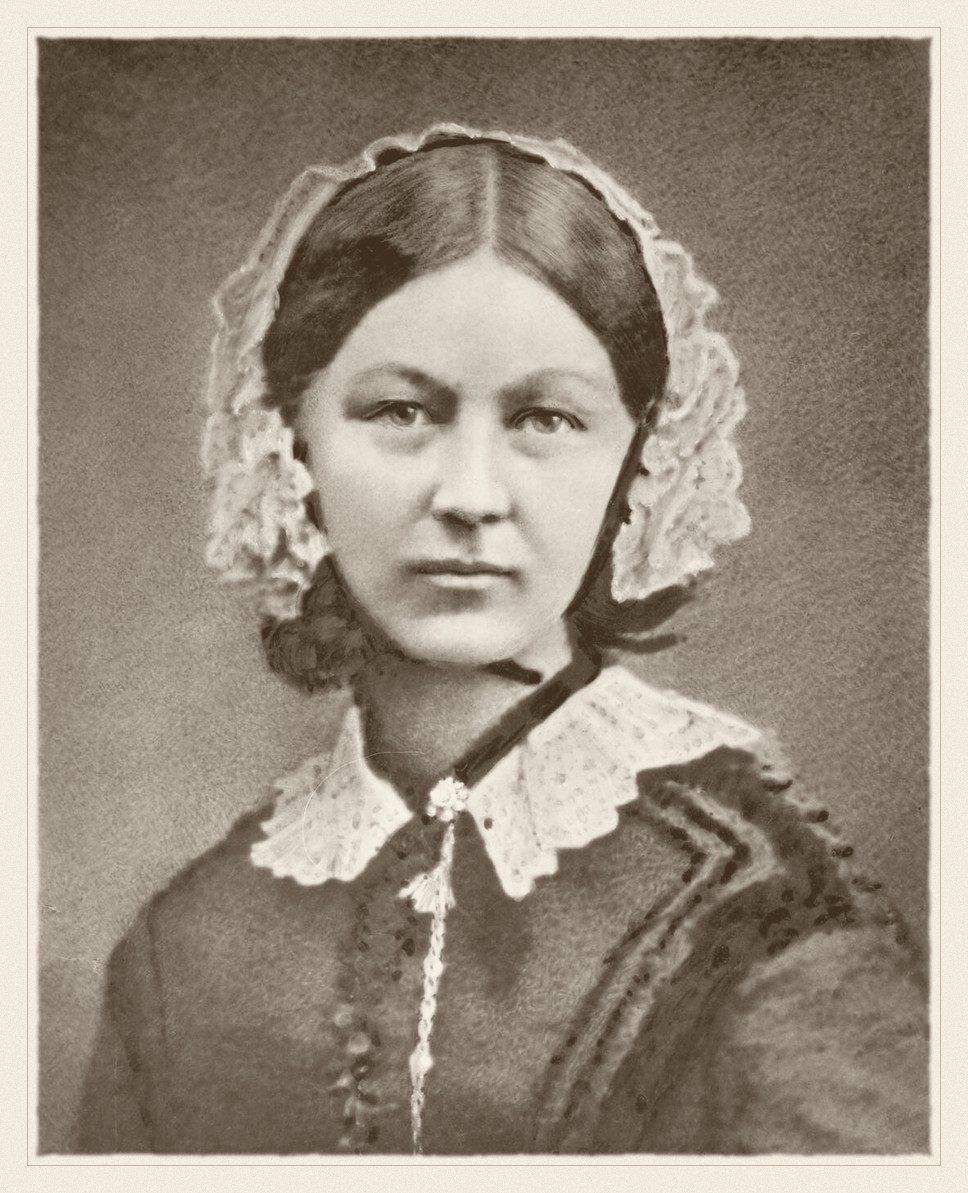
\includegraphics[keepaspectratio]{images/session-02-nightingale.jpg}}

\textbf{Florence Nightingale} · \textbf{1820--1910}

Made the case with a chart rather than a table, and changed policy with
it.

{Hering, circa 1857-1858. Public domain, via Wikimedia Commons.}

\end{qmibplate}

\begin{qmibarchive}

\textbf{From the archive · Nightingale, 1858}

Florence Nightingale returned from the Crimea with an argument and a
table. The argument was that most of the army's dead had been killed by
preventable disease rather than by the enemy, and that sanitary reform
would therefore save more soldiers than anything the surgeons could do.
The table was ignored.

So she drew it. Her polar-area diagram --- the ``coxcomb'' --- put each
month around a circle and the deaths in each as an area, split by cause,
and the blue wedge of preventable disease overwhelmed everything else on
sight. The chart was circulated to a royal commission, to ministers, to
the Queen. The reforms followed.

The lesson is not that charts are prettier than tables. It is that a
table asks the reader to hold twenty-four numbers in their head and
perform the comparison themselves, while a chart performs the comparison
for them. Human visual judgement is very good at some comparisons ---
position along a common scale, most of all --- and poor at others, and
that ordering has since been measured rather than assumed
(\citeproc{ref-cleveland1984}{Cleveland and McGill 1984}). Nightingale
had no such research. She had the intuition, and a commission that
needed convincing.

\begin{Shaded}
\begin{Highlighting}[]
\ImportTok{import}\NormalTok{ sys, warnings}
\NormalTok{sys.path.insert(}\DecValTok{0}\NormalTok{, }\StringTok{"../slides"}\NormalTok{)}\OperatorTok{;}\NormalTok{ sys.path.insert(}\DecValTok{0}\NormalTok{, }\StringTok{".."}\NormalTok{)}
\NormalTok{warnings.filterwarnings(}\StringTok{"ignore"}\NormalTok{)}
\ImportTok{from}\NormalTok{ plotstyle }\ImportTok{import}\NormalTok{ setup, CL}
\NormalTok{plt }\OperatorTok{=}\NormalTok{ setup()}

\ImportTok{import}\NormalTok{ numpy }\ImportTok{as}\NormalTok{ np, pandas }\ImportTok{as}\NormalTok{ pd, qmib}

\NormalTok{core }\OperatorTok{=}\NormalTok{ qmib.load(}\StringTok{"core"}\NormalTok{)}
\NormalTok{by\_year }\OperatorTok{=}\NormalTok{ core.groupby(}\StringTok{"time"}\NormalTok{)[}\StringTok{"gdp\_pc\_eur"}\NormalTok{].mean().dropna()}

\NormalTok{fig, (ax\_t, ax\_c) }\OperatorTok{=}\NormalTok{ plt.subplots(}\DecValTok{1}\NormalTok{, }\DecValTok{2}\NormalTok{, figsize}\OperatorTok{=}\NormalTok{(}\FloatTok{9.4}\NormalTok{, }\FloatTok{4.2}\NormalTok{),}
\NormalTok{                                 gridspec\_kw}\OperatorTok{=}\NormalTok{\{}\StringTok{"width\_ratios"}\NormalTok{: [}\DecValTok{1}\NormalTok{, }\FloatTok{1.5}\NormalTok{]\})}

\NormalTok{ax\_t.axis(}\StringTok{"off"}\NormalTok{)}
\NormalTok{rows }\OperatorTok{=}\NormalTok{ [}\SpecialStringTok{f"}\SpecialCharTok{\{}\BuiltInTok{int}\NormalTok{(y)}\SpecialCharTok{\}}\SpecialStringTok{    }\SpecialCharTok{\{}\NormalTok{v}\SpecialCharTok{:\textgreater{}10,.0f\}}\SpecialStringTok{"} \ControlFlowTok{for}\NormalTok{ y, v }\KeywordTok{in}\NormalTok{ by\_year.items()]}
\NormalTok{ax\_t.text(}\FloatTok{0.5}\NormalTok{, }\FloatTok{0.5}\NormalTok{, }\StringTok{"year        mean}\CharTok{\textbackslash{}n}\StringTok{"} \OperatorTok{+} \StringTok{"}\CharTok{\textbackslash{}n}\StringTok{"}\NormalTok{.join(rows),}
\NormalTok{          family}\OperatorTok{=}\StringTok{"monospace"}\NormalTok{, fontsize}\OperatorTok{=}\FloatTok{8.5}\NormalTok{, va}\OperatorTok{=}\StringTok{"center"}\NormalTok{, ha}\OperatorTok{=}\StringTok{"center"}\NormalTok{,}
\NormalTok{          transform}\OperatorTok{=}\NormalTok{ax\_t.transAxes, color}\OperatorTok{=}\NormalTok{CL.ink)}
\NormalTok{ax\_t.set\_title(}\StringTok{"as a table"}\NormalTok{, fontsize}\OperatorTok{=}\DecValTok{10}\NormalTok{, loc}\OperatorTok{=}\StringTok{"left"}\NormalTok{)}

\NormalTok{ax\_c.plot(by\_year.index, by\_year.values, marker}\OperatorTok{=}\StringTok{"o"}\NormalTok{, ms}\OperatorTok{=}\FloatTok{4.5}\NormalTok{, lw}\OperatorTok{=}\FloatTok{1.8}\NormalTok{, color}\OperatorTok{=}\NormalTok{CL.accent)}
\NormalTok{ax\_c.set\_ylabel(}\StringTok{"mean GDP per capita (EUR)"}\NormalTok{)}
\NormalTok{ax\_c.set\_title(}\StringTok{"as position along a common scale"}\NormalTok{, fontsize}\OperatorTok{=}\DecValTok{10}\NormalTok{, loc}\OperatorTok{=}\StringTok{"left"}\NormalTok{)}
\NormalTok{ax\_c.margins(x}\OperatorTok{=}\FloatTok{0.04}\NormalTok{)}

\NormalTok{fig.tight\_layout()}
\end{Highlighting}
\end{Shaded}

\begin{figure}[htbp]

\centering{

\pandocbounded{
\includegraphics[keepaspectratio]{session-02_files/figure-pdf/fig-table-vs-chart-output-1.png}}

}

\caption{\label{fig-table-vs-chart}The same fourteen numbers, twice.
Average GDP per capita by year in the course fixtures, as a table of
figures and as position along a common scale. Nothing has been added on
the right; the comparison has simply been done for you.}

\end{figure}%

\end{qmibarchive}

\section{Look at it first, literally}\label{look-at-it-first-literally}

Before any statistic, look at the thing. R users have \texttt{View()};
Python has no single equivalent, because a notebook renders the last
expression, a script prints nothing, and \texttt{print(df)} truncates to
the terminal width. \texttt{qmib.view()} gives the same answer in all
three: the shape, every column with its type and how much of it is
missing, and the first rows --- scrollable here, printed in a terminal.

\phantomsection\label{view-core}
\begin{Shaded}
\begin{Highlighting}[]
\NormalTok{qmib.view(core)}
\end{Highlighting}
\end{Shaded}

\begin{verbatim}
core: 450 rows x 11 columns  (2.7% missing overall)
\end{verbatim}

\phantomsection\label{view-core-1}
\begin{landscape}\thispagestyle{empty}\begingroup\scriptsize

\begin{longtable}[]{@{}llllllllllll@{}}
\caption{}\label{T_5a9cb}\tabularnewline
\toprule\noalign{}
~ & geo & time & gdp\_pc\_eur & population & employment\_ths &
productivity\_idx & gfcf\_meur & prod\_growth & falling\_behind &
falling\_behind\_next & flag \\
\midrule\noalign{}
\endfirsthead
\toprule\noalign{}
~ & geo & time & gdp\_pc\_eur & population & employment\_ths &
productivity\_idx & gfcf\_meur & prod\_growth & falling\_behind &
falling\_behind\_next & flag \\
\midrule\noalign{}
\endhead
\bottomrule\noalign{}
\endlastfoot
0 & AT & 2010 & 38193.955 & 11495826.000 & 5265.073 & 103.349 & 95.222 &
--- & 0 & 0 & \\
1 & AT & 2011 & 40644.251 & 12299989.000 & 5830.411 & 106.119 & 108.808
& 2.681 & 0 & 0 & \\
2 & AT & 2012 & 33035.780 & 12294814.000 & 5746.553 & 108.084 & 87.626 &
--- & 0 & 0 & \\
3 & AT & 2013 & 33595.312 & 11768544.000 & 5146.733 & 104.292 & 85.048 &
-3.508 & 0 & 0 & \\
4 & AT & 2014 & 37265.749 & 11949079.000 & 5218.544 & 104.665 & 94.471 &
0.358 & 0 & 0 & \\
5 & AT & 2015 & 23723.422 & 11555339.000 & 5094.443 & 105.127 & 57.017 &
0.441 & 0 & 1 & \\
6 & AT & 2016 & 29535.812 & 13053057.000 & 5878.256 & 100.782 & 80.190 &
-4.133 & 1 & 0 & \\
7 & AT & 2017 & --- & 11379421.000 & 5042.292 & 108.135 & 56.972 & 7.296
& 0 & 1 & \\
8 & AT & 2018 & 29754.420 & 12290876.000 & 5566.416 & --- & 76.404 &
-3.278 & 1 & 0 & \\
9 & AT & 2019 & 32816.404 & 12562395.000 & 5648.978 & 108.299 & 86.547 &
3.546 & 0 & 0 & \\
10 & AT & 2020 & 28031.533 & 10963179.000 & 4655.423 & 104.708 & 64.633
& -3.316 & 0 & 0 & \\
11 & AT & 2021 & 22314.188 & 11769447.000 & 5044.122 & 106.423 & 54.926
& 1.638 & 0 & 0 & \\
\end{longtable}

\endgroup\end{landscape}

\phantomsection\label{view-core-2}
\begin{longtable}[]{@{}llll@{}}
\toprule\noalign{}
& dtype & missing & distinct \\
\midrule\noalign{}
\endhead
\bottomrule\noalign{}
\endlastfoot
geo & str & 0.0\% & 30 \\
time & int64 & 0.0\% & 15 \\
gdp\_pc\_eur & float64 & 2.9\% & 437 \\
population & float64 & 3.3\% & 435 \\
employment\_ths & float64 & 1.3\% & 444 \\
productivity\_idx & float64 & 2.4\% & 434 \\
gfcf\_meur & float64 & 4.0\% & 432 \\
prod\_growth & float64 & 9.3\% & 399 \\
falling\_behind & Int64 & 0.0\% & 2 \\
falling\_behind\_next & Int64 & 6.7\% & 2 \\
flag & str & 0.0\% & 5 \\
\end{longtable}

Two things in that table are worth noticing before going further, and
both are invisible in any summary statistic. Seven of the eleven columns
have missing values, and \texttt{prod\_growth} is missing far more often
than the rest --- a pattern this chapter returns to. And \texttt{flag}
has five distinct values in a column that looks like it should be empty,
which is the observation-status code the source uses to mark provisional
and estimated figures.

\section{Centre: three answers, three
questions}\label{centre-three-answers-three-questions}

The first question about a variable is where it sits. There are three
standard answers and they are not interchangeable --- each is the
solution to a different problem.

\begin{qmibdefinition}

{\textbf{Mean}} --- \(\bar x = \frac1n \sum_i x_i\). The value
minimising the sum of \emph{squared} deviations, and the balance point
of the distribution. It uses every observation, which is its strength
and its weakness: one extreme value moves it without limit.

\end{qmibdefinition}

\begin{qmibdefinition}

{\textbf{Median}} --- the middle order statistic, minimising the sum of
\emph{absolute} deviations. It ignores how far away the extremes are,
only that they are on one side, so it is unmoved by an outlier of any
magnitude. Its breakdown point is 50\%: half the data must be corrupted
before it fails.

\end{qmibdefinition}

\begin{qmibdefinition}

{\textbf{Trimmed mean}} --- the mean of the data after discarding the
most extreme \(\alpha\) from each tail. A deliberate compromise: more
efficient than the median when the distribution is nearly normal, more
robust than the mean when it is not.

\end{qmibdefinition}

Which to report is a question about the decision the number will serve.
If you are budgeting a total --- total tax revenue, total emissions ---
the mean is the right summary, because the total \emph{is} the mean
times the count and the extremes genuinely contribute. If you are
describing a typical case --- what a typical country looks like --- the
median is right, because the question is about the middle and not about
the total.

\phantomsection\label{check-centre}
\begin{Shaded}
\begin{Highlighting}[]
\ImportTok{from}\NormalTok{ scipy }\ImportTok{import}\NormalTok{ stats}

\NormalTok{y }\OperatorTok{=}\NormalTok{ core[}\StringTok{"gdp\_pc\_eur"}\NormalTok{].dropna()}
\NormalTok{mean, median }\OperatorTok{=}\NormalTok{ y.mean(), y.median()}
\NormalTok{trimmed }\OperatorTok{=}\NormalTok{ stats.trim\_mean(y, }\FloatTok{0.10}\NormalTok{)}

\BuiltInTok{print}\NormalTok{(}\SpecialStringTok{f"n = }\SpecialCharTok{\{}\BuiltInTok{len}\NormalTok{(y)}\SpecialCharTok{\}}\SpecialStringTok{   (of }\SpecialCharTok{\{}\BuiltInTok{len}\NormalTok{(core)}\SpecialCharTok{\}}\SpecialStringTok{ rows; }\SpecialCharTok{\{}\NormalTok{core[}\StringTok{\textquotesingle{}gdp\_pc\_eur\textquotesingle{}}\NormalTok{]}\SpecialCharTok{.}\NormalTok{isna()}\SpecialCharTok{.}\BuiltInTok{sum}\NormalTok{()}\SpecialCharTok{\}}\SpecialStringTok{ missing)"}\NormalTok{)}
\BuiltInTok{print}\NormalTok{(}\SpecialStringTok{f"  mean          }\SpecialCharTok{\{}\NormalTok{mean}\SpecialCharTok{:\textgreater{}10,.0f\}}\SpecialStringTok{"}\NormalTok{)}
\BuiltInTok{print}\NormalTok{(}\SpecialStringTok{f"  10\% trimmed   }\SpecialCharTok{\{}\NormalTok{trimmed}\SpecialCharTok{:\textgreater{}10,.0f\}}\SpecialStringTok{"}\NormalTok{)}
\BuiltInTok{print}\NormalTok{(}\SpecialStringTok{f"  median        }\SpecialCharTok{\{}\NormalTok{median}\SpecialCharTok{:\textgreater{}10,.0f\}}\SpecialStringTok{"}\NormalTok{)}
\BuiltInTok{print}\NormalTok{(}\SpecialStringTok{f"}\CharTok{\textbackslash{}n}\SpecialStringTok{mean {-} median = }\SpecialCharTok{\{}\NormalTok{mean }\OperatorTok{{-}}\NormalTok{ median}\SpecialCharTok{:,.0f\}}\SpecialStringTok{, which is }\SpecialCharTok{\{}\NormalTok{(mean}\OperatorTok{/}\NormalTok{median }\OperatorTok{{-}} \DecValTok{1}\NormalTok{)}\SpecialCharTok{:.1\%\}}\SpecialStringTok{ of the median."}\NormalTok{)}
\BuiltInTok{print}\NormalTok{(}\StringTok{"A mean above the median is the signature of a right tail."}\NormalTok{)}
\end{Highlighting}
\end{Shaded}

\begin{verbatim}
n = 437   (of 450 rows; 13 missing)
  mean              30,373
  10% trimmed       28,723
  median            25,733

mean - median = 4,639, which is 18.0% of the median.
A mean above the median is the signature of a right tail.
\end{verbatim}

The mean sits well above the median here, and the trimmed mean sits
between them --- the ordering that a right-skewed variable always
produces. Reporting the mean alone would describe a country that does
not exist: richer than most of the sample, because a few very rich
country-years are pulling it up.

\section{\texorpdfstring{Spread, and the \(n-1\) that everyone asks
about}{Spread, and the n-1 that everyone asks about}}\label{spread-and-the-n-1-that-everyone-asks-about}

\begin{qmibdefinition}

{\textbf{Sample variance}} --- \[
s^2 \;=\; \frac{1}{n-1}\sum_i (x_i - \bar x)^2 .
\] The divisor is \(n-1\), not \(n\), because the deviations are taken
from \(\bar x\) rather than from the true mean \(\mu\). \(\bar x\) is
the value that \emph{minimises} that sum of squares, so deviations from
it are systematically too small, and dividing by \(n\) would return an
estimate that is too low on average. One degree of freedom was spent
estimating the centre; \(n-1\) remain.

\end{qmibdefinition}

That is the honest one-sentence answer, and it is worth being able to
demonstrate rather than assert. The cell below does it by simulation:
draw many samples from a distribution whose variance is known, and
compare the average of the two estimators against the truth.

\phantomsection\label{check-n-minus-1}
\begin{Shaded}
\begin{Highlighting}[]
\NormalTok{rng }\OperatorTok{=}\NormalTok{ np.random.default\_rng(}\DecValTok{60033}\NormalTok{)}
\NormalTok{true\_var, n, reps }\OperatorTok{=} \FloatTok{4.0}\NormalTok{, }\DecValTok{5}\NormalTok{, }\DecValTok{200\_000}
\NormalTok{draws }\OperatorTok{=}\NormalTok{ rng.normal(}\DecValTok{0}\NormalTok{, np.sqrt(true\_var), size}\OperatorTok{=}\NormalTok{(reps, n))}
\NormalTok{dev2 }\OperatorTok{=}\NormalTok{ ((draws }\OperatorTok{{-}}\NormalTok{ draws.mean(axis}\OperatorTok{=}\DecValTok{1}\NormalTok{, keepdims}\OperatorTok{=}\VariableTok{True}\NormalTok{)) }\OperatorTok{**} \DecValTok{2}\NormalTok{).}\BuiltInTok{sum}\NormalTok{(axis}\OperatorTok{=}\DecValTok{1}\NormalTok{)}

\BuiltInTok{print}\NormalTok{(}\SpecialStringTok{f"true variance                 }\SpecialCharTok{\{}\NormalTok{true\_var}\SpecialCharTok{:.4f\}}\SpecialStringTok{"}\NormalTok{)}
\BuiltInTok{print}\NormalTok{(}\SpecialStringTok{f"average of  sum/(n)    (biased)   }\SpecialCharTok{\{}\NormalTok{(dev2 }\OperatorTok{/}\NormalTok{ n)}\SpecialCharTok{.}\NormalTok{mean()}\SpecialCharTok{:.4f\}}\SpecialStringTok{"}\NormalTok{)}
\BuiltInTok{print}\NormalTok{(}\SpecialStringTok{f"average of  sum/(n{-}1)  (unbiased) }\SpecialCharTok{\{}\NormalTok{(dev2 }\OperatorTok{/}\NormalTok{ (n }\OperatorTok{{-}} \DecValTok{1}\NormalTok{))}\SpecialCharTok{.}\NormalTok{mean()}\SpecialCharTok{:.4f\}}\SpecialStringTok{"}\NormalTok{)}
\BuiltInTok{print}\NormalTok{(}\SpecialStringTok{f"}\CharTok{\textbackslash{}n}\SpecialStringTok{the biased estimator is low by a factor of about }\SpecialCharTok{\{}\NormalTok{(n}\OperatorTok{{-}}\DecValTok{1}\NormalTok{)}\OperatorTok{/}\NormalTok{n}\SpecialCharTok{:.2f\}}\SpecialStringTok{ = (n{-}1)/n"}\NormalTok{)}
\end{Highlighting}
\end{Shaded}

\begin{verbatim}
true variance                 4.0000
average of  sum/(n)    (biased)   3.2017
average of  sum/(n-1)  (unbiased) 4.0021

the biased estimator is low by a factor of about 0.80 = (n-1)/n
\end{verbatim}

With \(n = 5\) the understatement is 20\%, which is not a rounding
error. It shrinks as \(n\) grows, which is why the choice rarely matters
in a large sample and matters a great deal in a small one.

The variance is in squared units --- squared euros, here, which is not a
quantity anyone has an intuition for --- so it is normally reported as
its square root, the standard deviation. The alternative measure of
spread makes no distributional assumption at all:

\begin{qmibdefinition}

{\textbf{Interquartile range}} --- \(\mathrm{IQR} = Q_3 - Q_1\), the
width of the middle half of the data. Like the median it is unaffected
by the size of the extremes, and like the median it is the right choice
when the distribution is skewed or heavy-tailed.

\end{qmibdefinition}

\section{Shape, and a rule that passes when it should
not}\label{shape-and-a-rule-that-passes-when-it-should-not}

Two standardised moments describe departure from the normal shape.

\begin{qmibdefinition}

{\textbf{Skewness}} --- the third standardised moment,
\(g_1 = \frac1n \sum_i \left(\frac{x_i - \bar x}{s}\right)^3\). Zero for
any symmetric distribution; positive when the right tail is longer. The
cube preserves sign, so observations far above the mean contribute
positively and those far below negatively, and they do not cancel unless
the distribution is symmetric.

\end{qmibdefinition}

\begin{qmibdefinition}

{\textbf{Excess kurtosis}} --- the fourth standardised moment minus 3,
so that a normal distribution scores zero. Positive means heavier tails
than normal --- more extreme observations than a normal would produce.
It is \emph{not} a measure of ``peakedness'', a description that
survives in textbooks and is wrong.

\end{qmibdefinition}

The conventional threshold is that \(|g_1| > 2\) or \(|g_2| > 2\)
indicates a serious departure. Now watch what happens when the same
variable is tested by the empirical rule instead.

\phantomsection\label{check-shape}
\begin{Shaded}
\begin{Highlighting}[]
\NormalTok{skew }\OperatorTok{=}\NormalTok{ stats.skew(y, bias}\OperatorTok{=}\VariableTok{False}\NormalTok{)}
\NormalTok{kurt }\OperatorTok{=}\NormalTok{ stats.kurtosis(y, bias}\OperatorTok{=}\VariableTok{False}\NormalTok{)          }\CommentTok{\# already excess}
\NormalTok{sd }\OperatorTok{=}\NormalTok{ y.std(ddof}\OperatorTok{=}\DecValTok{1}\NormalTok{)}

\BuiltInTok{print}\NormalTok{(}\SpecialStringTok{f"skewness          }\SpecialCharTok{\{}\NormalTok{skew}\SpecialCharTok{:+.3f\}}\SpecialStringTok{   (threshold ±2)"}\NormalTok{)}
\BuiltInTok{print}\NormalTok{(}\SpecialStringTok{f"excess kurtosis   }\SpecialCharTok{\{}\NormalTok{kurt}\SpecialCharTok{:+.3f\}}\SpecialStringTok{   (threshold ±2)"}\NormalTok{)}
\BuiltInTok{print}\NormalTok{(}\SpecialStringTok{f"}\CharTok{\textbackslash{}n}\SpecialStringTok{empirical rule — the fraction of observations within k standard deviations:"}\NormalTok{)}
\ControlFlowTok{for}\NormalTok{ k, expected }\KeywordTok{in}\NormalTok{ ((}\DecValTok{1}\NormalTok{, }\FloatTok{0.68}\NormalTok{), (}\DecValTok{2}\NormalTok{, }\FloatTok{0.95}\NormalTok{), (}\DecValTok{3}\NormalTok{, }\FloatTok{0.997}\NormalTok{)):}
\NormalTok{    got }\OperatorTok{=}\NormalTok{ ((y }\OperatorTok{{-}}\NormalTok{ y.mean()).}\BuiltInTok{abs}\NormalTok{() }\OperatorTok{\textless{}}\NormalTok{ k }\OperatorTok{*}\NormalTok{ sd).mean()}
    \BuiltInTok{print}\NormalTok{(}\SpecialStringTok{f"  within }\SpecialCharTok{\{}\NormalTok{k}\SpecialCharTok{\}}\SpecialStringTok{ sd   }\SpecialCharTok{\{}\NormalTok{got}\SpecialCharTok{:6.1\%\}}\SpecialStringTok{   normal says }\SpecialCharTok{\{}\NormalTok{expected}\SpecialCharTok{:.1\%\}}\SpecialStringTok{"}\NormalTok{)}
\end{Highlighting}
\end{Shaded}

\begin{verbatim}
skewness          +0.887   (threshold ±2)
excess kurtosis   +0.014   (threshold ±2)

empirical rule — the fraction of observations within k standard deviations:
  within 1 sd    68.0%   normal says 68.0%
  within 2 sd    95.7%   normal says 95.0%
  within 3 sd    99.3%   normal says 99.7%
\end{verbatim}

Read that carefully, because it is the point of the section. The
variable is visibly right-skewed --- the mean exceeds the median by a
wide margin, and the skewness statistic agrees. Yet the empirical rule
is satisfied almost exactly: 68\% within one standard deviation, close
to 95\% within two.

The empirical rule is a \emph{weak} check. It constrains the bulk of the
distribution, where skew has little effect, and says almost nothing
about the tails, which is where the departure lives. Passing it is not
evidence of normality. Its precondition is the thing being tested, which
makes it useless as a test and merely reassuring as a description --- a
distinction worth carrying into every diagnostic in this book.

\section{Transformation, and what it
costs}\label{transformation-and-what-it-costs}

The standard response to a right-skewed positive variable is to take
logarithms. It works, in the sense that the skew largely disappears. It
is worth watching what else changes.

\begin{Shaded}
\begin{Highlighting}[]
\NormalTok{ly }\OperatorTok{=}\NormalTok{ np.log(y)}
\NormalTok{fig, axes }\OperatorTok{=}\NormalTok{ plt.subplots(}\DecValTok{1}\NormalTok{, }\DecValTok{2}\NormalTok{, figsize}\OperatorTok{=}\NormalTok{(}\FloatTok{9.4}\NormalTok{, }\FloatTok{3.8}\NormalTok{))}

\ControlFlowTok{for}\NormalTok{ ax, series, name }\KeywordTok{in}\NormalTok{ ((axes[}\DecValTok{0}\NormalTok{], y, }\StringTok{"GDP per capita (EUR)"}\NormalTok{),}
\NormalTok{                         (axes[}\DecValTok{1}\NormalTok{], ly, }\StringTok{"log GDP per capita"}\NormalTok{)):}
\NormalTok{    ax.hist(series, bins}\OperatorTok{=}\DecValTok{32}\NormalTok{, color}\OperatorTok{=}\NormalTok{CL.accent, alpha}\OperatorTok{=}\FloatTok{0.55}\NormalTok{, edgecolor}\OperatorTok{=}\StringTok{"white"}\NormalTok{, linewidth}\OperatorTok{=}\FloatTok{0.6}\NormalTok{)}
\NormalTok{    ax.axvline(series.mean(), color}\OperatorTok{=}\NormalTok{CL.warn, lw}\OperatorTok{=}\FloatTok{1.8}\NormalTok{, label}\OperatorTok{=}\StringTok{"mean"}\NormalTok{)}
\NormalTok{    ax.axvline(series.median(), color}\OperatorTok{=}\NormalTok{CL.warn, lw}\OperatorTok{=}\FloatTok{1.5}\NormalTok{, ls}\OperatorTok{=}\StringTok{"{-}{-}"}\NormalTok{, label}\OperatorTok{=}\StringTok{"median"}\NormalTok{)}
\NormalTok{    ax.set\_xlabel(name)}
\NormalTok{    ax.set\_title(}\SpecialStringTok{f"skew }\SpecialCharTok{\{}\NormalTok{stats}\SpecialCharTok{.}\NormalTok{skew(series, bias}\OperatorTok{=}\VariableTok{False}\NormalTok{)}\SpecialCharTok{:+.2f\}}\SpecialStringTok{   "}
                 \SpecialStringTok{f"excess kurtosis }\SpecialCharTok{\{}\NormalTok{stats}\SpecialCharTok{.}\NormalTok{kurtosis(series, bias}\OperatorTok{=}\VariableTok{False}\NormalTok{)}\SpecialCharTok{:+.2f\}}\SpecialStringTok{"}\NormalTok{,}
\NormalTok{                 fontsize}\OperatorTok{=}\FloatTok{9.5}\NormalTok{, loc}\OperatorTok{=}\StringTok{"left"}\NormalTok{)}
\NormalTok{axes[}\DecValTok{0}\NormalTok{].set\_ylabel(}\StringTok{"count"}\NormalTok{)}
\NormalTok{axes[}\DecValTok{0}\NormalTok{].legend(frameon}\OperatorTok{=}\VariableTok{False}\NormalTok{, fontsize}\OperatorTok{=}\FloatTok{8.5}\NormalTok{)}
\NormalTok{fig.tight\_layout()}
\end{Highlighting}
\end{Shaded}

\begin{figure}[htbp]

\centering{

\pandocbounded{
\includegraphics[keepaspectratio]{session-02_files/figure-pdf/fig-distribution-output-1.png}}

}

\caption{\label{fig-distribution}GDP per capita in the course fixtures,
raw and log-transformed, with mean (solid) and median (dashed). Taking
logs removes most of the skew; look at what it does to the tails.}

\end{figure}%

The skew falls almost to zero, as advertised. The excess kurtosis moves
the other way, from very slightly positive to clearly negative --- the
transformed variable has \emph{lighter} tails than a normal
distribution, not merely lighter than before. Taking logs did not make
the variable normal. It made it a different non-normal shape.

That is the general situation, and it is why ``take logs to fix
normality'' is bad advice stated that way. The good reasons to take logs
are substantive: because the effect you believe in is proportional
rather than additive, because the variable is a ratio or a price, or
because the relationship you are about to model is multiplicative. If
those hold, the transformation is right whatever it does to the shape
statistics. If they do not, you have changed the quantity you are
modelling in order to improve a diagnostic, which is the tail wagging
the dog.

\section{What is missing, and why}\label{what-is-missing-and-why}

A summary of the observed values says nothing about the values that are
absent, and absence is rarely accidental.

\begin{qmibdefinition}

{\textbf{MCAR, MAR, MNAR}} --- Rubin's taxonomy
(\citeproc{ref-rubin1976}{DONALD B. Rubin 1976}). \emph{Missing
completely at random}: the probability of being missing is unrelated to
anything, observed or not --- the only case where dropping incomplete
rows is harmless. \emph{Missing at random}: the probability depends on
observed variables, so it can be modelled. \emph{Missing not at random}:
it depends on the unobserved value itself --- the highest incomes are
the ones not reported --- which cannot be diagnosed from the data alone,
because the evidence you would need is precisely what is missing.

\end{qmibdefinition}

\begin{Shaded}
\begin{Highlighting}[]
\NormalTok{cols }\OperatorTok{=}\NormalTok{ [}\StringTok{"gdp\_pc\_eur"}\NormalTok{, }\StringTok{"population"}\NormalTok{, }\StringTok{"employment\_ths"}\NormalTok{,}
        \StringTok{"productivity\_idx"}\NormalTok{, }\StringTok{"gfcf\_meur"}\NormalTok{, }\StringTok{"prod\_growth"}\NormalTok{]}
\NormalTok{grid }\OperatorTok{=}\NormalTok{ (core.pivot\_table(index}\OperatorTok{=}\StringTok{"geo"}\NormalTok{, columns}\OperatorTok{=}\StringTok{"time"}\NormalTok{, values}\OperatorTok{=}\NormalTok{cols,}
\NormalTok{                         aggfunc}\OperatorTok{=}\StringTok{"first"}\NormalTok{, dropna}\OperatorTok{=}\VariableTok{False}\NormalTok{)}
\NormalTok{        .isna())}

\NormalTok{fig, ax }\OperatorTok{=}\NormalTok{ plt.subplots(figsize}\OperatorTok{=}\NormalTok{(}\FloatTok{9.2}\NormalTok{, }\FloatTok{3.4}\NormalTok{))}
\NormalTok{share }\OperatorTok{=}\NormalTok{ pd.DataFrame(\{c: grid[c].mean(axis}\OperatorTok{=}\DecValTok{0}\NormalTok{) }\ControlFlowTok{for}\NormalTok{ c }\KeywordTok{in}\NormalTok{ cols\}).T}
\NormalTok{im }\OperatorTok{=}\NormalTok{ ax.imshow(share.values, aspect}\OperatorTok{=}\StringTok{"auto"}\NormalTok{, cmap}\OperatorTok{=}\StringTok{"bone\_r"}\NormalTok{, vmin}\OperatorTok{=}\DecValTok{0}\NormalTok{, vmax}\OperatorTok{=}\DecValTok{1}\NormalTok{)}
\NormalTok{ax.set\_yticks(}\BuiltInTok{range}\NormalTok{(}\BuiltInTok{len}\NormalTok{(cols)))}\OperatorTok{;}\NormalTok{ ax.set\_yticklabels(cols, fontsize}\OperatorTok{=}\FloatTok{8.5}\NormalTok{)}
\NormalTok{ax.set\_xticks(}\BuiltInTok{range}\NormalTok{(}\BuiltInTok{len}\NormalTok{(share.columns)))}
\NormalTok{ax.set\_xticklabels([}\BuiltInTok{int}\NormalTok{(t) }\ControlFlowTok{for}\NormalTok{ t }\KeywordTok{in}\NormalTok{ share.columns], fontsize}\OperatorTok{=}\DecValTok{8}\NormalTok{, rotation}\OperatorTok{=}\DecValTok{90}\NormalTok{)}
\NormalTok{ax.set\_title(}\StringTok{"share of countries missing, by variable and year"}\NormalTok{, fontsize}\OperatorTok{=}\DecValTok{10}\NormalTok{, loc}\OperatorTok{=}\StringTok{"left"}\NormalTok{)}
\NormalTok{fig.colorbar(im, ax}\OperatorTok{=}\NormalTok{ax, fraction}\OperatorTok{=}\FloatTok{0.025}\NormalTok{, pad}\OperatorTok{=}\FloatTok{0.01}\NormalTok{)}
\NormalTok{fig.tight\_layout()}
\end{Highlighting}
\end{Shaded}

\begin{figure}[htbp]

\centering{

\pandocbounded{
\includegraphics[keepaspectratio]{session-02_files/figure-pdf/fig-missing-output-1.png}}

}

\caption{\label{fig-missing}Missingness in the course fixtures. Each
cell is one country-year; dark means absent. The pattern is not noise
--- read the first column.}

\end{figure}%

\phantomsection\label{check-missing}
\begin{Shaded}
\begin{Highlighting}[]
\NormalTok{miss }\OperatorTok{=}\NormalTok{ core[}\StringTok{"prod\_growth"}\NormalTok{].isna()}
\BuiltInTok{print}\NormalTok{(}\SpecialStringTok{f"prod\_growth missing: }\SpecialCharTok{\{}\NormalTok{miss}\SpecialCharTok{.}\BuiltInTok{sum}\NormalTok{()}\SpecialCharTok{\}}\SpecialStringTok{ of }\SpecialCharTok{\{}\BuiltInTok{len}\NormalTok{(core)}\SpecialCharTok{\}}\SpecialStringTok{ (}\SpecialCharTok{\{}\NormalTok{miss}\SpecialCharTok{.}\NormalTok{mean()}\SpecialCharTok{:.1\%\}}\SpecialStringTok{)"}\NormalTok{)}
\BuiltInTok{print}\NormalTok{(}\SpecialStringTok{f"  in 2010 alone:     }\SpecialCharTok{\{}\NormalTok{miss[core.time }\OperatorTok{==} \DecValTok{2010}\NormalTok{]}\SpecialCharTok{.}\NormalTok{mean()}\SpecialCharTok{:.0\%\}}\SpecialStringTok{"}\NormalTok{)}

\NormalTok{obs }\OperatorTok{=}\NormalTok{ core.dropna(subset}\OperatorTok{=}\NormalTok{[}\StringTok{"gdp\_pc\_eur"}\NormalTok{])}
\NormalTok{present }\OperatorTok{=}\NormalTok{ obs.loc[}\OperatorTok{\textasciitilde{}}\NormalTok{obs[}\StringTok{"prod\_growth"}\NormalTok{].isna(), }\StringTok{"gdp\_pc\_eur"}\NormalTok{].mean()}
\NormalTok{absent }\OperatorTok{=}\NormalTok{ obs.loc[obs[}\StringTok{"prod\_growth"}\NormalTok{].isna(), }\StringTok{"gdp\_pc\_eur"}\NormalTok{].mean()}
\BuiltInTok{print}\NormalTok{(}\SpecialStringTok{f"}\CharTok{\textbackslash{}n}\SpecialStringTok{mean GDP per capita where prod\_growth is present: }\SpecialCharTok{\{}\NormalTok{present}\SpecialCharTok{:\textgreater{}9,.0f\}}\SpecialStringTok{"}\NormalTok{)}
\BuiltInTok{print}\NormalTok{(}\SpecialStringTok{f"                          where it is missing:   }\SpecialCharTok{\{}\NormalTok{absent}\SpecialCharTok{:\textgreater{}9,.0f\}}\SpecialStringTok{"}\NormalTok{)}
\BuiltInTok{print}\NormalTok{(}\SpecialStringTok{f"  difference: }\SpecialCharTok{\{}\NormalTok{absent }\OperatorTok{{-}}\NormalTok{ present}\SpecialCharTok{:+,.0f\}}\SpecialStringTok{  (}\SpecialCharTok{\{}\NormalTok{(absent}\OperatorTok{/}\NormalTok{present }\OperatorTok{{-}} \DecValTok{1}\NormalTok{)}\SpecialCharTok{:+.1\%\}}\SpecialStringTok{)"}\NormalTok{)}
\BuiltInTok{print}\NormalTok{(}\StringTok{"}\CharTok{\textbackslash{}n}\StringTok{Missingness that depends on an observed variable is MAR, not MCAR."}\NormalTok{)}
\end{Highlighting}
\end{Shaded}

\begin{verbatim}
prod_growth missing: 42 of 450 (9.3%)
  in 2010 alone:     100%

mean GDP per capita where prod_growth is present:    30,023
                          where it is missing:      34,044
  difference: +4,021  (+13.4%)

Missingness that depends on an observed variable is MAR, not MCAR.
\end{verbatim}

Two findings, of different kinds. The first is structural and completely
explicable: \texttt{prod\_growth} is missing for \emph{every} country in
2010 because it is a year-on-year growth rate and 2010 is the first year
in the panel. There is no 2009 to difference against. That is not
missing data in any interesting sense --- it is a variable that does not
exist for that year, and treating it as an imputation problem would be a
category error.

The second is not structural. Where \texttt{prod\_growth} is absent, the
average GDP per capita differs materially from where it is present.
Missingness is associated with an observed variable, which puts it in
Rubin's \emph{missing at random} category and rules out the convenient
assumption. Dropping incomplete rows --- which every regression in this
book does by default --- is therefore not neutral: it changes the
composition of the sample toward the country-years that report. Whether
that matters depends on the question, and the only wrong move is not to
check.

\section{The first model, as a right-angled
triangle}\label{the-first-model-as-a-right-angled-triangle}

Now fit something. The simplest model relates one variable to one other,

\[
y_i \;=\; \beta_0 + \beta_1 x_i + \varepsilon_i ,
\]

and the least-squares solution in this case has a closed form worth
memorising, because it says what a slope \emph{is}:

\[
\hat\beta_1 \;=\; \frac{\operatorname{Cov}(x, y)}{\operatorname{Var}(x)},
\qquad
\hat\beta_0 \;=\; \bar y - \hat\beta_1 \bar x .
\]

The slope is covariation divided by variation in the predictor: how much
\(x\) and \(y\) move together, per unit of \(x\) moving at all. The
intercept exists only to make the line pass through
\((\bar x, \bar y)\), which it always does.

The geometry is where the understanding is. Think of the \(n\)
observations as a single vector in \(n\)-dimensional space. Centre it
--- work with \(y - \bar y\) --- and fitting a line is projecting that
vector onto the direction of \(x - \bar x\). The fitted values are the
shadow; the residuals are what the shadow misses; and because a
projection is orthogonal, the residual is at right angles to the fitted
vector. A right angle means Pythagoras:

\[
\underbrace{\lVert y - \bar y\rVert^2}_{\text{TSS}}
\;=\;
\underbrace{\lVert \hat y - \bar y\rVert^2}_{\text{ESS}}
\;+\;
\underbrace{\lVert y - \hat y\rVert^2}_{\text{RSS}} .
\]

That is the analysis of variance, and it is not an algebraic coincidence
--- it is the hypotenuse. Two consequences follow immediately.
\(R^2 = \mathrm{ESS} /
\mathrm{TSS}\) is \(\cos^2\) of the angle between the observed and
fitted vectors. And in a simple regression the correlation \(r\) is
exactly that cosine, so \(R^2 = r^2\) --- a fact usually presented as a
curiosity and actually a definition.

\phantomsection\label{check-triangle}
\begin{Shaded}
\begin{Highlighting}[]
\ImportTok{import}\NormalTok{ statsmodels.api }\ImportTok{as}\NormalTok{ sm}

\NormalTok{c }\OperatorTok{=}\NormalTok{ core.dropna(subset}\OperatorTok{=}\NormalTok{[}\StringTok{"gdp\_pc\_eur"}\NormalTok{, }\StringTok{"productivity\_idx"}\NormalTok{])}
\NormalTok{x, yv }\OperatorTok{=}\NormalTok{ c[}\StringTok{"productivity\_idx"}\NormalTok{].to\_numpy(), c[}\StringTok{"gdp\_pc\_eur"}\NormalTok{].to\_numpy()}

\NormalTok{b1 }\OperatorTok{=}\NormalTok{ np.cov(x, yv, ddof}\OperatorTok{=}\DecValTok{1}\NormalTok{)[}\DecValTok{0}\NormalTok{, }\DecValTok{1}\NormalTok{] }\OperatorTok{/}\NormalTok{ np.var(x, ddof}\OperatorTok{=}\DecValTok{1}\NormalTok{)}
\NormalTok{b0 }\OperatorTok{=}\NormalTok{ yv.mean() }\OperatorTok{{-}}\NormalTok{ b1 }\OperatorTok{*}\NormalTok{ x.mean()}
\NormalTok{fit }\OperatorTok{=}\NormalTok{ sm.OLS(yv, sm.add\_constant(x)).fit()}
\BuiltInTok{print}\NormalTok{(}\SpecialStringTok{f"slope by hand }\SpecialCharTok{\{}\NormalTok{b1}\SpecialCharTok{:12,.3f\}}\SpecialStringTok{   statsmodels }\SpecialCharTok{\{}\NormalTok{fit}\SpecialCharTok{.}\NormalTok{params[}\DecValTok{1}\NormalTok{]}\SpecialCharTok{:12,.3f\}}\SpecialStringTok{"}\NormalTok{)}
\BuiltInTok{print}\NormalTok{(}\SpecialStringTok{f"intercept     }\SpecialCharTok{\{}\NormalTok{b0}\SpecialCharTok{:12,.1f\}}\SpecialStringTok{   statsmodels }\SpecialCharTok{\{}\NormalTok{fit}\SpecialCharTok{.}\NormalTok{params[}\DecValTok{0}\NormalTok{]}\SpecialCharTok{:12,.1f\}}\SpecialStringTok{"}\NormalTok{)}

\NormalTok{tss }\OperatorTok{=}\NormalTok{ ((yv }\OperatorTok{{-}}\NormalTok{ yv.mean()) }\OperatorTok{**} \DecValTok{2}\NormalTok{).}\BuiltInTok{sum}\NormalTok{()}
\NormalTok{ess }\OperatorTok{=}\NormalTok{ ((fit.fittedvalues }\OperatorTok{{-}}\NormalTok{ yv.mean()) }\OperatorTok{**} \DecValTok{2}\NormalTok{).}\BuiltInTok{sum}\NormalTok{()}
\NormalTok{rss }\OperatorTok{=}\NormalTok{ (fit.resid }\OperatorTok{**} \DecValTok{2}\NormalTok{).}\BuiltInTok{sum}\NormalTok{()}
\BuiltInTok{print}\NormalTok{(}\SpecialStringTok{f"}\CharTok{\textbackslash{}n}\SpecialStringTok{TSS }\SpecialCharTok{\{}\NormalTok{tss}\SpecialCharTok{:.6e\}}\SpecialStringTok{"}\NormalTok{)}
\BuiltInTok{print}\NormalTok{(}\SpecialStringTok{f"ESS }\SpecialCharTok{\{}\NormalTok{ess}\SpecialCharTok{:.6e\}}\SpecialStringTok{"}\NormalTok{)}
\BuiltInTok{print}\NormalTok{(}\SpecialStringTok{f"RSS }\SpecialCharTok{\{}\NormalTok{rss}\SpecialCharTok{:.6e\}}\SpecialStringTok{"}\NormalTok{)}
\BuiltInTok{print}\NormalTok{(}\SpecialStringTok{f"TSS {-} (ESS + RSS) = }\SpecialCharTok{\{}\NormalTok{tss }\OperatorTok{{-}}\NormalTok{ ess }\OperatorTok{{-}}\NormalTok{ rss}\SpecialCharTok{:.3e\}}\SpecialStringTok{   (zero, to floating point)"}\NormalTok{)}

\NormalTok{r }\OperatorTok{=}\NormalTok{ np.corrcoef(x, yv)[}\DecValTok{0}\NormalTok{, }\DecValTok{1}\NormalTok{]}
\BuiltInTok{print}\NormalTok{(}\SpecialStringTok{f"}\CharTok{\textbackslash{}n}\SpecialStringTok{r = }\SpecialCharTok{\{}\NormalTok{r}\SpecialCharTok{:.6f\}}\SpecialStringTok{;  r² = }\SpecialCharTok{\{}\NormalTok{r}\OperatorTok{**}\DecValTok{2}\SpecialCharTok{:.6f\}}\SpecialStringTok{;  R² = }\SpecialCharTok{\{}\NormalTok{fit}\SpecialCharTok{.}\NormalTok{rsquared}\SpecialCharTok{:.6f\}}\SpecialStringTok{"}\NormalTok{)}
\BuiltInTok{print}\NormalTok{(}\SpecialStringTok{f"angle between the centred observed and fitted vectors: "}
      \SpecialStringTok{f"}\SpecialCharTok{\{}\NormalTok{np}\SpecialCharTok{.}\NormalTok{degrees(np.arccos(r))}\SpecialCharTok{:.2f\}}\SpecialStringTok{°"}\NormalTok{)}
\end{Highlighting}
\end{Shaded}

\begin{verbatim}
slope by hand    1,111.257   statsmodels    1,111.257
intercept        -86,118.1   statsmodels    -86,118.1

TSS 1.004705e+11
ESS 6.302104e+10
RSS 3.744941e+10
TSS - (ESS + RSS) = 7.629e-06   (zero, to floating point)

r = 0.791997;  r² = 0.627259;  R² = 0.627259
angle between the centred observed and fitted vectors: 37.63°
\end{verbatim}

\begin{Shaded}
\begin{Highlighting}[]
\NormalTok{fig, (axs, axg) }\OperatorTok{=}\NormalTok{ plt.subplots(}\DecValTok{1}\NormalTok{, }\DecValTok{2}\NormalTok{, figsize}\OperatorTok{=}\NormalTok{(}\FloatTok{9.4}\NormalTok{, }\FloatTok{4.2}\NormalTok{))}

\NormalTok{axs.scatter(x, yv, s}\OperatorTok{=}\DecValTok{14}\NormalTok{, color}\OperatorTok{=}\NormalTok{CL.accent, alpha}\OperatorTok{=}\FloatTok{0.45}\NormalTok{, edgecolor}\OperatorTok{=}\StringTok{"none"}\NormalTok{)}
\NormalTok{gx }\OperatorTok{=}\NormalTok{ np.linspace(x.}\BuiltInTok{min}\NormalTok{(), x.}\BuiltInTok{max}\NormalTok{(), }\DecValTok{50}\NormalTok{)}
\NormalTok{axs.plot(gx, b0 }\OperatorTok{+}\NormalTok{ b1 }\OperatorTok{*}\NormalTok{ gx, color}\OperatorTok{=}\NormalTok{CL.warn, lw}\OperatorTok{=}\DecValTok{2}\NormalTok{)}
\NormalTok{axs.plot([x.mean()], [yv.mean()], marker}\OperatorTok{=}\StringTok{"o"}\NormalTok{, ms}\OperatorTok{=}\DecValTok{9}\NormalTok{, mfc}\OperatorTok{=}\StringTok{"none"}\NormalTok{,}
\NormalTok{         mec}\OperatorTok{=}\NormalTok{CL.ink, mew}\OperatorTok{=}\FloatTok{1.6}\NormalTok{)}
\NormalTok{axs.annotate(}\VerbatimStringTok{r"}\DecValTok{$}\KeywordTok{(}\DecValTok{\textbackslash{}b}\VerbatimStringTok{ar x, }\DecValTok{\textbackslash{}b}\VerbatimStringTok{ar y}\KeywordTok{)}\DecValTok{$}\VerbatimStringTok{"}\NormalTok{, (x.mean(), yv.mean()),}
\NormalTok{             textcoords}\OperatorTok{=}\StringTok{"offset points"}\NormalTok{, xytext}\OperatorTok{=}\NormalTok{(}\DecValTok{10}\NormalTok{, }\OperatorTok{{-}}\DecValTok{16}\NormalTok{), fontsize}\OperatorTok{=}\DecValTok{9}\NormalTok{)}
\NormalTok{axs.set\_xlabel(}\StringTok{"productivity index"}\NormalTok{)}\OperatorTok{;}\NormalTok{ axs.set\_ylabel(}\StringTok{"GDP per capita (EUR)"}\NormalTok{)}
\NormalTok{axs.set\_title(}\StringTok{"the fit"}\NormalTok{, fontsize}\OperatorTok{=}\DecValTok{10}\NormalTok{, loc}\OperatorTok{=}\StringTok{"left"}\NormalTok{)}

\CommentTok{\# The triangle, drawn to the true proportions: |ESS|, |RSS|, |TSS|.}
\NormalTok{a, b\_, hyp }\OperatorTok{=}\NormalTok{ np.sqrt(ess), np.sqrt(rss), np.sqrt(tss)}
\NormalTok{axg.plot([}\DecValTok{0}\NormalTok{, a, a, }\DecValTok{0}\NormalTok{], [}\DecValTok{0}\NormalTok{, }\DecValTok{0}\NormalTok{, b\_, }\DecValTok{0}\NormalTok{], color}\OperatorTok{=}\NormalTok{CL.ink, lw}\OperatorTok{=}\FloatTok{1.8}\NormalTok{)}
\NormalTok{axg.fill([}\DecValTok{0}\NormalTok{, a, a], [}\DecValTok{0}\NormalTok{, }\DecValTok{0}\NormalTok{, b\_], color}\OperatorTok{=}\NormalTok{CL.accent, alpha}\OperatorTok{=}\FloatTok{0.10}\NormalTok{)}
\NormalTok{axg.text(a}\OperatorTok{/}\DecValTok{2}\NormalTok{, }\OperatorTok{{-}}\NormalTok{b\_}\OperatorTok{*}\FloatTok{0.09}\NormalTok{, }\VerbatimStringTok{r"}\DecValTok{$}\CharTok{\textbackslash{}|}\ErrorTok{\textbackslash{}}\VerbatimStringTok{hat y{-}}\DecValTok{\textbackslash{}b}\VerbatimStringTok{ar y}\CharTok{\textbackslash{}|}\VerbatimStringTok{=}\DecValTok{\textbackslash{}s}\VerbatimStringTok{qrt\{ESS\}}\DecValTok{$}\VerbatimStringTok{"}\NormalTok{, ha}\OperatorTok{=}\StringTok{"center"}\NormalTok{, fontsize}\OperatorTok{=}\DecValTok{9}\NormalTok{)}
\NormalTok{axg.text(a}\OperatorTok{*}\FloatTok{1.02}\NormalTok{, b\_}\OperatorTok{/}\DecValTok{2}\NormalTok{, }\VerbatimStringTok{r"}\DecValTok{$}\CharTok{\textbackslash{}|}\VerbatimStringTok{y{-}}\ErrorTok{\textbackslash{}}\VerbatimStringTok{hat y}\CharTok{\textbackslash{}|}\VerbatimStringTok{=}\DecValTok{\textbackslash{}s}\VerbatimStringTok{qrt\{RSS\}}\DecValTok{$}\VerbatimStringTok{"}\NormalTok{, va}\OperatorTok{=}\StringTok{"center"}\NormalTok{, fontsize}\OperatorTok{=}\DecValTok{9}\NormalTok{)}
\NormalTok{axg.text(a}\OperatorTok{*}\FloatTok{0.42}\NormalTok{, b\_}\OperatorTok{*}\FloatTok{0.62}\NormalTok{, }\VerbatimStringTok{r"}\DecValTok{$}\CharTok{\textbackslash{}|}\VerbatimStringTok{y{-}}\DecValTok{\textbackslash{}b}\VerbatimStringTok{ar y}\CharTok{\textbackslash{}|}\VerbatimStringTok{=}\DecValTok{\textbackslash{}s}\VerbatimStringTok{qrt\{TSS\}}\DecValTok{$}\VerbatimStringTok{"}\NormalTok{, rotation}\OperatorTok{=}\NormalTok{np.degrees(np.arctan2(b\_, a)),}
\NormalTok{         ha}\OperatorTok{=}\StringTok{"center"}\NormalTok{, fontsize}\OperatorTok{=}\DecValTok{9}\NormalTok{, color}\OperatorTok{=}\NormalTok{CL.warn)}
\NormalTok{axg.annotate(}\VerbatimStringTok{rf"}\DecValTok{$}\CharTok{\textbackslash{}t}\VerbatimStringTok{heta=}\SpecialCharTok{\{}\NormalTok{np}\SpecialCharTok{.}\NormalTok{degrees(np.arccos(r))}\SpecialCharTok{:.1f\}}\DecValTok{\^{}}\ErrorTok{\textbackslash{}}\VerbatimStringTok{circ}\DecValTok{$}\VerbatimStringTok{"}\NormalTok{, (a}\OperatorTok{*}\FloatTok{0.16}\NormalTok{, b\_}\OperatorTok{*}\FloatTok{0.07}\NormalTok{), fontsize}\OperatorTok{=}\FloatTok{9.5}\NormalTok{)}
\NormalTok{axg.set\_aspect(}\StringTok{"equal"}\NormalTok{)}\OperatorTok{;}\NormalTok{ axg.axis(}\StringTok{"off"}\NormalTok{)}
\NormalTok{axg.set\_title(}\VerbatimStringTok{r"the same fit, in observation space"}\NormalTok{, fontsize}\OperatorTok{=}\DecValTok{10}\NormalTok{, loc}\OperatorTok{=}\StringTok{"left"}\NormalTok{)}

\NormalTok{fig.tight\_layout()}
\end{Highlighting}
\end{Shaded}

\begin{figure}[htbp]

\centering{

\pandocbounded{
\includegraphics[keepaspectratio]{session-02_files/figure-pdf/fig-triangle-output-1.png}}

}

\caption{\label{fig-triangle}Left: the fitted line, passing through the
point of means as it must. Right: the same regression as a right-angled
triangle in observation space, with sides in the ratio the numbers above
give. \(R^2\) is \(\cos^2\theta\).}

\end{figure}%

The angle is the whole summary. A small angle means the fitted vector
lies close to the observed one and \(R^2\) is near 1; a right angle
means the predictor explains nothing. Reporting \(R^2 = 0.63\) is
reporting an angle of about \(38^\circ\), and the geometric statement is
the more honest one, because nobody is tempted to describe an angle as a
percentage of anything.

\section{More than one predictor, and what ``controlling for''
does}\label{more-than-one-predictor-and-what-controlling-for-does}

One predictor is rarely enough, and the extension is mechanical:

\[
y_i \;=\; \beta_0 + \beta_1 x_{1i} + \beta_2 x_{2i} + \dots + \beta_{p-1} x_{p-1,i} + \varepsilon_i .
\]

The interpretation is where the trouble starts. Every textbook says
\(\beta_1\) is the effect of \(x_1\) ``holding the other variables
constant'', and that phrase is worth taking apart, because nothing has
been held constant. Nobody intervened. The data are what they are.

\begin{qmibdefinition}

{\textbf{Partial slope}} --- the coefficient on \(x_1\) in a multiple
regression: the association between \(y\) and the part of \(x_1\) that
the other predictors cannot account for. It is not the effect of
changing \(x_1\); it is the association remaining after the overlap with
the other predictors has been removed from \emph{both} sides.

\end{qmibdefinition}

That is not a metaphor. It is a theorem, proved independently by Frisch
and Waugh (\citeproc{ref-frisch1933}{1933}) and generalised by Lovell
(\citeproc{ref-lovell1963}{1963}), and it can be executed in four lines.
Regress \(y\) on the other predictors and keep the residuals. Regress
\(x_1\) on the other predictors and keep those residuals. Regress the
first set of residuals on the second. The slope you get is
\emph{exactly} the multiple-regression coefficient on \(x_1\) --- not
approximately, to floating point.

\phantomsection\label{check-fwl}
\begin{Shaded}
\begin{Highlighting}[]
\NormalTok{cols }\OperatorTok{=}\NormalTok{ [}\StringTok{"gdp\_pc\_eur"}\NormalTok{, }\StringTok{"productivity\_idx"}\NormalTok{, }\StringTok{"employment\_ths"}\NormalTok{, }\StringTok{"population"}\NormalTok{]}
\NormalTok{cc }\OperatorTok{=}\NormalTok{ core.dropna(subset}\OperatorTok{=}\NormalTok{cols)}
\NormalTok{others }\OperatorTok{=}\NormalTok{ sm.add\_constant(cc[[}\StringTok{"employment\_ths"}\NormalTok{, }\StringTok{"population"}\NormalTok{]])}

\NormalTok{simple }\OperatorTok{=}\NormalTok{ sm.OLS(cc[}\StringTok{"gdp\_pc\_eur"}\NormalTok{], sm.add\_constant(cc[[}\StringTok{"productivity\_idx"}\NormalTok{]])).fit()}
\NormalTok{multi }\OperatorTok{=}\NormalTok{ sm.OLS(cc[}\StringTok{"gdp\_pc\_eur"}\NormalTok{],}
\NormalTok{               sm.add\_constant(cc[[}\StringTok{"productivity\_idx"}\NormalTok{, }\StringTok{"employment\_ths"}\NormalTok{, }\StringTok{"population"}\NormalTok{]])).fit()}

\CommentTok{\# Frisch{-}Waugh{-}Lovell: partial both sides, then regress residual on residual.}
\NormalTok{res\_y }\OperatorTok{=}\NormalTok{ sm.OLS(cc[}\StringTok{"gdp\_pc\_eur"}\NormalTok{], others).fit().resid}
\NormalTok{res\_x }\OperatorTok{=}\NormalTok{ sm.OLS(cc[}\StringTok{"productivity\_idx"}\NormalTok{], others).fit().resid}
\NormalTok{fwl }\OperatorTok{=}\NormalTok{ sm.OLS(res\_y, res\_x).fit()}

\BuiltInTok{print}\NormalTok{(}\SpecialStringTok{f"complete rows: }\SpecialCharTok{\{}\BuiltInTok{len}\NormalTok{(cc)}\SpecialCharTok{\}}\SpecialStringTok{"}\NormalTok{)}
\BuiltInTok{print}\NormalTok{(}\SpecialStringTok{f"  simple regression, slope on productivity   }\SpecialCharTok{\{}\NormalTok{simple}\SpecialCharTok{.}\NormalTok{params}\SpecialCharTok{.}\NormalTok{iloc[}\DecValTok{1}\NormalTok{]}\SpecialCharTok{:\textgreater{}12,.2f\}}\SpecialStringTok{"}\NormalTok{)}
\BuiltInTok{print}\NormalTok{(}\SpecialStringTok{f"  multiple regression, same slope            }\SpecialCharTok{\{}\NormalTok{multi}\SpecialCharTok{.}\NormalTok{params}\SpecialCharTok{.}\NormalTok{iloc[}\DecValTok{1}\NormalTok{]}\SpecialCharTok{:\textgreater{}12,.2f\}}\SpecialStringTok{"}\NormalTok{)}
\BuiltInTok{print}\NormalTok{(}\SpecialStringTok{f"  residual{-}on{-}residual (Frisch{-}Waugh{-}Lovell) }\SpecialCharTok{\{}\NormalTok{fwl}\SpecialCharTok{.}\NormalTok{params}\SpecialCharTok{.}\NormalTok{iloc[}\DecValTok{0}\NormalTok{]}\SpecialCharTok{:\textgreater{}12,.2f\}}\SpecialStringTok{"}\NormalTok{)}
\BuiltInTok{print}\NormalTok{(}\SpecialStringTok{f"}\CharTok{\textbackslash{}n}\SpecialStringTok{  |multiple {-} FWL| = }\SpecialCharTok{\{}\BuiltInTok{abs}\NormalTok{(multi.params.iloc[}\DecValTok{1}\NormalTok{] }\OperatorTok{{-}}\NormalTok{ fwl.params.iloc[}\DecValTok{0}\NormalTok{])}\SpecialCharTok{:.2e\}}\SpecialStringTok{"}\NormalTok{)}
\BuiltInTok{print}\NormalTok{(}\SpecialStringTok{f"  the slope falls by }\SpecialCharTok{\{}\NormalTok{(}\DecValTok{1} \OperatorTok{{-}}\NormalTok{ multi.params.iloc[}\DecValTok{1}\NormalTok{]}\OperatorTok{/}\NormalTok{simple.params.iloc[}\DecValTok{1}\NormalTok{])}\SpecialCharTok{:.0\%\}}\SpecialStringTok{ "}
      \SpecialStringTok{f"once employment and population are partialled out"}\NormalTok{)}
\end{Highlighting}
\end{Shaded}

\begin{verbatim}
complete rows: 413
  simple regression, slope on productivity       1,112.44
  multiple regression, same slope                  818.55
  residual-on-residual (Frisch-Waugh-Lovell)       818.55

  |multiple - FWL| = 3.80e-09
  the slope falls by 26% once employment and population are partialled out
\end{verbatim}

Two things to take from that output.

The first is the identity. ``Controlling for employment and population''
\emph{means} removing from productivity everything employment and
population can predict about it, removing the same from GDP per capita,
and relating what is left. The multiple regression does it in one step;
the residual regression does it in three; the answer is the same number.

The second is the size of the change. The slope falls by a quarter.
Neither number is wrong --- they answer different questions. The simple
slope asks how GDP per capita differs between country-years that differ
in productivity, whatever else differs alongside. The partial slope asks
how it differs between country-years that differ in productivity
\emph{and are otherwise similar in employment and population}. Which one
you want depends on the question, and a result reported without saying
what was in the regression is uninterpretable.

There is a trap here that chapters 10 and 11 will return to at length.
Adding a control is not automatically an improvement. If a variable sits
on the causal path between \(x\) and \(y\) --- productivity raises
output, which raises employment --- then controlling for it removes part
of the very association you were trying to measure. If a variable is a
common \emph{consequence} of \(x\) and \(y\), controlling for it can
manufacture an association that does not exist. ``Add more controls'' is
not a strategy, and the decision about what belongs in the regression is
a claim about how the world works, not a statistical one.

\section{Say the slope in units}\label{say-the-slope-in-units}

A slope is a rate, and a rate without units is not a finding. The number
above is roughly 1,111 --- of what, per what?

The units are euros of GDP per capita per one point of the productivity
index. So: \emph{a country-year one index point higher in productivity
is associated with about 1,111 euros more GDP per capita.} Every part of
that sentence is doing work. ``Associated with'' rather than ``causes'',
because nothing here identifies a causal effect and chapters 10 and 11
explain what it would take. ``A country-year'' rather than ``a
country'', because the unit of observation is the pair. And the units
make the magnitude checkable: against a mean of about 30,000 euros, one
index point is a few per cent, which is large enough to matter and small
enough to be plausible.

Report a coefficient without its units and no reader can perform that
check --- which is usually the point at which an implausible result
would have been caught.

\section{What a summary cannot show}\label{what-a-summary-cannot-show}

Everything in this chapter reduces a distribution to a few numbers, and
every such reduction discards information that may be the only
interesting thing present. Anscombe's four datasets, which chapter 3
opens with, share mean, variance, correlation and fitted line while
differing completely. The demonstration has since been automated: it is
possible to construct datasets with identical summary statistics to
several decimal places and arbitrary shapes, including a dinosaur
(\citeproc{ref-matejka2017}{Matejka and Fitzmaurice 2017}).

Two further cautions belong here, because both are committed at the
exploratory stage and paid for later.

The first is judging a difference by whether error bars overlap. Two
confidence intervals can overlap substantially while the difference
between the estimates is comfortably significant, because the standard
error of a difference is not the sum of the standard errors
(\citeproc{ref-schenker2001}{Schenker and Gentleman 2001}). If the
question is about a difference, compute an interval for the difference.

The second is the one this whole chapter is exposed to. Exploratory
analysis means looking at the data before choosing a specification, and
the inference that follows is then conditional on everything you saw.
The honest responses are to say so, to treat the resulting \(p\)-values
as descriptive, or to report the whole space of defensible
specifications rather than the one you settled on
(\citeproc{ref-simonsohn2020}{Simonsohn, Simmons, and Nelson 2020}).
What is not honest is to explore thoroughly and then report as though
the model had been specified in advance.

\section{A short review of the
literature}\label{a-short-review-of-the-literature}

\begin{qmiblit}

The case for exploratory work as a discipline rather than a preliminary
is Tukey (\citeproc{ref-tukey1962}{1962}), which argued that data
analysis is a science with its own standards and that the choice of
question is the part no theorem supplies. Anscombe
(\citeproc{ref-anscombe1973}{1973}) supplied the demonstration that
summary statistics are insufficient; Matejka and Fitzmaurice
(\citeproc{ref-matejka2017}{2017}) automated its construction, producing
arbitrarily different datasets with identical summaries.

How a chart is read has been studied rather than assumed since Cleveland
and McGill (\citeproc{ref-cleveland1984}{1984}), whose ranking of
graphical perception tasks --- position along a common scale first,
angle and area far below --- remains the basis for choosing an encoding.
Healy and Moody (\citeproc{ref-healy2014}{2014}) surveys what has and
has not been taken up in practice.

Missing data has a formal framework in DONALD B. Rubin
(\citeproc{ref-rubin1976}{1976}), whose three categories decide whether
dropping incomplete rows is harmless, correctable or hopeless. It is
routinely cited and routinely ignored, since complete-case analysis is
the default of every statistical package.

On the shape statistics, G. E. P. Box (\citeproc{ref-box1953}{1953})
established early that tests for non-normality are more sensitive to the
assumption than the procedures they are meant to protect --- ``to make
preliminary tests on variances is rather like putting to sea in a rowing
boat to find out whether conditions are sufficiently calm for an ocean
liner to leave port''. The warning generalises to most preliminary
testing, including the empirical rule this chapter shows passing on
skewed data.

The exposure created by exploring before specifying is treated by
Simonsohn, Simmons, and Nelson (\citeproc{ref-simonsohn2020}{2020}) as a
problem of reporting the whole specification space, and by Gelman and
Loken (\citeproc{ref-gelman2014}{2014}) as a problem of researcher
degrees of freedom that requires no dishonesty to produce. Schenker and
Gentleman (\citeproc{ref-schenker2001}{2001}) addresses the narrower and
very common error of reading significance off overlapping intervals.

\end{qmiblit}

\section{What to report}\label{what-to-report}

A profile of a variable that would survive a referee answers five
things, and takes a paragraph and one chart.

\begin{enumerate}
\def\labelenumi{\arabic{enumi}.}
\tightlist
\item
  \textbf{How many observations, and how many missing.} With the
  pattern, not just the count --- and a sentence on whether the
  missingness looks structural, related to something observed, or
  unexplained.
\item
  \textbf{Centre, with the choice defended.} Mean or median is a
  decision about the question, not a convention. Say which question.
\item
  \textbf{Spread, in the units of the variable.} Standard deviation or
  IQR, consistent with the choice of centre.
\item
  \textbf{Shape, tested against a threshold.} Skewness and excess
  kurtosis with the values, not the adjectives --- and if you invoke the
  empirical rule, say that it is a weak check.
\item
  \textbf{The slope in units, if you fitted one}, with ``associated
  with'' rather than a causal verb, and with \(R^2\) reported as what it
  is: the square of a cosine.
\end{enumerate}

The chapter's own running example fails several of its own tests, which
is the normal condition of real data and the reason chapter 3 exists.
The variable is skewed, so the mean overstates the typical case; the
missingness is not completely at random, so complete-case analysis
shifts the sample; and the empirical rule passes anyway, which should
increase nobody's confidence.

\bookmarksetup{startatroot}

\chapter{Regression: Adequacy, Validity, and
Robustness}\label{regression-adequacy-validity-and-robustness}

\section{The line, and where it came
from}\label{the-line-and-where-it-came-from}

Adrien-Marie Legendre published the method of least squares in 1805, in
an appendix to a book about the orbits of comets. Four years later Carl
Friedrich Gauss published it too, in \emph{Theoria Motus}, and added
that he had been using it since 1795. The priority quarrel that followed
was bitter and is still not entirely settled. What matters here is what
Gauss added that Legendre did not have: not the recipe, but the
\emph{justification}. Legendre offered least squares as a sensible way
to reconcile discordant observations. Gauss asked a different question
--- under what conditions is this the best you can do? --- and that
question is the subject of this chapter.

\begin{qmibplate}

\begin{qmibplate}

\pandocbounded{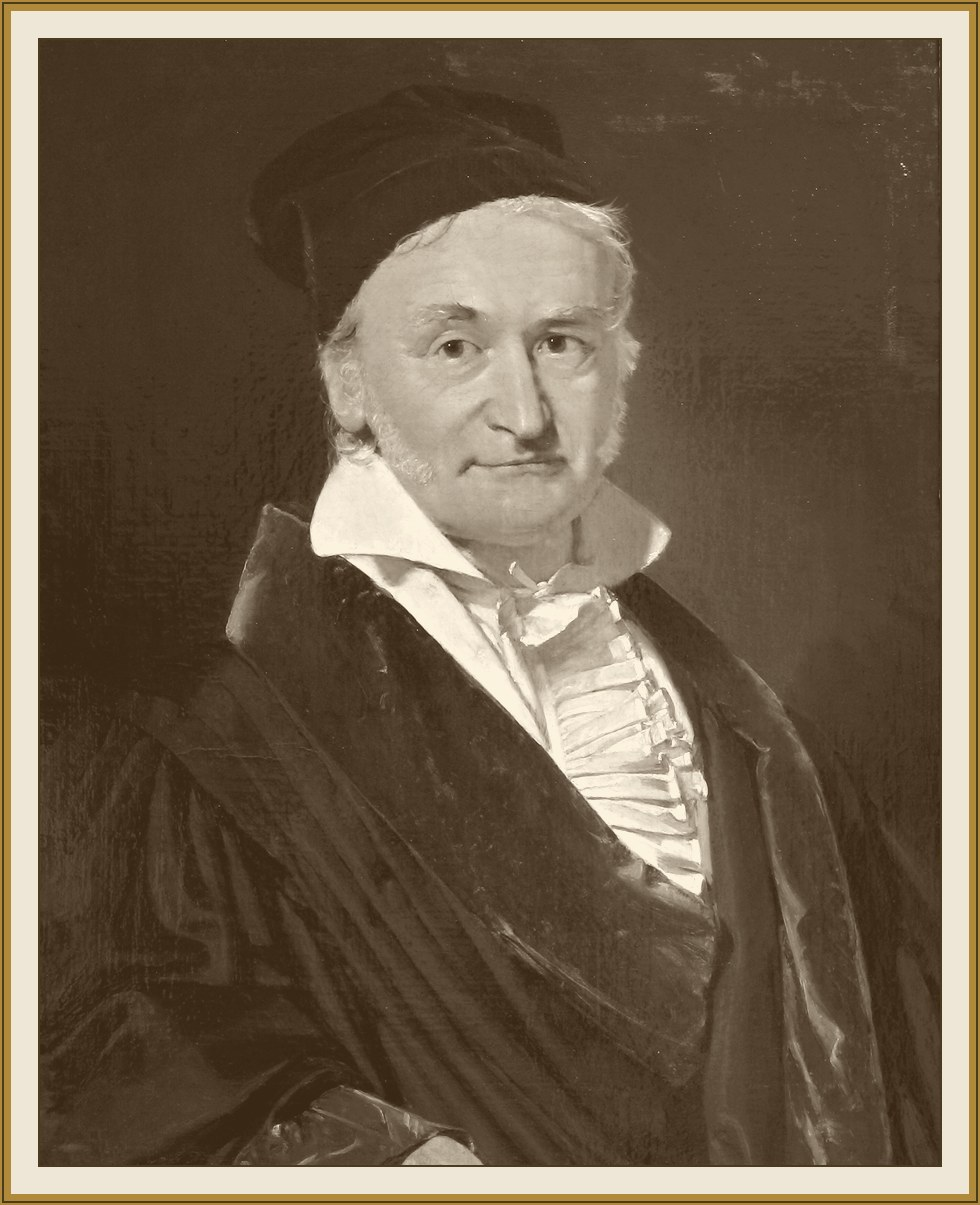
\includegraphics[keepaspectratio]{images/session-03-gauss.jpg}}

\textbf{Carl Friedrich Gauss} · \textbf{1777--1855}

Least squares, and the theorem that says when it is the best you can do.

{Christian Albrecht Jensen, 1840. Public domain, via Wikimedia Commons.}

\end{qmibplate}

\begin{qmibplate}

\pandocbounded{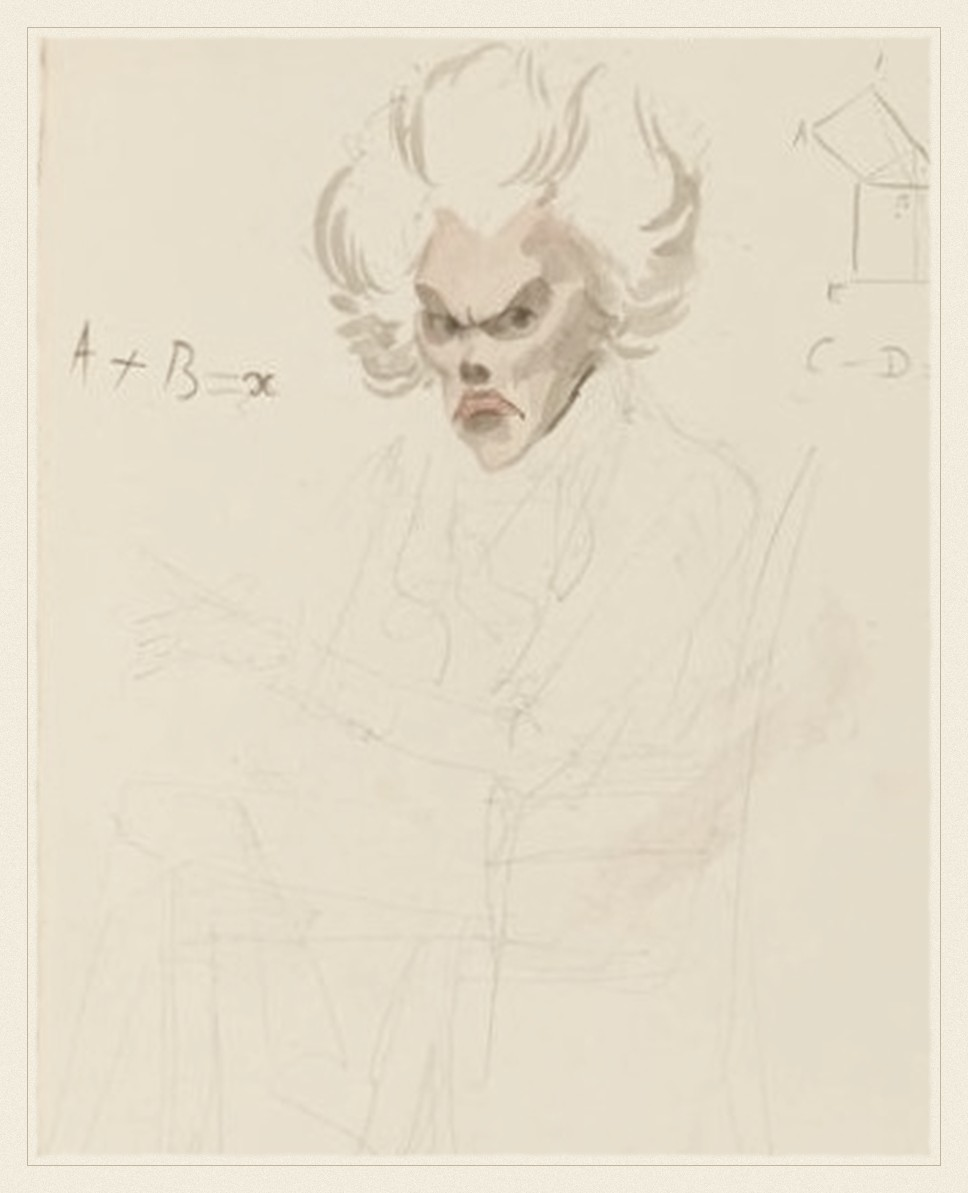
\includegraphics[keepaspectratio]{images/session-03-legendre.jpg}}

\textbf{Adrien-Marie Legendre} · \textbf{1752--1833}

Published least squares first, in 1805. This caricature is the only
likeness of him known to exist.

{Julien-Léopold Boilly, undated. Public domain, via Wikimedia Commons.}

\end{qmibplate}

\end{qmibplate}

Set the problem up. You have \(n\) observations, a response \(y\), and a
matrix \(X\) holding a column of ones and \(p-1\) predictors. You want
coefficients \(\beta\) such that \(X\beta\) is close to \(y\). Least
squares defines ``close'' as the sum of squared vertical distances, and
chooses

\[
\hat\beta \;=\; \arg\min_{\beta} \; \lVert y - X\beta \rVert^2 .
\]

Squared, rather than absolute, distance is worth pausing on, because the
choice is not obvious and it has consequences you will meet later in the
chapter. Squaring makes the objective differentiable everywhere, which
is what delivers the closed-form solution below; it also makes the
fitted values a \emph{linear} function of \(y\), which is what makes the
whole diagnostic apparatus possible. The price is that squaring gives a
doubled error four times the weight of a single one, so least squares is
structurally sensitive to observations far from the line. Every
technique in this chapter for finding influential points is, in a sense,
paying off the debt incurred by that square.

Differentiating and setting to zero gives the \emph{normal equations}
\(X^{\top}X\beta = X^{\top}y\), whose solution --- whenever
\(X^{\top}X\) can be inverted --- is

\[
\hat\beta \;=\; (X^{\top}X)^{-1} X^{\top} y .
\]

Every equation in this chapter is something you can execute, and
executing it is the fastest way to find out whether you have understood
what it claims. The normal equations are the first: solve them by hand
and the answer must be, to floating-point precision, whatever
\texttt{statsmodels} returns.

\phantomsection\label{check-ols}
\begin{Shaded}
\begin{Highlighting}[]
\ImportTok{import}\NormalTok{ sys, warnings}
\NormalTok{sys.path.insert(}\DecValTok{0}\NormalTok{, }\StringTok{"../slides"}\NormalTok{)}\OperatorTok{;}\NormalTok{ sys.path.insert(}\DecValTok{0}\NormalTok{, }\StringTok{".."}\NormalTok{)}
\NormalTok{warnings.filterwarnings(}\StringTok{"ignore"}\NormalTok{)}
\ImportTok{from}\NormalTok{ plotstyle }\ImportTok{import}\NormalTok{ setup, CL}
\NormalTok{plt }\OperatorTok{=}\NormalTok{ setup()}

\ImportTok{import}\NormalTok{ numpy }\ImportTok{as}\NormalTok{ np, pandas }\ImportTok{as}\NormalTok{ pd, statsmodels.api }\ImportTok{as}\NormalTok{ sm, qmib}

\NormalTok{d }\OperatorTok{=}\NormalTok{ (qmib.load(}\StringTok{"core"}\NormalTok{)}
\NormalTok{     .dropna(subset}\OperatorTok{=}\NormalTok{[}\StringTok{"gdp\_pc\_eur"}\NormalTok{, }\StringTok{"productivity\_idx"}\NormalTok{])}
\NormalTok{     .reset\_index(drop}\OperatorTok{=}\VariableTok{True}\NormalTok{))}
\NormalTok{X }\OperatorTok{=}\NormalTok{ sm.add\_constant(d[}\StringTok{"productivity\_idx"}\NormalTok{]).to\_numpy()}
\NormalTok{y }\OperatorTok{=}\NormalTok{ d[}\StringTok{"gdp\_pc\_eur"}\NormalTok{].to\_numpy()}

\CommentTok{\# beta\_hat = (X\textquotesingle{}X)\^{}{-}1 X\textquotesingle{}y — written as solve(), never as inv(), because}
\CommentTok{\# inverting a matrix to multiply it by a vector is slower and less stable.}
\NormalTok{beta\_hand }\OperatorTok{=}\NormalTok{ np.linalg.solve(X.T }\OperatorTok{@}\NormalTok{ X, X.T }\OperatorTok{@}\NormalTok{ y)}
\NormalTok{beta\_sm }\OperatorTok{=}\NormalTok{ sm.OLS(y, X).fit().params}

\BuiltInTok{print}\NormalTok{(}\StringTok{"by hand      "}\NormalTok{, np.}\BuiltInTok{round}\NormalTok{(beta\_hand, }\DecValTok{6}\NormalTok{))}
\BuiltInTok{print}\NormalTok{(}\StringTok{"statsmodels  "}\NormalTok{, np.}\BuiltInTok{round}\NormalTok{(beta\_sm, }\DecValTok{6}\NormalTok{))}
\BuiltInTok{print}\NormalTok{(}\StringTok{"agree to     "}\NormalTok{, }\SpecialStringTok{f"}\SpecialCharTok{\{}\NormalTok{np}\SpecialCharTok{.}\BuiltInTok{abs}\NormalTok{(beta\_hand }\OperatorTok{{-}}\NormalTok{ beta\_sm)}\SpecialCharTok{.}\BuiltInTok{max}\NormalTok{()}\SpecialCharTok{:.2e\}}\SpecialStringTok{"}\NormalTok{)}
\end{Highlighting}
\end{Shaded}

\begin{verbatim}
by hand       [-86118.084706   1111.257354]
statsmodels   [-86118.084706   1111.257354]
agree to      2.49e-09
\end{verbatim}

That is an algebraic fact. It requires no assumption about the world, no
probability, no error term. Feed it any numbers and it returns
coefficients. This is exactly why diagnostics are necessary: \textbf{the
formula never refuses.} It has no way to tell you that the relationship
is curved, that one country is dragging the whole line, or that the
standard errors it reports are fiction. It returns the same confident
four decimal places either way.

The statistical content arrives only when you attach a model,

\[
y \;=\; X\beta + \varepsilon ,
\]

and make claims about \(\varepsilon\). The Gauss--Markov theorem says
that if the model is correctly specified, if
\(\operatorname{E}[\varepsilon \mid X] = 0\), and if the errors have
constant variance and are mutually uncorrelated, then \(\hat\beta\) is
the Best Linear Unbiased Estimator: no other estimator that is both
linear in \(y\) and unbiased has smaller variance. Note what is
\emph{not} on that list. Normality is not required for Gauss--Markov. It
is required for something else --- the exactness of the \(t\) and \(F\)
distributions in small samples --- and confusing the two is one of the
most common errors in applied work.

The word ``regression'' itself arrived later and by accident. Francis
Galton, studying the heights of parents and children, found that tall
parents had children who were tall but \emph{less} tall, and called this
``regression towards mediocrity'' (\citeproc{ref-galton1886}{Galton
1886}). He was naming a substantive biological phenomenon. The name
stuck to the statistical method he had used to find it, which is why a
technique for fitting conditional means is called by a word that means
moving backwards.

\begin{qmibarchive}

\textbf{From the archive · Galton, 1886}

Galton's claim was about heredity, but the phenomenon is general and it
is not a fact about biology: it follows from the arithmetic of an
imperfect correlation. Whenever two measurements of the same thing are
less than perfectly correlated, the extremes of the first are, on
average, less extreme in the second --- not because anything pulled them
back, but because part of what made them extreme was noise, and noise
does not repeat.

It is worth seeing this happen in the data this book uses. These are
fixtures rather than observations, which for once does not weaken the
demonstration: regression towards the mean is a consequence of imperfect
correlation, not of economics, so it turns up in any series where this
year predicts next year imperfectly --- generated or observed. Take each
country's productivity in a given year, expressed as a deviation from
that year's cross-country average, and ask what that deviation looks
like the following year.

\begin{Shaded}
\begin{Highlighting}[]
\ImportTok{import}\NormalTok{ sys, warnings}
\NormalTok{sys.path.insert(}\DecValTok{0}\NormalTok{, }\StringTok{"../slides"}\NormalTok{)}\OperatorTok{;}\NormalTok{ sys.path.insert(}\DecValTok{0}\NormalTok{, }\StringTok{".."}\NormalTok{)}
\NormalTok{warnings.filterwarnings(}\StringTok{"ignore"}\NormalTok{)}
\ImportTok{from}\NormalTok{ plotstyle }\ImportTok{import}\NormalTok{ setup, CL}
\NormalTok{plt }\OperatorTok{=}\NormalTok{ setup()}

\ImportTok{import}\NormalTok{ qmib, numpy }\ImportTok{as}\NormalTok{ np, pandas }\ImportTok{as}\NormalTok{ pd}

\NormalTok{d }\OperatorTok{=}\NormalTok{ (qmib.load(}\StringTok{"core"}\NormalTok{).dropna(subset}\OperatorTok{=}\NormalTok{[}\StringTok{"productivity\_idx"}\NormalTok{])}
\NormalTok{     .sort\_values([}\StringTok{"geo"}\NormalTok{, }\StringTok{"time"}\NormalTok{]))}
\NormalTok{d[}\StringTok{"next"}\NormalTok{] }\OperatorTok{=}\NormalTok{ d.groupby(}\StringTok{"geo"}\NormalTok{)[}\StringTok{"productivity\_idx"}\NormalTok{].shift(}\OperatorTok{{-}}\DecValTok{1}\NormalTok{)}
\NormalTok{pairs }\OperatorTok{=}\NormalTok{ d.dropna(subset}\OperatorTok{=}\NormalTok{[}\StringTok{"next"}\NormalTok{]).copy()}

\CommentTok{\# Deviation from the cross{-}country mean, this year and the next.}
\NormalTok{pairs[}\StringTok{"dev"}\NormalTok{] }\OperatorTok{=}\NormalTok{ pairs[}\StringTok{"productivity\_idx"}\NormalTok{] }\OperatorTok{{-}}\NormalTok{ pairs.groupby(}\StringTok{"time"}\NormalTok{)[}\StringTok{"productivity\_idx"}\NormalTok{].transform(}\StringTok{"mean"}\NormalTok{)}
\NormalTok{pairs[}\StringTok{"dev\_next"}\NormalTok{] }\OperatorTok{=}\NormalTok{ pairs[}\StringTok{"next"}\NormalTok{] }\OperatorTok{{-}}\NormalTok{ pairs.groupby(}\StringTok{"time"}\NormalTok{)[}\StringTok{"next"}\NormalTok{].transform(}\StringTok{"mean"}\NormalTok{)}

\NormalTok{slope, intercept }\OperatorTok{=}\NormalTok{ np.polyfit(pairs[}\StringTok{"dev"}\NormalTok{], pairs[}\StringTok{"dev\_next"}\NormalTok{], }\DecValTok{1}\NormalTok{)}

\NormalTok{fig, ax }\OperatorTok{=}\NormalTok{ plt.subplots(figsize}\OperatorTok{=}\NormalTok{(}\FloatTok{6.0}\NormalTok{, }\FloatTok{4.6}\NormalTok{))}
\NormalTok{lim }\OperatorTok{=}\NormalTok{ np.array([pairs[}\StringTok{"dev"}\NormalTok{].}\BuiltInTok{min}\NormalTok{() }\OperatorTok{*} \FloatTok{1.05}\NormalTok{, pairs[}\StringTok{"dev"}\NormalTok{].}\BuiltInTok{max}\NormalTok{() }\OperatorTok{*} \FloatTok{1.05}\NormalTok{])}
\NormalTok{ax.plot(lim, lim, ls}\OperatorTok{=}\StringTok{":"}\NormalTok{, lw}\OperatorTok{=}\FloatTok{1.3}\NormalTok{, color}\OperatorTok{=}\NormalTok{CL.muted, label}\OperatorTok{=}\StringTok{"no regression to the mean"}\NormalTok{)}
\NormalTok{ax.plot(lim, intercept }\OperatorTok{+}\NormalTok{ slope }\OperatorTok{*}\NormalTok{ lim, lw}\OperatorTok{=}\DecValTok{2}\NormalTok{, color}\OperatorTok{=}\NormalTok{CL.warn,}
\NormalTok{        label}\OperatorTok{=}\SpecialStringTok{f"fitted, slope = }\SpecialCharTok{\{}\NormalTok{slope}\SpecialCharTok{:.2f\}}\SpecialStringTok{"}\NormalTok{)}
\NormalTok{ax.scatter(pairs[}\StringTok{"dev"}\NormalTok{], pairs[}\StringTok{"dev\_next"}\NormalTok{], s}\OperatorTok{=}\DecValTok{15}\NormalTok{, color}\OperatorTok{=}\NormalTok{CL.accent,}
\NormalTok{           alpha}\OperatorTok{=}\FloatTok{0.5}\NormalTok{, edgecolor}\OperatorTok{=}\StringTok{"none"}\NormalTok{, zorder}\OperatorTok{=}\DecValTok{3}\NormalTok{)}
\NormalTok{ax.axhline(}\DecValTok{0}\NormalTok{, color}\OperatorTok{=}\NormalTok{CL.line, lw}\OperatorTok{=}\DecValTok{1}\NormalTok{, zorder}\OperatorTok{=}\DecValTok{1}\NormalTok{)}\OperatorTok{;}\NormalTok{ ax.axvline(}\DecValTok{0}\NormalTok{, color}\OperatorTok{=}\NormalTok{CL.line, lw}\OperatorTok{=}\DecValTok{1}\NormalTok{, zorder}\OperatorTok{=}\DecValTok{1}\NormalTok{)}
\NormalTok{ax.set\_xlabel(}\StringTok{"deviation from the mean, year $t$"}\NormalTok{)}
\NormalTok{ax.set\_ylabel(}\StringTok{"deviation from the mean, year $t+1$"}\NormalTok{)}
\NormalTok{ax.legend(frameon}\OperatorTok{=}\VariableTok{False}\NormalTok{, fontsize}\OperatorTok{=}\FloatTok{8.5}\NormalTok{, loc}\OperatorTok{=}\StringTok{"upper left"}\NormalTok{)}
\NormalTok{fig.tight\_layout()}
\end{Highlighting}
\end{Shaded}

\begin{figure}[htbp]

\centering{

\pandocbounded{
\includegraphics[keepaspectratio]{session-03_files/figure-pdf/fig-galton-output-1.png}}

}

\caption{\label{fig-galton}Regression towards the mean in the course
fixtures, 2010--2024. Each point is one country-year: its deviation from
the cross-country average that year, against its deviation the next. A
slope below 1 is Galton's phenomenon. The values are generated, not
observed --- but the phenomenon is a property of imperfect correlation,
so it appears here for the same reason it appears in real data.}

\end{figure}%

The dotted line is what perfect persistence would look like: a country
as far above average next year as it was this year. The fitted line is
flatter. The most productive decile keeps about six-sevenths of its lead
from one year to the next, and the least productive recovers by a
comparable amount --- with nothing whatever having been done to either.

The warning Galton's contemporaries missed is the one to carry forward.
If you select the extremes and then measure them again, they will
improve, and the improvement will look like the effect of whatever you
did in between. Chapter 10 returns to this as a threat to causal
inference, where it has a name: regression to the mean is the reason a
single-group before-and-after comparison is not evidence.

\end{qmibarchive}

\section{Adequacy, validity,
robustness}\label{adequacy-validity-robustness}

These three words get used loosely and they are not synonyms. The
distinction organises everything that follows.

\begin{qmibdefinition}

{\textbf{Adequacy}} --- whether the model describes the data you
actually have. An adequate model leaves residuals with no remaining
structure: nothing in what is left over could have been used to predict
\(y\) better. Adequacy is assessed against the sample, and it is mostly
a question you answer with plots.

\end{qmibdefinition}

\begin{qmibdefinition}

{\textbf{Validity}} --- whether the inferences you draw from the model
are warranted: whether the standard errors, confidence intervals and
\(p\)-values mean what they claim. A model can be adequate and its
inference invalid, most commonly because the errors are heteroscedastic
or dependent. Validity is a question about the \emph{sampling
distribution}, not about fit.

\end{qmibdefinition}

\begin{qmibdefinition}

{\textbf{Robustness}} --- whether your conclusions survive reasonable
changes to the specification, the sample or the estimator. A robust
finding is one that does not depend on a single influential observation,
one functional form, or one way of computing standard errors. Robustness
is a question about \emph{stability}.

\end{qmibdefinition}

Keeping them apart tells you what a given failure actually costs, and
this is the part most often got wrong. The four classical assumptions do
not all protect the same thing:

\begin{longtable}[]{@{}
  >{\raggedright\arraybackslash}p{(\linewidth - 6\tabcolsep) * \real{0.2500}}
  >{\raggedright\arraybackslash}p{(\linewidth - 6\tabcolsep) * \real{0.2500}}
  >{\raggedright\arraybackslash}p{(\linewidth - 6\tabcolsep) * \real{0.2500}}
  >{\raggedright\arraybackslash}p{(\linewidth - 6\tabcolsep) * \real{0.2500}}@{}}
\toprule\noalign{}
\begin{minipage}[b]{\linewidth}\raggedright
If this fails
\end{minipage} & \begin{minipage}[b]{\linewidth}\raggedright
\(\hat\beta\) is
\end{minipage} & \begin{minipage}[b]{\linewidth}\raggedright
Standard errors are
\end{minipage} & \begin{minipage}[b]{\linewidth}\raggedright
So the damage is to
\end{minipage} \\
\midrule\noalign{}
\endhead
\bottomrule\noalign{}
\endlastfoot
Correct specification & \textbf{biased} & meaningless & the estimate
itself \\
Constant variance & unbiased & \textbf{wrong} & validity only \\
Independent errors & unbiased & \textbf{wrong}, usually far too small &
validity only \\
Normal errors & unbiased & fine in large samples & almost nothing, if
\(n\) is large \\
\end{longtable}

Read the table twice. Only the first row damages the coefficient. Rows
two and three leave your estimate untouched and destroy your uncertainty
--- you have the right number with the wrong error bar, which matters
enormously if the question is whether an effect can be distinguished
from zero. Row four, the assumption students worry about most, is the
one that matters least.

A model with \(R^2 = 0.95\) can fail all of it. This is not
hypothetical: Anscombe's four datasets share, to two decimal places, the
same means, variances, correlation, regression line and \(R^2\), and
they are utterly different (\citeproc{ref-anscombe1973}{Anscombe 1973}).

\begin{Shaded}
\begin{Highlighting}[]
\ImportTok{import}\NormalTok{ sys, warnings}
\NormalTok{sys.path.insert(}\DecValTok{0}\NormalTok{, }\StringTok{"../slides"}\NormalTok{)}\OperatorTok{;}\NormalTok{ sys.path.insert(}\DecValTok{0}\NormalTok{, }\StringTok{".."}\NormalTok{)}
\NormalTok{warnings.filterwarnings(}\StringTok{"ignore"}\NormalTok{)}
\ImportTok{from}\NormalTok{ plotstyle }\ImportTok{import}\NormalTok{ setup, CL}
\NormalTok{plt }\OperatorTok{=}\NormalTok{ setup()}
\ImportTok{import}\NormalTok{ numpy }\ImportTok{as}\NormalTok{ np}

\NormalTok{x1 }\OperatorTok{=}\NormalTok{ [}\DecValTok{10}\NormalTok{, }\DecValTok{8}\NormalTok{, }\DecValTok{13}\NormalTok{, }\DecValTok{9}\NormalTok{, }\DecValTok{11}\NormalTok{, }\DecValTok{14}\NormalTok{, }\DecValTok{6}\NormalTok{, }\DecValTok{4}\NormalTok{, }\DecValTok{12}\NormalTok{, }\DecValTok{7}\NormalTok{, }\DecValTok{5}\NormalTok{]}
\NormalTok{quartet }\OperatorTok{=}\NormalTok{ \{}
    \StringTok{"I — the line is right"}\NormalTok{:        (x1, [}\FloatTok{8.04}\NormalTok{, }\FloatTok{6.95}\NormalTok{, }\FloatTok{7.58}\NormalTok{, }\FloatTok{8.81}\NormalTok{, }\FloatTok{8.33}\NormalTok{, }\FloatTok{9.96}\NormalTok{, }\FloatTok{7.24}\NormalTok{, }\FloatTok{4.26}\NormalTok{, }\FloatTok{10.84}\NormalTok{, }\FloatTok{4.82}\NormalTok{, }\FloatTok{5.68}\NormalTok{]),}
    \StringTok{"II — the relation is curved"}\NormalTok{:  (x1, [}\FloatTok{9.14}\NormalTok{, }\FloatTok{8.14}\NormalTok{, }\FloatTok{8.74}\NormalTok{, }\FloatTok{8.77}\NormalTok{, }\FloatTok{9.26}\NormalTok{, }\FloatTok{8.10}\NormalTok{, }\FloatTok{6.13}\NormalTok{, }\FloatTok{3.10}\NormalTok{, }\FloatTok{9.13}\NormalTok{, }\FloatTok{7.26}\NormalTok{, }\FloatTok{4.74}\NormalTok{]),}
    \StringTok{"III — one outlier tilts it"}\NormalTok{:   (x1, [}\FloatTok{7.46}\NormalTok{, }\FloatTok{6.77}\NormalTok{, }\FloatTok{12.74}\NormalTok{, }\FloatTok{7.11}\NormalTok{, }\FloatTok{7.81}\NormalTok{, }\FloatTok{8.84}\NormalTok{, }\FloatTok{6.08}\NormalTok{, }\FloatTok{5.39}\NormalTok{, }\FloatTok{8.15}\NormalTok{, }\FloatTok{6.42}\NormalTok{, }\FloatTok{5.73}\NormalTok{]),}
    \StringTok{"IV — one point defines it"}\NormalTok{:    ([}\DecValTok{8}\NormalTok{]}\OperatorTok{*}\DecValTok{10} \OperatorTok{+}\NormalTok{ [}\DecValTok{19}\NormalTok{], [}\FloatTok{6.58}\NormalTok{, }\FloatTok{5.76}\NormalTok{, }\FloatTok{7.71}\NormalTok{, }\FloatTok{8.84}\NormalTok{, }\FloatTok{8.47}\NormalTok{, }\FloatTok{7.04}\NormalTok{, }\FloatTok{5.25}\NormalTok{, }\FloatTok{5.56}\NormalTok{, }\FloatTok{7.91}\NormalTok{, }\FloatTok{6.89}\NormalTok{, }\FloatTok{12.50}\NormalTok{]),}
\NormalTok{\}}

\NormalTok{fig, axes }\OperatorTok{=}\NormalTok{ plt.subplots(}\DecValTok{2}\NormalTok{, }\DecValTok{2}\NormalTok{, figsize}\OperatorTok{=}\NormalTok{(}\FloatTok{8.6}\NormalTok{, }\FloatTok{6.4}\NormalTok{), sharex}\OperatorTok{=}\VariableTok{True}\NormalTok{, sharey}\OperatorTok{=}\VariableTok{True}\NormalTok{)}
\ControlFlowTok{for}\NormalTok{ ax, (name, (x, y)) }\KeywordTok{in} \BuiltInTok{zip}\NormalTok{(axes.ravel(), quartet.items()):}
\NormalTok{    x, y }\OperatorTok{=}\NormalTok{ np.asarray(x, }\BuiltInTok{float}\NormalTok{), np.asarray(y, }\BuiltInTok{float}\NormalTok{)}
\NormalTok{    b }\OperatorTok{=}\NormalTok{ np.polyfit(x, y, }\DecValTok{1}\NormalTok{)}
\NormalTok{    gx }\OperatorTok{=}\NormalTok{ np.linspace(}\DecValTok{2}\NormalTok{, }\DecValTok{20}\NormalTok{, }\DecValTok{50}\NormalTok{)}
\NormalTok{    ax.plot(gx, np.polyval(b, gx), color}\OperatorTok{=}\NormalTok{CL.warn, lw}\OperatorTok{=}\FloatTok{1.6}\NormalTok{, zorder}\OperatorTok{=}\DecValTok{2}\NormalTok{)}
\NormalTok{    ax.scatter(x, y, s}\OperatorTok{=}\DecValTok{36}\NormalTok{, color}\OperatorTok{=}\NormalTok{CL.accent, zorder}\OperatorTok{=}\DecValTok{3}\NormalTok{, edgecolor}\OperatorTok{=}\StringTok{"white"}\NormalTok{, linewidth}\OperatorTok{=}\FloatTok{0.8}\NormalTok{)}
\NormalTok{    r2 }\OperatorTok{=}\NormalTok{ np.corrcoef(x, y)[}\DecValTok{0}\NormalTok{, }\DecValTok{1}\NormalTok{] }\OperatorTok{**} \DecValTok{2}
\NormalTok{    ax.set\_title(name, fontsize}\OperatorTok{=}\DecValTok{10}\NormalTok{, loc}\OperatorTok{=}\StringTok{"left"}\NormalTok{, color}\OperatorTok{=}\NormalTok{CL.ink)}
\NormalTok{    ax.text(}\FloatTok{0.97}\NormalTok{, }\FloatTok{0.06}\NormalTok{, }\SpecialStringTok{f"$R\^{}2=}\SpecialCharTok{\{}\NormalTok{r2}\SpecialCharTok{:.2f\}}\SpecialStringTok{$"}\NormalTok{, transform}\OperatorTok{=}\NormalTok{ax.transAxes,}
\NormalTok{            ha}\OperatorTok{=}\StringTok{"right"}\NormalTok{, fontsize}\OperatorTok{=}\DecValTok{9}\NormalTok{, color}\OperatorTok{=}\NormalTok{CL.muted)}
\NormalTok{    ax.set\_xlim(}\DecValTok{2}\NormalTok{, }\DecValTok{20}\NormalTok{)}\OperatorTok{;}\NormalTok{ ax.set\_ylim(}\DecValTok{2}\NormalTok{, }\DecValTok{14}\NormalTok{)}
\NormalTok{fig.tight\_layout()}
\end{Highlighting}
\end{Shaded}

\begin{figure}[htbp]

\centering{

\pandocbounded{
\includegraphics[keepaspectratio]{session-03_files/figure-pdf/fig-anscombe-output-1.png}}

}

\caption{\label{fig-anscombe}Anscombe's quartet. Identical means,
variances, correlations, fitted lines and \(R^2\) --- and only the first
is a dataset the line describes. Data from Anscombe
(\citeproc{ref-anscombe1973}{1973}), Table 1.}

\end{figure}%

Every one of those four panels reports \(R^2 = 0.67\) and the same
fitted line. Only in the first is that line a description of the data.
In the second the relationship is deterministic and curved --- the model
is not wrong about the strength of the association so much as wrong
about its \emph{shape}, and no amount of extra data will fix it, because
more observations of a parabola still make a parabola. In the third a
single aberrant point has tilted a line that would otherwise pass almost
exactly through the rest; delete it and both the slope and the residual
variance change sharply. In the fourth every \(x\) but one is identical,
so the slope is determined entirely by one observation: delete it and
the slope is not merely different, it is undefined, because
\(X^{\top}X\) becomes singular.

Anscombe's point was not that summary statistics are useless. It was
that they are \emph{insufficient}, and that the missing information is
available for the cost of a plot.

\section{What the residual knows}\label{what-the-residual-knows}

Write \(\hat y = X\hat\beta\). Substituting the estimator,

\[
\hat y \;=\; X(X^{\top}X)^{-1}X^{\top} y \;=\; Hy ,
\]

where \(H = X(X^{\top}X)^{-1}X^{\top}\) is the \emph{hat matrix} --- so
named because it puts the hat on \(y\). Geometrically it is the
orthogonal projection onto the column space of \(X\): it takes the
\(n\)-dimensional vector of observations and casts its shadow onto the
\(p\)-dimensional subspace the model can reach. That picture is worth
holding, because it makes the next two properties obvious rather than
algebraic. \(H\) is symmetric (\(H = H^{\top}\)) and idempotent
(\(HH = H\)) --- projecting a shadow again does nothing, since it is
already flat.

The residual vector is what the projection could not reach,

\[
e \;=\; y - \hat y \;=\; (I - H)\, y ,
\]

and it is orthogonal to every column of \(X\) by construction. That
orthogonality is the reason residual plots are informative \emph{and}
the reason they can mislead: \(e\) is guaranteed to be uncorrelated with
each predictor whether or not the model is right, so a flat residual
plot against \(x\) is not evidence of anything. What is \emph{not}
guaranteed is the absence of non-linear structure, which is exactly what
you are looking for.

Now the consequence that governs every diagnostic below. If
\(\operatorname{Var}(\varepsilon) = \sigma^2 I\), then

\[
\operatorname{Var}(e) \;=\; \sigma^{2}(I - H),
\qquad\text{so}\qquad
\operatorname{Var}(e_i) \;=\; \sigma^{2}\,(1 - h_{ii}).
\]

\textbf{The residuals do not have constant variance even when the errors
do.} An observation with large \(h_{ii}\) has a residual squeezed
towards zero as a matter of arithmetic, not because the model fits it
well. The most dangerous points therefore look like the best-behaved
ones. This is why raw residuals are the wrong thing to plot, and why
everything below is built on the \emph{standardised} residual

\[
r_i \;=\; \frac{e_i}{s\sqrt{1 - h_{ii}}},
\qquad s^2 = \frac{e^{\top}e}{n-p},
\]

which divides out the arithmetic squeeze and restores comparability.
Plotting \(r_i\) against \(\hat y_i\) is the single most informative
diagnostic there is (\citeproc{ref-anscombe1963}{Anscombe and Tukey
1963}). Under an adequate model the cloud is structureless: flat,
centred on zero, of even width. Curvature means the functional form is
wrong. A widening fan means the variance is not constant. Both are
visible instantly and neither is visible in \(R^2\).

Why plot against \(\hat y\) rather than against \(x\)? Because with
several predictors there is no single \(x\) to use, and \(\hat y\) is
the one-dimensional summary the model actually commits to. It is also
the axis along which heteroscedasticity usually manifests, since the
spread of an economic quantity so often scales with its level.

\begin{Shaded}
\begin{Highlighting}[]
\ImportTok{import}\NormalTok{ pandas }\ImportTok{as}\NormalTok{ pd, statsmodels.api }\ImportTok{as}\NormalTok{ sm}
\ImportTok{from}\NormalTok{ statsmodels.nonparametric.smoothers\_lowess }\ImportTok{import}\NormalTok{ lowess}
\ImportTok{import}\NormalTok{ qmib}

\NormalTok{d }\OperatorTok{=}\NormalTok{ qmib.load(}\StringTok{"core"}\NormalTok{).dropna(subset}\OperatorTok{=}\NormalTok{[}\StringTok{"gdp\_pc\_eur"}\NormalTok{, }\StringTok{"productivity\_idx"}\NormalTok{]).reset\_index(drop}\OperatorTok{=}\VariableTok{True}\NormalTok{)}
\NormalTok{X }\OperatorTok{=}\NormalTok{ sm.add\_constant(d[}\StringTok{"productivity\_idx"}\NormalTok{])}
\NormalTok{model }\OperatorTok{=}\NormalTok{ sm.OLS(d[}\StringTok{"gdp\_pc\_eur"}\NormalTok{], X).fit()}
\NormalTok{infl }\OperatorTok{=}\NormalTok{ model.get\_influence()}
\NormalTok{std\_resid }\OperatorTok{=}\NormalTok{ infl.resid\_studentized\_internal}
\NormalTok{fitted }\OperatorTok{=}\NormalTok{ model.fittedvalues.values}

\NormalTok{fig, (ax1, ax2) }\OperatorTok{=}\NormalTok{ plt.subplots(}\DecValTok{1}\NormalTok{, }\DecValTok{2}\NormalTok{, figsize}\OperatorTok{=}\NormalTok{(}\FloatTok{9.2}\NormalTok{, }\FloatTok{3.9}\NormalTok{))}

\NormalTok{ax1.axhline(}\DecValTok{0}\NormalTok{, color}\OperatorTok{=}\NormalTok{CL.muted, lw}\OperatorTok{=}\DecValTok{1}\NormalTok{, zorder}\OperatorTok{=}\DecValTok{1}\NormalTok{)}
\NormalTok{ax1.scatter(fitted, std\_resid, s}\OperatorTok{=}\DecValTok{16}\NormalTok{, color}\OperatorTok{=}\NormalTok{CL.accent, alpha}\OperatorTok{=}\FloatTok{0.5}\NormalTok{, edgecolor}\OperatorTok{=}\StringTok{"none"}\NormalTok{, zorder}\OperatorTok{=}\DecValTok{3}\NormalTok{)}
\NormalTok{sm\_line }\OperatorTok{=}\NormalTok{ lowess(std\_resid, fitted, frac}\OperatorTok{=}\FloatTok{0.5}\NormalTok{, return\_sorted}\OperatorTok{=}\VariableTok{True}\NormalTok{)}
\NormalTok{ax1.plot(sm\_line[:, }\DecValTok{0}\NormalTok{], sm\_line[:, }\DecValTok{1}\NormalTok{], color}\OperatorTok{=}\NormalTok{CL.warn, lw}\OperatorTok{=}\FloatTok{1.9}\NormalTok{, zorder}\OperatorTok{=}\DecValTok{4}\NormalTok{)}
\NormalTok{ax1.set\_xlabel(}\StringTok{"fitted value"}\NormalTok{)}\OperatorTok{;}\NormalTok{ ax1.set\_ylabel(}\StringTok{"standardised residual"}\NormalTok{)}
\NormalTok{ax1.set\_title(}\StringTok{"Residuals vs fitted"}\NormalTok{, fontsize}\OperatorTok{=}\DecValTok{10}\NormalTok{, loc}\OperatorTok{=}\StringTok{"left"}\NormalTok{)}

\NormalTok{root }\OperatorTok{=}\NormalTok{ np.sqrt(np.}\BuiltInTok{abs}\NormalTok{(std\_resid))}
\NormalTok{ax2.scatter(fitted, root, s}\OperatorTok{=}\DecValTok{16}\NormalTok{, color}\OperatorTok{=}\NormalTok{CL.accent, alpha}\OperatorTok{=}\FloatTok{0.5}\NormalTok{, edgecolor}\OperatorTok{=}\StringTok{"none"}\NormalTok{, zorder}\OperatorTok{=}\DecValTok{3}\NormalTok{)}
\NormalTok{sm2 }\OperatorTok{=}\NormalTok{ lowess(root, fitted, frac}\OperatorTok{=}\FloatTok{0.5}\NormalTok{, return\_sorted}\OperatorTok{=}\VariableTok{True}\NormalTok{)}
\NormalTok{ax2.plot(sm2[:, }\DecValTok{0}\NormalTok{], sm2[:, }\DecValTok{1}\NormalTok{], color}\OperatorTok{=}\NormalTok{CL.warn, lw}\OperatorTok{=}\FloatTok{1.9}\NormalTok{, zorder}\OperatorTok{=}\DecValTok{4}\NormalTok{)}
\NormalTok{ax2.set\_xlabel(}\StringTok{"fitted value"}\NormalTok{)}\OperatorTok{;}\NormalTok{ ax2.set\_ylabel(}\VerbatimStringTok{r"}\DecValTok{$\textbackslash{}s}\VerbatimStringTok{qrt\{}\ControlFlowTok{|}\CharTok{\textbackslash{},}\VerbatimStringTok{r\_i}\CharTok{\textbackslash{},}\ControlFlowTok{|}\VerbatimStringTok{\}}\DecValTok{$}\VerbatimStringTok{"}\NormalTok{)}
\NormalTok{ax2.set\_title(}\StringTok{"Scale–location"}\NormalTok{, fontsize}\OperatorTok{=}\DecValTok{10}\NormalTok{, loc}\OperatorTok{=}\StringTok{"left"}\NormalTok{)}

\NormalTok{fig.tight\_layout()}
\end{Highlighting}
\end{Shaded}

\begin{figure}[htbp]

\centering{

\pandocbounded{
\includegraphics[keepaspectratio]{session-03_files/figure-pdf/fig-diagnostics-output-1.png}}

}

\caption{\label{fig-diagnostics}Diagnostics for GDP per capita on the
productivity index --- the regression Session 02 fitted. Left:
standardised residuals against fitted values, with a LOWESS smoother
(\citeproc{ref-cleveland1979}{Cleveland 1979}). Right: the
scale--location plot, which removes the sign so that changing spread is
easier to see.}

\end{figure}%

Read Figure~\ref{fig-diagnostics} the way a referee would, which means
saying what you looked for before saying what you saw. In the left panel
you are looking for curvature in the smoother and for a cloud of even
vertical width; the smoother drifts rather than sitting flat, which says
a straight line is missing some of the shape of the relationship between
productivity and income. In the right panel you are looking for a trend,
and there is one: the spread of the residuals grows with the fitted
value: the wealthier the country-year, the wider the spread of what the
model gets wrong. Whether that is true of Europe is not something these
fixtures can tell you --- but it is true of this dataset, and it is what
the standard errors below have to contend with.

Neither finding is fatal. Both change what you are allowed to say ---
the first about the functional form, the second about the standard
errors --- and the rest of this chapter is about what to do with each.

\section{Goodness of fit, and what it cannot tell
you}\label{goodness-of-fit-and-what-it-cannot-tell-you}

Before the diagnostics, the summary statistics they are meant to
supplement. The total variation in \(y\) splits into the part the model
accounts for and the part it does not,

\[
\underbrace{\textstyle\sum_i (y_i - \bar y)^2}_{\text{TSS}}
\;=\;
\underbrace{\textstyle\sum_i (\hat y_i - \bar y)^2}_{\text{ESS}}
\;+\;
\underbrace{\textstyle\sum_i e_i^2}_{\text{RSS}},
\qquad
R^2 = 1 - \frac{\mathrm{RSS}}{\mathrm{TSS}} .
\]

That decomposition holds \emph{only} because the residuals are
orthogonal to the fitted values, which is a property of least squares
with an intercept and not a law of nature. Fit without an intercept and
\(R^2\) can be negative.

Its defect is the one Anscombe exploited: \(R^2\) cannot fall when a
predictor is added, however irrelevant, because the extra column can
always be given a coefficient of zero. Two corrections are standard.

\begin{qmibdefinition}

{\textbf{Adjusted \(R^2\)}} --- \(R^2\) with a penalty for the
parameters spent: \[
R^2_{\text{adj}} \;=\; 1 - \frac{\mathrm{RSS}/(n-p)}{\mathrm{TSS}/(n-1)} .
\] It can decrease when a useless variable is added, which is the point.
It is still not a model-selection criterion --- see AIC below.

\end{qmibdefinition}

\begin{qmibdefinition}

{\textbf{Residual standard error}} --- the typical size of a residual,
in the units of \(y\): \[
\mathrm{RSE} \;=\; s \;=\; \sqrt{\frac{\mathrm{RSS}}{n-p}} .
\] Unlike \(R^2\) it is not unitless, which makes it the more honest
number to report: ``typically wrong by 6,000 euros'' means something,
where ``\(R^2 = 0.63\)'' means something only relative to the variance
of this particular sample.

\end{qmibdefinition}

\phantomsection\label{check-fit}
\begin{Shaded}
\begin{Highlighting}[]
\NormalTok{model }\OperatorTok{=}\NormalTok{ sm.OLS(d[}\StringTok{"gdp\_pc\_eur"}\NormalTok{], sm.add\_constant(d[}\StringTok{"productivity\_idx"}\NormalTok{])).fit()}
\NormalTok{n, p }\OperatorTok{=} \BuiltInTok{int}\NormalTok{(model.nobs), }\BuiltInTok{int}\NormalTok{(model.df\_model) }\OperatorTok{+} \DecValTok{1}
\NormalTok{resid }\OperatorTok{=}\NormalTok{ model.resid.to\_numpy()}

\NormalTok{rss }\OperatorTok{=}\NormalTok{ (resid }\OperatorTok{**} \DecValTok{2}\NormalTok{).}\BuiltInTok{sum}\NormalTok{()}
\NormalTok{tss }\OperatorTok{=}\NormalTok{ ((d[}\StringTok{"gdp\_pc\_eur"}\NormalTok{] }\OperatorTok{{-}}\NormalTok{ d[}\StringTok{"gdp\_pc\_eur"}\NormalTok{].mean()) }\OperatorTok{**} \DecValTok{2}\NormalTok{).}\BuiltInTok{sum}\NormalTok{()}

\NormalTok{r2\_hand }\OperatorTok{=} \DecValTok{1} \OperatorTok{{-}}\NormalTok{ rss }\OperatorTok{/}\NormalTok{ tss}
\NormalTok{adj\_hand }\OperatorTok{=} \DecValTok{1} \OperatorTok{{-}}\NormalTok{ (rss }\OperatorTok{/}\NormalTok{ (n }\OperatorTok{{-}}\NormalTok{ p)) }\OperatorTok{/}\NormalTok{ (tss }\OperatorTok{/}\NormalTok{ (n }\OperatorTok{{-}} \DecValTok{1}\NormalTok{))}
\NormalTok{rse\_hand }\OperatorTok{=}\NormalTok{ np.sqrt(rss }\OperatorTok{/}\NormalTok{ (n }\OperatorTok{{-}}\NormalTok{ p))}

\BuiltInTok{print}\NormalTok{(}\SpecialStringTok{f"}\SpecialCharTok{\{}\StringTok{\textquotesingle{}\textquotesingle{}}\SpecialCharTok{:14\}\{}\StringTok{\textquotesingle{}by hand\textquotesingle{}}\SpecialCharTok{:\textgreater{}14\}\{}\StringTok{\textquotesingle{}statsmodels\textquotesingle{}}\SpecialCharTok{:\textgreater{}14\}}\SpecialStringTok{"}\NormalTok{)}
\BuiltInTok{print}\NormalTok{(}\SpecialStringTok{f"}\SpecialCharTok{\{}\StringTok{\textquotesingle{}R²\textquotesingle{}}\SpecialCharTok{:14\}\{}\NormalTok{r2\_hand}\SpecialCharTok{:14.6f\}\{}\NormalTok{model}\SpecialCharTok{.}\NormalTok{rsquared}\SpecialCharTok{:14.6f\}}\SpecialStringTok{"}\NormalTok{)}
\BuiltInTok{print}\NormalTok{(}\SpecialStringTok{f"}\SpecialCharTok{\{}\StringTok{\textquotesingle{}adjusted R²\textquotesingle{}}\SpecialCharTok{:14\}\{}\NormalTok{adj\_hand}\SpecialCharTok{:14.6f\}\{}\NormalTok{model}\SpecialCharTok{.}\NormalTok{rsquared\_adj}\SpecialCharTok{:14.6f\}}\SpecialStringTok{"}\NormalTok{)}
\BuiltInTok{print}\NormalTok{(}\SpecialStringTok{f"}\SpecialCharTok{\{}\StringTok{\textquotesingle{}RSE\textquotesingle{}}\SpecialCharTok{:14\}\{}\NormalTok{rse\_hand}\SpecialCharTok{:14.4f\}\{}\NormalTok{np}\SpecialCharTok{.}\NormalTok{sqrt(model.mse\_resid)}\SpecialCharTok{:14.4f\}}\SpecialStringTok{"}\NormalTok{)}
\BuiltInTok{print}\NormalTok{(}\SpecialStringTok{f"}\CharTok{\textbackslash{}n}\SpecialStringTok{Typical miss: }\SpecialCharTok{\{}\NormalTok{rse\_hand}\SpecialCharTok{:,.0f\}}\SpecialStringTok{ euros of GDP per capita, "}
      \SpecialStringTok{f"against a mean of }\SpecialCharTok{\{}\NormalTok{d[}\StringTok{\textquotesingle{}gdp\_pc\_eur\textquotesingle{}}\NormalTok{]}\SpecialCharTok{.}\NormalTok{mean()}\SpecialCharTok{:,.0f\}}\SpecialStringTok{."}\NormalTok{)}
\end{Highlighting}
\end{Shaded}

\begin{verbatim}
                     by hand   statsmodels
R²                  0.627259      0.627259
adjusted R²         0.626384      0.626384
RSE                9376.0020     9376.0020

Typical miss: 9,376 euros of GDP per capita, against a mean of 30,403.
\end{verbatim}

Note what the last line does that \(R^2 = 0.63\) does not: it puts the
error in euros, next to the quantity being predicted, where a reader can
judge whether it is tolerable for the decision at hand.

\section{\texorpdfstring{Leverage: which observations \emph{can} move
the
line}{Leverage: which observations can move the line}}\label{leverage-which-observations-can-move-the-line}

\begin{qmibdefinition}

{\textbf{Leverage}} --- the diagonal element \(h_{ii}\) of the hat
matrix, equal to \(\partial \hat y_i / \partial y_i\): how much the
fitted value at observation \(i\) responds to a change in the observed
value at \(i\). Leverage is a property of \(X\) alone. It does not
involve \(y\) at all, so an observation can have high leverage and fit
perfectly.

\end{qmibdefinition}

That derivative reading is the one to carry. If \(h_{ii} = 0.9\), then
moving that observation's \(y\) up by one unit drags its own fitted
value up by 0.9 --- the line follows it almost exactly, which is another
way of saying the line is not being constrained by anything else in that
region.

Because \(H\) projects onto a \(p\)-dimensional space,
\(\sum_i h_{ii} = \operatorname{tr}(H) = p\), so leverage is a fixed
budget of \(p\) shared among \(n\) observations. The average is exactly
\(p/n\), and each \(h_{ii}\) lies in \([0,1]\). The conventional flag is
\(h_{ii} > 2p/n\) --- twice the average --- which is a rule of thumb and
nothing more (\citeproc{ref-hoaglin1978}{Hoaglin and Welsch 1978}). In
simple regression it has a transparent form,

\[
h_{ii} \;=\; \frac{1}{n} + \frac{(x_i - \bar x)^2}{\sum_j (x_j - \bar x)^2},
\]

which says exactly what leverage means: a floor of \(1/n\) that everyone
gets, plus a term that grows with squared distance from the centre of
the predictor space, measured in units of the predictors' own spread.
Two consequences follow directly. Leverage is minimised at
\(x_i = \bar x\) and grows quadratically away from it. And it is
\emph{relative} --- the same observation is high-leverage in a narrow
sample and unremarkable in a wide one, so leverage is a statement about
the design, not about the observation.

\phantomsection\label{check-leverage}
\begin{Shaded}
\begin{Highlighting}[]
\NormalTok{infl }\OperatorTok{=}\NormalTok{ model.get\_influence()}

\CommentTok{\# h\_ii is the diagonal of X(X\textquotesingle{}X)\^{}{-}1 X\textquotesingle{}. Forming the full n x n hat matrix to}
\CommentTok{\# read its diagonal would be wasteful; einsum takes the diagonal directly.}
\NormalTok{Xd }\OperatorTok{=}\NormalTok{ sm.add\_constant(d[}\StringTok{"productivity\_idx"}\NormalTok{]).to\_numpy()}
\NormalTok{XtX\_inv }\OperatorTok{=}\NormalTok{ np.linalg.inv(Xd.T }\OperatorTok{@}\NormalTok{ Xd)}
\NormalTok{h\_hand }\OperatorTok{=}\NormalTok{ np.einsum(}\StringTok{"ij,jk,ik{-}\textgreater{}i"}\NormalTok{, Xd, XtX\_inv, Xd)}

\NormalTok{s }\OperatorTok{=}\NormalTok{ np.sqrt(rss }\OperatorTok{/}\NormalTok{ (n }\OperatorTok{{-}}\NormalTok{ p))}
\NormalTok{r\_hand }\OperatorTok{=}\NormalTok{ resid }\OperatorTok{/}\NormalTok{ (s }\OperatorTok{*}\NormalTok{ np.sqrt(}\DecValTok{1} \OperatorTok{{-}}\NormalTok{ h\_hand))}

\BuiltInTok{print}\NormalTok{(}\SpecialStringTok{f"leverage    max |hand {-} statsmodels| = "}
      \SpecialStringTok{f"}\SpecialCharTok{\{}\NormalTok{np}\SpecialCharTok{.}\BuiltInTok{abs}\NormalTok{(h\_hand }\OperatorTok{{-}}\NormalTok{ infl.hat\_matrix\_diag)}\SpecialCharTok{.}\BuiltInTok{max}\NormalTok{()}\SpecialCharTok{:.2e\}}\SpecialStringTok{"}\NormalTok{)}
\BuiltInTok{print}\NormalTok{(}\SpecialStringTok{f"std. resid  max |hand {-} statsmodels| = "}
      \SpecialStringTok{f"}\SpecialCharTok{\{}\NormalTok{np}\SpecialCharTok{.}\BuiltInTok{abs}\NormalTok{(r\_hand }\OperatorTok{{-}}\NormalTok{ infl.resid\_studentized\_internal)}\SpecialCharTok{.}\BuiltInTok{max}\NormalTok{()}\SpecialCharTok{:.2e\}}\SpecialStringTok{"}\NormalTok{)}
\BuiltInTok{print}\NormalTok{(}\SpecialStringTok{f"}\CharTok{\textbackslash{}n}\SpecialStringTok{sum of h\_ii = }\SpecialCharTok{\{}\NormalTok{h\_hand}\SpecialCharTok{.}\BuiltInTok{sum}\NormalTok{()}\SpecialCharTok{:.4f\}}\SpecialStringTok{, and p = }\SpecialCharTok{\{}\NormalTok{p}\SpecialCharTok{\}}\SpecialStringTok{  "}
      \SpecialStringTok{f"(they are equal by construction)"}\NormalTok{)}
\BuiltInTok{print}\NormalTok{(}\SpecialStringTok{f"average leverage p/n = }\SpecialCharTok{\{}\NormalTok{p}\OperatorTok{/}\NormalTok{n}\SpecialCharTok{:.5f\}}\SpecialStringTok{;  "}
      \SpecialStringTok{f"}\SpecialCharTok{\{}\NormalTok{(h\_hand }\OperatorTok{\textgreater{}} \DecValTok{2}\OperatorTok{*}\NormalTok{p}\OperatorTok{/}\NormalTok{n)}\SpecialCharTok{.}\BuiltInTok{sum}\NormalTok{()}\SpecialCharTok{\}}\SpecialStringTok{ observations exceed the 2p/n convention"}\NormalTok{)}
\end{Highlighting}
\end{Shaded}

\begin{verbatim}
leverage    max |hand - statsmodels| = 5.62e-16
std. resid  max |hand - statsmodels| = 4.44e-16

sum of h_ii = 2.0000, and p = 2  (they are equal by construction)
average leverage p/n = 0.00467;  27 observations exceed the 2p/n convention
\end{verbatim}

The check on the second-to-last line is worth pausing on.
\(\sum_i h_{ii} = p\) is not an empirical finding about this dataset; it
is the trace of a projection onto a \(p\)-dimensional space, and it must
hold exactly for every regression you ever fit. If your own
implementation does not reproduce it, the implementation is wrong.

The fourth Anscombe panel is the extreme case: one point at \(x = 19\)
among ten at \(x = 8\) has leverage close to 1, and the line has no
choice but to pass through it. Leverage is \emph{potential}. It says an
observation is positioned to move the line. Whether it actually does
depends on whether its \(y\) is surprising, and that requires combining
leverage with the residual.

\section{Influence: separating the outlier from the point that
matters}\label{influence-separating-the-outlier-from-the-point-that-matters}

\begin{qmibdefinition}

{\textbf{Cook's distance}} --- how much the entire vector of fitted
values moves when observation \(i\) is deleted, scaled to be comparable
across observations and models: \[
D_i \;=\; \frac{(\hat y - \hat y_{(i)})^{\top}(\hat y - \hat y_{(i)})}{p\,s^2}
\;=\; \frac{r_i^{2}}{p}\cdot\frac{h_{ii}}{1 - h_{ii}} .
\]

\end{qmibdefinition}

The second form is the one to internalise (\citeproc{ref-cook1977}{Cook
1977}). Cook's distance is a \emph{product} of two quantities: how badly
the point is fitted, \(r_i^2\), and how much power it has to pull,
\(h_{ii}/(1-h_{ii})\). Because it is a product, either factor being near
zero makes the whole thing near zero --- which is why the two things
students conflate are genuinely different:

\begin{itemize}
\tightlist
\item
  \textbf{High residual, low leverage} --- an outlier in the middle of
  the predictor range. It inflates \(s\) and therefore widens every
  standard error in the model, but it barely moves \(\hat\beta\),
  because it has no lever to pull on.
\item
  \textbf{Low residual, high leverage} --- a point far out in \(X\) that
  the line happens to pass through. It is \emph{supporting} your slope
  rather than distorting it, and no misfit diagnostic will flag it. But
  your slope now rests on it, which is a robustness problem precisely
  because nothing looks wrong.
\item
  \textbf{High on both} --- the case that changes conclusions, and what
  Cook's distance is built to find.
\end{itemize}

\phantomsection\label{check-cook}
\begin{Shaded}
\begin{Highlighting}[]
\CommentTok{\# D\_i = (r\_i\^{}2 / p) * (h\_ii / (1 {-} h\_ii)) — the product form from the definition.}
\NormalTok{cook\_hand }\OperatorTok{=}\NormalTok{ (r\_hand }\OperatorTok{**} \DecValTok{2} \OperatorTok{/}\NormalTok{ p) }\OperatorTok{*}\NormalTok{ (h\_hand }\OperatorTok{/}\NormalTok{ (}\DecValTok{1} \OperatorTok{{-}}\NormalTok{ h\_hand))}
\BuiltInTok{print}\NormalTok{(}\SpecialStringTok{f"Cook\textquotesingle{}s D    max |hand {-} statsmodels| = "}
      \SpecialStringTok{f"}\SpecialCharTok{\{}\NormalTok{np}\SpecialCharTok{.}\BuiltInTok{abs}\NormalTok{(cook\_hand }\OperatorTok{{-}}\NormalTok{ infl.cooks\_distance[}\DecValTok{0}\NormalTok{])}\SpecialCharTok{.}\BuiltInTok{max}\NormalTok{()}\SpecialCharTok{:.2e\}}\SpecialStringTok{"}\NormalTok{)}

\NormalTok{worst }\OperatorTok{=} \BuiltInTok{int}\NormalTok{(np.argmax(cook\_hand))}
\BuiltInTok{print}\NormalTok{(}\SpecialStringTok{f"}\CharTok{\textbackslash{}n}\SpecialStringTok{largest D\_i = }\SpecialCharTok{\{}\NormalTok{cook\_hand[worst]}\SpecialCharTok{:.4f\}}\SpecialStringTok{  "}
      \SpecialStringTok{f"(}\SpecialCharTok{\{}\NormalTok{d}\SpecialCharTok{.}\NormalTok{loc[worst, }\StringTok{\textquotesingle{}geo\textquotesingle{}}\NormalTok{]}\SpecialCharTok{\}}\SpecialStringTok{ }\SpecialCharTok{\{}\BuiltInTok{int}\NormalTok{(d.loc[worst, }\StringTok{\textquotesingle{}time\textquotesingle{}}\NormalTok{])}\SpecialCharTok{\}}\SpecialStringTok{)"}\NormalTok{)}
\BuiltInTok{print}\NormalTok{(}\SpecialStringTok{f"  its residual  r = }\SpecialCharTok{\{}\NormalTok{r\_hand[worst]}\SpecialCharTok{:+.2f\}}\SpecialStringTok{"}\NormalTok{)}
\BuiltInTok{print}\NormalTok{(}\SpecialStringTok{f"  its leverage  h = }\SpecialCharTok{\{}\NormalTok{h\_hand[worst]}\SpecialCharTok{:.4f\}}\SpecialStringTok{  "}
      \SpecialStringTok{f"(}\SpecialCharTok{\{}\NormalTok{h\_hand[worst] }\OperatorTok{/}\NormalTok{ (p}\OperatorTok{/}\NormalTok{n)}\SpecialCharTok{:.1f\}}\SpecialStringTok{x the average)"}\NormalTok{)}
\BuiltInTok{print}\NormalTok{(}\SpecialStringTok{f"  conventional flags: D \textgreater{} 1 → }\SpecialCharTok{\{}\NormalTok{(cook\_hand }\OperatorTok{\textgreater{}} \DecValTok{1}\NormalTok{)}\SpecialCharTok{.}\BuiltInTok{sum}\NormalTok{()}\SpecialCharTok{\}}\SpecialStringTok{, "}
      \SpecialStringTok{f"D \textgreater{} 4/n → }\SpecialCharTok{\{}\NormalTok{(cook\_hand }\OperatorTok{\textgreater{}} \DecValTok{4}\OperatorTok{/}\NormalTok{n)}\SpecialCharTok{.}\BuiltInTok{sum}\NormalTok{()}\SpecialCharTok{\}}\SpecialStringTok{"}\NormalTok{)}
\end{Highlighting}
\end{Shaded}

\begin{verbatim}
Cook's D    max |hand - statsmodels| = 9.78e-16

largest D_i = 0.0425  (DK 2010)
  its residual  r = +3.49
  its leverage  h = 0.0069  (1.5x the average)
  conventional flags: D > 1 → 0, D > 4/n → 25
\end{verbatim}

Note how the leverage factor behaves: \(h/(1-h)\) is 0.11 at
\(h = 0.1\), but 9 at \(h = 0.9\). Influence does not rise gently with
leverage, it explodes as \(h_{ii}\) approaches 1. Common cutoffs are
\(D_i > 1\) or \(D_i > 4/n\); both are conventions, and Belsley, Kuh,
and Welsch (\citeproc{ref-belsley1980}{1980}) is properly sceptical
about treating any of them as a test.

The useful discipline is not the threshold. It is that you \emph{look},
you \emph{name} the observations that stand out, and you report what
happens to your conclusion with and without them. Deleting an
influential point silently is misconduct. Reporting that Luxembourg is
influential, and that your slope falls by a third without it, is a
finding --- and often a more interesting one than the coefficient.

\begin{Shaded}
\begin{Highlighting}[]
\NormalTok{lev }\OperatorTok{=}\NormalTok{ infl.hat\_matrix\_diag}
\NormalTok{cooks }\OperatorTok{=}\NormalTok{ infl.cooks\_distance[}\DecValTok{0}\NormalTok{]}
\NormalTok{n, p }\OperatorTok{=} \BuiltInTok{int}\NormalTok{(model.nobs), }\BuiltInTok{int}\NormalTok{(model.df\_model) }\OperatorTok{+} \DecValTok{1}
\NormalTok{thresh }\OperatorTok{=} \DecValTok{4} \OperatorTok{/}\NormalTok{ n}

\NormalTok{fig, (axL, axR) }\OperatorTok{=}\NormalTok{ plt.subplots(}\DecValTok{1}\NormalTok{, }\DecValTok{2}\NormalTok{, figsize}\OperatorTok{=}\NormalTok{(}\FloatTok{9.2}\NormalTok{, }\FloatTok{4.0}\NormalTok{))}

\KeywordTok{def}\NormalTok{ influence\_panel(ax, lev, resid, cooks, title, hi}\OperatorTok{=}\VariableTok{None}\NormalTok{):}
\NormalTok{    ax.axhline(}\DecValTok{0}\NormalTok{, color}\OperatorTok{=}\NormalTok{CL.muted, lw}\OperatorTok{=}\DecValTok{1}\NormalTok{)}
\NormalTok{    ax.scatter(lev, resid, s}\OperatorTok{=}\DecValTok{18} \OperatorTok{+} \DecValTok{900} \OperatorTok{*}\NormalTok{ np.clip(cooks, }\DecValTok{0}\NormalTok{, }\VariableTok{None}\NormalTok{), color}\OperatorTok{=}\NormalTok{CL.accent,}
\NormalTok{               alpha}\OperatorTok{=}\FloatTok{0.45}\NormalTok{, edgecolor}\OperatorTok{=}\StringTok{"white"}\NormalTok{, linewidth}\OperatorTok{=}\FloatTok{0.6}\NormalTok{, zorder}\OperatorTok{=}\DecValTok{3}\NormalTok{)}
\NormalTok{    gl }\OperatorTok{=}\NormalTok{ np.linspace(}\BuiltInTok{max}\NormalTok{(lev.}\BuiltInTok{min}\NormalTok{(), }\FloatTok{1e{-}4}\NormalTok{), lev.}\BuiltInTok{max}\NormalTok{() }\OperatorTok{*} \FloatTok{1.05}\NormalTok{, }\DecValTok{200}\NormalTok{)}
    \ControlFlowTok{for}\NormalTok{ sign }\KeywordTok{in}\NormalTok{ (}\DecValTok{1}\NormalTok{, }\OperatorTok{{-}}\DecValTok{1}\NormalTok{):}
\NormalTok{        ax.plot(gl, sign }\OperatorTok{*}\NormalTok{ np.sqrt(thresh }\OperatorTok{*}\NormalTok{ p }\OperatorTok{*}\NormalTok{ (}\DecValTok{1} \OperatorTok{{-}}\NormalTok{ gl) }\OperatorTok{/}\NormalTok{ gl),}
\NormalTok{                ls}\OperatorTok{=}\StringTok{"{-}{-}"}\NormalTok{, lw}\OperatorTok{=}\FloatTok{1.1}\NormalTok{, color}\OperatorTok{=}\NormalTok{CL.warn, zorder}\OperatorTok{=}\DecValTok{2}\NormalTok{)}
    \ControlFlowTok{if}\NormalTok{ hi }\KeywordTok{is} \KeywordTok{not} \VariableTok{None}\NormalTok{:}
\NormalTok{        ax.scatter([lev[hi]], [resid[hi]], s}\OperatorTok{=}\DecValTok{95}\NormalTok{, facecolor}\OperatorTok{=}\StringTok{"none"}\NormalTok{,}
\NormalTok{                   edgecolor}\OperatorTok{=}\NormalTok{CL.warn, linewidth}\OperatorTok{=}\FloatTok{1.8}\NormalTok{, zorder}\OperatorTok{=}\DecValTok{5}\NormalTok{)}
\NormalTok{    ax.set\_xlabel(}\StringTok{"leverage $h\_}\SpecialCharTok{\{ii\}}\StringTok{$"}\NormalTok{)}\OperatorTok{;}\NormalTok{ ax.set\_ylabel(}\StringTok{"standardised residual"}\NormalTok{)}
\NormalTok{    ax.set\_title(title, fontsize}\OperatorTok{=}\DecValTok{10}\NormalTok{, loc}\OperatorTok{=}\StringTok{"left"}\NormalTok{)}\OperatorTok{;}\NormalTok{ ax.set\_xlim(left}\OperatorTok{=}\DecValTok{0}\NormalTok{)}

\NormalTok{influence\_panel(axL, lev, std\_resid, cooks, }\SpecialStringTok{f"As fitted — max $D\_i$ = }\SpecialCharTok{\{}\NormalTok{cooks}\SpecialCharTok{.}\BuiltInTok{max}\NormalTok{()}\SpecialCharTok{:.3f\}}\SpecialStringTok{"}\NormalTok{)}

\NormalTok{d2 }\OperatorTok{=}\NormalTok{ d.copy()}
\NormalTok{j }\OperatorTok{=} \BuiltInTok{int}\NormalTok{(d2[}\StringTok{"productivity\_idx"}\NormalTok{].idxmax())}
\NormalTok{d2.loc[j, }\StringTok{"productivity\_idx"}\NormalTok{] }\OperatorTok{=}\NormalTok{ d2[}\StringTok{"productivity\_idx"}\NormalTok{].}\BuiltInTok{max}\NormalTok{() }\OperatorTok{*} \FloatTok{2.1}
\NormalTok{d2.loc[j, }\StringTok{"gdp\_pc\_eur"}\NormalTok{] }\OperatorTok{=}\NormalTok{ d2[}\StringTok{"gdp\_pc\_eur"}\NormalTok{].}\BuiltInTok{min}\NormalTok{()}
\NormalTok{m2 }\OperatorTok{=}\NormalTok{ sm.OLS(d2[}\StringTok{"gdp\_pc\_eur"}\NormalTok{], sm.add\_constant(d2[}\StringTok{"productivity\_idx"}\NormalTok{])).fit()}
\NormalTok{i2 }\OperatorTok{=}\NormalTok{ m2.get\_influence()}
\NormalTok{influence\_panel(axR, i2.hat\_matrix\_diag, i2.resid\_studentized\_internal,}
\NormalTok{                i2.cooks\_distance[}\DecValTok{0}\NormalTok{],}
                \SpecialStringTok{f"One point moved — max $D\_i$ = }\SpecialCharTok{\{}\NormalTok{i2}\SpecialCharTok{.}\NormalTok{cooks\_distance[}\DecValTok{0}\NormalTok{]}\SpecialCharTok{.}\BuiltInTok{max}\NormalTok{()}\SpecialCharTok{:.2f\}}\SpecialStringTok{"}\NormalTok{, hi}\OperatorTok{=}\NormalTok{j)}

\NormalTok{fig.tight\_layout()}
\end{Highlighting}
\end{Shaded}

\begin{figure}[htbp]

\centering{

\pandocbounded{
\includegraphics[keepaspectratio]{session-03_files/figure-pdf/fig-influence-output-1.png}}

}

\caption{\label{fig-influence}Left: the influence plot for the fitted
regression --- standardised residual against leverage, point area
proportional to Cook's distance, dashed contours at \(D = 4/n\). Right:
the same data with one observation moved to a high-leverage,
poorly-fitted position. The right panel is a constructed illustration,
not a feature of the data.}

\end{figure}%

The left panel of Figure~\ref{fig-influence} is what a clean diagnostic
looks like: maximum Cook's distance around 0.04, every point inside the
contours, no observation carrying the result. That is a reportable
finding in its own right and worth stating explicitly rather than
leaving as an absence --- ``no observation had Cook's distance above
0.05'' is a sentence a referee can check. The right panel moves one
observation to high leverage and poor fit; its Cook's distance jumps by
two orders of magnitude and the slope moves with it. Nothing about
\(R^2\) warns you which panel you are in.

\section{Normality, and why it matters
least}\label{normality-and-why-it-matters-least}

Of the four assumptions this is the one students check first and the one
that matters least. It is not needed for unbiasedness, not needed for
Gauss--Markov, and not needed for the standard errors to be right. It is
needed for the \(t\) and \(F\) statistics to follow exactly the
distributions their tables assume --- and only in small samples, because
the central limit theorem takes over as \(n\) grows. \(\hat\beta\) is a
weighted sum of the \(y_i\), and sums tend to normality whatever they
are sums of.

The right check is a normal quantile--quantile plot: sort the
standardised residuals, plot them against the quantiles a normal sample
of that size would be expected to produce, and look for departure from
the diagonal. What you are looking for is not perfection but the
\emph{shape} of the departure. Points curving above the line at the
right and below at the left mean heavy tails --- more extreme
observations than a normal would give --- which is a robustness concern,
since least squares weights those heavily. A systematic S-shape means
skew.

Formal tests exist (\citeproc{ref-shapiro1965}{Shapiro and Wilk 1965}),
and their weakness is instructive: with \(n = 428\) a Shapiro--Wilk test
will reject normality on a departure far too small to affect any
inference, while with \(n = 20\) it will fail to reject a departure
large enough to matter. This is the general pathology of diagnostic
testing --- the null is never exactly true, so the test measures sample
size as much as misspecification --- and it is the reason this chapter
keeps returning to plots.

\begin{Shaded}
\begin{Highlighting}[]
\ImportTok{from}\NormalTok{ scipy }\ImportTok{import}\NormalTok{ stats}

\NormalTok{fig, ax }\OperatorTok{=}\NormalTok{ plt.subplots(figsize}\OperatorTok{=}\NormalTok{(}\FloatTok{5.4}\NormalTok{, }\FloatTok{4.2}\NormalTok{))}
\NormalTok{osm, osr }\OperatorTok{=}\NormalTok{ stats.probplot(std\_resid, dist}\OperatorTok{=}\StringTok{"norm"}\NormalTok{, fit}\OperatorTok{=}\VariableTok{False}\NormalTok{)}
\NormalTok{ax.plot([}\OperatorTok{{-}}\FloatTok{3.4}\NormalTok{, }\FloatTok{3.4}\NormalTok{], [}\OperatorTok{{-}}\FloatTok{3.4}\NormalTok{, }\FloatTok{3.4}\NormalTok{], color}\OperatorTok{=}\NormalTok{CL.warn, lw}\OperatorTok{=}\FloatTok{1.5}\NormalTok{, zorder}\OperatorTok{=}\DecValTok{2}\NormalTok{)}
\NormalTok{ax.scatter(osm, osr, s}\OperatorTok{=}\DecValTok{15}\NormalTok{, color}\OperatorTok{=}\NormalTok{CL.accent, alpha}\OperatorTok{=}\FloatTok{0.6}\NormalTok{, edgecolor}\OperatorTok{=}\StringTok{"none"}\NormalTok{, zorder}\OperatorTok{=}\DecValTok{3}\NormalTok{)}
\NormalTok{ax.set\_xlabel(}\StringTok{"theoretical normal quantile"}\NormalTok{)}
\NormalTok{ax.set\_ylabel(}\StringTok{"standardised residual"}\NormalTok{)}
\NormalTok{ax.set\_title(}\StringTok{"Normal Q–Q"}\NormalTok{, fontsize}\OperatorTok{=}\DecValTok{10}\NormalTok{, loc}\OperatorTok{=}\StringTok{"left"}\NormalTok{)}
\NormalTok{fig.tight\_layout()}
\end{Highlighting}
\end{Shaded}

\begin{figure}[htbp]

\centering{

\pandocbounded{
\includegraphics[keepaspectratio]{session-03_files/figure-pdf/fig-qq-output-1.png}}

}

\caption{\label{fig-qq}Normal quantile--quantile plot of the
standardised residuals. Departure at both ends, in opposite directions,
is the signature of heavy tails rather than skew.}

\end{figure}%

\section{When the variance is not
constant}\label{when-the-variance-is-not-constant}

Heteroscedasticity is the failure most often misdiagnosed, so be precise
about what it costs. Under heteroscedasticity \(\hat\beta\) remains
\textbf{unbiased} and \textbf{consistent}. The coefficients are not
wrong. What breaks is \(\operatorname{Var}(\hat\beta)\): the usual
\(s^2 (X^{\top}X)^{-1}\) is no longer the right formula, so the standard
errors, \(t\) statistics, confidence intervals and \(p\)-values are all
computed from an expression that does not apply. You have the right
answer with the wrong uncertainty attached --- which, if the question is
whether an effect is distinguishable from zero, is the part that
matters.

The formal test regresses the squared residuals on the predictors and
asks whether they explain anything (\citeproc{ref-breusch1979}{Breusch
and Pagan 1979}). Worth running, but the scale--location plot usually
tells you first, and the test carries the same sample-size pathology as
every other.

The modern response is not to model the variance but to stop relying on
the assumption. White's heteroscedasticity-consistent estimator replaces
the misapplied middle of the sandwich with the squared residuals
themselves (\citeproc{ref-white1980}{White 1980}):

\[
\widehat{\operatorname{Var}}(\hat\beta)
= (X^{\top}X)^{-1}
\Big(\textstyle\sum_i e_i^2 \, x_i x_i^{\top}\Big)
(X^{\top}X)^{-1}.
\]

\phantomsection\label{check-hc}
\begin{Shaded}
\begin{Highlighting}[]
\CommentTok{\# The meat of the sandwich: sum\_i e\_i\^{}2 x\_i x\_i\textquotesingle{}, which is X\textquotesingle{} diag(e\^{}2) X.}
\NormalTok{bread }\OperatorTok{=}\NormalTok{ np.linalg.inv(Xd.T }\OperatorTok{@}\NormalTok{ Xd)}
\NormalTok{meat }\OperatorTok{=}\NormalTok{ Xd.T }\OperatorTok{@}\NormalTok{ (Xd }\OperatorTok{*}\NormalTok{ (resid }\OperatorTok{**} \DecValTok{2}\NormalTok{)[:, }\VariableTok{None}\NormalTok{])}
\NormalTok{V\_hc0 }\OperatorTok{=}\NormalTok{ bread }\OperatorTok{@}\NormalTok{ meat }\OperatorTok{@}\NormalTok{ bread}
\NormalTok{se\_hc0\_hand }\OperatorTok{=}\NormalTok{ np.sqrt(np.diag(V\_hc0))}

\NormalTok{fits }\OperatorTok{=}\NormalTok{ \{}
    \StringTok{"classical"}\NormalTok{: model,}
    \StringTok{"HC0 (White)"}\NormalTok{: model.get\_robustcov\_results(cov\_type}\OperatorTok{=}\StringTok{"HC0"}\NormalTok{),}
    \StringTok{"HC3 (use this)"}\NormalTok{: model.get\_robustcov\_results(cov\_type}\OperatorTok{=}\StringTok{"HC3"}\NormalTok{),}
\NormalTok{\}}
\BuiltInTok{print}\NormalTok{(}\SpecialStringTok{f"}\SpecialCharTok{\{}\StringTok{\textquotesingle{}\textquotesingle{}}\SpecialCharTok{:18\}\{}\StringTok{\textquotesingle{}slope SE\textquotesingle{}}\SpecialCharTok{:\textgreater{}12\}\{}\StringTok{\textquotesingle{}t\textquotesingle{}}\SpecialCharTok{:\textgreater{}9\}}\SpecialStringTok{"}\NormalTok{)}
\ControlFlowTok{for}\NormalTok{ name, f }\KeywordTok{in}\NormalTok{ fits.items():}
    \CommentTok{\# params is a Series for the pandas fit and an array for the robust ones,}
    \CommentTok{\# so index positionally through numpy rather than by label.}
\NormalTok{    b, se }\OperatorTok{=}\NormalTok{ np.asarray(f.params)[}\DecValTok{1}\NormalTok{], np.asarray(f.bse)[}\DecValTok{1}\NormalTok{]}
    \BuiltInTok{print}\NormalTok{(}\SpecialStringTok{f"}\SpecialCharTok{\{}\NormalTok{name}\SpecialCharTok{:18\}\{}\NormalTok{se}\SpecialCharTok{:12.3f\}\{}\NormalTok{b}\OperatorTok{/}\NormalTok{se}\SpecialCharTok{:9.2f\}}\SpecialStringTok{"}\NormalTok{)}
\NormalTok{se\_hc0\_sm }\OperatorTok{=}\NormalTok{ np.asarray(fits[}\StringTok{"HC0 (White)"}\NormalTok{].bse)[}\DecValTok{1}\NormalTok{]}
\BuiltInTok{print}\NormalTok{(}\SpecialStringTok{f"}\CharTok{\textbackslash{}n}\SpecialStringTok{HC0 by hand      }\SpecialCharTok{\{}\NormalTok{se\_hc0\_hand[}\DecValTok{1}\NormalTok{]}\SpecialCharTok{:12.3f\}}\SpecialStringTok{   "}
      \SpecialStringTok{f"(matches statsmodels to }\SpecialCharTok{\{}\BuiltInTok{abs}\NormalTok{(se\_hc0\_hand[}\DecValTok{1}\NormalTok{] }\OperatorTok{{-}}\NormalTok{ se\_hc0\_sm)}\SpecialCharTok{:.1e\}}\SpecialStringTok{)"}\NormalTok{)}
\end{Highlighting}
\end{Shaded}

\begin{verbatim}
                      slope SE        t
classical               41.504    26.77
HC0 (White)             42.854    25.93
HC3 (use this)          43.239    25.70

HC0 by hand            42.854   (matches statsmodels to 4.7e-12)
\end{verbatim}

Look at what that does. The classical formula assumes every observation
contributes the same \(\sigma^2\) to the middle; the sandwich lets each
contribute its own \(e_i^2\). It is consistent whatever the pattern of
the variance, without your having to know or model that pattern ---
which is why it is called \emph{robust} rather than \emph{efficient}.
Its small-sample behaviour is poor, because \(e_i^2\) underestimates the
variance at high-leverage points, and the corrections HC1, HC2 and HC3
exist to compensate (\citeproc{ref-mackinnon1985}{MacKinnon and White
1985}). The practical recommendation is settled: \textbf{use HC3 by
default}, certainly whenever \(n < 250\) (\citeproc{ref-long2000}{Long
and Ervin 2000}). In \texttt{statsmodels} that is
\texttt{fit(cov\_type="HC3")} --- one argument, no good reason to omit
it.

Non-constant variance is not the only specification failure worth
testing. The RESET procedure adds powers of the fitted values back into
the regression and asks whether they matter
(\citeproc{ref-ramsey1969}{Ramsey 1969}); if \(\hat y^2\) has
explanatory power, some non-linearity remains unmodelled.

\section{The assumption nobody plots}\label{the-assumption-nobody-plots}

Independence has no standard diagnostic plot, which is most of why it
goes unexamined --- and in this dataset it is the assumption that
actually fails.

The \texttt{core} table is not 428 independent observations. It is 30
countries observed over 15 years. Germany in 2014 and Germany in 2015
are not two independent draws from anything: whatever makes German GDP
per capita high in one year makes it high in the next. If the errors
within a country are positively correlated, the sample carries far less
information than its row count suggests, and the standard errors ---
which are computed from that row count --- come out far too small.

\begin{Shaded}
\begin{Highlighting}[]
\ImportTok{import}\NormalTok{ scipy.stats }\ImportTok{as}\NormalTok{ st}

\NormalTok{resid }\OperatorTok{=}\NormalTok{ pd.Series(model.resid.values, index}\OperatorTok{=}\NormalTok{d.index)}
\NormalTok{by\_country }\OperatorTok{=}\NormalTok{ d.assign(r}\OperatorTok{=}\NormalTok{resid).sort\_values([}\StringTok{"geo"}\NormalTok{, }\StringTok{"time"}\NormalTok{]).groupby(}\StringTok{"geo"}\NormalTok{)[}\StringTok{"r"}\NormalTok{]}
\NormalTok{rho }\OperatorTok{=}\NormalTok{ by\_country.}\BuiltInTok{apply}\NormalTok{(}\KeywordTok{lambda}\NormalTok{ s: s.autocorr(}\DecValTok{1}\NormalTok{)).dropna()}

\NormalTok{fits }\OperatorTok{=}\NormalTok{ \{}
    \StringTok{"Classical OLS"}\NormalTok{: sm.OLS(d[}\StringTok{"gdp\_pc\_eur"}\NormalTok{], X).fit(),}
    \StringTok{"HC3 (heteroscedasticity)"}\NormalTok{: sm.OLS(d[}\StringTok{"gdp\_pc\_eur"}\NormalTok{], X).fit(cov\_type}\OperatorTok{=}\StringTok{"HC3"}\NormalTok{),}
    \StringTok{"Clustered by country"}\NormalTok{: sm.OLS(d[}\StringTok{"gdp\_pc\_eur"}\NormalTok{], X).fit(}
\NormalTok{        cov\_type}\OperatorTok{=}\StringTok{"cluster"}\NormalTok{, cov\_kwds}\OperatorTok{=}\NormalTok{\{}\StringTok{"groups"}\NormalTok{: d[}\StringTok{"geo"}\NormalTok{]\}),}
\NormalTok{\}}
\NormalTok{rows }\OperatorTok{=}\NormalTok{ []}
\ControlFlowTok{for}\NormalTok{ name, f }\KeywordTok{in}\NormalTok{ fits.items():}
\NormalTok{    b, se }\OperatorTok{=}\NormalTok{ f.params.iloc[}\DecValTok{1}\NormalTok{], f.bse.iloc[}\DecValTok{1}\NormalTok{]}
\NormalTok{    rows.append(}\SpecialStringTok{f"| }\SpecialCharTok{\{}\NormalTok{name}\SpecialCharTok{\}}\SpecialStringTok{ | }\SpecialCharTok{\{}\NormalTok{b}\SpecialCharTok{:,.1f\}}\SpecialStringTok{ | }\SpecialCharTok{\{}\NormalTok{se}\SpecialCharTok{:,.1f\}}\SpecialStringTok{ | }\SpecialCharTok{\{}\NormalTok{b}\OperatorTok{/}\NormalTok{se}\SpecialCharTok{:.1f\}}\SpecialStringTok{ | ±}\SpecialCharTok{\{}\FloatTok{1.96}\OperatorTok{*}\NormalTok{se}\SpecialCharTok{:,.0f\}}\SpecialStringTok{ |"}\NormalTok{)}

\BuiltInTok{print}\NormalTok{(}\SpecialStringTok{f"Median within{-}country lag{-}1 residual autocorrelation: "}
      \SpecialStringTok{f"**}\SpecialCharTok{\{}\NormalTok{rho}\SpecialCharTok{.}\NormalTok{median()}\SpecialCharTok{:.2f\}}\SpecialStringTok{** across }\SpecialCharTok{\{}\BuiltInTok{len}\NormalTok{(rho)}\SpecialCharTok{\}}\SpecialStringTok{ countries.}\CharTok{\textbackslash{}n}\SpecialStringTok{"}\NormalTok{)}
\BuiltInTok{print}\NormalTok{(}\StringTok{"| Standard errors | Coefficient | SE | $t$ | 95\% CI half{-}width |"}\NormalTok{)}
\BuiltInTok{print}\NormalTok{(}\StringTok{"|{-}{-}{-}|{-}{-}{-}|{-}{-}{-}|{-}{-}{-}|{-}{-}{-}|"}\NormalTok{)}
\BuiltInTok{print}\NormalTok{(}\StringTok{"}\CharTok{\textbackslash{}n}\StringTok{"}\NormalTok{.join(rows))}
\end{Highlighting}
\end{Shaded}

Median within-country lag-1 residual autocorrelation: \textbf{0.76}
across 30 countries.

\begin{longtable}[]{@{}lllll@{}}

\caption{\label{tbl-clustering}}

\tabularnewline

\toprule\noalign{}
Standard errors & Coefficient & SE & \(t\) & 95\% CI half-width \\
\midrule\noalign{}
\endhead
\bottomrule\noalign{}
\endlastfoot
Classical OLS & 1,111.3 & 41.5 & 26.8 & ±81 \\
HC3 (heteroscedasticity) & 1,111.3 & 43.2 & 25.7 & ±85 \\
Clustered by country & 1,111.3 & 72.3 & 15.4 & ±142 \\

\end{longtable}

The numbers make the point better than any argument. The coefficient is
identical in all three rows --- as promised, dependence does not bias
it. The classical standard error and the HC3 standard error are nearly
the same, because HC3 fixes heteroscedasticity and this is not
heteroscedasticity. Clustering by country raises the standard error by
about three quarters, and the confidence interval widens accordingly.
Had the finding been marginal, the classical version would have declared
significance that the clustered version withdraws.

This is Moulton's warning (\citeproc{ref-moulton1990}{Moulton 1990}),
and it is the single most consequential correction in applied panel
work. Bertrand, Duflo, and Mullainathan
(\citeproc{ref-bertrand2004}{2004}) showed the same mechanism producing
spurious significance in difference-in-differences studies at alarming
rates; Colin Cameron and Miller (\citeproc{ref-cameron2015}{2015}) is
the practitioner's reference for what to cluster on and when the cluster
count is too small to trust. The rule of thumb is to cluster at the
level at which treatment is assigned or shocks arrive --- here, the
country. For pure time-series dependence, the classical test is
Durbin--Watson (\citeproc{ref-durbin1950}{Durbin and Watson 1950}),
which detects lag-1 autocorrelation in ordered residuals.

You will meet clustering properly in Session 11. The point here is that
a diagnostic chapter that stopped at residual plots would have missed
the largest inferential problem in its own running example, because the
largest problem does not show up in a residual plot at all. \textbf{Some
assumptions are checked by looking at the data. Independence is checked
by knowing how the data were collected.}

\section{Comparing models: what AIC is, and what it is
not}\label{comparing-models-what-aic-is-and-what-it-is-not}

Having diagnosed a problem you will usually fit an alternative --- a
quadratic term, a log transform, an extra control --- and need a basis
for preferring one. \(R^2\) cannot supply it, because adding any
variable, however irrelevant, cannot decrease \(R^2\).

Akaike's criterion comes at it from prediction rather than fit. It
estimates the expected Kullback--Leibler divergence between the fitted
model and the process that generated the data, and reduces to

\[
\mathrm{AIC} \;=\; -2 \log \hat{L} + 2k
\]

for a model with \(k\) estimated parameters and maximised likelihood
\(\hat L\) (\citeproc{ref-akaike1974}{Akaike 1974}). Be careful with
\(k\): the variance \(\sigma^2\) was estimated from the data too, so a
strict count includes it, while \texttt{statsmodels} counts only the
regression coefficients for OLS. The two differ by a constant --- 2 in
AIC --- which is invisible in any comparison and alarming the first time
you find your own calculation disagreeing with the library. The cell
below shows both. The first term rewards fit, the second charges two
units per parameter, and lower is better. The Bayesian criterion
replaces the penalty with \(k \log n\), harsher for any \(n > 7\), and
aims at a different target --- the true model, if one is among the
candidates, rather than the best predictor
(\citeproc{ref-schwarz1978}{Schwarz 1978}). They disagree by
construction, and which you use should follow from which question you
are asking.

\phantomsection\label{check-aic}
\begin{Shaded}
\begin{Highlighting}[]
\CommentTok{\# For Gaussian OLS the maximised log{-}likelihood has a closed form.}
\NormalTok{loglik }\OperatorTok{=} \OperatorTok{{-}}\FloatTok{0.5} \OperatorTok{*}\NormalTok{ n }\OperatorTok{*}\NormalTok{ (np.log(}\DecValTok{2} \OperatorTok{*}\NormalTok{ np.pi) }\OperatorTok{+}\NormalTok{ np.log(rss }\OperatorTok{/}\NormalTok{ n) }\OperatorTok{+} \DecValTok{1}\NormalTok{)}
\BuiltInTok{print}\NormalTok{(}\SpecialStringTok{f"log{-}likelihood: hand }\SpecialCharTok{\{}\NormalTok{loglik}\SpecialCharTok{:.4f\}}\SpecialStringTok{  statsmodels }\SpecialCharTok{\{}\NormalTok{model}\SpecialCharTok{.}\NormalTok{llf}\SpecialCharTok{:.4f\}}\SpecialStringTok{"}\NormalTok{)}

\CommentTok{\# How many parameters were estimated? Two coefficients — and sigma\^{}2, which was}
\CommentTok{\# also estimated from the data. Counting it is the stricter reading; statsmodels}
\CommentTok{\# does not, for OLS. The two conventions differ by a constant.}
\ControlFlowTok{for}\NormalTok{ k, label }\KeywordTok{in}\NormalTok{ ((p, }\StringTok{"k = p     (statsmodels)"}\NormalTok{), (p }\OperatorTok{+} \DecValTok{1}\NormalTok{, }\StringTok{"k = p + 1 (counting σ²)"}\NormalTok{)):}
    \BuiltInTok{print}\NormalTok{(}\SpecialStringTok{f"}\SpecialCharTok{\{}\NormalTok{label}\SpecialCharTok{:26\}}\SpecialStringTok{ AIC }\SpecialCharTok{\{}\OperatorTok{{-}}\DecValTok{2}\OperatorTok{*}\NormalTok{loglik }\OperatorTok{+} \DecValTok{2}\OperatorTok{*}\NormalTok{k}\SpecialCharTok{:10.3f\}}\SpecialStringTok{   BIC }\SpecialCharTok{\{}\OperatorTok{{-}}\DecValTok{2}\OperatorTok{*}\NormalTok{loglik }\OperatorTok{+}\NormalTok{ k}\OperatorTok{*}\NormalTok{np}\SpecialCharTok{.}\NormalTok{log(n)}\SpecialCharTok{:10.3f\}}\SpecialStringTok{"}\NormalTok{)}
\BuiltInTok{print}\NormalTok{(}\SpecialStringTok{f"}\SpecialCharTok{\{}\StringTok{\textquotesingle{}statsmodels reports\textquotesingle{}}\SpecialCharTok{:26\}}\SpecialStringTok{ AIC }\SpecialCharTok{\{}\NormalTok{model}\SpecialCharTok{.}\NormalTok{aic}\SpecialCharTok{:10.3f\}}\SpecialStringTok{   BIC }\SpecialCharTok{\{}\NormalTok{model}\SpecialCharTok{.}\NormalTok{bic}\SpecialCharTok{:10.3f\}}\SpecialStringTok{"}\NormalTok{)}
\BuiltInTok{print}\NormalTok{(}\SpecialStringTok{f"}\CharTok{\textbackslash{}n}\SpecialStringTok{The gap is 2 in AIC and log(n) = }\SpecialCharTok{\{}\NormalTok{np}\SpecialCharTok{.}\NormalTok{log(n)}\SpecialCharTok{:.2f\}}\SpecialStringTok{ in BIC — one parameter\textquotesingle{}s"}\NormalTok{)}
\BuiltInTok{print}\NormalTok{(}\StringTok{"worth. It is the same for every model fitted to these rows, so it cancels"}\NormalTok{)}
\BuiltInTok{print}\NormalTok{(}\StringTok{"in any difference, which is the only way AIC is ever read."}\NormalTok{)}

\CommentTok{\# A comparison must use the same rows, so build the candidates on one frame.}
\NormalTok{cand }\OperatorTok{=}\NormalTok{ d.assign(prod2}\OperatorTok{=}\NormalTok{d[}\StringTok{"productivity\_idx"}\NormalTok{] }\OperatorTok{**} \DecValTok{2}\NormalTok{)}
\NormalTok{models }\OperatorTok{=}\NormalTok{ \{}
    \StringTok{"linear"}\NormalTok{:        [}\StringTok{"productivity\_idx"}\NormalTok{],}
    \StringTok{"with quadratic"}\NormalTok{: [}\StringTok{"productivity\_idx"}\NormalTok{, }\StringTok{"prod2"}\NormalTok{],}
\NormalTok{\}}
\NormalTok{fitted }\OperatorTok{=}\NormalTok{ \{name: sm.OLS(cand[}\StringTok{"gdp\_pc\_eur"}\NormalTok{], sm.add\_constant(cand[cols])).fit()}
          \ControlFlowTok{for}\NormalTok{ name, cols }\KeywordTok{in}\NormalTok{ models.items()\}}
\NormalTok{best }\OperatorTok{=} \BuiltInTok{min}\NormalTok{(f.aic }\ControlFlowTok{for}\NormalTok{ f }\KeywordTok{in}\NormalTok{ fitted.values())}
\BuiltInTok{print}\NormalTok{(}\SpecialStringTok{f"}\CharTok{\textbackslash{}n}\SpecialCharTok{\{}\StringTok{\textquotesingle{}\textquotesingle{}}\SpecialCharTok{:18\}\{}\StringTok{\textquotesingle{}AIC\textquotesingle{}}\SpecialCharTok{:\textgreater{}12\}\{}\StringTok{\textquotesingle{}Δ\textquotesingle{}}\SpecialCharTok{:\textgreater{}8\}}\SpecialStringTok{"}\NormalTok{)}
\ControlFlowTok{for}\NormalTok{ name, f }\KeywordTok{in}\NormalTok{ fitted.items():}
    \BuiltInTok{print}\NormalTok{(}\SpecialStringTok{f"}\SpecialCharTok{\{}\NormalTok{name}\SpecialCharTok{:18\}\{}\NormalTok{f}\SpecialCharTok{.}\NormalTok{aic}\SpecialCharTok{:12.1f\}\{}\NormalTok{f}\SpecialCharTok{.}\NormalTok{aic }\OperatorTok{{-}}\NormalTok{ best}\SpecialCharTok{:8.1f\}}\SpecialStringTok{"}\NormalTok{)}
\BuiltInTok{print}\NormalTok{(}\StringTok{"}\CharTok{\textbackslash{}n}\StringTok{Δ under about 2 is weak evidence of any difference at all."}\NormalTok{)}
\end{Highlighting}
\end{Shaded}

\begin{verbatim}
log-likelihood: hand -4520.7523  statsmodels -4520.7523
k = p     (statsmodels)    AIC   9045.505   BIC   9053.623
k = p + 1 (counting σ²)    AIC   9047.505   BIC   9059.682
statsmodels reports        AIC   9045.505   BIC   9053.623

The gap is 2 in AIC and log(n) = 6.06 in BIC — one parameter's
worth. It is the same for every model fitted to these rows, so it cancels
in any difference, which is the only way AIC is ever read.

                           AIC       Δ
linear                  9045.5    41.5
with quadratic          9004.0     0.0

Δ under about 2 is weak evidence of any difference at all.
\end{verbatim}

Three cautions, in order of how often they are violated.

First, \textbf{AIC is comparative and unitless}. A single AIC value
means nothing. Only differences between models fitted to \emph{the same
observations} are interpretable --- so dropping rows through missing
data silently invalidates the comparison, a mistake that is easy to make
and invisible afterwards. By convention
\(\Delta_i = \mathrm{AIC}_i - \mathrm{AIC}_{\min}\) below about 2 is
weak evidence of any difference (\citeproc{ref-burnham2004}{Burnham and
Anderson 2004}).

Second, \textbf{AIC does not check adequacy}. It ranks the candidates
you supply. If every model you supply is misspecified it will rank them
and hand you a winner, in the same confident tone it uses when one of
them is right. It is a comparison, not a diagnostic, and no substitute
for the plots.

Third --- the one that ends careers --- \textbf{selecting a model and
then reporting its \(p\)-values as though the specification had been
chosen in advance is invalid.} Freedman demonstrated the scale of the
problem with pure noise: regress a random \(y\) on 50 random predictors,
keep the significant ones, refit, and the second regression looks
impressive (\citeproc{ref-freedman1983}{Freedman 1983}). Nothing was
there. The same mechanism operates whenever the data guide the
specification and the resulting \(p\)-values are reported as if they had
not --- the ``garden of forking paths'', which requires no dishonesty at
all, only the ordinary practice of looking at your data before deciding
what to fit (\citeproc{ref-gelman2014}{Gelman and Loken 2014}). If you
select on AIC, say so, and treat the resulting inference as exploratory.

\begin{qmibstep}

\textbf{Stepwise selection is not here.} The deck this chapter grew from
covered it alongside AIC, and it does not belong in a chapter on
diagnostics: it is not a check on a fitted model but a procedure for
choosing one. It opens chapter 5 instead, where it does real work ---
the first, almost mechanical attempt to automate variable selection,
whose instability under resampling is precisely the argument for
shrinking coefficients continuously rather than including or excluding
them.

\end{qmibstep}

\section{When a diagnostic fails, what to actually
do}\label{when-a-diagnostic-fails-what-to-actually-do}

Diagnosis without a remedy is just anxiety. The response depends
entirely on which assumption failed, which is why the table at the start
of this chapter matters.

\textbf{Curvature in the residuals} --- the functional form is wrong,
and this is the only failure that biases the coefficient, so it is the
only one you must fix rather than accommodate. Add a quadratic term,
take logs of a variable whose effect is plausibly proportional rather
than additive, or fit a spline. Logs are the usual answer in economics
because so many relationships are multiplicative; G. E. P. Box and Cox
(\citeproc{ref-box1964}{1964}) gives the systematic treatment. Report
that you transformed, and why, before you report the result.

\textbf{Non-constant variance} --- do not transform to fix it, since
that changes the quantity you are modelling in order to repair its error
term. Use HC3 standard errors and say so.

\textbf{Dependence} --- cluster at the level at which the dependence
arises, or model it explicitly with fixed effects or a panel estimator.

\textbf{Heavy tails or an influential point} --- first identify the
observation and ask what it is. An influential point is frequently the
most informative observation in the dataset rather than an error:
Luxembourg's productivity figures are strange because of cross-border
commuting, which is a fact about the economy, not a data problem. Report
the result with and without it. Delete only for a reason you can state
in the text, and state it there.

\textbf{Everything at once} --- reconsider whether one linear model over
pooled heterogeneous units is the right object. Often it is not, and the
honest answer is a different specification rather than a patched one.

\section{A short review of the
literature}\label{a-short-review-of-the-literature-1}

\begin{qmiblit}

The diagnostic tradition begins with Anscombe and Tukey
(\citeproc{ref-anscombe1963}{1963}), who argued that residuals should be
examined systematically rather than summarised, and set out the plots
still in use. Anscombe (\citeproc{ref-anscombe1973}{1973}) made the case
unforgettable with four datasets constructed to share every conventional
summary while differing completely --- a demonstration reproduced in
Figure~\ref{fig-anscombe} and in nearly every regression text since. The
smoother that makes such plots readable is Cleveland
(\citeproc{ref-cleveland1979}{1979}).

The geometry was formalised in the 1970s. Hoaglin and Welsch
(\citeproc{ref-hoaglin1978}{1978}) gave the hat matrix its expository
treatment and the \(2p/n\) convention. Cook
(\citeproc{ref-cook1977}{1977}) introduced the distance that separates
outlying from influential observations, and Belsley, Kuh, and Welsch
(\citeproc{ref-belsley1980}{1980}) assembled the apparatus into a
book-length treatment, with a scepticism about mechanical cutoffs that
has aged well.

Robust inference developed in parallel. White
(\citeproc{ref-white1980}{1980}) provided a covariance estimator
consistent under arbitrary heteroscedasticity, complementing the earlier
Breusch and Pagan (\citeproc{ref-breusch1979}{1979}) test. MacKinnon and
White (\citeproc{ref-mackinnon1985}{1985}) showed White's estimator
behaves badly in small samples and proposed corrections; Long and Ervin
(\citeproc{ref-long2000}{2000}) evaluated them and recommended HC3, now
the applied default. Specification error more broadly is treated by
Ramsey (\citeproc{ref-ramsey1969}{1969}), and transformation by G. E. P.
Box and Cox (\citeproc{ref-box1964}{1964}).

Dependence has a separate and more consequential literature. Durbin and
Watson (\citeproc{ref-durbin1950}{1950}) gave the classical
serial-correlation test; Moulton (\citeproc{ref-moulton1990}{1990})
showed how badly standard errors mislead when observations cluster
within groups; Bertrand, Duflo, and Mullainathan
(\citeproc{ref-bertrand2004}{2004}) demonstrated the same failure
producing spurious significance in difference-in-differences at alarming
rates; and Colin Cameron and Miller (\citeproc{ref-cameron2015}{2015})
is the practical reference for cluster-robust inference and its limits.

Model comparison follows Akaike (\citeproc{ref-akaike1974}{1974}) and
Schwarz (\citeproc{ref-schwarz1978}{1978}), whose criteria differ in
penalty and in target --- prediction against identification --- a
distinction Burnham and Anderson (\citeproc{ref-burnham2004}{2004})
makes carefully and much applied work does not. The cost of ignoring it
was quantified early by Freedman (\citeproc{ref-freedman1983}{1983}) and
framed for a modern audience by Gelman and Loken
(\citeproc{ref-gelman2014}{2014}): inference conditional on a
specification chosen from the data is not the inference the \(p\)-value
describes.

The through-line, from 1963 to now, is a single claim --- that a fitted
model is a hypothesis about the data, not a summary of it, and that the
residuals are where that hypothesis is tested.

\end{qmiblit}

\section{What to report}\label{what-to-report-1}

A diagnostic section that earns its place answers five questions in
order, and takes about a page.

\begin{enumerate}
\def\labelenumi{\arabic{enumi}.}
\tightlist
\item
  \textbf{Is the functional form right?} Residuals against fitted, with
  a smoother. Say what structure you looked for and whether you found
  it.
\item
  \textbf{Is the variance constant?} Scale--location. If not, report HC3
  standard errors and say that you did --- do not quietly switch and
  leave the reader to notice the numbers moved.
\item
  \textbf{Are the observations independent?} This one you answer from
  how the data were collected, not from a plot. If they cluster, cluster
  the standard errors and report both.
\item
  \textbf{Does any observation carry the result?} Leverage against
  standardised residual, sized by Cook's distance. Name what stands out,
  identify it substantively --- Luxembourg, Ireland, 2020 --- and give
  the coefficient with and without it.
\item
  \textbf{Would a different specification do better?} Compare on AIC
  over the same rows, report \(\Delta\), and state plainly whether the
  specification was chosen before or after seeing the data.
\end{enumerate}

The failure mode this chapter exists to prevent is reporting \(R^2\) and
stopping. The four datasets in Figure~\ref{fig-anscombe} all have
\(R^2 = 0.67\). Three of them should never be described by a straight
line, and no amount of staring at \(0.67\) will tell you which three.

\bookmarksetup{startatroot}

\chapter{Logistic Regression: Binary, Ordinal, and
Multinomial}\label{logistic-regression-binary-ordinal-and-multinomial}

\section{When the outcome is a
category}\label{when-the-outcome-is-a-category}

Everything so far has predicted a number. Most decisions are not
numbers. Does this borrower default. Does this firm export. Does this
country adopt the regulation. The outcome is a category, and the
machinery of chapters 2 and 3 does not transfer intact.

The obvious move is to code the outcome as 0 and 1 and fit least squares
to it anyway. That is the \emph{linear probability model}, and it is not
absurd --- the fitted values estimate \(\operatorname{E}[y \mid x]\),
which for a binary variable is exactly \(\Pr(y = 1 \mid x)\), and the
coefficients read directly as changes in probability, which is what
people want. It is used in serious applied work.

It also breaks in three specific ways, and being precise about which
matters.

\phantomsection\label{check-lpm}
\begin{Shaded}
\begin{Highlighting}[]
\ImportTok{import}\NormalTok{ sys, warnings}
\NormalTok{sys.path.insert(}\DecValTok{0}\NormalTok{, }\StringTok{"../slides"}\NormalTok{)}\OperatorTok{;}\NormalTok{ sys.path.insert(}\DecValTok{0}\NormalTok{, }\StringTok{".."}\NormalTok{)}
\NormalTok{warnings.filterwarnings(}\StringTok{"ignore"}\NormalTok{)}
\ImportTok{from}\NormalTok{ plotstyle }\ImportTok{import}\NormalTok{ setup, CL}
\NormalTok{plt }\OperatorTok{=}\NormalTok{ setup()}

\ImportTok{import}\NormalTok{ numpy }\ImportTok{as}\NormalTok{ np, pandas }\ImportTok{as}\NormalTok{ pd, statsmodels.api }\ImportTok{as}\NormalTok{ sm, qmib}

\NormalTok{loans }\OperatorTok{=}\NormalTok{ qmib.load(}\StringTok{"loans"}\NormalTok{)}
\NormalTok{y }\OperatorTok{=}\NormalTok{ loans[}\StringTok{"default"}\NormalTok{]}
\NormalTok{X }\OperatorTok{=}\NormalTok{ sm.add\_constant(loans[[}\StringTok{"fico"}\NormalTok{, }\StringTok{"int\_rate"}\NormalTok{, }\StringTok{"log\_annual\_inc"}\NormalTok{, }\StringTok{"dti"}\NormalTok{]])}

\NormalTok{lpm }\OperatorTok{=}\NormalTok{ sm.OLS(y, X).fit()}
\NormalTok{p\_hat }\OperatorTok{=}\NormalTok{ lpm.fittedvalues}

\BuiltInTok{print}\NormalTok{(}\SpecialStringTok{f"n = }\SpecialCharTok{\{}\BuiltInTok{len}\NormalTok{(loans)}\SpecialCharTok{:,\}}\SpecialStringTok{   defaults = }\SpecialCharTok{\{}\NormalTok{y}\SpecialCharTok{.}\BuiltInTok{sum}\NormalTok{()}\SpecialCharTok{:,\}}\SpecialStringTok{   base rate = }\SpecialCharTok{\{}\NormalTok{y}\SpecialCharTok{.}\NormalTok{mean()}\SpecialCharTok{:.2\%\}}\SpecialStringTok{"}\NormalTok{)}
\BuiltInTok{print}\NormalTok{(}\SpecialStringTok{f"}\CharTok{\textbackslash{}n}\SpecialStringTok{fitted probabilities from the linear model:"}\NormalTok{)}
\BuiltInTok{print}\NormalTok{(}\SpecialStringTok{f"  minimum }\SpecialCharTok{\{}\NormalTok{p\_hat}\SpecialCharTok{.}\BuiltInTok{min}\NormalTok{()}\SpecialCharTok{:+.4f\}}\SpecialStringTok{"}\NormalTok{)}
\BuiltInTok{print}\NormalTok{(}\SpecialStringTok{f"  maximum }\SpecialCharTok{\{}\NormalTok{p\_hat}\SpecialCharTok{.}\BuiltInTok{max}\NormalTok{()}\SpecialCharTok{:+.4f\}}\SpecialStringTok{"}\NormalTok{)}
\NormalTok{outside }\OperatorTok{=}\NormalTok{ ((p\_hat }\OperatorTok{\textless{}} \DecValTok{0}\NormalTok{) }\OperatorTok{|}\NormalTok{ (p\_hat }\OperatorTok{\textgreater{}} \DecValTok{1}\NormalTok{)).}\BuiltInTok{sum}\NormalTok{()}
\BuiltInTok{print}\NormalTok{(}\SpecialStringTok{f"  outside [0, 1]: }\SpecialCharTok{\{}\NormalTok{outside}\SpecialCharTok{\}}\SpecialStringTok{ of }\SpecialCharTok{\{}\BuiltInTok{len}\NormalTok{(p\_hat)}\SpecialCharTok{:,\}}\SpecialStringTok{ (}\SpecialCharTok{\{}\NormalTok{outside}\OperatorTok{/}\BuiltInTok{len}\NormalTok{(p\_hat)}\SpecialCharTok{:.2\%\}}\SpecialStringTok{)"}\NormalTok{)}
\end{Highlighting}
\end{Shaded}

\begin{verbatim}
n = 9,578   defaults = 1,533   base rate = 16.01%

fitted probabilities from the linear model:
  minimum -0.0283
  maximum +0.3475
  outside [0, 1]: 7 of 9,578 (0.07%)
\end{verbatim}

\textbf{First, it can return probabilities that are not probabilities.}
Seven fitted values here are negative. That is a small number, and it is
worth resisting the textbook temptation to treat it as devastating: at a
base rate of 16\% with predictors of modest strength, most fitted values
land comfortably inside the interval. The failure becomes severe when
the base rate is near 0 or 1, or when a predictor takes values outside
the range it was fitted on --- that is, exactly when you extrapolate.

\textbf{Second, the error variance cannot be constant.} If \(y_i\) is
Bernoulli with probability \(p_i\), then
\(\operatorname{Var}(y_i) = p_i(1 - p_i)\) by construction. The variance
is a \emph{function of the mean}, largest at \(p = 0.5\) and vanishing
at either end. Heteroscedasticity is not a defect of the data here; it
is a property of binary outcomes, and no amount of clean data removes
it. The coefficients remain unbiased --- chapter 3's table applies ---
but the classical standard errors are wrong, always, and robust standard
errors are mandatory rather than optional.

\textbf{Third, and most importantly, the functional form is wrong at the
ends.} A straight line says a fixed change in a predictor moves the
probability by a fixed amount, whether you start at 0.02 or at 0.50.
That is not how probabilities behave. Moving from near-certain-not to
slightly-possible is a large change in the underlying propensity; moving
from 0.50 to 0.55 is a small one. The line has no way to express that.

\section{The logistic function, and where it came
from}\label{the-logistic-function-and-where-it-came-from}

\begin{qmibplate}

\pandocbounded{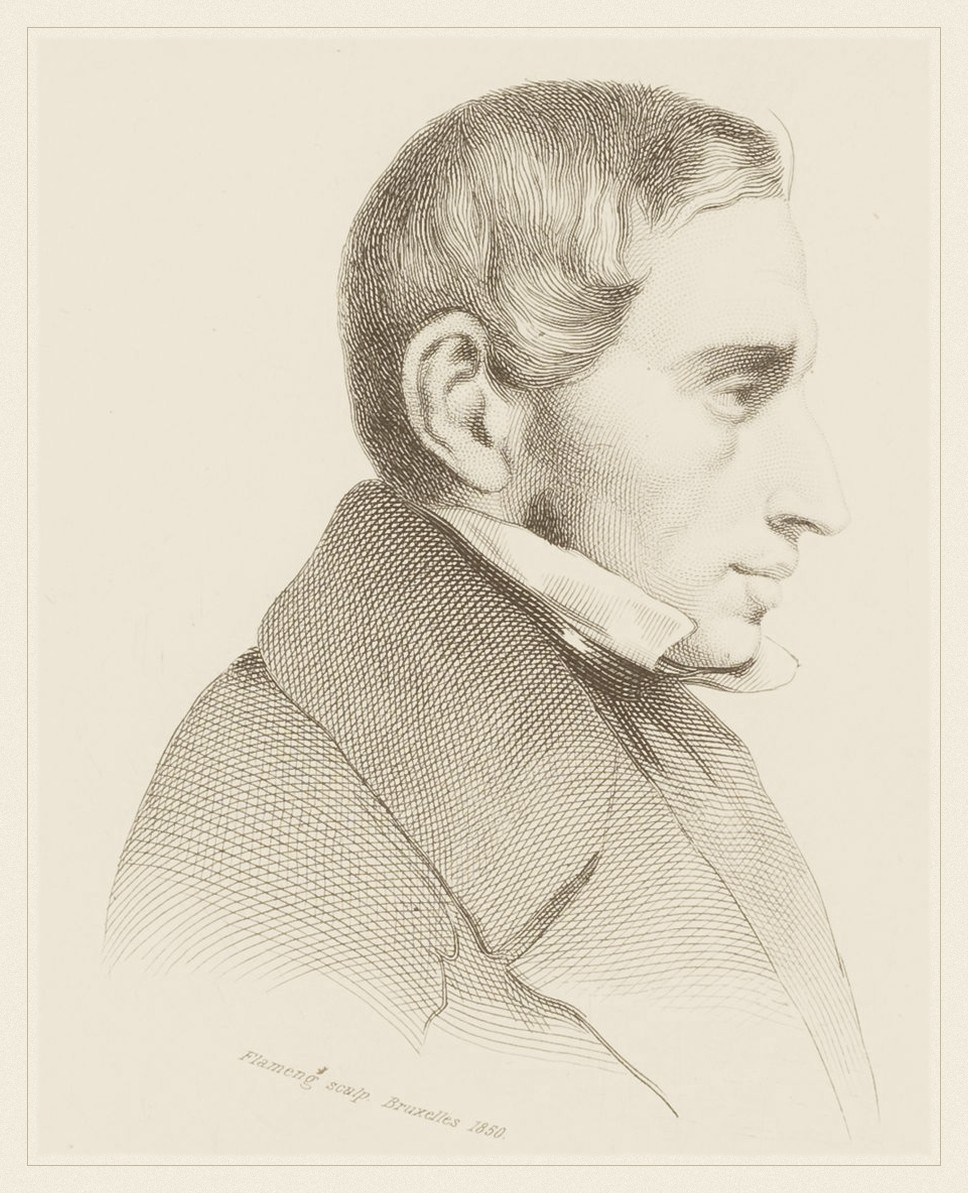
\includegraphics[keepaspectratio]{images/session-04-verhulst.jpg}}

\textbf{Pierre François Verhulst} · \textbf{1804--1849}

Named the logistic curve in 1845, modelling how populations stop
growing.

{Flameng, Léopold, 1850. Public domain, via Wikimedia Commons.}

\end{qmibplate}

\begin{qmibarchive}

\textbf{From the archive · Verhulst, 1845}

Malthus had argued that population grows geometrically while subsistence
grows arithmetically, so that catastrophe is arithmetic. Pierre François
Verhulst, a Belgian mathematician, thought the premise wrong: unchecked
exponential growth describes no actual population, because growth slows
as a population approaches what its territory can support.

He wrote down the correction. If growth is proportional both to the
current population and to the \emph{remaining room}, the result is a
curve that rises exponentially, inflects, and flattens toward a ceiling.
He named it the \emph{logistic} curve in 1845.

It arrived in statistics by a different road. Berkson proposed it in the
1940s as the natural transformation for dose-response data --- the
\emph{logit} --- arguing against the then-dominant probit on grounds of
tractability and interpretation (\citeproc{ref-berkson1944}{Berkson
1944}). Cox gave the regression treatment its modern form
(\citeproc{ref-cox1958}{Cox 1958}). The function Verhulst wrote to
describe populations pressing against a limit is now the standard way to
model any bounded probability, which is the same mathematical situation:
something that cannot exceed a ceiling and slows as it approaches one.

\begin{Shaded}
\begin{Highlighting}[]
\NormalTok{z }\OperatorTok{=}\NormalTok{ np.linspace(}\OperatorTok{{-}}\DecValTok{6}\NormalTok{, }\DecValTok{6}\NormalTok{, }\DecValTok{400}\NormalTok{)}
\NormalTok{sigma }\OperatorTok{=} \DecValTok{1} \OperatorTok{/}\NormalTok{ (}\DecValTok{1} \OperatorTok{+}\NormalTok{ np.exp(}\OperatorTok{{-}}\NormalTok{z))}

\NormalTok{fig, (ax1, ax2) }\OperatorTok{=}\NormalTok{ plt.subplots(}\DecValTok{1}\NormalTok{, }\DecValTok{2}\NormalTok{, figsize}\OperatorTok{=}\NormalTok{(}\FloatTok{9.4}\NormalTok{, }\FloatTok{3.9}\NormalTok{))}

\NormalTok{K }\OperatorTok{=} \DecValTok{100}
\NormalTok{ax1.plot(z, K }\OperatorTok{*}\NormalTok{ sigma, lw}\OperatorTok{=}\DecValTok{2}\NormalTok{, color}\OperatorTok{=}\NormalTok{CL.accent)}
\NormalTok{ax1.axhline(K, ls}\OperatorTok{=}\StringTok{"{-}{-}"}\NormalTok{, lw}\OperatorTok{=}\FloatTok{1.2}\NormalTok{, color}\OperatorTok{=}\NormalTok{CL.muted)}
\NormalTok{ax1.text(}\OperatorTok{{-}}\FloatTok{5.6}\NormalTok{, K }\OperatorTok{*} \FloatTok{1.03}\NormalTok{, }\StringTok{"carrying capacity $K$"}\NormalTok{, fontsize}\OperatorTok{=}\FloatTok{8.5}\NormalTok{, color}\OperatorTok{=}\NormalTok{CL.muted)}
\NormalTok{ax1.set\_xlabel(}\StringTok{"time"}\NormalTok{)}\OperatorTok{;}\NormalTok{ ax1.set\_ylabel(}\StringTok{"population"}\NormalTok{)}
\NormalTok{ax1.set\_title(}\StringTok{"Verhulst, 1845"}\NormalTok{, fontsize}\OperatorTok{=}\DecValTok{10}\NormalTok{, loc}\OperatorTok{=}\StringTok{"left"}\NormalTok{)}

\NormalTok{ax2.plot(z, sigma, lw}\OperatorTok{=}\DecValTok{2}\NormalTok{, color}\OperatorTok{=}\NormalTok{CL.accent)}
\ControlFlowTok{for}\NormalTok{ lev }\KeywordTok{in}\NormalTok{ (}\DecValTok{0}\NormalTok{, }\DecValTok{1}\NormalTok{):}
\NormalTok{    ax2.axhline(lev, ls}\OperatorTok{=}\StringTok{"{-}{-}"}\NormalTok{, lw}\OperatorTok{=}\FloatTok{1.2}\NormalTok{, color}\OperatorTok{=}\NormalTok{CL.muted)}
\NormalTok{ax2.plot([}\DecValTok{0}\NormalTok{], [}\FloatTok{0.5}\NormalTok{], marker}\OperatorTok{=}\StringTok{"o"}\NormalTok{, ms}\OperatorTok{=}\DecValTok{7}\NormalTok{, mfc}\OperatorTok{=}\StringTok{"none"}\NormalTok{, mec}\OperatorTok{=}\NormalTok{CL.warn, mew}\OperatorTok{=}\FloatTok{1.8}\NormalTok{)}
\NormalTok{ax2.annotate(}\StringTok{"steepest at $p=0.5$"}\NormalTok{, (}\DecValTok{0}\NormalTok{, }\FloatTok{0.5}\NormalTok{), textcoords}\OperatorTok{=}\StringTok{"offset points"}\NormalTok{,}
\NormalTok{             xytext}\OperatorTok{=}\NormalTok{(}\DecValTok{12}\NormalTok{, }\OperatorTok{{-}}\DecValTok{6}\NormalTok{), fontsize}\OperatorTok{=}\FloatTok{8.5}\NormalTok{, color}\OperatorTok{=}\NormalTok{CL.warn)}
\NormalTok{ax2.set\_xlabel(}\VerbatimStringTok{r"linear index }\DecValTok{$}\VerbatimStringTok{x}\DecValTok{\^{}}\CharTok{\textbackslash{}t}\VerbatimStringTok{op}\DecValTok{\textbackslash{}b}\VerbatimStringTok{eta}\DecValTok{$}\VerbatimStringTok{"}\NormalTok{)}\OperatorTok{;}\NormalTok{ ax2.set\_ylabel(}\VerbatimStringTok{r"}\DecValTok{$}\ErrorTok{\textbackslash{}}\VerbatimStringTok{Pr}\KeywordTok{(}\VerbatimStringTok{y=1}\KeywordTok{)}\DecValTok{$}\VerbatimStringTok{"}\NormalTok{)}
\NormalTok{ax2.set\_title(}\StringTok{"the same curve, as a probability"}\NormalTok{, fontsize}\OperatorTok{=}\DecValTok{10}\NormalTok{, loc}\OperatorTok{=}\StringTok{"left"}\NormalTok{)}

\NormalTok{fig.tight\_layout()}
\end{Highlighting}
\end{Shaded}

\begin{figure}[htbp]

\centering{

\pandocbounded{
\includegraphics[keepaspectratio]{session-04_files/figure-pdf/fig-logistic-output-1.png}}

}

\caption{\label{fig-logistic}The logistic function. Left: as Verhulst
wrote it, population against time approaching a carrying capacity.
Right: as statistics uses it, a probability against a linear index ---
the same curve, relabelled.}

\end{figure}%

\end{qmibarchive}

The model replaces the straight line with that curve. Write the linear
index as \(\eta_i = x_i^\top \beta\) and set

\[
\Pr(y_i = 1 \mid x_i) \;=\; \sigma(\eta_i) \;=\; \frac{1}{1 + e^{-\eta_i}}
\;=\; \frac{e^{\eta_i}}{1 + e^{\eta_i}} .
\]

The function is bounded strictly between 0 and 1, so the first failure
is gone by construction. It is symmetric about \(\eta = 0\), where
\(p = 0.5\) and the slope is steepest, and it flattens in both tails, so
the third failure is gone too: the same change in \(\eta\) moves the
probability a great deal in the middle and hardly at all at the
extremes.

Inverting it gives the form that explains the model's vocabulary:

\[
\log \underbrace{\frac{p_i}{1 - p_i}}_{\text{odds}} \;=\; x_i^\top \beta .
\]

The model is linear --- in the log-odds. That is the whole trick, and it
is why coefficients are not probabilities.

\section{Estimation: no formula, and why that is
fine}\label{estimation-no-formula-and-why-that-is-fine}

Least squares had a closed form. This does not. The log-likelihood is

\[
\ell(\beta) \;=\; \sum_i \Big[\, y_i \log \sigma(\eta_i) + (1 - y_i)\log\big(1 - \sigma(\eta_i)\big) \Big],
\]

and setting its derivative to zero gives
\(X^\top(y - \sigma(X\beta)) = 0\), which has no algebraic solution
because \(\sigma\) is nonlinear in \(\beta\). The estimate is found
numerically, by Newton--Raphson --- equivalently, by iteratively
reweighted least squares, which is the same computation dressed as a
sequence of weighted regressions.

This is less alarming than it sounds. The log-likelihood for logistic
regression is globally concave, so there is one maximum and any sensible
optimiser finds it. The exception matters and is covered below.

\phantomsection\label{check-loglik}
\begin{Shaded}
\begin{Highlighting}[]
\NormalTok{logit }\OperatorTok{=}\NormalTok{ sm.Logit(y, X).fit(disp}\OperatorTok{=}\DecValTok{0}\NormalTok{)}
\NormalTok{eta }\OperatorTok{=}\NormalTok{ X.to\_numpy() }\OperatorTok{@}\NormalTok{ logit.params.to\_numpy()}
\NormalTok{p }\OperatorTok{=} \DecValTok{1} \OperatorTok{/}\NormalTok{ (}\DecValTok{1} \OperatorTok{+}\NormalTok{ np.exp(}\OperatorTok{{-}}\NormalTok{eta))}

\CommentTok{\# The likelihood, written straight from the definition.}
\NormalTok{ll\_hand }\OperatorTok{=}\NormalTok{ (y }\OperatorTok{*}\NormalTok{ np.log(p) }\OperatorTok{+}\NormalTok{ (}\DecValTok{1} \OperatorTok{{-}}\NormalTok{ y) }\OperatorTok{*}\NormalTok{ np.log(}\DecValTok{1} \OperatorTok{{-}}\NormalTok{ p)).}\BuiltInTok{sum}\NormalTok{()}
\BuiltInTok{print}\NormalTok{(}\SpecialStringTok{f"log{-}likelihood by hand  }\SpecialCharTok{\{}\NormalTok{ll\_hand}\SpecialCharTok{:\textgreater{}12.6f\}}\SpecialStringTok{"}\NormalTok{)}
\BuiltInTok{print}\NormalTok{(}\SpecialStringTok{f"statsmodels             }\SpecialCharTok{\{}\NormalTok{logit}\SpecialCharTok{.}\NormalTok{llf}\SpecialCharTok{:\textgreater{}12.6f\}}\SpecialStringTok{"}\NormalTok{)}

\CommentTok{\# At the optimum the score must vanish: X\textquotesingle{}(y {-} p) = 0.}
\NormalTok{score }\OperatorTok{=}\NormalTok{ X.to\_numpy().T }\OperatorTok{@}\NormalTok{ (y.to\_numpy() }\OperatorTok{{-}}\NormalTok{ p)}
\BuiltInTok{print}\NormalTok{(}\SpecialStringTok{f"}\CharTok{\textbackslash{}n}\SpecialStringTok{score X\textquotesingle{}(y {-} p) at the optimum, largest element: }\SpecialCharTok{\{}\NormalTok{np}\SpecialCharTok{.}\BuiltInTok{abs}\NormalTok{(score)}\SpecialCharTok{.}\BuiltInTok{max}\NormalTok{()}\SpecialCharTok{:.2e\}}\SpecialStringTok{"}\NormalTok{)}
\BuiltInTok{print}\NormalTok{(}\StringTok{"  (zero to numerical tolerance — that is what \textquotesingle{}converged\textquotesingle{} means)"}\NormalTok{)}

\BuiltInTok{print}\NormalTok{(}\SpecialStringTok{f"}\CharTok{\textbackslash{}n}\SpecialStringTok{null log{-}likelihood     }\SpecialCharTok{\{}\NormalTok{logit}\SpecialCharTok{.}\NormalTok{llnull}\SpecialCharTok{:\textgreater{}12.4f\}}\SpecialStringTok{"}\NormalTok{)}
\BuiltInTok{print}\NormalTok{(}\SpecialStringTok{f"McFadden pseudo{-}R²      }\SpecialCharTok{\{}\DecValTok{1} \OperatorTok{{-}}\NormalTok{ logit}\SpecialCharTok{.}\NormalTok{llf}\OperatorTok{/}\NormalTok{logit}\SpecialCharTok{.}\NormalTok{llnull}\SpecialCharTok{:\textgreater{}12.5f\}}\SpecialStringTok{"}\NormalTok{)}
\end{Highlighting}
\end{Shaded}

\begin{verbatim}
log-likelihood by hand  -4068.055780
statsmodels             -4068.055780

score X'(y - p) at the optimum, largest element: 5.09e-11
  (zero to numerical tolerance — that is what 'converged' means)

null log-likelihood       -4212.0203
McFadden pseudo-R²           0.03418
\end{verbatim}

The pseudo-\(R^2\) is 0.034, and that number deserves a warning.
McFadden's statistic is \emph{not} a proportion of variance explained
and does not behave like \(R^2\); values that would be alarming in a
linear model are ordinary here. Comparing it across models fitted to
different samples, or treating 0.034 as ``3.4\% of something'', is a
misreading.

\section{Reading the coefficients}\label{reading-the-coefficients}

A logistic coefficient is a change in log-odds per unit of the
predictor. Nobody thinks in log-odds. There are three standard
translations, in increasing order of usefulness and decreasing order of
popularity.

\begin{qmibdefinition}

{\textbf{Odds ratio}} --- \(e^{\beta_j}\), the multiplicative change in
the odds per one-unit increase in \(x_j\), holding the rest of the index
fixed. Constant across the range of \(x\), which is its convenience and
its trap: constant on the odds scale means \emph{not} constant on the
probability scale.

\end{qmibdefinition}

\begin{qmibdefinition}

{\textbf{Marginal effect}} ---
\(\partial p / \partial x_j = \beta_j\, p(1-p)\), the change in
probability per unit of \(x_j\). It depends on where you are: the same
coefficient moves the probability most near \(p = 0.5\) and least in the
tails. The \emph{average marginal effect} averages it over the observed
sample, which is usually the number a reader wants.

\end{qmibdefinition}

\begin{qmibdefinition}

{\textbf{Predicted probability}} --- \(\sigma(x^\top\hat\beta)\)
evaluated at specified values. The most honest presentation for a
non-technical audience, because it makes the nonlinearity visible
instead of hiding it in a ratio.

\end{qmibdefinition}

\phantomsection\label{check-effects}
\begin{Shaded}
\begin{Highlighting}[]
\NormalTok{b\_fico }\OperatorTok{=}\NormalTok{ logit.params[}\StringTok{"fico"}\NormalTok{]}
\BuiltInTok{print}\NormalTok{(}\SpecialStringTok{f"coefficient on fico         }\SpecialCharTok{\{}\NormalTok{b\_fico}\SpecialCharTok{:+.6f\}}\SpecialStringTok{  (log{-}odds per point)"}\NormalTok{)}
\BuiltInTok{print}\NormalTok{(}\SpecialStringTok{f"odds ratio, per point       }\SpecialCharTok{\{}\NormalTok{np}\SpecialCharTok{.}\NormalTok{exp(b\_fico)}\SpecialCharTok{:.5f\}}\SpecialStringTok{"}\NormalTok{)}
\BuiltInTok{print}\NormalTok{(}\SpecialStringTok{f"odds ratio, per 10 points   }\SpecialCharTok{\{}\NormalTok{np}\SpecialCharTok{.}\NormalTok{exp(}\DecValTok{10} \OperatorTok{*}\NormalTok{ b\_fico)}\SpecialCharTok{:.4f\}}\SpecialStringTok{"}\NormalTok{)}

\NormalTok{ame }\OperatorTok{=}\NormalTok{ (b\_fico }\OperatorTok{*}\NormalTok{ p }\OperatorTok{*}\NormalTok{ (}\DecValTok{1} \OperatorTok{{-}}\NormalTok{ p)).mean()}
\BuiltInTok{print}\NormalTok{(}\SpecialStringTok{f"}\CharTok{\textbackslash{}n}\SpecialStringTok{average marginal effect     }\SpecialCharTok{\{}\NormalTok{ame}\SpecialCharTok{:+.8f\}}\SpecialStringTok{ per point"}\NormalTok{)}
\BuiltInTok{print}\NormalTok{(}\SpecialStringTok{f"  = }\SpecialCharTok{\{}\NormalTok{ame }\OperatorTok{*} \DecValTok{10} \OperatorTok{*} \DecValTok{100}\SpecialCharTok{:+.3f\}}\SpecialStringTok{ percentage points per 10 FICO points"}\NormalTok{)}
\BuiltInTok{print}\NormalTok{(}\SpecialStringTok{f"  statsmodels margeff:      }\SpecialCharTok{\{}\NormalTok{logit}\SpecialCharTok{.}\NormalTok{get\_margeff()}\SpecialCharTok{.}\NormalTok{margeff[}\DecValTok{0}\NormalTok{]}\SpecialCharTok{:+.8f\}}\SpecialStringTok{"}\NormalTok{)}

\CommentTok{\# The same coefficient, at three different places on the curve.}
\BuiltInTok{print}\NormalTok{(}\StringTok{"}\CharTok{\textbackslash{}n}\StringTok{the marginal effect is not one number:"}\NormalTok{)}
\ControlFlowTok{for}\NormalTok{ label, pv }\KeywordTok{in}\NormalTok{ ((}\StringTok{"a safe borrower  (p=0.05)"}\NormalTok{, }\FloatTok{0.05}\NormalTok{),}
\NormalTok{                  (}\StringTok{"a typical one    (p=0.16)"}\NormalTok{, y.mean()),}
\NormalTok{                  (}\StringTok{"a risky one      (p=0.50)"}\NormalTok{, }\FloatTok{0.50}\NormalTok{)):}
    \BuiltInTok{print}\NormalTok{(}\SpecialStringTok{f"  }\SpecialCharTok{\{}\NormalTok{label}\SpecialCharTok{\}}\SpecialStringTok{: }\SpecialCharTok{\{}\NormalTok{b\_fico }\OperatorTok{*}\NormalTok{ pv }\OperatorTok{*}\NormalTok{ (}\DecValTok{1}\OperatorTok{{-}}\NormalTok{pv) }\OperatorTok{*} \DecValTok{10} \OperatorTok{*} \DecValTok{100}\SpecialCharTok{:+.3f\}}\SpecialStringTok{ pp per 10 points"}\NormalTok{)}
\end{Highlighting}
\end{Shaded}

\begin{verbatim}
coefficient on fico         -0.005655  (log-odds per point)
odds ratio, per point       0.99436
odds ratio, per 10 points   0.9450

average marginal effect     -0.00073738 per point
  = -0.737 percentage points per 10 FICO points
  statsmodels margeff:      -0.00073738

the marginal effect is not one number:
  a safe borrower  (p=0.05): -0.269 pp per 10 points
  a typical one    (p=0.16): -0.760 pp per 10 points
  a risky one      (p=0.50): -1.414 pp per 10 points
\end{verbatim}

The last block is the argument against reporting odds ratios alone. One
coefficient, one odds ratio --- and a change of 10 FICO points moves the
probability three times as much for a borderline borrower as for a safe
one. An odds ratio conceals that; a marginal effect or a plot of
predicted probabilities shows it.

There is a subtler problem with odds ratios that is widely committed.
Logistic coefficients are identified only up to the scale of the
unobserved error, and that scale changes when predictors are added ---
so coefficients from nested logistic models are \textbf{not comparable}
the way linear coefficients are, and an apparent change on adding a
control may be pure rescaling (\citeproc{ref-mood2009}{Mood 2009}).
Compare average marginal effects or predicted probabilities across
specifications, not raw coefficients or odds ratios.

\section{Comparing models: the likelihood-ratio
test}\label{comparing-models-the-likelihood-ratio-test}

With no sums of squares there is no \(F\) test, but the likelihood
supplies the analogue. For nested models, twice the difference in
log-likelihood is asymptotically \(\chi^2\) with degrees of freedom
equal to the number of restrictions:

\[
\mathrm{LR} \;=\; 2\big(\ell_{\text{full}} - \ell_{\text{restricted}}\big)
\;\overset{d}{\longrightarrow}\; \chi^2_q .
\]

\phantomsection\label{check-lr}
\begin{Shaded}
\begin{Highlighting}[]
\ImportTok{from}\NormalTok{ scipy }\ImportTok{import}\NormalTok{ stats }\ImportTok{as}\NormalTok{ st}

\NormalTok{full }\OperatorTok{=}\NormalTok{ logit}
\NormalTok{small }\OperatorTok{=}\NormalTok{ sm.Logit(y, sm.add\_constant(loans[[}\StringTok{"fico"}\NormalTok{, }\StringTok{"int\_rate"}\NormalTok{, }\StringTok{"log\_annual\_inc"}\NormalTok{]])).fit(disp}\OperatorTok{=}\DecValTok{0}\NormalTok{)}

\NormalTok{lr }\OperatorTok{=} \DecValTok{2} \OperatorTok{*}\NormalTok{ (full.llf }\OperatorTok{{-}}\NormalTok{ small.llf)}
\NormalTok{pval }\OperatorTok{=}\NormalTok{ st.chi2.sf(lr, df}\OperatorTok{=}\DecValTok{1}\NormalTok{)}
\BuiltInTok{print}\NormalTok{(}\SpecialStringTok{f"full model      log{-}likelihood }\SpecialCharTok{\{}\NormalTok{full}\SpecialCharTok{.}\NormalTok{llf}\SpecialCharTok{:12.4f\}}\SpecialStringTok{"}\NormalTok{)}
\BuiltInTok{print}\NormalTok{(}\SpecialStringTok{f"without dti     log{-}likelihood }\SpecialCharTok{\{}\NormalTok{small}\SpecialCharTok{.}\NormalTok{llf}\SpecialCharTok{:12.4f\}}\SpecialStringTok{"}\NormalTok{)}
\BuiltInTok{print}\NormalTok{(}\SpecialStringTok{f"}\CharTok{\textbackslash{}n}\SpecialStringTok{LR statistic }\SpecialCharTok{\{}\NormalTok{lr}\SpecialCharTok{:.4f\}}\SpecialStringTok{ on 1 df,  p = }\SpecialCharTok{\{}\NormalTok{pval}\SpecialCharTok{:.4f\}}\SpecialStringTok{"}\NormalTok{)}
\BuiltInTok{print}\NormalTok{(}\StringTok{"dti adds nothing detectable here."} \ControlFlowTok{if}\NormalTok{ pval }\OperatorTok{\textgreater{}} \FloatTok{0.05} \ControlFlowTok{else} \StringTok{"dti matters."}\NormalTok{)}
\end{Highlighting}
\end{Shaded}

\begin{verbatim}
full model      log-likelihood   -4068.0558
without dti     log-likelihood   -4068.0850

LR statistic 0.0584 on 1 df,  p = 0.8090
dti adds nothing detectable here.
\end{verbatim}

Note the discipline this enforces. Both models must be fitted to
\emph{the same rows} --- a predictor with extra missing values silently
changes the sample and the comparison becomes meaningless --- and the
test only applies to nested models. For non-nested candidates, AIC from
chapter 3 is the tool.

\section{Does the model discriminate, and is it
calibrated?}\label{does-the-model-discriminate-and-is-it-calibrated}

Two different questions, routinely conflated.

\begin{qmibdefinition}

{\textbf{Discrimination}} --- can the model rank? The area under the ROC
curve is exactly the probability that a randomly chosen positive case
receives a higher predicted probability than a randomly chosen negative
one (\citeproc{ref-hanley1982}{Hanley and McNeil 1982}). 0.5 is
coin-flipping; 1.0 is perfect separation.

\end{qmibdefinition}

\begin{qmibdefinition}

{\textbf{Calibration}} --- are the probabilities \emph{true}? Among
cases assigned 0.30, do about 30\% turn out positive? The Brier score,
the mean squared difference between predicted probability and outcome,
penalises both errors at once (\citeproc{ref-brier1950}{Brier 1950}).

\end{qmibdefinition}

A model can discriminate well and be badly calibrated, or the reverse.
Which matters depends entirely on the use: a ranking for a limited
budget of inspections needs discrimination; a price that must reflect
risk needs calibration.

\phantomsection\label{check-auc}
\begin{Shaded}
\begin{Highlighting}[]
\ImportTok{from}\NormalTok{ scipy.stats }\ImportTok{import}\NormalTok{ rankdata}
\ImportTok{from}\NormalTok{ sklearn.metrics }\ImportTok{import}\NormalTok{ roc\_auc\_score, brier\_score\_loss}

\CommentTok{\# AUC = P(score of a random positive \textgreater{} score of a random negative). That is the}
\CommentTok{\# Mann{-}Whitney U statistic, so it can be computed from ranks alone.}
\NormalTok{r }\OperatorTok{=}\NormalTok{ rankdata(p)}
\NormalTok{n1, n0 }\OperatorTok{=} \BuiltInTok{int}\NormalTok{(y.}\BuiltInTok{sum}\NormalTok{()), }\BuiltInTok{int}\NormalTok{(}\BuiltInTok{len}\NormalTok{(y) }\OperatorTok{{-}}\NormalTok{ y.}\BuiltInTok{sum}\NormalTok{())}
\NormalTok{auc\_hand }\OperatorTok{=}\NormalTok{ (r[y }\OperatorTok{==} \DecValTok{1}\NormalTok{].}\BuiltInTok{sum}\NormalTok{() }\OperatorTok{{-}}\NormalTok{ n1 }\OperatorTok{*}\NormalTok{ (n1 }\OperatorTok{+} \DecValTok{1}\NormalTok{) }\OperatorTok{/} \DecValTok{2}\NormalTok{) }\OperatorTok{/}\NormalTok{ (n1 }\OperatorTok{*}\NormalTok{ n0)}

\BuiltInTok{print}\NormalTok{(}\SpecialStringTok{f"AUC by hand (Mann{-}Whitney)  }\SpecialCharTok{\{}\NormalTok{auc\_hand}\SpecialCharTok{:.6f\}}\SpecialStringTok{"}\NormalTok{)}
\BuiltInTok{print}\NormalTok{(}\SpecialStringTok{f"sklearn roc\_auc\_score       }\SpecialCharTok{\{}\NormalTok{roc\_auc\_score(y, p)}\SpecialCharTok{:.6f\}}\SpecialStringTok{"}\NormalTok{)}

\NormalTok{brier }\OperatorTok{=}\NormalTok{ brier\_score\_loss(y, p)}
\NormalTok{base }\OperatorTok{=}\NormalTok{ np.mean((y }\OperatorTok{{-}}\NormalTok{ y.mean()) }\OperatorTok{**} \DecValTok{2}\NormalTok{)}
\BuiltInTok{print}\NormalTok{(}\SpecialStringTok{f"}\CharTok{\textbackslash{}n}\SpecialStringTok{Brier score            }\SpecialCharTok{\{}\NormalTok{brier}\SpecialCharTok{:.6f\}}\SpecialStringTok{"}\NormalTok{)}
\BuiltInTok{print}\NormalTok{(}\SpecialStringTok{f"predicting the base rate }\SpecialCharTok{\{}\NormalTok{base}\SpecialCharTok{:.6f\}}\SpecialStringTok{"}\NormalTok{)}
\BuiltInTok{print}\NormalTok{(}\SpecialStringTok{f"skill over base rate:  }\SpecialCharTok{\{}\DecValTok{1} \OperatorTok{{-}}\NormalTok{ brier}\OperatorTok{/}\NormalTok{base}\SpecialCharTok{:.2\%\}}\SpecialStringTok{"}\NormalTok{)}
\end{Highlighting}
\end{Shaded}

\begin{verbatim}
AUC by hand (Mann-Whitney)  0.629502
sklearn roc_auc_score       0.629502

Brier score            0.130664
predicting the base rate 0.134437
skill over base rate:  2.81%
\end{verbatim}

Both numbers are sobering and should be reported that way. An AUC of
0.63 is weak discrimination --- better than chance, far from useful for
an individual decision. The Brier score improves on simply predicting
the base rate for everyone by under 3\%. The model is real, in the sense
that its coefficients are estimated precisely and the likelihood-ratio
tests are significant, and it is close to useless as a device for
deciding about a particular borrower. Those two facts are compatible,
and a large \(n\) is what makes them compatible: with 9,578
observations, a very weak signal is statistically unmistakable.

\section{When the outcome is ordered}\label{when-the-outcome-is-ordered}

Some categorical outcomes have an order --- unlikely, somewhat likely,
very likely. Multinomial logit would ignore the ordering; separate
binary models would waste it. The ordinal model uses it, by fitting one
slope and several thresholds:

\[
\Pr(y_i \le j) \;=\; \sigma(\tau_j - x_i^\top\beta),
\qquad \tau_1 < \tau_2 < \dots < \tau_{J-1} .
\]

Each threshold \(\tau_j\) marks a cut on the latent scale; the
\emph{same} \(\beta\) shifts every cut together. That is the
proportional-odds assumption, and it is a real restriction: the effect
of a predictor on moving from ``unlikely'' to ``somewhat likely'' is
assumed identical to its effect on moving from ``somewhat likely'' to
``very likely''.

\phantomsection\label{check-ordinal}
\begin{Shaded}
\begin{Highlighting}[]
\ImportTok{from}\NormalTok{ statsmodels.miscmodels.ordinal\_model }\ImportTok{import}\NormalTok{ OrderedModel}

\NormalTok{grad }\OperatorTok{=}\NormalTok{ qmib.load(}\StringTok{"ologit"}\NormalTok{)}
\NormalTok{grad[}\StringTok{"apply\_c"}\NormalTok{] }\OperatorTok{=}\NormalTok{ pd.Categorical(}
\NormalTok{    grad[}\StringTok{"apply"}\NormalTok{], categories}\OperatorTok{=}\NormalTok{[}\StringTok{"unlikely"}\NormalTok{, }\StringTok{"somewhat likely"}\NormalTok{, }\StringTok{"very likely"}\NormalTok{], ordered}\OperatorTok{=}\VariableTok{True}\NormalTok{)}

\NormalTok{om }\OperatorTok{=}\NormalTok{ OrderedModel(grad[}\StringTok{"apply\_c"}\NormalTok{], grad[[}\StringTok{"pared"}\NormalTok{, }\StringTok{"public"}\NormalTok{, }\StringTok{"gpa"}\NormalTok{]],}
\NormalTok{                  distr}\OperatorTok{=}\StringTok{"logit"}\NormalTok{).fit(method}\OperatorTok{=}\StringTok{"bfgs"}\NormalTok{, disp}\OperatorTok{=}\DecValTok{0}\NormalTok{)}

\BuiltInTok{print}\NormalTok{(}\SpecialStringTok{f"n = }\SpecialCharTok{\{}\BuiltInTok{len}\NormalTok{(grad)}\SpecialCharTok{\}}\SpecialStringTok{   outcome: }\SpecialCharTok{\{}\BuiltInTok{list}\NormalTok{(grad[}\StringTok{\textquotesingle{}apply\_c\textquotesingle{}}\NormalTok{].cat.categories)}\SpecialCharTok{\}}\SpecialStringTok{"}\NormalTok{)}
\BuiltInTok{print}\NormalTok{(}\SpecialStringTok{f"}\CharTok{\textbackslash{}n}\SpecialCharTok{\{}\StringTok{\textquotesingle{}predictor\textquotesingle{}}\SpecialCharTok{:12\}\{}\StringTok{\textquotesingle{}coef\textquotesingle{}}\SpecialCharTok{:\textgreater{}10\}\{}\StringTok{\textquotesingle{}odds ratio\textquotesingle{}}\SpecialCharTok{:\textgreater{}13\}}\SpecialStringTok{"}\NormalTok{)}
\ControlFlowTok{for}\NormalTok{ name }\KeywordTok{in}\NormalTok{ [}\StringTok{"pared"}\NormalTok{, }\StringTok{"public"}\NormalTok{, }\StringTok{"gpa"}\NormalTok{]:}
\NormalTok{    b }\OperatorTok{=}\NormalTok{ om.params[name]}
    \BuiltInTok{print}\NormalTok{(}\SpecialStringTok{f"}\SpecialCharTok{\{}\NormalTok{name}\SpecialCharTok{:12\}\{}\NormalTok{b}\SpecialCharTok{:10.4f\}\{}\NormalTok{np}\SpecialCharTok{.}\NormalTok{exp(b)}\SpecialCharTok{:13.4f\}}\SpecialStringTok{"}\NormalTok{)}
\BuiltInTok{print}\NormalTok{(}\SpecialStringTok{f"}\CharTok{\textbackslash{}n}\SpecialStringTok{thresholds (latent cutpoints): "}
      \SpecialStringTok{f"}\SpecialCharTok{\{}\StringTok{\textquotesingle{}, \textquotesingle{}}\SpecialCharTok{.}\NormalTok{join(}\SpecialStringTok{f\textquotesingle{}}\SpecialCharTok{\{}\NormalTok{v}\SpecialCharTok{:.3f\}}\SpecialStringTok{\textquotesingle{}} \ControlFlowTok{for}\NormalTok{ v }\KeywordTok{in}\NormalTok{ om.params[}\OperatorTok{{-}}\DecValTok{2}\NormalTok{:].values)}\SpecialCharTok{\}}\SpecialStringTok{"}\NormalTok{)}
\BuiltInTok{print}\NormalTok{(}\StringTok{"}\CharTok{\textbackslash{}n}\StringTok{One slope per predictor, two cutpoints — that is the proportional{-}odds"}\NormalTok{)}
\BuiltInTok{print}\NormalTok{(}\StringTok{"restriction. Test it before relying on it (Brant 1990); if it fails, a"}\NormalTok{)}
\BuiltInTok{print}\NormalTok{(}\StringTok{"multinomial model that ignores the ordering is the honest fallback."}\NormalTok{)}
\end{Highlighting}
\end{Shaded}

\begin{verbatim}
n = 400   outcome: ['unlikely', 'somewhat likely', 'very likely']

predictor         coef   odds ratio
pared           1.0476       2.8509
public         -0.0586       0.9431
gpa             0.6158       1.8512

thresholds (latent cutpoints): 2.204, 0.740

One slope per predictor, two cutpoints — that is the proportional-odds
restriction. Test it before relying on it (Brant 1990); if it fails, a
multinomial model that ignores the ordering is the honest fallback.
\end{verbatim}

Having a parent with a graduate degree multiplies the odds of being in a
higher application category by about 2.85. The assumption that this
multiplier is the same at both cutpoints should be tested rather than
assumed (\citeproc{ref-brant1990}{Brant 1990}); when it fails, either a
partial-proportional-odds model or the unordered multinomial below is
preferable to a restriction the data reject.

\section{When the categories have no
order}\label{when-the-categories-have-no-order}

With \(J\) unordered categories, one is chosen as the baseline and
\(J-1\) binary comparisons are estimated jointly:

\[
\log \frac{\Pr(y_i = j)}{\Pr(y_i = \text{baseline})} \;=\; x_i^\top\beta_j ,
\qquad j \ne \text{baseline}.
\]

Every coefficient is therefore relative to the baseline, and changing
the baseline changes all of them --- without changing a single fitted
probability. A multinomial result reported without naming the baseline
cannot be read.

\phantomsection\label{check-multinomial}
\begin{Shaded}
\begin{Highlighting}[]
\NormalTok{hs }\OperatorTok{=}\NormalTok{ qmib.load(}\StringTok{"hsbdemo"}\NormalTok{)}
\NormalTok{hs[}\StringTok{"prog\_c"}\NormalTok{] }\OperatorTok{=}\NormalTok{ pd.Categorical(hs[}\StringTok{"prog"}\NormalTok{], categories}\OperatorTok{=}\NormalTok{[}\StringTok{"academic"}\NormalTok{, }\StringTok{"general"}\NormalTok{, }\StringTok{"vocation"}\NormalTok{])}
\NormalTok{ses\_code }\OperatorTok{=}\NormalTok{ pd.Categorical(hs[}\StringTok{"ses"}\NormalTok{], categories}\OperatorTok{=}\NormalTok{[}\StringTok{"low"}\NormalTok{, }\StringTok{"middle"}\NormalTok{, }\StringTok{"high"}\NormalTok{]).codes}

\NormalTok{mn }\OperatorTok{=}\NormalTok{ sm.MNLogit(hs[}\StringTok{"prog\_c"}\NormalTok{].cat.codes,}
\NormalTok{                sm.add\_constant(hs[[}\StringTok{"write"}\NormalTok{]].assign(ses}\OperatorTok{=}\NormalTok{ses\_code))).fit(disp}\OperatorTok{=}\DecValTok{0}\NormalTok{)}

\BuiltInTok{print}\NormalTok{(}\SpecialStringTok{f"n = }\SpecialCharTok{\{}\BuiltInTok{len}\NormalTok{(hs)}\SpecialCharTok{\}}\SpecialStringTok{   baseline = academic"}\NormalTok{)}
\BuiltInTok{print}\NormalTok{(}\SpecialStringTok{f"}\CharTok{\textbackslash{}n}\SpecialCharTok{\{}\StringTok{\textquotesingle{}\textquotesingle{}}\SpecialCharTok{:10\}\{}\StringTok{\textquotesingle{}general\textquotesingle{}}\SpecialCharTok{:\textgreater{}12\}\{}\StringTok{\textquotesingle{}vocation\textquotesingle{}}\SpecialCharTok{:\textgreater{}12\}}\SpecialStringTok{"}\NormalTok{)}
\ControlFlowTok{for}\NormalTok{ i, name }\KeywordTok{in} \BuiltInTok{enumerate}\NormalTok{([}\StringTok{"const"}\NormalTok{, }\StringTok{"write"}\NormalTok{, }\StringTok{"ses"}\NormalTok{]):}
    \BuiltInTok{print}\NormalTok{(}\SpecialStringTok{f"}\SpecialCharTok{\{}\NormalTok{name}\SpecialCharTok{:10\}\{}\NormalTok{mn}\SpecialCharTok{.}\NormalTok{params}\SpecialCharTok{.}\NormalTok{iloc[i,}\DecValTok{0}\NormalTok{]}\SpecialCharTok{:12.4f\}\{}\NormalTok{mn}\SpecialCharTok{.}\NormalTok{params}\SpecialCharTok{.}\NormalTok{iloc[i,}\DecValTok{1}\NormalTok{]}\SpecialCharTok{:12.4f\}}\SpecialStringTok{"}\NormalTok{)}
\BuiltInTok{print}\NormalTok{(}\SpecialStringTok{f"}\CharTok{\textbackslash{}n}\SpecialStringTok{odds ratio for a 1{-}point writing score:"}\NormalTok{)}
\BuiltInTok{print}\NormalTok{(}\SpecialStringTok{f"  general  vs academic  }\SpecialCharTok{\{}\NormalTok{np}\SpecialCharTok{.}\NormalTok{exp(mn.params.iloc[}\DecValTok{1}\NormalTok{,}\DecValTok{0}\NormalTok{])}\SpecialCharTok{:.4f\}}\SpecialStringTok{"}\NormalTok{)}
\BuiltInTok{print}\NormalTok{(}\SpecialStringTok{f"  vocation vs academic  }\SpecialCharTok{\{}\NormalTok{np}\SpecialCharTok{.}\NormalTok{exp(mn.params.iloc[}\DecValTok{1}\NormalTok{,}\DecValTok{1}\NormalTok{])}\SpecialCharTok{:.4f\}}\SpecialStringTok{"}\NormalTok{)}
\BuiltInTok{print}\NormalTok{(}\SpecialStringTok{f"}\CharTok{\textbackslash{}n}\SpecialStringTok{McFadden pseudo{-}R² }\SpecialCharTok{\{}\DecValTok{1} \OperatorTok{{-}}\NormalTok{ mn}\SpecialCharTok{.}\NormalTok{llf}\OperatorTok{/}\NormalTok{mn}\SpecialCharTok{.}\NormalTok{llnull}\SpecialCharTok{:.4f\}}\SpecialStringTok{"}\NormalTok{)}
\end{Highlighting}
\end{Shaded}

\begin{verbatim}
n = 200   baseline = academic

               general    vocation
const           2.9426      5.5388
write          -0.0582     -0.1122
ses            -0.6367     -0.4512

odds ratio for a 1-point writing score:
  general  vs academic  0.9435
  vocation vs academic  0.8939

McFadden pseudo-R² 0.1072
\end{verbatim}

The multinomial model carries an assumption that the ordinal one does
not: \emph{independence of irrelevant alternatives}. The ratio of
probabilities for any two categories must not depend on what other
categories exist. When alternatives are close substitutes the assumption
fails, and the classic illustration is a transport choice between car,
red bus and blue bus --- introducing a bus of a different colour should
not change the car's share, and in a multinomial logit it does.

\section{The failure mode worth
knowing}\label{the-failure-mode-worth-knowing}

Logistic regression has one dramatic failure, and it looks like success.

\begin{qmibdefinition}

{\textbf{Separation}} --- a predictor, or a combination of them,
perfectly predicts the outcome in the sample. The likelihood then has no
maximum: pushing the coefficient toward infinity keeps improving the
fit, so the optimiser diverges. Estimates come back enormous with
enormous standard errors, or the software reports non-convergence
(\citeproc{ref-albert1984}{Albert and Anderson 1984}).

\end{qmibdefinition}

\phantomsection\label{check-separation}
\begin{Shaded}
\begin{Highlighting}[]
\NormalTok{rng }\OperatorTok{=}\NormalTok{ np.random.default\_rng(}\DecValTok{60033}\NormalTok{)}
\NormalTok{n }\OperatorTok{=} \DecValTok{60}
\NormalTok{x }\OperatorTok{=}\NormalTok{ rng.normal(size}\OperatorTok{=}\NormalTok{n)}
\NormalTok{yy }\OperatorTok{=}\NormalTok{ (x }\OperatorTok{\textgreater{}} \DecValTok{0}\NormalTok{).astype(}\BuiltInTok{int}\NormalTok{)          }\CommentTok{\# perfectly separated by construction}

\BuiltInTok{print}\NormalTok{(}\SpecialStringTok{f"n = }\SpecialCharTok{\{}\NormalTok{n}\SpecialCharTok{\}}\SpecialStringTok{;  the outcome is exactly 1 when x \textgreater{} 0, with no exceptions."}\NormalTok{)}

\ControlFlowTok{try}\NormalTok{:}
\NormalTok{    sep }\OperatorTok{=}\NormalTok{ sm.Logit(yy, sm.add\_constant(x)).fit(disp}\OperatorTok{=}\DecValTok{0}\NormalTok{, maxiter}\OperatorTok{=}\DecValTok{200}\NormalTok{)}
    \BuiltInTok{print}\NormalTok{(}\SpecialStringTok{f"}\CharTok{\textbackslash{}n}\SpecialStringTok{coefficient   }\SpecialCharTok{\{}\NormalTok{np}\SpecialCharTok{.}\NormalTok{asarray(sep.params)[}\DecValTok{1}\NormalTok{]}\SpecialCharTok{:\textgreater{}14,.2f\}}\SpecialStringTok{"}\NormalTok{)}
    \BuiltInTok{print}\NormalTok{(}\SpecialStringTok{f"std. error    }\SpecialCharTok{\{}\NormalTok{np}\SpecialCharTok{.}\NormalTok{asarray(sep.bse)[}\DecValTok{1}\NormalTok{]}\SpecialCharTok{:\textgreater{}14,.2f\}}\SpecialStringTok{"}\NormalTok{)}
    \BuiltInTok{print}\NormalTok{(}\SpecialStringTok{f"converged     }\SpecialCharTok{\{}\NormalTok{sep}\SpecialCharTok{.}\NormalTok{mle\_retvals[}\StringTok{\textquotesingle{}converged\textquotesingle{}}\NormalTok{]}\SpecialCharTok{\}}\SpecialStringTok{"}\NormalTok{)}
\ControlFlowTok{except} \PreprocessorTok{Exception} \ImportTok{as}\NormalTok{ exc:}
    \BuiltInTok{print}\NormalTok{(}\SpecialStringTok{f"}\CharTok{\textbackslash{}n}\SpecialStringTok{estimation failed: }\SpecialCharTok{\{}\BuiltInTok{type}\NormalTok{(exc)}\SpecialCharTok{.}\VariableTok{\_\_name\_\_}\SpecialCharTok{\}}\SpecialStringTok{: }\SpecialCharTok{\{}\NormalTok{exc}\SpecialCharTok{\}}\SpecialStringTok{"}\NormalTok{)}

\BuiltInTok{print}\NormalTok{(}\StringTok{"}\CharTok{\textbackslash{}n}\StringTok{The fit does not merely become imprecise — it ceases to exist. Pushing"}\NormalTok{)}
\BuiltInTok{print}\NormalTok{(}\StringTok{"the coefficient toward infinity keeps improving the likelihood, so there"}\NormalTok{)}
\BuiltInTok{print}\NormalTok{(}\StringTok{"is no maximum to find; the curvature the optimiser needs goes to zero and"}\NormalTok{)}
\BuiltInTok{print}\NormalTok{(}\StringTok{"the matrix it must invert becomes singular. Whether your software returns"}\NormalTok{)}
\BuiltInTok{print}\NormalTok{(}\StringTok{"an enormous coefficient, a warning, or an exception is an accident of its"}\NormalTok{)}
\BuiltInTok{print}\NormalTok{(}\StringTok{"implementation, not a difference in the underlying problem."}\NormalTok{)}

\CommentTok{\# The penalised estimator has a finite maximum even under separation.}
\ImportTok{from}\NormalTok{ statsmodels.discrete.discrete\_model }\ImportTok{import}\NormalTok{ Logit}
\NormalTok{pen }\OperatorTok{=}\NormalTok{ Logit(yy, sm.add\_constant(x)).fit\_regularized(alpha}\OperatorTok{=}\FloatTok{1.0}\NormalTok{, disp}\OperatorTok{=}\DecValTok{0}\NormalTok{)}
\BuiltInTok{print}\NormalTok{(}\SpecialStringTok{f"}\CharTok{\textbackslash{}n}\SpecialStringTok{with an L2 penalty, the coefficient is finite: "}
      \SpecialStringTok{f"}\SpecialCharTok{\{}\NormalTok{np}\SpecialCharTok{.}\NormalTok{asarray(pen.params)[}\DecValTok{1}\NormalTok{]}\SpecialCharTok{:.4f\}}\SpecialStringTok{"}\NormalTok{)}
\end{Highlighting}
\end{Shaded}

\begin{verbatim}
n = 60;  the outcome is exactly 1 when x > 0, with no exceptions.

estimation failed: LinAlgError: Singular matrix

The fit does not merely become imprecise — it ceases to exist. Pushing
the coefficient toward infinity keeps improving the likelihood, so there
is no maximum to find; the curvature the optimiser needs goes to zero and
the matrix it must invert becomes singular. Whether your software returns
an enormous coefficient, a warning, or an exception is an accident of its
implementation, not a difference in the underlying problem.

with an L2 penalty, the coefficient is finite: 5.7571
\end{verbatim}

The wrong response is to report the number. The right one is to
recognise the diagnosis --- check for a predictor that separates the
outcome, especially a rare category or a small subgroup --- and then
either drop the offending variable, merge categories, or use a penalised
estimator. Firth's method adds a penalty that guarantees finite
estimates and reduces small-sample bias at the same time
(\citeproc{ref-firth1993}{Firth 1993}).

\section{A short review of the
literature}\label{a-short-review-of-the-literature-2}

\begin{qmiblit}

The curve predates the statistics by a century: Berkson
(\citeproc{ref-berkson1944}{1944}) proposed the logit for bio-assay
against the entrenched probit, and Cox (\citeproc{ref-cox1958}{1958})
gave binary regression its modern treatment. The two transformations
remain nearly indistinguishable in fit and differ mainly in the
interpretability of their coefficients.

Assessment splits along the discrimination--calibration line. Hanley and
McNeil (\citeproc{ref-hanley1982}{1982}) gave the AUC its standard
exposition and its rank interpretation --- the property that lets it be
computed from a Mann-Whitney statistic, as above. Brier
(\citeproc{ref-brier1950}{1950}), published in meteorology and largely
ignored by econometrics for decades, is the canonical proper scoring
rule for probability forecasts, and remains the right answer when the
probabilities themselves matter rather than their ordering.

The comparability problem is the most under-appreciated result in
applied use. Mood (\citeproc{ref-mood2009}{2009}) showed that logistic
coefficients are confounded with the scale of the unobserved error, so
adding controls rescales them and cross-model comparison of coefficients
or odds ratios is not valid --- a practice that remains routine. Average
marginal effects are the standard remedy.

For extensions, Brant (\citeproc{ref-brant1990}{1990}) supplies the test
of the proportional-odds restriction that ordinal models assume and
rarely check. On the failure of estimation, Albert and Anderson
(\citeproc{ref-albert1984}{1984}) characterised exactly when maximum
likelihood estimates fail to exist under separation, and Firth
(\citeproc{ref-firth1993}{1993}) supplied the penalty that is now the
standard fix.

\end{qmiblit}

\section{What to report}\label{what-to-report-2}

\begin{enumerate}
\def\labelenumi{\arabic{enumi}.}
\tightlist
\item
  \textbf{The base rate.} Every performance number is meaningless
  without it; 95\% accuracy on a 5\% outcome is achieved by predicting
  ``no'' for everyone.
\item
  \textbf{Coefficients as odds ratios, with marginal effects beside
  them.} The odds ratio is constant and the probability change is not,
  and the reader needs both to know what a coefficient means where they
  intend to use it.
\item
  \textbf{A nested comparison, as a likelihood-ratio test}, fitted to
  identical rows, with the restriction stated.
\item
  \textbf{Discrimination and calibration, separately.} AUC and Brier,
  each against its baseline, with a sentence on which one the intended
  decision needs.
\item
  \textbf{The assumption the extension rests on.} Proportional odds for
  ordinal; independence of irrelevant alternatives for multinomial. Say
  that you tested it, or say that you did not.
\item
  \textbf{What the model does not license.} These are associations in a
  sample of borrowers who were granted loans --- a population already
  selected by the lender's own approval rule, which is not a random
  sample of applicants and certainly not of people. Chapter 10 gives
  that problem its name.
\end{enumerate}

\bookmarksetup{startatroot}

\chapter{Regularisation: Ridge, Lasso, and the Elastic
Net}\label{regularisation-ridge-lasso-and-the-elastic-net}

\section{The mechanical first
attempt}\label{the-mechanical-first-attempt}

Suppose you have more candidate predictors than you can defend and fewer
observations than you would like. The obvious procedure is to let the
data choose: start from nothing, add whichever variable improves the fit
most, stop when nothing improves it further. That is \emph{forward
stepwise selection}, and variants of it --- backward elimination,
bidirectional stepwise --- were the standard answer for decades and
remain the default in a great deal of applied software.

It is worth watching it fail, carefully, because everything in this
chapter is a response to the way it fails.

The setting is the wide slice of the course fixtures: thirty-seven
complete country-years and twenty-nine candidate predictors. The fixture
was built deliberately so that selection has something to get wrong.
Fifteen of the columns are named \texttt{aux\_00} to \texttt{aux\_14};
ten of them are pure noise, drawn from a standard normal and unrelated
to anything, while every third one carries a weak signal --- a quarter
of a standard deviation of a real latent factor. We know which is which,
because the generator wrote them. That is a luxury no real dataset
provides and the whole reason for working with fixtures here.

\phantomsection\label{check-stepwise}
\begin{Shaded}
\begin{Highlighting}[]
\ImportTok{import}\NormalTok{ sys, warnings}
\NormalTok{sys.path.insert(}\DecValTok{0}\NormalTok{, }\StringTok{"../slides"}\NormalTok{)}\OperatorTok{;}\NormalTok{ sys.path.insert(}\DecValTok{0}\NormalTok{, }\StringTok{".."}\NormalTok{)}
\NormalTok{warnings.filterwarnings(}\StringTok{"ignore"}\NormalTok{)}
\ImportTok{from}\NormalTok{ plotstyle }\ImportTok{import}\NormalTok{ setup, CL}
\NormalTok{plt }\OperatorTok{=}\NormalTok{ setup()}

\ImportTok{import}\NormalTok{ numpy }\ImportTok{as}\NormalTok{ np, pandas }\ImportTok{as}\NormalTok{ pd, statsmodels.api }\ImportTok{as}\NormalTok{ sm, qmib}
\ImportTok{from}\NormalTok{ collections }\ImportTok{import}\NormalTok{ Counter}

\NormalTok{wide }\OperatorTok{=}\NormalTok{ qmib.load(}\StringTok{"angle\_c\_country"}\NormalTok{).dropna()}
\NormalTok{num }\OperatorTok{=}\NormalTok{ wide.select\_dtypes(}\StringTok{"number"}\NormalTok{).drop(columns}\OperatorTok{=}\NormalTok{[}\StringTok{"time"}\NormalTok{], errors}\OperatorTok{=}\StringTok{"ignore"}\NormalTok{)}
\NormalTok{y }\OperatorTok{=}\NormalTok{ num[}\StringTok{"ai\_use\_any"}\NormalTok{]}
\NormalTok{X }\OperatorTok{=}\NormalTok{ num.drop(columns}\OperatorTok{=}\NormalTok{[}\StringTok{"ai\_use\_any"}\NormalTok{])}

\CommentTok{\# Ground truth, from scripts/build\_spine/make\_fixtures.py.}
\NormalTok{signal\_aux }\OperatorTok{=}\NormalTok{ \{}\SpecialStringTok{f"aux\_}\SpecialCharTok{\{}\NormalTok{k}\SpecialCharTok{:02d\}}\SpecialStringTok{"} \ControlFlowTok{for}\NormalTok{ k }\KeywordTok{in} \BuiltInTok{range}\NormalTok{(}\DecValTok{15}\NormalTok{) }\ControlFlowTok{if}\NormalTok{ k }\OperatorTok{\%} \DecValTok{3} \OperatorTok{==} \DecValTok{0}\NormalTok{\}}
\NormalTok{noise\_aux }\OperatorTok{=}\NormalTok{ \{}\SpecialStringTok{f"aux\_}\SpecialCharTok{\{}\NormalTok{k}\SpecialCharTok{:02d\}}\SpecialStringTok{"} \ControlFlowTok{for}\NormalTok{ k }\KeywordTok{in} \BuiltInTok{range}\NormalTok{(}\DecValTok{15}\NormalTok{)\} }\OperatorTok{{-}}\NormalTok{ signal\_aux}

\BuiltInTok{print}\NormalTok{(}\SpecialStringTok{f"n = }\SpecialCharTok{\{}\BuiltInTok{len}\NormalTok{(num)}\SpecialCharTok{\}}\SpecialStringTok{   candidate predictors p = }\SpecialCharTok{\{}\NormalTok{X}\SpecialCharTok{.}\NormalTok{shape[}\DecValTok{1}\NormalTok{]}\SpecialCharTok{\}}\SpecialStringTok{"}\NormalTok{)}
\BuiltInTok{print}\NormalTok{(}\SpecialStringTok{f"   of which pure noise: }\SpecialCharTok{\{}\BuiltInTok{len}\NormalTok{(noise\_aux)}\SpecialCharTok{\}}\SpecialStringTok{   weak signal: }\SpecialCharTok{\{}\BuiltInTok{len}\NormalTok{(signal\_aux)}\SpecialCharTok{\}}\SpecialStringTok{"}\NormalTok{)}


\KeywordTok{def}\NormalTok{ forward\_aic(X, y):}
    \CommentTok{"""Add the variable that lowers AIC most, until none does."""}
\NormalTok{    chosen, remaining }\OperatorTok{=}\NormalTok{ [], }\BuiltInTok{list}\NormalTok{(X.columns)}
\NormalTok{    best }\OperatorTok{=}\NormalTok{ sm.OLS(y, np.ones((}\BuiltInTok{len}\NormalTok{(y), }\DecValTok{1}\NormalTok{))).fit().aic}
    \ControlFlowTok{while}\NormalTok{ remaining:}
\NormalTok{        scored }\OperatorTok{=} \BuiltInTok{sorted}\NormalTok{((sm.OLS(y, sm.add\_constant(X[chosen }\OperatorTok{+}\NormalTok{ [c]])).fit().aic, c)}
                        \ControlFlowTok{for}\NormalTok{ c }\KeywordTok{in}\NormalTok{ remaining)}
        \ControlFlowTok{if} \KeywordTok{not}\NormalTok{ scored }\KeywordTok{or}\NormalTok{ scored[}\DecValTok{0}\NormalTok{][}\DecValTok{0}\NormalTok{] }\OperatorTok{\textgreater{}=}\NormalTok{ best }\OperatorTok{{-}} \FloatTok{1e{-}9}\NormalTok{:}
            \ControlFlowTok{break}
\NormalTok{        best, pick }\OperatorTok{=}\NormalTok{ scored[}\DecValTok{0}\NormalTok{]}
\NormalTok{        chosen.append(pick)}
\NormalTok{        remaining.remove(pick)}
    \ControlFlowTok{return}\NormalTok{ chosen}


\NormalTok{selected }\OperatorTok{=}\NormalTok{ forward\_aic(X, y)}
\NormalTok{false\_positives }\OperatorTok{=}\NormalTok{ [c }\ControlFlowTok{for}\NormalTok{ c }\KeywordTok{in}\NormalTok{ selected }\ControlFlowTok{if}\NormalTok{ c }\KeywordTok{in}\NormalTok{ noise\_aux]}
\BuiltInTok{print}\NormalTok{(}\SpecialStringTok{f"}\CharTok{\textbackslash{}n}\SpecialStringTok{stepwise selected }\SpecialCharTok{\{}\BuiltInTok{len}\NormalTok{(selected)}\SpecialCharTok{\}}\SpecialStringTok{ variables"}\NormalTok{)}
\BuiltInTok{print}\NormalTok{(}\SpecialStringTok{f"   pure noise among them: }\SpecialCharTok{\{}\BuiltInTok{len}\NormalTok{(false\_positives)}\SpecialCharTok{\}}\SpecialStringTok{ — }\SpecialCharTok{\{}\NormalTok{false\_positives}\SpecialCharTok{\}}\SpecialStringTok{"}\NormalTok{)}
\end{Highlighting}
\end{Shaded}

\begin{verbatim}
n = 37   candidate predictors p = 29
   of which pure noise: 10   weak signal: 5

stepwise selected 14 variables
   pure noise among them: 4 — ['aux_01', 'aux_04', 'aux_10', 'aux_14']
\end{verbatim}

Fourteen variables survive, and four of them are columns of pure noise.
That alone might be dismissed as bad luck. The damning result is what
happens when the same procedure is run on resamples of the same data.

\phantomsection\label{check-bootstrap}
\begin{Shaded}
\begin{Highlighting}[]
\NormalTok{rng }\OperatorTok{=}\NormalTok{ np.random.default\_rng(}\DecValTok{60033}\NormalTok{)}
\NormalTok{B, counts }\OperatorTok{=} \DecValTok{200}\NormalTok{, Counter()}
\ControlFlowTok{for}\NormalTok{ \_ }\KeywordTok{in} \BuiltInTok{range}\NormalTok{(B):}
\NormalTok{    idx }\OperatorTok{=}\NormalTok{ rng.integers(}\DecValTok{0}\NormalTok{, }\BuiltInTok{len}\NormalTok{(num), }\BuiltInTok{len}\NormalTok{(num))}
\NormalTok{    counts.update(forward\_aic(X.iloc[idx], y.iloc[idx]))}

\BuiltInTok{print}\NormalTok{(}\SpecialStringTok{f"forward stepwise repeated on }\SpecialCharTok{\{}\NormalTok{B}\SpecialCharTok{\}}\SpecialStringTok{ bootstrap resamples}\CharTok{\textbackslash{}n}\SpecialStringTok{"}\NormalTok{)}
\BuiltInTok{print}\NormalTok{(}\SpecialStringTok{f"}\SpecialCharTok{\{}\StringTok{\textquotesingle{}variable\textquotesingle{}}\SpecialCharTok{:22\}\{}\StringTok{\textquotesingle{}selected\textquotesingle{}}\SpecialCharTok{:\textgreater{}10\}}\SpecialStringTok{   kind"}\NormalTok{)}
\ControlFlowTok{for}\NormalTok{ name, k }\KeywordTok{in}\NormalTok{ counts.most\_common(}\DecValTok{8}\NormalTok{):}
\NormalTok{    kind }\OperatorTok{=} \StringTok{"PURE NOISE"} \ControlFlowTok{if}\NormalTok{ name }\KeywordTok{in}\NormalTok{ noise\_aux }\ControlFlowTok{else}\NormalTok{ (}
        \StringTok{"weak signal"} \ControlFlowTok{if}\NormalTok{ name }\KeywordTok{in}\NormalTok{ signal\_aux }\ControlFlowTok{else} \StringTok{"real predictor"}\NormalTok{)}
    \BuiltInTok{print}\NormalTok{(}\SpecialStringTok{f"}\SpecialCharTok{\{}\NormalTok{name}\SpecialCharTok{:22\}\{}\NormalTok{k}\OperatorTok{/}\NormalTok{B}\SpecialCharTok{:\textgreater{}9.0\%\}}\SpecialStringTok{   }\SpecialCharTok{\{}\NormalTok{kind}\SpecialCharTok{\}}\SpecialStringTok{"}\NormalTok{)}
\BuiltInTok{print}\NormalTok{(}\SpecialStringTok{f"}\CharTok{\textbackslash{}n}\SpecialStringTok{variables selected at least once: }\SpecialCharTok{\{}\BuiltInTok{len}\NormalTok{(counts)}\SpecialCharTok{\}}\SpecialStringTok{ of }\SpecialCharTok{\{}\NormalTok{X}\SpecialCharTok{.}\NormalTok{shape[}\DecValTok{1}\NormalTok{]}\SpecialCharTok{\}}\SpecialStringTok{"}\NormalTok{)}
\end{Highlighting}
\end{Shaded}

\begin{verbatim}
forward stepwise repeated on 200 bootstrap resamples

variable                selected   kind
rd_pct_gdp                  98%   real predictor
ai_use_ge3                  95%   real predictor
has_ai_strategy             90%   real predictor
aux_04                      88%   PURE NOISE
aux_10                      86%   PURE NOISE
aux_06                      84%   weak signal
barrier_cost                84%   real predictor
aux_12                      84%   weak signal

variables selected at least once: 29 of 29
\end{verbatim}

Every one of the twenty-nine candidates is selected in some resample. A
column of pure noise is chosen in the high eighties per cent of
resamples --- as reliably as the genuine predictors. ``The data selected
these variables'' is therefore not a finding. Perturb the data slightly
and the data select different ones.

The diagnosis is that stepwise makes a sequence of \emph{discrete}
decisions, each conditional on the last. A variable is either in or out;
a marginal difference in fit at step three changes the entire subsequent
path. That discreteness is what makes the procedure unstable, and it
points at the fix: stop making in-or-out decisions and shrink
coefficients continuously instead.

\section{Why a biased estimator can
win}\label{why-a-biased-estimator-can-win}

Gauss--Markov said least squares is best among \emph{unbiased} linear
estimators. Chapter 3 treated that as reassurance. Read it again as a
restriction: the theorem says nothing about estimators that accept bias,
and it leaves open whether one of those might have smaller error
overall.

Decompose the expected squared error of an estimate \(\hat\theta\) of a
quantity \(\theta\):

\[
\operatorname{E}\big[(\hat\theta - \theta)^2\big]
\;=\;
\underbrace{\big(\operatorname{E}[\hat\theta] - \theta\big)^2}_{\text{bias}^2}
\;+\;
\underbrace{\operatorname{Var}(\hat\theta)}_{\text{variance}} .
\]

Least squares sets the first term to zero exactly. If the second term is
large --- and with twenty-nine correlated predictors and thirty-seven
observations it is enormous --- then accepting a little bias to remove a
lot of variance is a straightforwardly better trade. That is the entire
argument for this chapter, and it is a decision-theoretic argument
rather than a statistical convention.

\phantomsection\label{check-variance}
\begin{Shaded}
\begin{Highlighting}[]
\NormalTok{full }\OperatorTok{=}\NormalTok{ sm.OLS(y, sm.add\_constant(X)).fit()}
\BuiltInTok{print}\NormalTok{(}\SpecialStringTok{f"OLS on all }\SpecialCharTok{\{}\NormalTok{X}\SpecialCharTok{.}\NormalTok{shape[}\DecValTok{1}\NormalTok{]}\SpecialCharTok{\}}\SpecialStringTok{ predictors, n = }\SpecialCharTok{\{}\BuiltInTok{len}\NormalTok{(num)}\SpecialCharTok{\}}\SpecialStringTok{"}\NormalTok{)}
\BuiltInTok{print}\NormalTok{(}\SpecialStringTok{f"  R²                 }\SpecialCharTok{\{}\NormalTok{full}\SpecialCharTok{.}\NormalTok{rsquared}\SpecialCharTok{:.4f\}}\SpecialStringTok{"}\NormalTok{)}
\BuiltInTok{print}\NormalTok{(}\SpecialStringTok{f"  adjusted R²        }\SpecialCharTok{\{}\NormalTok{full}\SpecialCharTok{.}\NormalTok{rsquared\_adj}\SpecialCharTok{:.4f\}}\SpecialStringTok{"}\NormalTok{)}
\BuiltInTok{print}\NormalTok{(}\SpecialStringTok{f"  residual d.f.      }\SpecialCharTok{\{}\BuiltInTok{int}\NormalTok{(full.df\_resid)}\SpecialCharTok{\}}\SpecialStringTok{"}\NormalTok{)}
\BuiltInTok{print}\NormalTok{(}\SpecialStringTok{f"  largest |coef|     }\SpecialCharTok{\{}\NormalTok{np}\SpecialCharTok{.}\BuiltInTok{abs}\NormalTok{(full.params[}\DecValTok{1}\NormalTok{:])}\SpecialCharTok{.}\BuiltInTok{max}\NormalTok{()}\SpecialCharTok{:,.2f\}}\SpecialStringTok{"}\NormalTok{)}
\BuiltInTok{print}\NormalTok{(}\SpecialStringTok{f"  mean std. error    }\SpecialCharTok{\{}\NormalTok{full}\SpecialCharTok{.}\NormalTok{bse[}\DecValTok{1}\NormalTok{:]}\SpecialCharTok{.}\NormalTok{mean()}\SpecialCharTok{:,.2f\}}\SpecialStringTok{"}\NormalTok{)}
\BuiltInTok{print}\NormalTok{(}\StringTok{"}\CharTok{\textbackslash{}n}\StringTok{An R² of 0.99 with seven residual degrees of freedom is not a good fit."}\NormalTok{)}
\BuiltInTok{print}\NormalTok{(}\StringTok{"It is a model with almost as many parameters as observations."}\NormalTok{)}
\end{Highlighting}
\end{Shaded}

\begin{verbatim}
OLS on all 29 predictors, n = 37
  R²                 0.9935
  adjusted R²        0.9667
  residual d.f.      7
  largest |coef|     5.78
  mean std. error    0.42

An R² of 0.99 with seven residual degrees of freedom is not a good fit.
It is a model with almost as many parameters as observations.
\end{verbatim}

\section{Ridge: shrink everything,
targeted}\label{ridge-shrink-everything-targeted}

Hoerl and Kennard proposed adding a penalty on the squared size of the
coefficients (\citeproc{ref-hoerl1970}{Hoerl and Kennard 1970}):

\[
\hat\beta^{\text{ridge}}
\;=\;
\arg\min_\beta \; \lVert y - X\beta \rVert^2 + \lambda \lVert \beta \rVert_2^2,
\qquad \lambda \ge 0 .
\]

Unlike the lasso below, this has a closed form, and the form is the
argument:

\[
\hat\beta^{\text{ridge}} \;=\; (X^\top X + \lambda I)^{-1} X^\top y .
\]

Compare it to \((X^\top X)^{-1}X^\top y\). The only change is
\(\lambda I\) added to the diagonal --- which is why the method is
called \emph{ridge}, and why it works when least squares cannot:
\(X^\top X\) may be singular or nearly so, but \(X^\top X + \lambda I\)
is invertible for any \(\lambda > 0\). Ridge is defined even when
\(p > n\), where least squares has no unique solution at all.

\phantomsection\label{check-ridge}
\begin{Shaded}
\begin{Highlighting}[]
\ImportTok{from}\NormalTok{ sklearn.preprocessing }\ImportTok{import}\NormalTok{ StandardScaler}
\ImportTok{from}\NormalTok{ sklearn.linear\_model }\ImportTok{import}\NormalTok{ Ridge}

\CommentTok{\# Standardisation is not optional — see below.}
\NormalTok{Z }\OperatorTok{=}\NormalTok{ StandardScaler().fit\_transform(X)}
\NormalTok{yc }\OperatorTok{=}\NormalTok{ (y }\OperatorTok{{-}}\NormalTok{ y.mean()).to\_numpy()}

\NormalTok{lam }\OperatorTok{=} \FloatTok{18.67}
\NormalTok{beta\_hand }\OperatorTok{=}\NormalTok{ np.linalg.solve(Z.T }\OperatorTok{@}\NormalTok{ Z }\OperatorTok{+}\NormalTok{ lam }\OperatorTok{*}\NormalTok{ np.eye(Z.shape[}\DecValTok{1}\NormalTok{]), Z.T }\OperatorTok{@}\NormalTok{ yc)}
\NormalTok{beta\_sk }\OperatorTok{=}\NormalTok{ Ridge(alpha}\OperatorTok{=}\NormalTok{lam, fit\_intercept}\OperatorTok{=}\VariableTok{False}\NormalTok{).fit(Z, yc).coef\_}

\BuiltInTok{print}\NormalTok{(}\SpecialStringTok{f"largest |difference| between the formula and sklearn: "}
      \SpecialStringTok{f"}\SpecialCharTok{\{}\NormalTok{np}\SpecialCharTok{.}\BuiltInTok{abs}\NormalTok{(beta\_hand }\OperatorTok{{-}}\NormalTok{ beta\_sk)}\SpecialCharTok{.}\BuiltInTok{max}\NormalTok{()}\SpecialCharTok{:.2e\}}\SpecialStringTok{"}\NormalTok{)}

\CommentTok{\# Why the shrinkage is targeted: it acts through the singular values of X.}
\NormalTok{sv }\OperatorTok{=}\NormalTok{ np.linalg.svd(Z, compute\_uv}\OperatorTok{=}\VariableTok{False}\NormalTok{)}
\BuiltInTok{print}\NormalTok{(}\SpecialStringTok{f"}\CharTok{\textbackslash{}n}\SpecialCharTok{\{}\StringTok{\textquotesingle{}singular value\textquotesingle{}}\SpecialCharTok{:\textgreater{}16\}\{}\StringTok{\textquotesingle{}shrinkage factor\textquotesingle{}}\SpecialCharTok{:\textgreater{}20\}}\SpecialStringTok{"}\NormalTok{)}
\ControlFlowTok{for}\NormalTok{ s }\KeywordTok{in}\NormalTok{ [sv[}\DecValTok{0}\NormalTok{], sv[}\BuiltInTok{len}\NormalTok{(sv)}\OperatorTok{//}\DecValTok{2}\NormalTok{], sv[}\OperatorTok{{-}}\DecValTok{1}\NormalTok{]]:}
    \BuiltInTok{print}\NormalTok{(}\SpecialStringTok{f"}\SpecialCharTok{\{}\NormalTok{s}\SpecialCharTok{:16.3f\}\{}\NormalTok{s}\OperatorTok{**}\DecValTok{2}\OperatorTok{/}\NormalTok{(s}\OperatorTok{**}\DecValTok{2} \OperatorTok{+}\NormalTok{ lam)}\SpecialCharTok{:20.4f\}}\SpecialStringTok{"}\NormalTok{)}
\BuiltInTok{print}\NormalTok{(}\StringTok{"}\CharTok{\textbackslash{}n}\StringTok{Directions in which the data vary a lot are barely touched;"}\NormalTok{)}
\BuiltInTok{print}\NormalTok{(}\StringTok{"directions in which they barely vary are shrunk almost to nothing."}\NormalTok{)}
\end{Highlighting}
\end{Shaded}

\begin{verbatim}
largest |difference| between the formula and sklearn: 1.67e-15

  singular value    shrinkage factor
          20.890              0.9590
           3.456              0.3901
           0.311              0.0052

Directions in which the data vary a lot are barely touched;
directions in which they barely vary are shrunk almost to nothing.
\end{verbatim}

That last block is the point of ridge and the answer to ``why not just
multiply every coefficient by 0.9''. In the singular value decomposition
of \(X\), the ridge estimate shrinks the component along the \(j\)-th
direction by the factor \(d_j^2 / (d_j^2 + \lambda)\). Where the data
are informative --- large \(d_j\) --- the factor is near 1 and almost
nothing happens. Where the data barely vary, and the least-squares
coefficient is therefore an unstable ratio of noise to a very small
number, the factor is near 0 and the coefficient is crushed. The
shrinkage goes exactly where the variance problem is.

What ridge does \emph{not} do is select. Every coefficient becomes
smaller; none becomes zero. With twenty-nine candidates you still have
twenty-nine.

\section{Lasso: the corner that produces a
zero}\label{lasso-the-corner-that-produces-a-zero}

Tibshirani's change is a single character: penalise the sum of absolute
values rather than of squares (\citeproc{ref-tibshirani1996}{Tibshirani
1996}).

\[
\hat\beta^{\text{lasso}}
\;=\;
\arg\min_\beta \; \lVert y - X\beta \rVert^2 + \lambda \lVert \beta \rVert_1 .
\]

There is no closed form in general, but there is in the case that
explains everything. Suppose the predictors are orthonormal, so
\(X^\top X = I\) and the least-squares solution is
\(\hat\beta^{\text{OLS}}_j = z_j\). The objective then separates into
one problem per coefficient, and each has the solution

\[
\hat\beta_j^{\text{lasso}}
\;=\;
\operatorname{sign}(z_j)\big(|z_j| - \lambda/2\big)_+
\]

--- the \emph{soft-thresholding} operator. Read what it does. Every
coefficient is pulled toward zero by the same fixed amount
\(\lambda/2\), and any coefficient whose least-squares value was smaller
than that amount is pulled \emph{past} zero and held there. The zeros
are not a numerical accident. They are what happens when a constant
subtraction meets a small number.

Ridge, in the same orthonormal case, gives \(z_j / (1 + \lambda)\) --- a
\emph{proportional} shrinkage, which multiplies small coefficients by a
factor and therefore never reaches zero.

\phantomsection\label{check-soft-threshold}
\begin{Shaded}
\begin{Highlighting}[]
\ImportTok{from}\NormalTok{ sklearn.linear\_model }\ImportTok{import}\NormalTok{ Lasso}

\KeywordTok{def}\NormalTok{ soft\_threshold(z, t):}
    \ControlFlowTok{return}\NormalTok{ np.sign(z) }\OperatorTok{*}\NormalTok{ np.maximum(np.}\BuiltInTok{abs}\NormalTok{(z) }\OperatorTok{{-}}\NormalTok{ t, }\FloatTok{0.0}\NormalTok{)}

\CommentTok{\# Build a genuinely orthonormal design so the closed form applies.}
\NormalTok{rng2 }\OperatorTok{=}\NormalTok{ np.random.default\_rng(}\DecValTok{7}\NormalTok{)}
\NormalTok{n\_o, p\_o }\OperatorTok{=} \DecValTok{60}\NormalTok{, }\DecValTok{8}
\NormalTok{Q, \_ }\OperatorTok{=}\NormalTok{ np.linalg.qr(rng2.normal(size}\OperatorTok{=}\NormalTok{(n\_o, p\_o)))}
\NormalTok{beta\_true }\OperatorTok{=}\NormalTok{ np.array([}\FloatTok{3.0}\NormalTok{, }\OperatorTok{{-}}\FloatTok{2.0}\NormalTok{, }\FloatTok{1.2}\NormalTok{, }\FloatTok{0.4}\NormalTok{, }\FloatTok{0.1}\NormalTok{, }\FloatTok{0.0}\NormalTok{, }\FloatTok{0.0}\NormalTok{, }\FloatTok{0.0}\NormalTok{])}
\NormalTok{y\_o }\OperatorTok{=}\NormalTok{ Q }\OperatorTok{@}\NormalTok{ beta\_true }\OperatorTok{+}\NormalTok{ rng2.normal(}\DecValTok{0}\NormalTok{, }\FloatTok{0.05}\NormalTok{, n\_o)}

\NormalTok{z }\OperatorTok{=}\NormalTok{ Q.T }\OperatorTok{@}\NormalTok{ y\_o                      }\CommentTok{\# the OLS solution, since Q\textquotesingle{}Q = I}
\NormalTok{lam\_o }\OperatorTok{=} \FloatTok{0.5}
\NormalTok{hand }\OperatorTok{=}\NormalTok{ soft\_threshold(z, lam\_o }\OperatorTok{/} \DecValTok{2}\NormalTok{)}
\NormalTok{sk }\OperatorTok{=}\NormalTok{ Lasso(alpha}\OperatorTok{=}\NormalTok{lam\_o }\OperatorTok{/}\NormalTok{ (}\DecValTok{2} \OperatorTok{*}\NormalTok{ n\_o), fit\_intercept}\OperatorTok{=}\VariableTok{False}\NormalTok{, max\_iter}\OperatorTok{=}\DecValTok{100000}\NormalTok{).fit(Q, y\_o).coef\_}

\BuiltInTok{print}\NormalTok{(}\SpecialStringTok{f"}\SpecialCharTok{\{}\StringTok{\textquotesingle{}OLS\textquotesingle{}}\SpecialCharTok{:\textgreater{}10\}\{}\StringTok{\textquotesingle{}soft{-}threshold\textquotesingle{}}\SpecialCharTok{:\textgreater{}17\}\{}\StringTok{\textquotesingle{}sklearn lasso\textquotesingle{}}\SpecialCharTok{:\textgreater{}16\}}\SpecialStringTok{"}\NormalTok{)}
\ControlFlowTok{for}\NormalTok{ a, b\_, c\_ }\KeywordTok{in} \BuiltInTok{zip}\NormalTok{(z, hand, sk):}
    \BuiltInTok{print}\NormalTok{(}\SpecialStringTok{f"}\SpecialCharTok{\{}\NormalTok{a}\SpecialCharTok{:10.4f\}\{}\NormalTok{b\_}\SpecialCharTok{:17.4f\}\{}\NormalTok{c\_}\SpecialCharTok{:16.4f\}}\SpecialStringTok{"}\NormalTok{)}
\BuiltInTok{print}\NormalTok{(}\SpecialStringTok{f"}\CharTok{\textbackslash{}n}\SpecialStringTok{largest |difference|: }\SpecialCharTok{\{}\NormalTok{np}\SpecialCharTok{.}\BuiltInTok{abs}\NormalTok{(hand }\OperatorTok{{-}}\NormalTok{ sk)}\SpecialCharTok{.}\BuiltInTok{max}\NormalTok{()}\SpecialCharTok{:.2e\}}\SpecialStringTok{"}\NormalTok{)}
\BuiltInTok{print}\NormalTok{(}\SpecialStringTok{f"coefficients set exactly to zero: }\SpecialCharTok{\{}\NormalTok{(hand }\OperatorTok{==} \DecValTok{0}\NormalTok{)}\SpecialCharTok{.}\BuiltInTok{sum}\NormalTok{()}\SpecialCharTok{\}}\SpecialStringTok{ of }\SpecialCharTok{\{}\NormalTok{p\_o}\SpecialCharTok{\}}\SpecialStringTok{"}\NormalTok{)}
\end{Highlighting}
\end{Shaded}

\begin{verbatim}
       OLS   soft-threshold   sklearn lasso
    3.0202           2.7702          2.7702
   -2.0371          -1.7871         -1.7871
    1.2302           0.9802          0.9802
    0.5094           0.2594          0.2594
    0.1769           0.0000          0.0000
    0.0586           0.0000          0.0000
   -0.0507          -0.0000         -0.0000
    0.1002           0.0000          0.0000

largest |difference|: 8.88e-16
coefficients set exactly to zero: 4 of 8
\end{verbatim}

The geometry says the same thing in a picture. Both estimators can be
written as minimising the residual sum of squares subject to a
\emph{budget} on the coefficients: \(\lVert\beta\rVert_2^2 \le t\) for
ridge, \(\lVert\beta\rVert_1 \le t\) for the lasso. The first constraint
region is a disc; the second is a diamond with its corners on the axes.
The solution is where the elliptical contours of the residual sum of
squares first touch the region --- and a diamond is touched at a corner
far more often than a disc is touched at a pole, because a corner is
where the boundary is not smooth. A corner on the axis means a
coefficient of exactly zero.

\begin{Shaded}
\begin{Highlighting}[]
\ImportTok{from}\NormalTok{ matplotlib.patches }\ImportTok{import}\NormalTok{ Circle, Polygon, Ellipse}

\NormalTok{b\_ols }\OperatorTok{=}\NormalTok{ np.array([}\FloatTok{1.15}\NormalTok{, }\FloatTok{0.85}\NormalTok{])}
\NormalTok{fig, axes }\OperatorTok{=}\NormalTok{ plt.subplots(}\DecValTok{1}\NormalTok{, }\DecValTok{2}\NormalTok{, figsize}\OperatorTok{=}\NormalTok{(}\FloatTok{9.0}\NormalTok{, }\FloatTok{4.4}\NormalTok{))}

\ControlFlowTok{for}\NormalTok{ ax, kind }\KeywordTok{in} \BuiltInTok{zip}\NormalTok{(axes, (}\StringTok{"lasso"}\NormalTok{, }\StringTok{"ridge"}\NormalTok{)):}
    \ControlFlowTok{if}\NormalTok{ kind }\OperatorTok{==} \StringTok{"lasso"}\NormalTok{:}
\NormalTok{        t }\OperatorTok{=} \FloatTok{0.75}
\NormalTok{        region }\OperatorTok{=}\NormalTok{ Polygon([[t, }\DecValTok{0}\NormalTok{], [}\DecValTok{0}\NormalTok{, t], [}\OperatorTok{{-}}\NormalTok{t, }\DecValTok{0}\NormalTok{], [}\DecValTok{0}\NormalTok{, }\OperatorTok{{-}}\NormalTok{t]], closed}\OperatorTok{=}\VariableTok{True}\NormalTok{,}
\NormalTok{                         fc}\OperatorTok{=}\NormalTok{CL.accent, alpha}\OperatorTok{=}\FloatTok{0.16}\NormalTok{, ec}\OperatorTok{=}\NormalTok{CL.accent, lw}\OperatorTok{=}\FloatTok{1.6}\NormalTok{)}
\NormalTok{        touch }\OperatorTok{=}\NormalTok{ np.array([t, }\FloatTok{0.0}\NormalTok{])}
    \ControlFlowTok{else}\NormalTok{:}
\NormalTok{        t }\OperatorTok{=} \FloatTok{0.80}
\NormalTok{        region }\OperatorTok{=}\NormalTok{ Circle((}\DecValTok{0}\NormalTok{, }\DecValTok{0}\NormalTok{), t, fc}\OperatorTok{=}\NormalTok{CL.accent, alpha}\OperatorTok{=}\FloatTok{0.16}\NormalTok{, ec}\OperatorTok{=}\NormalTok{CL.accent, lw}\OperatorTok{=}\FloatTok{1.6}\NormalTok{)}
\NormalTok{        d }\OperatorTok{=}\NormalTok{ b\_ols }\OperatorTok{/}\NormalTok{ np.linalg.norm(b\_ols)}
\NormalTok{        touch }\OperatorTok{=}\NormalTok{ d }\OperatorTok{*}\NormalTok{ t}
\NormalTok{    ax.add\_patch(region)}

    \ControlFlowTok{for}\NormalTok{ k }\KeywordTok{in}\NormalTok{ (}\FloatTok{0.35}\NormalTok{, }\FloatTok{0.75}\NormalTok{, }\FloatTok{1.2}\NormalTok{):}
\NormalTok{        r }\OperatorTok{=}\NormalTok{ np.linalg.norm(b\_ols }\OperatorTok{{-}}\NormalTok{ touch)}
\NormalTok{        ax.add\_patch(Ellipse(b\_ols, }\DecValTok{2}\OperatorTok{*}\NormalTok{(r }\OperatorTok{+}\NormalTok{ k}\OperatorTok{*}\FloatTok{0.55}\NormalTok{), }\DecValTok{2}\OperatorTok{*}\NormalTok{(r }\OperatorTok{+}\NormalTok{ k}\OperatorTok{*}\FloatTok{0.3}\NormalTok{), angle}\OperatorTok{=}\DecValTok{25}\NormalTok{,}
\NormalTok{                             fill}\OperatorTok{=}\VariableTok{False}\NormalTok{, ec}\OperatorTok{=}\NormalTok{CL.warn, lw}\OperatorTok{=}\FloatTok{1.0}\NormalTok{, alpha}\OperatorTok{=}\FloatTok{0.65}\NormalTok{))}
\NormalTok{    ax.add\_patch(Ellipse(b\_ols, }\DecValTok{2}\OperatorTok{*}\NormalTok{np.linalg.norm(b\_ols }\OperatorTok{{-}}\NormalTok{ touch),}
                         \DecValTok{2}\OperatorTok{*}\NormalTok{np.linalg.norm(b\_ols }\OperatorTok{{-}}\NormalTok{ touch)}\OperatorTok{*}\FloatTok{0.62}\NormalTok{, angle}\OperatorTok{=}\DecValTok{25}\NormalTok{,}
\NormalTok{                         fill}\OperatorTok{=}\VariableTok{False}\NormalTok{, ec}\OperatorTok{=}\NormalTok{CL.warn, lw}\OperatorTok{=}\FloatTok{1.8}\NormalTok{))}

\NormalTok{    ax.plot(}\OperatorTok{*}\NormalTok{b\_ols, marker}\OperatorTok{=}\StringTok{"o"}\NormalTok{, ms}\OperatorTok{=}\DecValTok{6}\NormalTok{, color}\OperatorTok{=}\NormalTok{CL.ink)}
\NormalTok{    ax.annotate(}\VerbatimStringTok{r"}\DecValTok{$}\ErrorTok{\textbackslash{}}\VerbatimStringTok{hat}\DecValTok{\textbackslash{}b}\VerbatimStringTok{eta}\DecValTok{\^{}}\VerbatimStringTok{\{OLS\}}\DecValTok{$}\VerbatimStringTok{"}\NormalTok{, b\_ols, textcoords}\OperatorTok{=}\StringTok{"offset points"}\NormalTok{,}
\NormalTok{                xytext}\OperatorTok{=}\NormalTok{(}\DecValTok{8}\NormalTok{, }\DecValTok{4}\NormalTok{), fontsize}\OperatorTok{=}\DecValTok{9}\NormalTok{)}
\NormalTok{    ax.plot(}\OperatorTok{*}\NormalTok{touch, marker}\OperatorTok{=}\StringTok{"o"}\NormalTok{, ms}\OperatorTok{=}\DecValTok{8}\NormalTok{, mfc}\OperatorTok{=}\NormalTok{CL.warn, mec}\OperatorTok{=}\StringTok{"white"}\NormalTok{, mew}\OperatorTok{=}\FloatTok{1.2}\NormalTok{, zorder}\OperatorTok{=}\DecValTok{5}\NormalTok{)}
\NormalTok{    ax.axhline(}\DecValTok{0}\NormalTok{, color}\OperatorTok{=}\NormalTok{CL.line, lw}\OperatorTok{=}\DecValTok{1}\NormalTok{)}\OperatorTok{;}\NormalTok{ ax.axvline(}\DecValTok{0}\NormalTok{, color}\OperatorTok{=}\NormalTok{CL.line, lw}\OperatorTok{=}\DecValTok{1}\NormalTok{)}
\NormalTok{    ax.set\_xlim(}\OperatorTok{{-}}\FloatTok{1.3}\NormalTok{, }\FloatTok{1.9}\NormalTok{)}\OperatorTok{;}\NormalTok{ ax.set\_ylim(}\OperatorTok{{-}}\FloatTok{1.3}\NormalTok{, }\FloatTok{1.6}\NormalTok{)}\OperatorTok{;}\NormalTok{ ax.set\_aspect(}\StringTok{"equal"}\NormalTok{)}
\NormalTok{    ax.set\_xlabel(}\VerbatimStringTok{r"}\DecValTok{$\textbackslash{}b}\VerbatimStringTok{eta\_1}\DecValTok{$}\VerbatimStringTok{"}\NormalTok{)}\OperatorTok{;}\NormalTok{ ax.set\_ylabel(}\VerbatimStringTok{r"}\DecValTok{$\textbackslash{}b}\VerbatimStringTok{eta\_2}\DecValTok{$}\VerbatimStringTok{"}\NormalTok{)}
\NormalTok{    ax.set\_title(}\SpecialStringTok{f"}\SpecialCharTok{\{}\NormalTok{kind}\SpecialCharTok{\}}\SpecialStringTok{: "}
                 \OperatorTok{+}\NormalTok{ (}\VerbatimStringTok{r"}\DecValTok{$}\CharTok{\textbackslash{}|}\DecValTok{\textbackslash{}b}\VerbatimStringTok{eta}\CharTok{\textbackslash{}|}\VerbatimStringTok{\_1 }\ErrorTok{\textbackslash{}}\VerbatimStringTok{leq t}\DecValTok{$}\VerbatimStringTok{"} \ControlFlowTok{if}\NormalTok{ kind }\OperatorTok{==} \StringTok{"lasso"} \ControlFlowTok{else} \VerbatimStringTok{r"}\DecValTok{$}\CharTok{\textbackslash{}|}\DecValTok{\textbackslash{}b}\VerbatimStringTok{eta}\CharTok{\textbackslash{}|}\VerbatimStringTok{\_2}\DecValTok{\^{}}\VerbatimStringTok{2 }\ErrorTok{\textbackslash{}}\VerbatimStringTok{leq t}\DecValTok{$}\VerbatimStringTok{"}\NormalTok{),}
\NormalTok{                 fontsize}\OperatorTok{=}\DecValTok{10}\NormalTok{, loc}\OperatorTok{=}\StringTok{"left"}\NormalTok{)}

\NormalTok{fig.tight\_layout()}
\end{Highlighting}
\end{Shaded}

\begin{figure}[htbp]

\centering{

\pandocbounded{
\includegraphics[keepaspectratio]{session-05_files/figure-pdf/fig-constraint-output-1.png}}

}

\caption{\label{fig-constraint}Why the lasso produces zeros and ridge
does not. Contours of the residual sum of squares, centred on the
least-squares solution, meeting the constraint region. The diamond is
touched at its corner, where \(\beta_1 = 0\); the disc is touched at a
point with both coordinates nonzero.}

\end{figure}%

\section{Standardise, always}\label{standardise-always}

The penalties are on the \emph{size} of the coefficients, and a
coefficient's size depends on the units of its predictor. Measure a
variable in euros rather than thousands of euros and its coefficient
shrinks by a factor of a thousand, so the penalty barely notices it.
Nothing about the data changed; the answer did.

Standardising every predictor to mean zero and unit variance before
fitting is therefore not hygiene, it is part of the estimator's
definition. The intercept is left unpenalised --- there is no reason to
shrink the overall level toward zero --- which is why it is
conventionally handled by centring \(y\) rather than by including a
column of ones in the penalty.

\section{The elastic net, and correlated
predictors}\label{the-elastic-net-and-correlated-predictors}

The lasso has a specific weakness. Among a group of strongly correlated
predictors it tends to pick one, essentially arbitrarily, and zero the
rest. If the group is a set of imperfect measurements of the same
underlying thing, the choice is close to random, and it will change on a
resample --- the stepwise instability returning in a new form.

Zou and Hastie's elastic net penalises both norms at once
(\citeproc{ref-zou2005}{Zou and Hastie 2005}):

\[
\hat\beta^{\text{EN}} = \arg\min_\beta \;
\lVert y - X\beta\rVert^2
+ \lambda\Big(\alpha \lVert\beta\rVert_1 + \tfrac{1-\alpha}{2}\lVert\beta\rVert_2^2\Big).
\]

The \(\ell_1\) part still produces zeros; the \(\ell_2\) part produces
the \emph{grouping effect}, under which strongly correlated predictors
receive similar coefficients and tend to enter or leave together.
\(\alpha = 1\) is the lasso, \(\alpha = 0\) is ridge, and the mixing
weight is chosen the same way \(\lambda\) is.

\section{\texorpdfstring{Choosing \(\lambda\), and what the choice
costs}{Choosing \textbackslash lambda, and what the choice costs}}\label{choosing-lambda-and-what-the-choice-costs}

The penalty is not estimated from the fit --- a larger \(\lambda\)
always fits the training data worse, so anything that rewards fit alone
would choose zero. It is chosen by out-of-sample performance, which is
what cross-validation estimates (\citeproc{ref-stone1974}{M. Stone
1974}): split the sample into \(K\) folds, fit on \(K-1\), measure error
on the held-out fold, rotate, average.

\begin{Shaded}
\begin{Highlighting}[]
\ImportTok{from}\NormalTok{ sklearn.linear\_model }\ImportTok{import}\NormalTok{ LassoCV, lasso\_path}

\NormalTok{Zs }\OperatorTok{=}\NormalTok{ StandardScaler().fit\_transform(X)}
\NormalTok{ys }\OperatorTok{=}\NormalTok{ (y }\OperatorTok{{-}}\NormalTok{ y.mean()).to\_numpy() }\OperatorTok{/}\NormalTok{ y.std(ddof}\OperatorTok{=}\DecValTok{0}\NormalTok{)}

\NormalTok{alphas, coefs, \_ }\OperatorTok{=}\NormalTok{ lasso\_path(Zs, ys, n\_alphas}\OperatorTok{=}\DecValTok{120}\NormalTok{)}
\NormalTok{cv }\OperatorTok{=}\NormalTok{ LassoCV(cv}\OperatorTok{=}\DecValTok{5}\NormalTok{, random\_state}\OperatorTok{=}\DecValTok{0}\NormalTok{, max\_iter}\OperatorTok{=}\DecValTok{100000}\NormalTok{).fit(Zs, ys)}

\NormalTok{fig, (axp, axc) }\OperatorTok{=}\NormalTok{ plt.subplots(}\DecValTok{1}\NormalTok{, }\DecValTok{2}\NormalTok{, figsize}\OperatorTok{=}\NormalTok{(}\FloatTok{9.6}\NormalTok{, }\FloatTok{4.2}\NormalTok{))}

\ControlFlowTok{for}\NormalTok{ j }\KeywordTok{in} \BuiltInTok{range}\NormalTok{(coefs.shape[}\DecValTok{0}\NormalTok{]):}
\NormalTok{    is\_noise }\OperatorTok{=}\NormalTok{ X.columns[j] }\KeywordTok{in}\NormalTok{ noise\_aux}
\NormalTok{    axp.plot(np.log10(alphas), coefs[j],}
\NormalTok{             lw}\OperatorTok{=}\FloatTok{1.6} \ControlFlowTok{if} \KeywordTok{not}\NormalTok{ is\_noise }\ControlFlowTok{else} \FloatTok{0.9}\NormalTok{,}
\NormalTok{             color}\OperatorTok{=}\NormalTok{CL.muted }\ControlFlowTok{if}\NormalTok{ is\_noise }\ControlFlowTok{else}\NormalTok{ CL.accent,}
\NormalTok{             alpha}\OperatorTok{=}\FloatTok{0.55} \ControlFlowTok{if}\NormalTok{ is\_noise }\ControlFlowTok{else} \FloatTok{0.9}\NormalTok{, zorder}\OperatorTok{=}\DecValTok{1} \ControlFlowTok{if}\NormalTok{ is\_noise }\ControlFlowTok{else} \DecValTok{2}\NormalTok{)}
\NormalTok{axp.axvline(np.log10(cv.alpha\_), color}\OperatorTok{=}\NormalTok{CL.warn, lw}\OperatorTok{=}\FloatTok{1.6}\NormalTok{, ls}\OperatorTok{=}\StringTok{"{-}{-}"}\NormalTok{)}
\NormalTok{axp.set\_xlabel(}\VerbatimStringTok{r"}\DecValTok{$}\ErrorTok{\textbackslash{}}\VerbatimStringTok{log\_}\OperatorTok{\{10\}}\ErrorTok{\textbackslash{}}\VerbatimStringTok{lambda}\DecValTok{$}\VerbatimStringTok{"}\NormalTok{)}\OperatorTok{;}\NormalTok{ axp.set\_ylabel(}\StringTok{"coefficient"}\NormalTok{)}
\NormalTok{axp.set\_title(}\StringTok{"the lasso path (grey = pure noise)"}\NormalTok{, fontsize}\OperatorTok{=}\DecValTok{10}\NormalTok{, loc}\OperatorTok{=}\StringTok{"left"}\NormalTok{)}

\NormalTok{mse }\OperatorTok{=}\NormalTok{ cv.mse\_path\_.mean(axis}\OperatorTok{=}\DecValTok{1}\NormalTok{)}
\NormalTok{se }\OperatorTok{=}\NormalTok{ cv.mse\_path\_.std(axis}\OperatorTok{=}\DecValTok{1}\NormalTok{) }\OperatorTok{/}\NormalTok{ np.sqrt(cv.mse\_path\_.shape[}\DecValTok{1}\NormalTok{])}
\NormalTok{axc.plot(np.log10(cv.alphas\_), mse, lw}\OperatorTok{=}\FloatTok{1.8}\NormalTok{, color}\OperatorTok{=}\NormalTok{CL.accent)}
\NormalTok{axc.fill\_between(np.log10(cv.alphas\_), mse }\OperatorTok{{-}}\NormalTok{ se, mse }\OperatorTok{+}\NormalTok{ se, color}\OperatorTok{=}\NormalTok{CL.accent, alpha}\OperatorTok{=}\FloatTok{0.15}\NormalTok{)}
\NormalTok{axc.axvline(np.log10(cv.alpha\_), color}\OperatorTok{=}\NormalTok{CL.warn, lw}\OperatorTok{=}\FloatTok{1.6}\NormalTok{, ls}\OperatorTok{=}\StringTok{"{-}{-}"}\NormalTok{, label}\OperatorTok{=}\StringTok{"minimum"}\NormalTok{)}
\NormalTok{best }\OperatorTok{=}\NormalTok{ mse.argmin()}
\NormalTok{thresh }\OperatorTok{=}\NormalTok{ mse[best] }\OperatorTok{+}\NormalTok{ se[best]}
\NormalTok{one\_se }\OperatorTok{=}\NormalTok{ cv.alphas\_[np.where(mse }\OperatorTok{\textless{}=}\NormalTok{ thresh)[}\DecValTok{0}\NormalTok{]].}\BuiltInTok{max}\NormalTok{()}
\NormalTok{axc.axvline(np.log10(one\_se), color}\OperatorTok{=}\NormalTok{CL.ink, lw}\OperatorTok{=}\FloatTok{1.4}\NormalTok{, ls}\OperatorTok{=}\StringTok{":"}\NormalTok{, label}\OperatorTok{=}\StringTok{"one standard error"}\NormalTok{)}
\NormalTok{axc.set\_xlabel(}\VerbatimStringTok{r"}\DecValTok{$}\ErrorTok{\textbackslash{}}\VerbatimStringTok{log\_}\OperatorTok{\{10\}}\ErrorTok{\textbackslash{}}\VerbatimStringTok{lambda}\DecValTok{$}\VerbatimStringTok{"}\NormalTok{)}\OperatorTok{;}\NormalTok{ axc.set\_ylabel(}\StringTok{"cross{-}validated MSE"}\NormalTok{)}
\NormalTok{axc.set\_title(}\StringTok{"choosing the penalty"}\NormalTok{, fontsize}\OperatorTok{=}\DecValTok{10}\NormalTok{, loc}\OperatorTok{=}\StringTok{"left"}\NormalTok{)}
\NormalTok{axc.legend(frameon}\OperatorTok{=}\VariableTok{False}\NormalTok{, fontsize}\OperatorTok{=}\FloatTok{8.5}\NormalTok{)}

\NormalTok{fig.tight\_layout()}
\end{Highlighting}
\end{Shaded}

\begin{figure}[htbp]

\centering{

\pandocbounded{
\includegraphics[keepaspectratio]{session-05_files/figure-pdf/fig-path-output-1.png}}

}

\caption{\label{fig-path}Left: the lasso path --- every coefficient
against the penalty, with the cross-validated choice marked.
Coefficients arrive at zero and stay there. Right: the cross-validation
curve, with the minimum and the one-standard-error choice.}

\end{figure}%

The dotted line is the \emph{one-standard-error rule}: rather than the
\(\lambda\) with the lowest estimated error, take the largest
\(\lambda\) whose error is within one standard error of the minimum. The
cross-validation curve is itself an estimate with noise in it, and its
minimum is therefore optimistically located. The rule buys a simpler
model for an error difference the data cannot resolve.

\section{Scoring the methods against a known
truth}\label{scoring-the-methods-against-a-known-truth}

Because the fixture's generator is known, this is one of the rare
occasions when selection methods can be marked rather than admired.

\phantomsection\label{check-compare}
\begin{Shaded}
\begin{Highlighting}[]
\ImportTok{from}\NormalTok{ sklearn.linear\_model }\ImportTok{import}\NormalTok{ RidgeCV, ElasticNetCV}

\NormalTok{fits }\OperatorTok{=}\NormalTok{ \{}
    \StringTok{"ridge"}\NormalTok{:       RidgeCV(alphas}\OperatorTok{=}\NormalTok{np.logspace(}\OperatorTok{{-}}\DecValTok{3}\NormalTok{, }\DecValTok{3}\NormalTok{, }\DecValTok{60}\NormalTok{)),}
    \StringTok{"lasso"}\NormalTok{:       LassoCV(cv}\OperatorTok{=}\DecValTok{5}\NormalTok{, random\_state}\OperatorTok{=}\DecValTok{0}\NormalTok{, max\_iter}\OperatorTok{=}\DecValTok{100000}\NormalTok{),}
    \StringTok{"elastic net"}\NormalTok{: ElasticNetCV(l1\_ratio}\OperatorTok{=}\NormalTok{[}\FloatTok{.1}\NormalTok{, }\FloatTok{.5}\NormalTok{, }\FloatTok{.7}\NormalTok{, }\FloatTok{.9}\NormalTok{, }\FloatTok{.95}\NormalTok{, }\FloatTok{.99}\NormalTok{],}
\NormalTok{                                cv}\OperatorTok{=}\DecValTok{5}\NormalTok{, random\_state}\OperatorTok{=}\DecValTok{0}\NormalTok{, max\_iter}\OperatorTok{=}\DecValTok{100000}\NormalTok{),}
\NormalTok{\}}
\BuiltInTok{print}\NormalTok{(}\SpecialStringTok{f"}\SpecialCharTok{\{}\StringTok{\textquotesingle{}method\textquotesingle{}}\SpecialCharTok{:14\}\{}\StringTok{\textquotesingle{}kept\textquotesingle{}}\SpecialCharTok{:\textgreater{}6\}\{}\StringTok{\textquotesingle{}noise kept\textquotesingle{}}\SpecialCharTok{:\textgreater{}12\}}\SpecialStringTok{   penalty"}\NormalTok{)}
\ControlFlowTok{for}\NormalTok{ name, mdl }\KeywordTok{in}\NormalTok{ fits.items():}
\NormalTok{    mdl.fit(Zs, ys)}
\NormalTok{    kept }\OperatorTok{=}\NormalTok{ pd.Series(mdl.coef\_, index}\OperatorTok{=}\NormalTok{X.columns)}
\NormalTok{    kept }\OperatorTok{=}\NormalTok{ kept[kept.}\BuiltInTok{abs}\NormalTok{() }\OperatorTok{\textgreater{}} \FloatTok{1e{-}8}\NormalTok{]}
\NormalTok{    junk }\OperatorTok{=}\NormalTok{ [c }\ControlFlowTok{for}\NormalTok{ c }\KeywordTok{in}\NormalTok{ kept.index }\ControlFlowTok{if}\NormalTok{ c }\KeywordTok{in}\NormalTok{ noise\_aux]}
\NormalTok{    extra }\OperatorTok{=} \SpecialStringTok{f"λ=}\SpecialCharTok{\{}\NormalTok{mdl}\SpecialCharTok{.}\NormalTok{alpha\_}\SpecialCharTok{:.4g\}}\SpecialStringTok{"}
    \ControlFlowTok{if} \BuiltInTok{hasattr}\NormalTok{(mdl, }\StringTok{"l1\_ratio\_"}\NormalTok{):}
\NormalTok{        extra }\OperatorTok{+=} \SpecialStringTok{f", α=}\SpecialCharTok{\{}\NormalTok{mdl}\SpecialCharTok{.}\NormalTok{l1\_ratio\_}\SpecialCharTok{\}}\SpecialStringTok{"}
    \BuiltInTok{print}\NormalTok{(}\SpecialStringTok{f"}\SpecialCharTok{\{}\NormalTok{name}\SpecialCharTok{:14\}\{}\BuiltInTok{len}\NormalTok{(kept)}\SpecialCharTok{:\textgreater{}6\}\{}\BuiltInTok{len}\NormalTok{(junk)}\SpecialCharTok{:\textgreater{}12\}}\SpecialStringTok{   }\SpecialCharTok{\{}\NormalTok{extra}\SpecialCharTok{\}}\SpecialStringTok{"}\NormalTok{)}

\BuiltInTok{print}\NormalTok{(}\SpecialStringTok{f"}\CharTok{\textbackslash{}n}\SpecialStringTok{for reference, stepwise kept }\SpecialCharTok{\{}\BuiltInTok{len}\NormalTok{(selected)}\SpecialCharTok{\}}\SpecialStringTok{ with "}
      \SpecialStringTok{f"}\SpecialCharTok{\{}\BuiltInTok{len}\NormalTok{(false\_positives)}\SpecialCharTok{\}}\SpecialStringTok{ pure{-}noise variables"}\NormalTok{)}
\BuiltInTok{print}\NormalTok{(}\SpecialStringTok{f"and there are }\SpecialCharTok{\{}\BuiltInTok{len}\NormalTok{(noise\_aux)}\SpecialCharTok{\}}\SpecialStringTok{ pure{-}noise columns in total"}\NormalTok{)}
\end{Highlighting}
\end{Shaded}

\begin{verbatim}
method          kept  noise kept   penalty
ridge             29          10   λ=18.67
lasso             12           3   λ=0.04122
elastic net       12           3   λ=0.04164, α=0.99

for reference, stepwise kept 14 with 4 pure-noise variables
and there are 10 pure-noise columns in total
\end{verbatim}

Three things in that table are worth stating plainly, including the one
that is not flattering.

Ridge keeps everything, as promised --- all ten noise columns included,
merely with small coefficients. If the deliverable is a shortlist, ridge
does not produce one.

The lasso cuts the model from twenty-nine variables to twelve and
reduces the pure-noise variables from ten to three. That is a large
improvement and it is not a solution. Three noise columns survive
cross-validated selection, and a reader told ``the lasso selected these
twelve'' would have no way to know.

The elastic net chose a mixing weight of 0.99 --- almost pure lasso ---
and returned the same model, despite predictor correlations as high as
0.96. That is worth reporting because it contradicts the tidy
expectation. Cross-validation optimises predictive error, and the
grouping effect buys stability rather than prediction; when the
criterion is prediction alone, it will often decline to pay for it.

\section{What none of this licenses}\label{what-none-of-this-licenses}

The chapter's most important sentence is a prohibition.

\begin{qmibwarn}

\textbf{A \(p\)-value from a model chosen by the lasso is not a
\(p\)-value.} Fit the selected variables by ordinary least squares and
report the resulting standard errors, and every one of them is wrong ---
computed as though the specification had been fixed in advance, when in
fact it was chosen using the same data.

\end{qmibwarn}

This is chapter 3's Freedman problem with a modern face, and it has been
treated formally. Valid inference after selection requires either
conditioning on the selection event or widening the intervals to cover
every model that might have been selected (\citeproc{ref-berk2013}{Berk
et al. 2013}). Tests designed specifically for the lasso path exist
(\citeproc{ref-lockhart2014}{Lockhart et al. 2014}) and are not what a
naive refit computes.

The practical responses, in order of how often they are available:

\textbf{Split the sample.} Select on one half, estimate and test on the
other. The inference is then honest, at the cost of half the data, and
it is the only remedy that needs no theory.

\textbf{Report stability rather than significance.} Refit on many
resamples and report the proportion of times each variable is selected
(\citeproc{ref-meinshausen2010}{Meinshausen and Bühlmann 2010}). That is
a statement the data support, and --- as the bootstrap at the top of
this chapter showed --- it is often far less impressive than the
single-fit result.

\textbf{Treat selection as exploratory and say so.} A shortlist for
further work is a legitimate output. A shortlist presented as a tested
finding is not.

\section{A short review of the
literature}\label{a-short-review-of-the-literature-3}

\begin{qmiblit}

Ridge regression begins with Hoerl and Kennard
(\citeproc{ref-hoerl1970}{1970}), who proposed biased estimation
explicitly as a response to instability under near-collinearity --- the
title says ``biased estimation'' without apology. Frank and Friedman
(\citeproc{ref-frank1993}{1993}) set ridge, subset selection and their
relatives in a common framework as members of a family indexed by the
power of the penalty, which is where the lasso's \(\ell_1\) sits between
ridge's \(\ell_2\) and subset selection's \(\ell_0\).

Tibshirani (\citeproc{ref-tibshirani1996}{1996}) introduced the lasso
and observed the property that made it dominant: continuous shrinkage
and automatic selection in the same estimator. Efron et al.
(\citeproc{ref-efron2004}{2004}) supplied least angle regression, which
computes the entire coefficient path at the cost of a single
least-squares fit and turned the lasso from attractive into practical.
Zou and Hastie (\citeproc{ref-zou2005}{2005}) diagnosed the lasso's
behaviour among correlated predictors and proposed the elastic net, with
the grouping effect as the explicit remedy.

Choosing the penalty rests on M. Stone (\citeproc{ref-stone1974}{1974}),
whose formulation of cross-validation as a general criterion for model
choice long predates its use here.

The inferential warning has the sharpest literature. Berk et al.
(\citeproc{ref-berk2013}{2013}) established what valid post-selection
inference requires and how much wider the intervals must be; Lockhart et
al. (\citeproc{ref-lockhart2014}{2014}) developed a test for the lasso
path specifically, making clear how different it is from a naive refit.
Meinshausen and Bühlmann (\citeproc{ref-meinshausen2010}{2010}) offers
stability selection as the practical alternative --- report how often a
variable is chosen across resamples, rather than a significance level
that assumes it was never chosen at all.

\end{qmiblit}

\section{What to report}\label{what-to-report-3}

\begin{enumerate}
\def\labelenumi{\arabic{enumi}.}
\tightlist
\item
  \textbf{The path, not just the endpoint.} A plot of coefficients
  against \(\lambda\) shows how contingent the chosen model is. If
  several variables leave within a narrow band of \(\lambda\), say so.
\item
  \textbf{How \(\lambda\) was chosen}, with the cross-validation curve,
  and whether the minimum or the one-standard-error rule was used.
\item
  \textbf{That the predictors were standardised.} The estimator is not
  defined without it.
\item
  \textbf{What survived, and how reliably.} Selection frequencies across
  resamples are worth more than the single selected set.
\item
  \textbf{The prohibition, explicitly.} State that the reported
  coefficients are post-selection and that conventional standard errors
  and \(p\)-values do not apply to them. If you split the sample, say
  which half did what.
\item
  \textbf{Why this penalty.} Lasso for a shortlist, ridge for prediction
  under collinearity with no selection wanted, elastic net when
  correlated groups must move together --- and if cross-validation chose
  an \(\alpha\) near 1 despite correlated predictors, report that rather
  than the story you expected.
\end{enumerate}

\bookmarksetup{startatroot}

\chapter{Regression: Advanced
Considerations}\label{regression-advanced-considerations}

\section{One relationship, or thirty?}\label{one-relationship-or-thirty}

Chapters 2 and 3 fitted a single line to thirty countries observed over
fifteen years, and reported one slope. That slope was an answer to a
question nobody had asked precisely: \emph{whose} relationship is it?
The relationship between productivity and income across countries at a
moment in time, or the relationship within a country as it changes over
time, are different questions with different answers, and pooling them
produces a number that is neither.

Start by asking whether there is one relationship at all.

\begin{Shaded}
\begin{Highlighting}[]
\ImportTok{import}\NormalTok{ sys, warnings}
\NormalTok{sys.path.insert(}\DecValTok{0}\NormalTok{, }\StringTok{"../slides"}\NormalTok{)}\OperatorTok{;}\NormalTok{ sys.path.insert(}\DecValTok{0}\NormalTok{, }\StringTok{".."}\NormalTok{)}
\NormalTok{warnings.filterwarnings(}\StringTok{"ignore"}\NormalTok{)}
\ImportTok{from}\NormalTok{ plotstyle }\ImportTok{import}\NormalTok{ setup, CL}
\NormalTok{plt }\OperatorTok{=}\NormalTok{ setup()}

\ImportTok{import}\NormalTok{ numpy }\ImportTok{as}\NormalTok{ np, pandas }\ImportTok{as}\NormalTok{ pd, statsmodels.api }\ImportTok{as}\NormalTok{ sm, qmib}

\NormalTok{core }\OperatorTok{=}\NormalTok{ (qmib.load(}\StringTok{"core"}\NormalTok{).dropna(subset}\OperatorTok{=}\NormalTok{[}\StringTok{"gdp\_pc\_eur"}\NormalTok{, }\StringTok{"productivity\_idx"}\NormalTok{])}
\NormalTok{        .reset\_index(drop}\OperatorTok{=}\VariableTok{True}\NormalTok{))}
\NormalTok{y, x }\OperatorTok{=} \StringTok{"gdp\_pc\_eur"}\NormalTok{, }\StringTok{"productivity\_idx"}

\NormalTok{pooled }\OperatorTok{=}\NormalTok{ sm.OLS(core[y], sm.add\_constant(core[[x]])).fit()}

\NormalTok{fig, ax }\OperatorTok{=}\NormalTok{ plt.subplots(figsize}\OperatorTok{=}\NormalTok{(}\FloatTok{7.2}\NormalTok{, }\FloatTok{4.8}\NormalTok{))}
\NormalTok{slopes }\OperatorTok{=}\NormalTok{ \{\}}
\ControlFlowTok{for}\NormalTok{ geo, g }\KeywordTok{in}\NormalTok{ core.groupby(}\StringTok{"geo"}\NormalTok{):}
    \ControlFlowTok{if} \BuiltInTok{len}\NormalTok{(g) }\OperatorTok{\textless{}} \DecValTok{4}\NormalTok{:}
        \ControlFlowTok{continue}
\NormalTok{    b }\OperatorTok{=}\NormalTok{ np.polyfit(g[x], g[y], }\DecValTok{1}\NormalTok{)}
\NormalTok{    slopes[geo] }\OperatorTok{=}\NormalTok{ b[}\DecValTok{0}\NormalTok{]}
\NormalTok{    gx }\OperatorTok{=}\NormalTok{ np.linspace(g[x].}\BuiltInTok{min}\NormalTok{(), g[x].}\BuiltInTok{max}\NormalTok{(), }\DecValTok{20}\NormalTok{)}
\NormalTok{    ax.plot(gx, np.polyval(b, gx), lw}\OperatorTok{=}\FloatTok{1.0}\NormalTok{, color}\OperatorTok{=}\NormalTok{CL.muted, alpha}\OperatorTok{=}\FloatTok{0.55}\NormalTok{, zorder}\OperatorTok{=}\DecValTok{1}\NormalTok{)}

\NormalTok{gx }\OperatorTok{=}\NormalTok{ np.linspace(core[x].}\BuiltInTok{min}\NormalTok{(), core[x].}\BuiltInTok{max}\NormalTok{(), }\DecValTok{50}\NormalTok{)}
\NormalTok{ax.plot(gx, pooled.params.iloc[}\DecValTok{0}\NormalTok{] }\OperatorTok{+}\NormalTok{ pooled.params.iloc[}\DecValTok{1}\NormalTok{] }\OperatorTok{*}\NormalTok{ gx,}
\NormalTok{        lw}\OperatorTok{=}\FloatTok{2.6}\NormalTok{, color}\OperatorTok{=}\NormalTok{CL.warn, zorder}\OperatorTok{=}\DecValTok{3}\NormalTok{, label}\OperatorTok{=}\StringTok{"pooled"}\NormalTok{)}
\NormalTok{ax.scatter(core[x], core[y], s}\OperatorTok{=}\DecValTok{9}\NormalTok{, color}\OperatorTok{=}\NormalTok{CL.accent, alpha}\OperatorTok{=}\FloatTok{0.30}\NormalTok{,}
\NormalTok{           edgecolor}\OperatorTok{=}\StringTok{"none"}\NormalTok{, zorder}\OperatorTok{=}\DecValTok{2}\NormalTok{)}
\NormalTok{ax.set\_xlabel(}\StringTok{"productivity index"}\NormalTok{)}\OperatorTok{;}\NormalTok{ ax.set\_ylabel(}\StringTok{"GDP per capita (EUR)"}\NormalTok{)}
\NormalTok{ax.legend(frameon}\OperatorTok{=}\VariableTok{False}\NormalTok{, fontsize}\OperatorTok{=}\DecValTok{9}\NormalTok{)}
\NormalTok{fig.tight\_layout()}

\NormalTok{s }\OperatorTok{=}\NormalTok{ pd.Series(slopes)}
\BuiltInTok{print}\NormalTok{(}\SpecialStringTok{f"pooled slope        }\SpecialCharTok{\{}\NormalTok{pooled}\SpecialCharTok{.}\NormalTok{params}\SpecialCharTok{.}\NormalTok{iloc[}\DecValTok{1}\NormalTok{]}\SpecialCharTok{:\textgreater{}10,.0f\}}\SpecialStringTok{"}\NormalTok{)}
\BuiltInTok{print}\NormalTok{(}\SpecialStringTok{f"country slopes: min }\SpecialCharTok{\{}\NormalTok{s}\SpecialCharTok{.}\BuiltInTok{min}\NormalTok{()}\SpecialCharTok{:\textgreater{}10,.0f\}}\SpecialStringTok{   median }\SpecialCharTok{\{}\NormalTok{s}\SpecialCharTok{.}\NormalTok{median()}\SpecialCharTok{:\textgreater{}10,.0f\}}\SpecialStringTok{   max }\SpecialCharTok{\{}\NormalTok{s}\SpecialCharTok{.}\BuiltInTok{max}\NormalTok{()}\SpecialCharTok{:\textgreater{}10,.0f\}}\SpecialStringTok{"}\NormalTok{)}
\BuiltInTok{print}\NormalTok{(}\SpecialStringTok{f"negative in }\SpecialCharTok{\{}\NormalTok{(s }\OperatorTok{\textless{}} \DecValTok{0}\NormalTok{)}\SpecialCharTok{.}\BuiltInTok{sum}\NormalTok{()}\SpecialCharTok{\}}\SpecialStringTok{ of }\SpecialCharTok{\{}\BuiltInTok{len}\NormalTok{(s)}\SpecialCharTok{\}}\SpecialStringTok{ countries"}\NormalTok{)}
\end{Highlighting}
\end{Shaded}

\begin{verbatim}
pooled slope             1,111
country slopes: min       -975   median        219   max      3,247
negative in 8 of 30 countries
\end{verbatim}

\begin{figure}[htbp]

\centering{

\pandocbounded{
\includegraphics[keepaspectratio]{session-06_files/figure-pdf/fig-heterogeneity-output-2.png}}

}

\caption{\label{fig-heterogeneity}One line per country, fitted
separately, against the single pooled line in red. The pooled slope is
not a summary of the country slopes --- it is mostly a comparison
between countries.}

\end{figure}%

The picture is the chapter. A single steep line rises through a cloud of
much flatter, and in eight cases \emph{downward-sloping}, country lines.
The pooled slope is not an average of the country slopes; it is
dominated by the fact that countries with high productivity are
countries with high income --- a comparison \emph{between} countries,
not a description of what happens \emph{within} one.

Whether that is the quantity you want depends entirely on the claim you
intend to make. If the claim is ``countries with higher productivity are
richer'', the pooled estimate is the right object. If the claim is
``raising productivity raises income'', it is close to useless, because
the second claim is about movement within a country and the first
estimate contains almost none of it.

\section{Where the variation lives}\label{where-the-variation-lives}

The reason is arithmetic, and it can be inspected before any model is
fitted. Total variation in a panel variable splits into variation
\emph{between} units and variation \emph{within} them, and a regression
uses whichever is left after the controls have absorbed the rest.

\phantomsection\label{check-decomposition}
\begin{Shaded}
\begin{Highlighting}[]
\NormalTok{core[}\StringTok{"log\_gdp"}\NormalTok{] }\OperatorTok{=}\NormalTok{ np.log(core[y])}

\BuiltInTok{print}\NormalTok{(}\SpecialStringTok{f"}\SpecialCharTok{\{}\StringTok{\textquotesingle{}variable\textquotesingle{}}\SpecialCharTok{:20\}\{}\StringTok{\textquotesingle{}total var\textquotesingle{}}\SpecialCharTok{:\textgreater{}12\}\{}\StringTok{\textquotesingle{}within\textquotesingle{}}\SpecialCharTok{:\textgreater{}10\}\{}\StringTok{\textquotesingle{}between\textquotesingle{}}\SpecialCharTok{:\textgreater{}10\}}\SpecialStringTok{"}\NormalTok{)}
\ControlFlowTok{for}\NormalTok{ c }\KeywordTok{in}\NormalTok{ [x, }\StringTok{"log\_gdp"}\NormalTok{]:}
\NormalTok{    tot }\OperatorTok{=}\NormalTok{ core[c].var(ddof}\OperatorTok{=}\DecValTok{1}\NormalTok{)}
\NormalTok{    within }\OperatorTok{=}\NormalTok{ (core[c] }\OperatorTok{{-}}\NormalTok{ core.groupby(}\StringTok{"geo"}\NormalTok{)[c].transform(}\StringTok{"mean"}\NormalTok{)).var(ddof}\OperatorTok{=}\DecValTok{1}\NormalTok{)}
    \BuiltInTok{print}\NormalTok{(}\SpecialStringTok{f"}\SpecialCharTok{\{}\NormalTok{c}\SpecialCharTok{:20\}\{}\NormalTok{tot}\SpecialCharTok{:12.4f\}\{}\NormalTok{within}\OperatorTok{/}\NormalTok{tot}\SpecialCharTok{:9.1\%\}\{}\DecValTok{1} \OperatorTok{{-}}\NormalTok{ within}\OperatorTok{/}\NormalTok{tot}\SpecialCharTok{:10.1\%\}}\SpecialStringTok{"}\NormalTok{)}

\BuiltInTok{print}\NormalTok{(}\StringTok{"}\CharTok{\textbackslash{}n}\StringTok{mean annual drift:"}\NormalTok{)}
\ControlFlowTok{for}\NormalTok{ c }\KeywordTok{in}\NormalTok{ [x, }\StringTok{"log\_gdp"}\NormalTok{]:}
    \BuiltInTok{print}\NormalTok{(}\SpecialStringTok{f"  }\SpecialCharTok{\{}\NormalTok{c}\SpecialCharTok{:20\}\{}\NormalTok{np}\SpecialCharTok{.}\NormalTok{polyfit(core[}\StringTok{\textquotesingle{}time\textquotesingle{}}\NormalTok{], core[c], }\DecValTok{1}\NormalTok{)[}\DecValTok{0}\NormalTok{]}\SpecialCharTok{:+10.4f\}}\SpecialStringTok{ per year"}\NormalTok{)}
\end{Highlighting}
\end{Shaded}

\begin{verbatim}
variable               total var    within   between
productivity_idx        119.5167    29.6%     70.4%
log_gdp                   0.2484    13.9%     86.1%

mean annual drift:
  productivity_idx       +0.9671 per year
  log_gdp                -0.0076 per year
\end{verbatim}

Two facts from that output govern everything below. The great majority
of the variation in both variables is \emph{between} countries --- 70\%
for productivity, 86\% for log income --- so a pooled regression is
overwhelmingly a cross-sectional comparison wearing panel clothing. And
productivity drifts upward by about one index point a year while log
income does not drift at all, which means the within-country variation
in the predictor is substantially a common trend that the outcome does
not share.

\section{Fixed effects: the within
transformation}\label{fixed-effects-the-within-transformation}

The standard response is to give each country its own intercept:

\[
y_{it} \;=\; \alpha_i + \beta x_{it} + \varepsilon_{it} .
\]

The \(\alpha_i\) absorb everything about a country that does not change
over the sample --- institutions, geography, legal tradition, whatever
is durable --- whether or not you can measure it or even name it. That
is the appeal, and it is a large one: an unmeasured confounder that is
constant within a country cannot bias \(\hat\beta\), because it has been
differenced away.

There are three equivalent ways to compute it, and their equivalence is
Frisch--Waugh--Lovell from chapter 2 in a new costume. Include a dummy
for each country. Or subtract each country's mean from each variable and
regress the demeaned outcome on the demeaned predictor. Or partial the
dummies out of both sides and regress residual on residual. All three
are the same estimator.

\phantomsection\label{check-within}
\begin{Shaded}
\begin{Highlighting}[]
\CommentTok{\# (a) demeaning — the "within" transformation}
\NormalTok{dm }\OperatorTok{=}\NormalTok{ core.copy()}
\ControlFlowTok{for}\NormalTok{ c }\KeywordTok{in}\NormalTok{ [y, x]:}
\NormalTok{    dm[c }\OperatorTok{+} \StringTok{"\_w"}\NormalTok{] }\OperatorTok{=}\NormalTok{ dm[c] }\OperatorTok{{-}}\NormalTok{ dm.groupby(}\StringTok{"geo"}\NormalTok{)[c].transform(}\StringTok{"mean"}\NormalTok{)}
\NormalTok{within }\OperatorTok{=}\NormalTok{ sm.OLS(dm[y }\OperatorTok{+} \StringTok{"\_w"}\NormalTok{], dm[[x }\OperatorTok{+} \StringTok{"\_w"}\NormalTok{]]).fit()}

\CommentTok{\# (b) a dummy for every country}
\NormalTok{geo\_d }\OperatorTok{=}\NormalTok{ pd.get\_dummies(core[}\StringTok{"geo"}\NormalTok{], drop\_first}\OperatorTok{=}\VariableTok{True}\NormalTok{, dtype}\OperatorTok{=}\BuiltInTok{float}\NormalTok{)}
\NormalTok{dummies }\OperatorTok{=}\NormalTok{ sm.OLS(core[y], sm.add\_constant(pd.concat([core[[x]], geo\_d], axis}\OperatorTok{=}\DecValTok{1}\NormalTok{))).fit()}

\CommentTok{\# (c) a purpose{-}built panel estimator}
\ImportTok{from}\NormalTok{ linearmodels.panel }\ImportTok{import}\NormalTok{ PanelOLS}
\NormalTok{panel }\OperatorTok{=}\NormalTok{ core.set\_index([}\StringTok{"geo"}\NormalTok{, }\StringTok{"time"}\NormalTok{])}
\NormalTok{fe }\OperatorTok{=}\NormalTok{ PanelOLS(panel[y], sm.add\_constant(panel[[x]]), entity\_effects}\OperatorTok{=}\VariableTok{True}\NormalTok{).fit()}

\BuiltInTok{print}\NormalTok{(}\SpecialStringTok{f"pooled                        }\SpecialCharTok{\{}\NormalTok{pooled}\SpecialCharTok{.}\NormalTok{params}\SpecialCharTok{.}\NormalTok{iloc[}\DecValTok{1}\NormalTok{]}\SpecialCharTok{:\textgreater{}12,.2f\}}\SpecialStringTok{"}\NormalTok{)}
\BuiltInTok{print}\NormalTok{(}\SpecialStringTok{f"within, by demeaning          }\SpecialCharTok{\{}\NormalTok{within}\SpecialCharTok{.}\NormalTok{params}\SpecialCharTok{.}\NormalTok{iloc[}\DecValTok{0}\NormalTok{]}\SpecialCharTok{:\textgreater{}12,.2f\}}\SpecialStringTok{"}\NormalTok{)}
\BuiltInTok{print}\NormalTok{(}\SpecialStringTok{f"within, by country dummies    }\SpecialCharTok{\{}\NormalTok{dummies}\SpecialCharTok{.}\NormalTok{params[x]}\SpecialCharTok{:\textgreater{}12,.2f\}}\SpecialStringTok{"}\NormalTok{)}
\BuiltInTok{print}\NormalTok{(}\SpecialStringTok{f"within, by PanelOLS           }\SpecialCharTok{\{}\NormalTok{fe}\SpecialCharTok{.}\NormalTok{params[x]}\SpecialCharTok{:\textgreater{}12,.2f\}}\SpecialStringTok{"}\NormalTok{)}
\BuiltInTok{print}\NormalTok{(}\SpecialStringTok{f"}\CharTok{\textbackslash{}n}\SpecialStringTok{the pooled slope is }\SpecialCharTok{\{}\NormalTok{pooled}\SpecialCharTok{.}\NormalTok{params}\SpecialCharTok{.}\NormalTok{iloc[}\DecValTok{1}\NormalTok{]}\OperatorTok{/}\NormalTok{fe}\SpecialCharTok{.}\NormalTok{params[x]}\SpecialCharTok{:.1f\}}\SpecialStringTok{x the within slope"}\NormalTok{)}
\end{Highlighting}
\end{Shaded}

\begin{verbatim}
pooled                            1,111.26
within, by demeaning                274.59
within, by country dummies          274.59
within, by PanelOLS                 274.59

the pooled slope is 4.0x the within slope
\end{verbatim}

The three agree exactly, and the pooled slope is four times the within
slope. That gap is the quantitative version of the picture above: three
quarters of the pooled estimate was between-country comparison, and it
disappears the moment each country is allowed its own level.

\section{What fixed effects throws away, and what it cannot
fix}\label{what-fixed-effects-throws-away-and-what-it-cannot-fix}

Fixed effects are not free, and the costs are systematically undersold.

\textbf{Anything constant within a unit becomes inestimable.} A
country's legal origin, its language, its distance from the equator ---
all absorbed, none estimable. If the effect you care about is a
time-invariant characteristic, fixed effects delete your research
question rather than answering it.

\textbf{The estimator uses only within variation, so precision falls.}
Here that is 70\% of the variation in the predictor discarded. If the
within variation is small or badly measured, fixed effects trade bias
for a great deal of variance --- and measurement error is
\emph{amplified} by demeaning, because differencing removes signal while
leaving noise.

\textbf{Time-varying confounders survive untouched.} The reassurance
that ``fixed effects control for unobserved heterogeneity'' holds only
for heterogeneity that does not move. Anything that changes within a
country over the sample period --- a reform, a business cycle, a shock
--- passes straight through.

\section{Two countries' worth of dummies, and a
puzzle}\label{two-countries-worth-of-dummies-and-a-puzzle}

Time shocks are the obvious example of a confounder that fixed effects
do not remove. A recession that hits every country at once creates
common movement in both variables that has nothing to do with the
relationship of interest. The remedy is a second set of dummies, one per
year:

\[
y_{it} \;=\; \alpha_i + \gamma_t + \beta x_{it} + \varepsilon_{it} .
\]

The identifying variation is now what remains after both country means
and year means have been removed --- the purely idiosyncratic part of
each observation.

\phantomsection\label{check-twoway}
\begin{Shaded}
\begin{Highlighting}[]
\NormalTok{two }\OperatorTok{=}\NormalTok{ PanelOLS(panel[y], sm.add\_constant(panel[[x]]),}
\NormalTok{               entity\_effects}\OperatorTok{=}\VariableTok{True}\NormalTok{, time\_effects}\OperatorTok{=}\VariableTok{True}\NormalTok{).fit()}

\BuiltInTok{print}\NormalTok{(}\SpecialStringTok{f"}\SpecialCharTok{\{}\StringTok{\textquotesingle{}specification\textquotesingle{}}\SpecialCharTok{:32\}\{}\StringTok{\textquotesingle{}slope\textquotesingle{}}\SpecialCharTok{:\textgreater{}12\}}\SpecialStringTok{"}\NormalTok{)}
\BuiltInTok{print}\NormalTok{(}\SpecialStringTok{f"}\SpecialCharTok{\{}\StringTok{\textquotesingle{}pooled\textquotesingle{}}\SpecialCharTok{:32\}\{}\NormalTok{pooled}\SpecialCharTok{.}\NormalTok{params}\SpecialCharTok{.}\NormalTok{iloc[}\DecValTok{1}\NormalTok{]}\SpecialCharTok{:\textgreater{}12,.2f\}}\SpecialStringTok{"}\NormalTok{)}
\BuiltInTok{print}\NormalTok{(}\SpecialStringTok{f"}\SpecialCharTok{\{}\StringTok{\textquotesingle{}country effects\textquotesingle{}}\SpecialCharTok{:32\}\{}\NormalTok{fe}\SpecialCharTok{.}\NormalTok{params[x]}\SpecialCharTok{:\textgreater{}12,.2f\}}\SpecialStringTok{"}\NormalTok{)}
\BuiltInTok{print}\NormalTok{(}\SpecialStringTok{f"}\SpecialCharTok{\{}\StringTok{\textquotesingle{}country + year effects\textquotesingle{}}\SpecialCharTok{:32\}\{}\NormalTok{two}\SpecialCharTok{.}\NormalTok{params[x]}\SpecialCharTok{:\textgreater{}12,.2f\}}\SpecialStringTok{"}\NormalTok{)}
\end{Highlighting}
\end{Shaded}

\begin{verbatim}
specification                          slope
pooled                              1,111.26
country effects                       274.59
country + year effects              1,149.28
\end{verbatim}

That is not a typographical error, and it is not a bug --- a design
matrix built by hand with 45 columns of full rank returns the same
number. Adding year effects moves the slope from 275 back up past the
pooled estimate, to about 1,149. Three defensible specifications give
answers spanning a factor of four, and a reader shown any one of them
alone would draw a different conclusion.

The explanation is available here in a way it almost never is in real
work, because these are fixtures and the generator is in the repository.
Productivity was constructed with a deterministic trend of \(+1.15\)
index points per year; income was not given one. So the within-country
variation in the predictor is dominated by a common upward drift that
the outcome does not share --- variation in \(x\) with no matching
variation in \(y\), which attenuates the slope toward zero. That is the
275. Year effects remove precisely that common drift, along with the
COVID shock the generator applied to both. What is left is idiosyncratic
country-year movement, in which the same latent factor drives both
variables strongly --- and the slope comes back up.

The general lesson survives the specific example. \textbf{Each
specification identifies \(\beta\) from a different slice of the
variation, and if the slices carry different signal-to-noise ratios the
estimates will differ --- not because one is wrong, but because they are
answering different questions.} Reporting a specification without saying
which variation identifies it is reporting half a result. This is also
why the modern literature is careful about two-way fixed effects when
effects are heterogeneous: the estimator is a weighted average of many
comparisons, and the weights are not always the ones you would choose
(\citeproc{ref-dechaisemartin2020}{Chaisemartin and D'Haultfœuille
2020}).

\section{Random effects, and why the choice is
testable}\label{random-effects-and-why-the-choice-is-testable}

The alternative treats the unit effects as draws from a distribution
rather than as parameters:

\[
y_{it} \;=\; \mu + \beta x_{it} + u_i + \varepsilon_{it},
\qquad u_i \sim (0, \sigma_u^2) .
\]

This is more efficient when it is true, because it uses between as well
as within variation, and it keeps time-invariant regressors estimable.
It buys that with a strong assumption: \(u_i\) must be uncorrelated with
the regressors. If countries with high unobserved capacity also have
high productivity --- which is exactly what the fixture's four country
types encode --- the assumption fails and random effects are biased.

The comparison is testable, because fixed effects are consistent whether
or not the assumption holds while random effects are consistent only if
it does. A systematic difference between the two therefore indicts the
assumption (\citeproc{ref-hausman1978}{Hausman 1978}). Mundlak's
reformulation is the more illuminating one: include each unit's
\emph{mean} of the regressors alongside the regressors themselves, and
the coefficient on the mean tests exactly the correlation at issue ---
turning the specification test into a coefficient you can look at
(\citeproc{ref-mundlak1978}{Mundlak 1978}).

\phantomsection\label{check-mundlak}
\begin{Shaded}
\begin{Highlighting}[]
\ImportTok{from}\NormalTok{ linearmodels.panel }\ImportTok{import}\NormalTok{ RandomEffects}

\NormalTok{re\_fit }\OperatorTok{=}\NormalTok{ RandomEffects(panel[y], sm.add\_constant(panel[[x]])).fit()}
\BuiltInTok{print}\NormalTok{(}\SpecialStringTok{f"random effects slope   }\SpecialCharTok{\{}\NormalTok{re\_fit}\SpecialCharTok{.}\NormalTok{params[x]}\SpecialCharTok{:\textgreater{}12,.2f\}}\SpecialStringTok{"}\NormalTok{)}
\BuiltInTok{print}\NormalTok{(}\SpecialStringTok{f"fixed effects slope    }\SpecialCharTok{\{}\NormalTok{fe}\SpecialCharTok{.}\NormalTok{params[x]}\SpecialCharTok{:\textgreater{}12,.2f\}}\SpecialStringTok{"}\NormalTok{)}

\CommentTok{\# Mundlak: add the country mean of x to a pooled regression.}
\NormalTok{aug }\OperatorTok{=}\NormalTok{ core.copy()}
\NormalTok{aug[}\StringTok{"x\_mean"}\NormalTok{] }\OperatorTok{=}\NormalTok{ aug.groupby(}\StringTok{"geo"}\NormalTok{)[x].transform(}\StringTok{"mean"}\NormalTok{)}
\NormalTok{mund }\OperatorTok{=}\NormalTok{ sm.OLS(aug[y], sm.add\_constant(aug[[x, }\StringTok{"x\_mean"}\NormalTok{]])).fit(}
\NormalTok{    cov\_type}\OperatorTok{=}\StringTok{"cluster"}\NormalTok{, cov\_kwds}\OperatorTok{=}\NormalTok{\{}\StringTok{"groups"}\NormalTok{: aug[}\StringTok{"geo"}\NormalTok{]\})}

\BuiltInTok{print}\NormalTok{(}\SpecialStringTok{f"}\CharTok{\textbackslash{}n}\SpecialStringTok{Mundlak regression (clustered by country):"}\NormalTok{)}
\BuiltInTok{print}\NormalTok{(}\SpecialStringTok{f"  within coefficient on }\SpecialCharTok{\{}\NormalTok{x}\SpecialCharTok{:18\}}\SpecialStringTok{ }\SpecialCharTok{\{}\NormalTok{mund}\SpecialCharTok{.}\NormalTok{params[x]}\SpecialCharTok{:\textgreater{}12,.2f\}}\SpecialStringTok{"}\NormalTok{)}
\BuiltInTok{print}\NormalTok{(}\SpecialStringTok{f"  coefficient on the country mean          }\SpecialCharTok{\{}\NormalTok{mund}\SpecialCharTok{.}\NormalTok{params[}\StringTok{\textquotesingle{}x\_mean\textquotesingle{}}\NormalTok{]}\SpecialCharTok{:\textgreater{}12,.2f\}}\SpecialStringTok{"}
      \SpecialStringTok{f"   p = }\SpecialCharTok{\{}\NormalTok{mund}\SpecialCharTok{.}\NormalTok{pvalues[}\StringTok{\textquotesingle{}x\_mean\textquotesingle{}}\NormalTok{]}\SpecialCharTok{:.4f\}}\SpecialStringTok{"}\NormalTok{)}
\BuiltInTok{print}\NormalTok{(}\StringTok{"}\CharTok{\textbackslash{}n}\StringTok{A country mean that matters is a unit effect correlated with the"}\NormalTok{)}
\BuiltInTok{print}\NormalTok{(}\StringTok{"regressor — which is the random{-}effects assumption failing."}\NormalTok{)}
\end{Highlighting}
\end{Shaded}

\begin{verbatim}
random effects slope         817.47
fixed effects slope          274.59

Mundlak regression (clustered by country):
  within coefficient on productivity_idx         274.59
  coefficient on the country mean              1,187.89   p = 0.0000

A country mean that matters is a unit effect correlated with the
regressor — which is the random-effects assumption failing.
\end{verbatim}

\section{Clustered standard errors, properly this
time}\label{clustered-standard-errors-properly-this-time}

Chapter 3 showed that clustering by country raised the standard error on
the pooled slope by about three quarters, and deferred the explanation.
Here it is.

The classical formula assumes each of the 428 rows contributes
independent information. It does not: residuals within a country are
strongly correlated, so thirty countries observed fifteen times carry
far less information than 450 independent observations would. The
cluster-robust estimator replaces the independence assumption with
independence \emph{between} clusters, allowing arbitrary correlation
within:

\[
\widehat{\operatorname{Var}}(\hat\beta)
= (X^\top X)^{-1}
\Big( \sum_{g=1}^{G} X_g^\top e_g e_g^\top X_g \Big)
(X^\top X)^{-1} .
\]

The sandwich is the same shape as chapter 3's White estimator; only the
middle changes, from a sum over observations to a sum over groups.

\phantomsection\label{check-clustering}
\begin{Shaded}
\begin{Highlighting}[]
\BuiltInTok{print}\NormalTok{(}\SpecialStringTok{f"}\SpecialCharTok{\{}\StringTok{\textquotesingle{}standard errors\textquotesingle{}}\SpecialCharTok{:34\}\{}\StringTok{\textquotesingle{}SE\textquotesingle{}}\SpecialCharTok{:\textgreater{}10\}\{}\StringTok{\textquotesingle{}t\textquotesingle{}}\SpecialCharTok{:\textgreater{}8\}\{}\StringTok{\textquotesingle{}95\% CI half{-}width\textquotesingle{}}\SpecialCharTok{:\textgreater{}20\}}\SpecialStringTok{"}\NormalTok{)}
\NormalTok{variants }\OperatorTok{=}\NormalTok{ [}
\NormalTok{    (}\StringTok{"classical"}\NormalTok{, }\BuiltInTok{dict}\NormalTok{()),}
\NormalTok{    (}\StringTok{"HC3 (heteroscedasticity only)"}\NormalTok{, }\BuiltInTok{dict}\NormalTok{(cov\_type}\OperatorTok{=}\StringTok{"HC3"}\NormalTok{)),}
\NormalTok{    (}\StringTok{"clustered by country (30)"}\NormalTok{, }\BuiltInTok{dict}\NormalTok{(cov\_type}\OperatorTok{=}\StringTok{"cluster"}\NormalTok{,}
\NormalTok{                                       cov\_kwds}\OperatorTok{=}\NormalTok{\{}\StringTok{"groups"}\NormalTok{: core[}\StringTok{"geo"}\NormalTok{]\})),}
\NormalTok{    (}\StringTok{"clustered by year (15)"}\NormalTok{, }\BuiltInTok{dict}\NormalTok{(cov\_type}\OperatorTok{=}\StringTok{"cluster"}\NormalTok{,}
\NormalTok{                                    cov\_kwds}\OperatorTok{=}\NormalTok{\{}\StringTok{"groups"}\NormalTok{: core[}\StringTok{"time"}\NormalTok{]\})),}
    \CommentTok{\# statsmodels needs numeric group codes for two{-}way clustering.}
\NormalTok{    (}\StringTok{"two{-}way clustered"}\NormalTok{, }\BuiltInTok{dict}\NormalTok{(cov\_type}\OperatorTok{=}\StringTok{"cluster"}\NormalTok{,}
\NormalTok{                               cov\_kwds}\OperatorTok{=}\NormalTok{\{}\StringTok{"groups"}\NormalTok{: np.column\_stack([}
\NormalTok{                                   pd.factorize(core[}\StringTok{"geo"}\NormalTok{])[}\DecValTok{0}\NormalTok{],}
\NormalTok{                                   pd.factorize(core[}\StringTok{"time"}\NormalTok{])[}\DecValTok{0}\NormalTok{]])\})),}
\NormalTok{]}
\ControlFlowTok{for}\NormalTok{ label, kw }\KeywordTok{in}\NormalTok{ variants:}
\NormalTok{    f }\OperatorTok{=}\NormalTok{ sm.OLS(core[y], sm.add\_constant(core[[x]])).fit(}\OperatorTok{**}\NormalTok{kw)}
\NormalTok{    b, se }\OperatorTok{=}\NormalTok{ f.params.iloc[}\DecValTok{1}\NormalTok{], f.bse.iloc[}\DecValTok{1}\NormalTok{]}
    \BuiltInTok{print}\NormalTok{(}\SpecialStringTok{f"}\SpecialCharTok{\{}\NormalTok{label}\SpecialCharTok{:34\}\{}\NormalTok{se}\SpecialCharTok{:10.2f\}\{}\NormalTok{b}\OperatorTok{/}\NormalTok{se}\SpecialCharTok{:8.2f\}\{}\FloatTok{1.96}\OperatorTok{*}\NormalTok{se}\SpecialCharTok{:20,.0f\}}\SpecialStringTok{"}\NormalTok{)}
\end{Highlighting}
\end{Shaded}

\begin{verbatim}
standard errors                           SE       t   95% CI half-width
classical                              41.50   26.77                  81
HC3 (heteroscedasticity only)          43.24   25.70                  85
clustered by country (30)              72.30   15.37                 142
clustered by year (15)                 74.28   14.96                 146
two-way clustered                      94.34   11.78                 185
\end{verbatim}

Three points of discipline. \textbf{Cluster at the level at which shocks
arrive}, not at the level that gives the answer you prefer --- and if
you are unsure, the question is about the sampling process rather than
the data (\citeproc{ref-abadie2022}{Abadie et al. 2022}). \textbf{The
number of clusters is what matters, not the number of observations}:
with thirty countries the asymptotics are thin, and with fewer than
about forty clusters the cluster-robust estimator understates
uncertainty and a bootstrap is the better tool. And \textbf{clustering
is not a fix for a misspecified model} --- it widens the interval around
whatever the specification estimates, correct or not.

\section{Does the slope differ by group? Ask it
directly}\label{does-the-slope-differ-by-group-ask-it-directly}

Heterogeneity can be modelled rather than absorbed. An interaction lets
the slope itself vary:

\[
y_{it} \;=\; \alpha_i + \beta x_{it} + \delta\,(x_{it} \times g_i) + \varepsilon_{it},
\]

where \(g_i\) marks a group. The coefficient \(\delta\) \emph{is} the
difference in slopes, so its standard error is the test --- which is the
right way to compare two groups, rather than fitting separately and
eyeballing whether intervals overlap, an error chapter 2 warned about.

\phantomsection\label{check-interaction}
\begin{Shaded}
\begin{Highlighting}[]
\NormalTok{med }\OperatorTok{=}\NormalTok{ core.groupby(}\StringTok{"geo"}\NormalTok{)[y].mean().median()}
\NormalTok{core[}\StringTok{"rich"}\NormalTok{] }\OperatorTok{=}\NormalTok{ (core.groupby(}\StringTok{"geo"}\NormalTok{)[y].transform(}\StringTok{"mean"}\NormalTok{) }\OperatorTok{\textgreater{}}\NormalTok{ med).astype(}\BuiltInTok{float}\NormalTok{)}
\NormalTok{core[}\StringTok{"x\_rich"}\NormalTok{] }\OperatorTok{=}\NormalTok{ core[x] }\OperatorTok{*}\NormalTok{ core[}\StringTok{"rich"}\NormalTok{]}

\NormalTok{inter }\OperatorTok{=}\NormalTok{ sm.OLS(core[y], sm.add\_constant(core[[x, }\StringTok{"rich"}\NormalTok{, }\StringTok{"x\_rich"}\NormalTok{]])).fit(}
\NormalTok{    cov\_type}\OperatorTok{=}\StringTok{"cluster"}\NormalTok{, cov\_kwds}\OperatorTok{=}\NormalTok{\{}\StringTok{"groups"}\NormalTok{: core[}\StringTok{"geo"}\NormalTok{]\})}

\BuiltInTok{print}\NormalTok{(}\SpecialStringTok{f"slope in lower{-}income countries      }\SpecialCharTok{\{}\NormalTok{inter}\SpecialCharTok{.}\NormalTok{params[x]}\SpecialCharTok{:\textgreater{}12,.2f\}}\SpecialStringTok{"}\NormalTok{)}
\BuiltInTok{print}\NormalTok{(}\SpecialStringTok{f"difference in slope (interaction)    }\SpecialCharTok{\{}\NormalTok{inter}\SpecialCharTok{.}\NormalTok{params[}\StringTok{\textquotesingle{}x\_rich\textquotesingle{}}\NormalTok{]}\SpecialCharTok{:\textgreater{}12,.2f\}}\SpecialStringTok{"}
      \SpecialStringTok{f"   p = }\SpecialCharTok{\{}\NormalTok{inter}\SpecialCharTok{.}\NormalTok{pvalues[}\StringTok{\textquotesingle{}x\_rich\textquotesingle{}}\NormalTok{]}\SpecialCharTok{:.4f\}}\SpecialStringTok{"}\NormalTok{)}
\BuiltInTok{print}\NormalTok{(}\SpecialStringTok{f"slope in higher{-}income countries     "}
      \SpecialStringTok{f"}\SpecialCharTok{\{}\NormalTok{inter}\SpecialCharTok{.}\NormalTok{params[x] }\OperatorTok{+}\NormalTok{ inter}\SpecialCharTok{.}\NormalTok{params[}\StringTok{\textquotesingle{}x\_rich\textquotesingle{}}\NormalTok{]}\SpecialCharTok{:\textgreater{}12,.2f\}}\SpecialStringTok{"}\NormalTok{)}
\BuiltInTok{print}\NormalTok{(}\StringTok{"}\CharTok{\textbackslash{}n}\StringTok{The interaction coefficient is the difference, so its p{-}value tests"}\NormalTok{)}
\BuiltInTok{print}\NormalTok{(}\StringTok{"the difference — which is the comparison you actually wanted."}\NormalTok{)}
\end{Highlighting}
\end{Shaded}

\begin{verbatim}
slope in lower-income countries            450.95
difference in slope (interaction)          789.93   p = 0.0000
slope in higher-income countries         1,240.88

The interaction coefficient is the difference, so its p-value tests
the difference — which is the comparison you actually wanted.
\end{verbatim}

\section{Yule's warning, which predates all of
this}\label{yules-warning-which-predates-all-of-this}

\begin{qmibarchive}

\textbf{From the archive · Yule, 1903}

Long before panel data existed, George Udny Yule showed that an
association present in every subgroup of a table can vanish or reverse
when the subgroups are combined, purely as an artefact of how the groups
differ in size and composition (\citeproc{ref-yule1903}{Yule 1903}).
Simpson revisited it half a century later, and the phenomenon carries
his name in most textbooks and Yule's in the careful ones
(\citeproc{ref-simpson1951}{Simpson 1951}).

The eight countries with negative slopes in the opening figure are the
same phenomenon in continuous form. A relationship that is negative
within most units and strongly positive across them is not a
contradiction and not a paradox --- it is two different quantities, and
the aggregate one is a weighted comparison between units that happens to
run the other way.

The lesson is not that the aggregate is wrong. It is that \textbf{the
direction of an association is a property of the level of aggregation,
not of the world}, and that reporting one level without naming it is how
the same data support opposite policy conclusions.

\end{qmibarchive}

\section{Get the functional form right
first}\label{get-the-functional-form-right-first}

One more result belongs here, because it is a chapter 3 loose end and a
warning against reaching for panel machinery too early.

Chapter 3 found curvature in the residuals of the level-on-level
regression and reported it as a specification failure. It was. The
generator writes income as \emph{exponential} in the latent factor and
productivity as \emph{linear} in it, so the true relationship between
the two is log-linear, and no amount of fixed effects or clustering
repairs a model fitted on the wrong scale.

\phantomsection\label{check-logform}
\begin{Shaded}
\begin{Highlighting}[]
\ImportTok{from}\NormalTok{ statsmodels.nonparametric.smoothers\_lowess }\ImportTok{import}\NormalTok{ lowess}

\BuiltInTok{print}\NormalTok{(}\SpecialStringTok{f"}\SpecialCharTok{\{}\StringTok{\textquotesingle{}specification\textquotesingle{}}\SpecialCharTok{:28\}\{}\StringTok{\textquotesingle{}R²\textquotesingle{}}\SpecialCharTok{:\textgreater{}8\}\{}\StringTok{\textquotesingle{}residual curvature\textquotesingle{}}\SpecialCharTok{:\textgreater{}22\}}\SpecialStringTok{"}\NormalTok{)}
\ControlFlowTok{for}\NormalTok{ label, yv }\KeywordTok{in}\NormalTok{ [(}\StringTok{"level of income"}\NormalTok{, core[y]), (}\StringTok{"log of income"}\NormalTok{, core[}\StringTok{"log\_gdp"}\NormalTok{])]:}
\NormalTok{    m }\OperatorTok{=}\NormalTok{ sm.OLS(yv, sm.add\_constant(core[[x]])).fit()}
\NormalTok{    r }\OperatorTok{=}\NormalTok{ m.resid }\OperatorTok{/}\NormalTok{ m.resid.std()}
\NormalTok{    sm\_line }\OperatorTok{=}\NormalTok{ lowess(r, m.fittedvalues, frac}\OperatorTok{=}\FloatTok{0.5}\NormalTok{, return\_sorted}\OperatorTok{=}\VariableTok{True}\NormalTok{)[:, }\DecValTok{1}\NormalTok{]}
    \BuiltInTok{print}\NormalTok{(}\SpecialStringTok{f"}\SpecialCharTok{\{}\NormalTok{label}\SpecialCharTok{:28\}\{}\NormalTok{m}\SpecialCharTok{.}\NormalTok{rsquared}\SpecialCharTok{:8.4f\}\{}\NormalTok{sm\_line}\SpecialCharTok{.}\BuiltInTok{max}\NormalTok{() }\OperatorTok{{-}}\NormalTok{ sm\_line}\SpecialCharTok{.}\BuiltInTok{min}\NormalTok{()}\SpecialCharTok{:22.3f\}}\SpecialStringTok{"}\NormalTok{)}
\BuiltInTok{print}\NormalTok{(}\StringTok{"}\CharTok{\textbackslash{}n}\StringTok{(curvature = range of the smoother through the standardised residuals;"}\NormalTok{)}
\BuiltInTok{print}\NormalTok{(}\StringTok{" smaller is flatter is better specified)"}\NormalTok{)}

\NormalTok{log\_fe }\OperatorTok{=}\NormalTok{ PanelOLS(panel.assign(log\_gdp}\OperatorTok{=}\NormalTok{np.log(panel[y]))[}\StringTok{"log\_gdp"}\NormalTok{],}
\NormalTok{                  sm.add\_constant(panel[[x]]), entity\_effects}\OperatorTok{=}\VariableTok{True}\NormalTok{,}
\NormalTok{                  time\_effects}\OperatorTok{=}\VariableTok{True}\NormalTok{).fit()}
\BuiltInTok{print}\NormalTok{(}\SpecialStringTok{f"}\CharTok{\textbackslash{}n}\SpecialStringTok{two{-}way FE on log income: }\SpecialCharTok{\{}\NormalTok{log\_fe}\SpecialCharTok{.}\NormalTok{params[x]}\SpecialCharTok{:+.5f\}}\SpecialStringTok{ per index point"}\NormalTok{)}
\BuiltInTok{print}\NormalTok{(}\SpecialStringTok{f"  = }\SpecialCharTok{\{}\NormalTok{(np.exp(log\_fe.params[x]) }\OperatorTok{{-}} \DecValTok{1}\NormalTok{) }\OperatorTok{*} \DecValTok{100}\SpecialCharTok{:+.3f\}}\SpecialStringTok{\% per index point"}\NormalTok{)}
\end{Highlighting}
\end{Shaded}

\begin{verbatim}
specification                     R²    residual curvature
level of income               0.6273                 2.037
log of income                 0.7410                 1.404

(curvature = range of the smoother through the standardised residuals;
 smaller is flatter is better specified)

two-way FE on log income: +0.03441 per index point
  = +3.501% per index point
\end{verbatim}

On the log scale the coefficient also becomes interpretable in the way
economists want: a semi-elasticity, readable as a percentage change per
unit of the predictor. That is not a cosmetic gain. ``Zero point six per
cent per index point'' is a sentence a reader can check against their
own knowledge; ``1,149 euros per index point'' is one they cannot,
because it depends on the level.

\section{A short review of the
literature}\label{a-short-review-of-the-literature-4}

\begin{qmiblit}

The pooling problem is old. Yule (\citeproc{ref-yule1903}{1903})
demonstrated that associations reverse under aggregation, and Simpson
(\citeproc{ref-simpson1951}{1951}) gave the phenomenon its modern
textbook treatment and, unfairly, its name.

The fixed-versus-random choice was settled as a testable proposition by
Hausman (\citeproc{ref-hausman1978}{1978}), whose test compares the two
estimators on the logic that only one of them is consistent under the
null. Mundlak (\citeproc{ref-mundlak1978}{1978}) reframed it more
usefully: the random-effects estimator is a fixed-effects estimator with
a restriction, and adding the unit means of the regressors makes the
restriction a coefficient you can test directly. Mundlak's formulation
is easier to teach and harder to misapply, and it is the one used above.

Two literatures complicate the modern picture. On standard errors,
Abadie et al. (\citeproc{ref-abadie2022}{2022}) argues that clustering
is a question about the sampling and assignment process rather than a
default to be applied, and that clustering when it is not needed costs
precision for nothing. On the estimator itself, Chaisemartin and
D'Haultfœuille (\citeproc{ref-dechaisemartin2020}{2020}) shows that
two-way fixed effects with heterogeneous effects is a weighted average
of comparisons whose weights can be negative, which is a substantive
problem rather than a technicality and returns in chapter 11.

Nickell (\citeproc{ref-nickell1981}{1981}) is the classic result on what
goes wrong when a lagged outcome is added to a fixed-effects model: the
demeaning correlates the lag with the error, biasing the estimate by an
amount that shrinks only as the number of periods grows. With fifteen
years, that bias is not negligible.

\end{qmiblit}

\section{What to report}\label{what-to-report-4}

\begin{enumerate}
\def\labelenumi{\arabic{enumi}.}
\tightlist
\item
  \textbf{Which variation identifies the estimate.} Between, within, or
  within-and-within. State it, because the estimates differ by factors
  here and a reader cannot infer it from the coefficient.
\item
  \textbf{More than one specification, side by side.} Pooled, one-way,
  two-way. If they disagree, that disagreement is a finding and hiding
  it is a choice.
\item
  \textbf{What the fixed effects absorbed}, and therefore what you can
  no longer estimate. If your question concerns a time-invariant
  characteristic, say that fixed effects cannot answer it.
\item
  \textbf{The clustering level, with the reason.} How many clusters, why
  that level, and --- below about forty --- what you did about it.
\item
  \textbf{Heterogeneity tested, not assumed.} An interaction coefficient
  with its standard error, not two subgroup regressions compared by eye.
\item
  \textbf{The functional form, checked before the panel machinery.}
  Fixed effects on the wrong scale is a precise answer to the wrong
  question.
\item
  \textbf{What none of it identifies.} Fixed effects remove
  time-invariant confounders and nothing else. Time-varying confounding,
  reverse causation and selection all survive, and chapters 10 and 11
  are about what it takes to address them.
\end{enumerate}

\bookmarksetup{startatroot}

\chapter{Principal Component and Factor
Analyses}\label{principal-component-and-factor-analyses}

\section{Six columns, how many
things?}\label{six-columns-how-many-things}

A dataset with six numeric columns does not necessarily measure six
things. Budget, revenue, popularity, runtime, average rating and vote
count are six columns describing a film; they are plainly not six
independent facts about it, because expensive films earn more, popular
films are voted on more, and almost everything correlates with almost
everything. The question this chapter answers is how many distinct
quantities are actually varying, and what they are.

Two methods answer it, they are routinely confused, and the confusion is
not harmless. \emph{Principal component analysis} is a rotation of the
data: it finds new axes, ordered by how much variance they capture, with
no model and no error term. \emph{Factor analysis} posits unobserved
causes and asks what would have to be true of them to produce the
correlations you see. The first is a description; the second is a
hypothesis.

\begin{qmibplate}

\pandocbounded{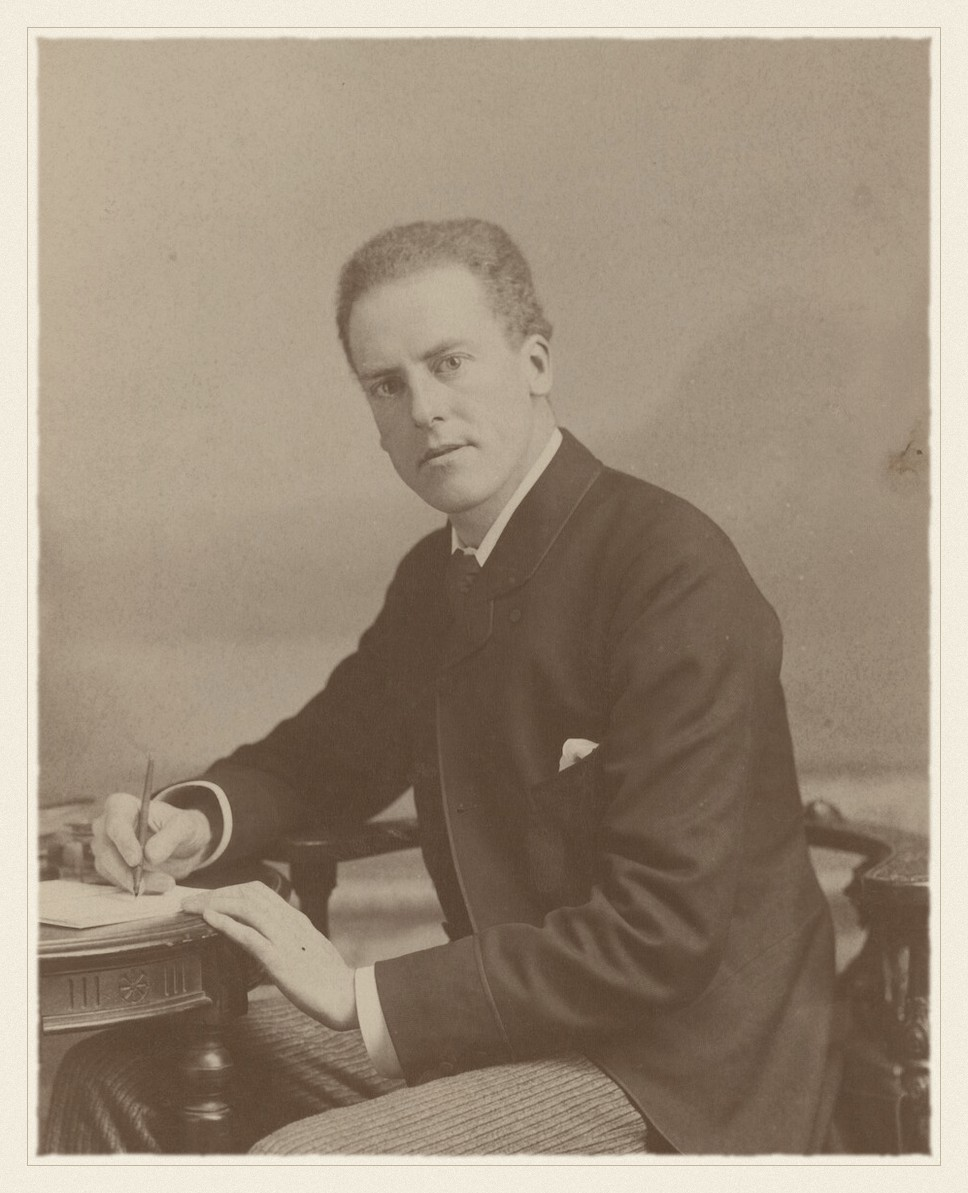
\includegraphics[keepaspectratio]{images/session-07-pearson.jpg}}

\textbf{Karl Pearson} · \textbf{1857--1936}

Principal components, 1901 --- lines and planes of closest fit.

{Elliott \& Fry, undated. Public domain, via Wikimedia Commons.}

\end{qmibplate}

\begin{qmibarchive}

\textbf{From the archive · Pearson, 1901}

Karl Pearson's paper is called \emph{On lines and planes of closest fit
to systems of points in space}, and the title contains the whole idea
(\citeproc{ref-pearson1901}{Pearson 1901}). He asked what line best fits
a cloud of points when there is no distinguished variable to predict ---
when \(x\) and \(y\) are on the same footing and the question is the
shape of the cloud rather than the conditional mean of one coordinate
given the other.

The answer differs from regression in a way worth seeing rather than
being told. Least squares minimises \emph{vertical} distances, because
it treats \(y\) as the thing to be explained and \(x\) as given.
Pearson's line minimises \emph{perpendicular} distances, because neither
coordinate is privileged. They are different lines, and the difference
grows as the correlation weakens.

Hotelling gave the method its modern algebra and its name three decades
later, deriving the components as the eigenvectors of the covariance
matrix and establishing that they successively capture maximal variance
(\citeproc{ref-hotelling1933}{Hotelling 1933}).

\begin{Shaded}
\begin{Highlighting}[]
\ImportTok{import}\NormalTok{ sys, warnings}
\NormalTok{sys.path.insert(}\DecValTok{0}\NormalTok{, }\StringTok{"../slides"}\NormalTok{)}\OperatorTok{;}\NormalTok{ sys.path.insert(}\DecValTok{0}\NormalTok{, }\StringTok{".."}\NormalTok{)}
\NormalTok{warnings.filterwarnings(}\StringTok{"ignore"}\NormalTok{)}
\ImportTok{from}\NormalTok{ plotstyle }\ImportTok{import}\NormalTok{ setup, CL}
\NormalTok{plt }\OperatorTok{=}\NormalTok{ setup()}

\ImportTok{import}\NormalTok{ numpy }\ImportTok{as}\NormalTok{ np, pandas }\ImportTok{as}\NormalTok{ pd, qmib}

\NormalTok{rng }\OperatorTok{=}\NormalTok{ np.random.default\_rng(}\DecValTok{60033}\NormalTok{)}
\NormalTok{n }\OperatorTok{=} \DecValTok{90}
\NormalTok{xs }\OperatorTok{=}\NormalTok{ rng.normal(}\DecValTok{0}\NormalTok{, }\DecValTok{1}\NormalTok{, n)}
\NormalTok{ys }\OperatorTok{=} \FloatTok{0.72} \OperatorTok{*}\NormalTok{ xs }\OperatorTok{+}\NormalTok{ rng.normal(}\DecValTok{0}\NormalTok{, }\FloatTok{0.72}\NormalTok{, n)}
\NormalTok{xs, ys }\OperatorTok{=}\NormalTok{ xs }\OperatorTok{{-}}\NormalTok{ xs.mean(), ys }\OperatorTok{{-}}\NormalTok{ ys.mean()}

\NormalTok{b\_reg }\OperatorTok{=}\NormalTok{ np.polyfit(xs, ys, }\DecValTok{1}\NormalTok{)[}\DecValTok{0}\NormalTok{]}
\NormalTok{M }\OperatorTok{=}\NormalTok{ np.column\_stack([xs, ys])}
\NormalTok{\_, \_, Vt }\OperatorTok{=}\NormalTok{ np.linalg.svd(M, full\_matrices}\OperatorTok{=}\VariableTok{False}\NormalTok{)}
\NormalTok{b\_pc }\OperatorTok{=}\NormalTok{ Vt[}\DecValTok{0}\NormalTok{, }\DecValTok{1}\NormalTok{] }\OperatorTok{/}\NormalTok{ Vt[}\DecValTok{0}\NormalTok{, }\DecValTok{0}\NormalTok{]}

\NormalTok{fig, ax }\OperatorTok{=}\NormalTok{ plt.subplots(figsize}\OperatorTok{=}\NormalTok{(}\FloatTok{6.2}\NormalTok{, }\FloatTok{4.8}\NormalTok{))}
\NormalTok{gx }\OperatorTok{=}\NormalTok{ np.linspace(xs.}\BuiltInTok{min}\NormalTok{() }\OperatorTok{*} \FloatTok{1.1}\NormalTok{, xs.}\BuiltInTok{max}\NormalTok{() }\OperatorTok{*} \FloatTok{1.1}\NormalTok{, }\DecValTok{40}\NormalTok{)}

\CommentTok{\# the residuals each method minimises}
\ControlFlowTok{for}\NormalTok{ xi, yi }\KeywordTok{in} \BuiltInTok{zip}\NormalTok{(xs, ys):}
\NormalTok{    ax.plot([xi, xi], [yi, b\_reg }\OperatorTok{*}\NormalTok{ xi], color}\OperatorTok{=}\NormalTok{CL.muted, lw}\OperatorTok{=}\FloatTok{0.6}\NormalTok{, alpha}\OperatorTok{=}\FloatTok{0.55}\NormalTok{, zorder}\OperatorTok{=}\DecValTok{1}\NormalTok{)}
\NormalTok{d }\OperatorTok{=}\NormalTok{ np.array([Vt[}\DecValTok{0}\NormalTok{, }\DecValTok{0}\NormalTok{], Vt[}\DecValTok{0}\NormalTok{, }\DecValTok{1}\NormalTok{]])}
\ControlFlowTok{for}\NormalTok{ xi, yi }\KeywordTok{in} \BuiltInTok{zip}\NormalTok{(xs, ys):}
\NormalTok{    proj }\OperatorTok{=}\NormalTok{ (np.array([xi, yi]) }\OperatorTok{@}\NormalTok{ d) }\OperatorTok{*}\NormalTok{ d}
\NormalTok{    ax.plot([xi, proj[}\DecValTok{0}\NormalTok{]], [yi, proj[}\DecValTok{1}\NormalTok{]], color}\OperatorTok{=}\NormalTok{CL.warn, lw}\OperatorTok{=}\FloatTok{0.6}\NormalTok{, alpha}\OperatorTok{=}\FloatTok{0.5}\NormalTok{, zorder}\OperatorTok{=}\DecValTok{1}\NormalTok{)}

\NormalTok{ax.plot(gx, b\_reg }\OperatorTok{*}\NormalTok{ gx, color}\OperatorTok{=}\NormalTok{CL.muted, lw}\OperatorTok{=}\FloatTok{2.2}\NormalTok{, label}\OperatorTok{=}\SpecialStringTok{f"regression  (slope }\SpecialCharTok{\{}\NormalTok{b\_reg}\SpecialCharTok{:.2f\}}\SpecialStringTok{)"}\NormalTok{)}
\NormalTok{ax.plot(gx, b\_pc }\OperatorTok{*}\NormalTok{ gx, color}\OperatorTok{=}\NormalTok{CL.warn, lw}\OperatorTok{=}\FloatTok{2.2}\NormalTok{, label}\OperatorTok{=}\SpecialStringTok{f"first component  (slope }\SpecialCharTok{\{}\NormalTok{b\_pc}\SpecialCharTok{:.2f\}}\SpecialStringTok{)"}\NormalTok{)}
\NormalTok{ax.scatter(xs, ys, s}\OperatorTok{=}\DecValTok{18}\NormalTok{, color}\OperatorTok{=}\NormalTok{CL.accent, alpha}\OperatorTok{=}\FloatTok{0.6}\NormalTok{, edgecolor}\OperatorTok{=}\StringTok{"none"}\NormalTok{, zorder}\OperatorTok{=}\DecValTok{3}\NormalTok{)}
\NormalTok{ax.set\_xlabel(}\StringTok{"x"}\NormalTok{)}\OperatorTok{;}\NormalTok{ ax.set\_ylabel(}\StringTok{"y"}\NormalTok{)}
\NormalTok{ax.legend(frameon}\OperatorTok{=}\VariableTok{False}\NormalTok{, fontsize}\OperatorTok{=}\FloatTok{8.5}\NormalTok{, loc}\OperatorTok{=}\StringTok{"upper left"}\NormalTok{)}
\NormalTok{ax.set\_aspect(}\StringTok{"equal"}\NormalTok{)}
\NormalTok{fig.tight\_layout()}
\end{Highlighting}
\end{Shaded}

\begin{figure}[htbp]

\centering{

\pandocbounded{
\includegraphics[keepaspectratio]{session-07_files/figure-pdf/fig-pearson-line-output-1.png}}

}

\caption{\label{fig-pearson-line}Regression and the first principal
component are not the same line. Least squares minimises the vertical
distances (grey); Pearson's line minimises the perpendicular ones (red).
The regression line is always the flatter of the two.}

\end{figure}%

\end{qmibarchive}

\section{Standardise, or the biggest units
win}\label{standardise-or-the-biggest-units-win}

PCA maximises variance, and variance has units. A variable measured in
hundreds of millions will have a variance many orders of magnitude
larger than one measured from zero to ten, and the first component will
therefore be, almost entirely, that variable. Nothing has been
discovered; the units have been reported back.

\phantomsection\label{check-standardise}
\begin{Shaded}
\begin{Highlighting}[]
\NormalTok{movies }\OperatorTok{=}\NormalTok{ qmib.load(}\StringTok{"movies"}\NormalTok{).select\_dtypes(}\StringTok{"number"}\NormalTok{).dropna()}

\CommentTok{\# A data{-}quality problem first — see the section at the end of this chapter.}
\NormalTok{usable }\OperatorTok{=}\NormalTok{ movies[(movies[}\StringTok{"budget"}\NormalTok{] }\OperatorTok{\textgreater{}} \DecValTok{0}\NormalTok{) }\OperatorTok{\&}\NormalTok{ (movies[}\StringTok{"revenue"}\NormalTok{] }\OperatorTok{\textgreater{}} \DecValTok{0}\NormalTok{)}
                \OperatorTok{\&}\NormalTok{ (movies[}\StringTok{"runtime"}\NormalTok{] }\OperatorTok{\textgreater{}} \DecValTok{0}\NormalTok{)].copy()}
\NormalTok{X }\OperatorTok{=}\NormalTok{ usable.to\_numpy(}\BuiltInTok{float}\NormalTok{)}
\NormalTok{cols }\OperatorTok{=} \BuiltInTok{list}\NormalTok{(usable.columns)}
\BuiltInTok{print}\NormalTok{(}\SpecialStringTok{f"rows used: }\SpecialCharTok{\{}\BuiltInTok{len}\NormalTok{(usable)}\SpecialCharTok{:,\}}\SpecialStringTok{ of }\SpecialCharTok{\{}\BuiltInTok{len}\NormalTok{(movies)}\SpecialCharTok{:,\}}\SpecialStringTok{"}\NormalTok{)}

\KeywordTok{def}\NormalTok{ eigen(A):}
\NormalTok{    ev, V }\OperatorTok{=}\NormalTok{ np.linalg.eigh(A)}
    \ControlFlowTok{return}\NormalTok{ ev[::}\OperatorTok{{-}}\DecValTok{1}\NormalTok{], V[:, ::}\OperatorTok{{-}}\DecValTok{1}\NormalTok{]}

\NormalTok{Xc }\OperatorTok{=}\NormalTok{ X }\OperatorTok{{-}}\NormalTok{ X.mean(}\DecValTok{0}\NormalTok{)}
\NormalTok{ev\_raw, V\_raw }\OperatorTok{=}\NormalTok{ eigen(np.cov(Xc, rowvar}\OperatorTok{=}\VariableTok{False}\NormalTok{))}
\BuiltInTok{print}\NormalTok{(}\SpecialStringTok{f"}\CharTok{\textbackslash{}n}\SpecialStringTok{RAW UNITS: first component captures }\SpecialCharTok{\{}\NormalTok{ev\_raw[}\DecValTok{0}\NormalTok{]}\OperatorTok{/}\NormalTok{ev\_raw}\SpecialCharTok{.}\BuiltInTok{sum}\NormalTok{()}\SpecialCharTok{:.2\%\}}\SpecialStringTok{ of variance"}\NormalTok{)}
\BuiltInTok{print}\NormalTok{(}\StringTok{"  its loadings:"}\NormalTok{)}
\ControlFlowTok{for}\NormalTok{ c, l }\KeywordTok{in} \BuiltInTok{sorted}\NormalTok{(}\BuiltInTok{zip}\NormalTok{(cols, V\_raw[:, }\DecValTok{0}\NormalTok{]), key}\OperatorTok{=}\KeywordTok{lambda}\NormalTok{ t: }\OperatorTok{{-}}\BuiltInTok{abs}\NormalTok{(t[}\DecValTok{1}\NormalTok{])):}
    \BuiltInTok{print}\NormalTok{(}\SpecialStringTok{f"    }\SpecialCharTok{\{}\NormalTok{c}\SpecialCharTok{:14\}\{}\NormalTok{l}\SpecialCharTok{:+8.4f\}}\SpecialStringTok{"}\NormalTok{)}

\NormalTok{Z }\OperatorTok{=}\NormalTok{ (X }\OperatorTok{{-}}\NormalTok{ X.mean(}\DecValTok{0}\NormalTok{)) }\OperatorTok{/}\NormalTok{ X.std(}\DecValTok{0}\NormalTok{, ddof}\OperatorTok{=}\DecValTok{1}\NormalTok{)}
\NormalTok{ev, V }\OperatorTok{=}\NormalTok{ eigen(np.corrcoef(Z, rowvar}\OperatorTok{=}\VariableTok{False}\NormalTok{))}
\BuiltInTok{print}\NormalTok{(}\SpecialStringTok{f"}\CharTok{\textbackslash{}n}\SpecialStringTok{STANDARDISED: first component captures }\SpecialCharTok{\{}\NormalTok{ev[}\DecValTok{0}\NormalTok{]}\OperatorTok{/}\NormalTok{ev}\SpecialCharTok{.}\BuiltInTok{sum}\NormalTok{()}\SpecialCharTok{:.2\%\}}\SpecialStringTok{"}\NormalTok{)}
\BuiltInTok{print}\NormalTok{(}\SpecialStringTok{f"  eigenvalues: }\SpecialCharTok{\{}\NormalTok{np}\SpecialCharTok{.}\BuiltInTok{round}\NormalTok{(ev, }\DecValTok{3}\NormalTok{)}\SpecialCharTok{\}}\SpecialStringTok{"}\NormalTok{)}
\end{Highlighting}
\end{Shaded}

\begin{verbatim}
rows used: 5,369 of 45,203

RAW UNITS: first component captures 97.50% of variance
  its loadings:
    revenue        -0.9840
    budget         -0.1783
    vote_count     -0.0000
    popularity     -0.0000
    runtime        -0.0000
    vote_average   -0.0000

STANDARDISED: first component captures 47.32%
  eigenvalues: [2.839 1.203 0.831 0.632 0.306 0.189]
\end{verbatim}

Ninety-seven and a half per cent of the variance on one component,
loading almost entirely on revenue, and it means nothing at all. Revenue
is measured in dollars and runtime in minutes; the analysis has ranked
the columns by the size of their units. Standardising each variable to
unit variance removes the arbitrariness, and it changes the answer
completely: the first component now captures under half the variance,
and there is a second worth looking at.

Standardisation is therefore part of the method rather than a
preliminary --- the same conclusion chapter 5 reached about the
penalties, for the same reason. The practical consequence is that PCA is
almost always performed on the \emph{correlation} matrix, which is the
covariance matrix of standardised data.

\section{How many components?}\label{how-many-components}

\begin{qmibdefinition}

{\textbf{Eigenvalue}} --- the variance of the data along a component. On
standardised data the eigenvalues sum to the number of variables, so an
eigenvalue of 1 corresponds to the variance of one original variable ---
a component that explains no more than a single column would have on its
own.

\end{qmibdefinition}

That gives the oldest rule: keep components with eigenvalue above 1. It
is a convention, not a test, and it is known to over-retain. Two better
instruments exist, and they disagree usefully.

Cattell's \emph{scree test} looks for the elbow: plot the eigenvalues in
order and retain those above the point where the curve flattens into
rubble (\citeproc{ref-cattell1966}{Cattell 1966}). It is subjective by
construction, which is a fair criticism and not a fatal one --- the
judgement is at least visible.

Horn's \emph{parallel analysis} makes it empirical
(\citeproc{ref-horn1965}{Horn 1965}). Generate data of the same shape
with no correlation at all, compute its eigenvalues, and retain only
components whose eigenvalue exceeds what pure noise of that size
produces. It answers the right question --- is this component larger
than chance --- and it is the method to use when you can.

\begin{Shaded}
\begin{Highlighting}[]
\NormalTok{n\_obs, n\_var }\OperatorTok{=}\NormalTok{ Z.shape}
\NormalTok{rng2 }\OperatorTok{=}\NormalTok{ np.random.default\_rng(}\DecValTok{7}\NormalTok{)}
\NormalTok{sim }\OperatorTok{=}\NormalTok{ np.array([np.linalg.eigvalsh(np.corrcoef(}
\NormalTok{    rng2.normal(size}\OperatorTok{=}\NormalTok{(n\_obs, n\_var)), rowvar}\OperatorTok{=}\VariableTok{False}\NormalTok{))[::}\OperatorTok{{-}}\DecValTok{1}\NormalTok{] }\ControlFlowTok{for}\NormalTok{ \_ }\KeywordTok{in} \BuiltInTok{range}\NormalTok{(}\DecValTok{200}\NormalTok{)])}
\NormalTok{noise\_95 }\OperatorTok{=}\NormalTok{ np.percentile(sim, }\DecValTok{95}\NormalTok{, axis}\OperatorTok{=}\DecValTok{0}\NormalTok{)}

\NormalTok{fig, ax }\OperatorTok{=}\NormalTok{ plt.subplots(figsize}\OperatorTok{=}\NormalTok{(}\FloatTok{6.6}\NormalTok{, }\FloatTok{4.2}\NormalTok{))}
\NormalTok{k }\OperatorTok{=}\NormalTok{ np.arange(}\DecValTok{1}\NormalTok{, n\_var }\OperatorTok{+} \DecValTok{1}\NormalTok{)}
\NormalTok{ax.plot(k, ev, marker}\OperatorTok{=}\StringTok{"o"}\NormalTok{, ms}\OperatorTok{=}\DecValTok{6}\NormalTok{, lw}\OperatorTok{=}\DecValTok{2}\NormalTok{, color}\OperatorTok{=}\NormalTok{CL.accent, label}\OperatorTok{=}\StringTok{"observed"}\NormalTok{, zorder}\OperatorTok{=}\DecValTok{3}\NormalTok{)}
\NormalTok{ax.plot(k, noise\_95, marker}\OperatorTok{=}\StringTok{"s"}\NormalTok{, ms}\OperatorTok{=}\DecValTok{4}\NormalTok{, lw}\OperatorTok{=}\FloatTok{1.5}\NormalTok{, ls}\OperatorTok{=}\StringTok{"{-}{-}"}\NormalTok{, color}\OperatorTok{=}\NormalTok{CL.warn,}
\NormalTok{        label}\OperatorTok{=}\StringTok{"95th percentile of uncorrelated data"}\NormalTok{, zorder}\OperatorTok{=}\DecValTok{2}\NormalTok{)}
\NormalTok{ax.axhline(}\FloatTok{1.0}\NormalTok{, color}\OperatorTok{=}\NormalTok{CL.muted, lw}\OperatorTok{=}\FloatTok{1.2}\NormalTok{, ls}\OperatorTok{=}\StringTok{":"}\NormalTok{, label}\OperatorTok{=}\StringTok{"Kaiser: eigenvalue = 1"}\NormalTok{)}
\NormalTok{ax.set\_xlabel(}\StringTok{"component"}\NormalTok{)}\OperatorTok{;}\NormalTok{ ax.set\_ylabel(}\StringTok{"eigenvalue"}\NormalTok{)}
\NormalTok{ax.set\_xticks(k)}
\NormalTok{ax.legend(frameon}\OperatorTok{=}\VariableTok{False}\NormalTok{, fontsize}\OperatorTok{=}\FloatTok{8.5}\NormalTok{)}
\NormalTok{fig.tight\_layout()}

\BuiltInTok{print}\NormalTok{(}\SpecialStringTok{f"Kaiser (\textgreater{}1):            retain }\SpecialCharTok{\{}\NormalTok{(ev }\OperatorTok{\textgreater{}} \DecValTok{1}\NormalTok{)}\SpecialCharTok{.}\BuiltInTok{sum}\NormalTok{()}\SpecialCharTok{\}}\SpecialStringTok{"}\NormalTok{)}
\BuiltInTok{print}\NormalTok{(}\SpecialStringTok{f"parallel analysis:      retain }\SpecialCharTok{\{}\NormalTok{(ev }\OperatorTok{\textgreater{}}\NormalTok{ noise\_95)}\SpecialCharTok{.}\BuiltInTok{sum}\NormalTok{()}\SpecialCharTok{\}}\SpecialStringTok{"}\NormalTok{)}
\BuiltInTok{print}\NormalTok{(}\SpecialStringTok{f"cumulative variance of the first two: }\SpecialCharTok{\{}\NormalTok{(ev[:}\DecValTok{2}\NormalTok{].}\BuiltInTok{sum}\NormalTok{()}\OperatorTok{/}\NormalTok{ev.}\BuiltInTok{sum}\NormalTok{())}\SpecialCharTok{:.1\%\}}\SpecialStringTok{"}\NormalTok{)}
\end{Highlighting}
\end{Shaded}

\begin{verbatim}
Kaiser (>1):            retain 2
parallel analysis:      retain 2
cumulative variance of the first two: 67.4%
\end{verbatim}

\begin{figure}[htbp]

\centering{

\pandocbounded{
\includegraphics[keepaspectratio]{session-07_files/figure-pdf/fig-scree-output-2.png}}

}

\caption{\label{fig-scree}Choosing the number of components three ways.
The Kaiser line at 1 retains two; the elbow suggests two; parallel
analysis against uncorrelated data of the same shape retains the
components lying above the dashed noise curve.}

\end{figure}%

\section{Loadings and scores are different
objects}\label{loadings-and-scores-are-different-objects}

The single most common confusion in applied use, and it has consequences
for what you are allowed to plot.

\begin{qmibdefinition}

{\textbf{Loading}} --- an element of the eigenvector: how much an
original \emph{variable} contributes to a component. There are as many
loadings per component as there are variables, and they describe what
the component \emph{means}.

\end{qmibdefinition}

\begin{qmibdefinition}

{\textbf{Score}} --- the value of a component for an \emph{observation},
computed as \(Z v_j\). There are as many scores per component as there
are rows, and they are the new coordinates you would use in a subsequent
regression.

\end{qmibdefinition}

Loadings interpret; scores are data. A biplot shows both at once and is
therefore the standard display, but the two are on different scales and
the relative lengths of the loading arrows are meaningful only against
each other.

\begin{Shaded}
\begin{Highlighting}[]
\NormalTok{scores }\OperatorTok{=}\NormalTok{ Z }\OperatorTok{@}\NormalTok{ V[:, :}\DecValTok{2}\NormalTok{]}

\NormalTok{fig, ax }\OperatorTok{=}\NormalTok{ plt.subplots(figsize}\OperatorTok{=}\NormalTok{(}\FloatTok{7.0}\NormalTok{, }\FloatTok{5.4}\NormalTok{))}
\NormalTok{ax.scatter(scores[:, }\DecValTok{0}\NormalTok{], scores[:, }\DecValTok{1}\NormalTok{], s}\OperatorTok{=}\DecValTok{6}\NormalTok{, color}\OperatorTok{=}\NormalTok{CL.accent, alpha}\OperatorTok{=}\FloatTok{0.18}\NormalTok{,}
\NormalTok{           edgecolor}\OperatorTok{=}\StringTok{"none"}\NormalTok{, zorder}\OperatorTok{=}\DecValTok{1}\NormalTok{)}
\NormalTok{scale }\OperatorTok{=}\NormalTok{ np.}\BuiltInTok{abs}\NormalTok{(scores).}\BuiltInTok{max}\NormalTok{() }\OperatorTok{*} \FloatTok{0.72}
\ControlFlowTok{for}\NormalTok{ j, name }\KeywordTok{in} \BuiltInTok{enumerate}\NormalTok{(cols):}
\NormalTok{    ax.arrow(}\DecValTok{0}\NormalTok{, }\DecValTok{0}\NormalTok{, V[j, }\DecValTok{0}\NormalTok{] }\OperatorTok{*}\NormalTok{ scale, V[j, }\DecValTok{1}\NormalTok{] }\OperatorTok{*}\NormalTok{ scale, color}\OperatorTok{=}\NormalTok{CL.warn,}
\NormalTok{             width}\OperatorTok{=}\FloatTok{0.004}\NormalTok{, head\_width}\OperatorTok{=}\FloatTok{0.10}\NormalTok{, alpha}\OperatorTok{=}\FloatTok{0.9}\NormalTok{, zorder}\OperatorTok{=}\DecValTok{3}\NormalTok{)}
\NormalTok{    ax.text(V[j, }\DecValTok{0}\NormalTok{] }\OperatorTok{*}\NormalTok{ scale }\OperatorTok{*} \FloatTok{1.12}\NormalTok{, V[j, }\DecValTok{1}\NormalTok{] }\OperatorTok{*}\NormalTok{ scale }\OperatorTok{*} \FloatTok{1.12}\NormalTok{, name,}
\NormalTok{            fontsize}\OperatorTok{=}\FloatTok{8.5}\NormalTok{, color}\OperatorTok{=}\NormalTok{CL.ink, ha}\OperatorTok{=}\StringTok{"center"}\NormalTok{, va}\OperatorTok{=}\StringTok{"center"}\NormalTok{, zorder}\OperatorTok{=}\DecValTok{4}\NormalTok{)}
\NormalTok{ax.axhline(}\DecValTok{0}\NormalTok{, color}\OperatorTok{=}\NormalTok{CL.line, lw}\OperatorTok{=}\DecValTok{1}\NormalTok{)}\OperatorTok{;}\NormalTok{ ax.axvline(}\DecValTok{0}\NormalTok{, color}\OperatorTok{=}\NormalTok{CL.line, lw}\OperatorTok{=}\DecValTok{1}\NormalTok{)}
\NormalTok{ax.set\_xlabel(}\SpecialStringTok{f"component 1 (}\SpecialCharTok{\{}\NormalTok{ev[}\DecValTok{0}\NormalTok{]}\OperatorTok{/}\NormalTok{ev}\SpecialCharTok{.}\BuiltInTok{sum}\NormalTok{()}\SpecialCharTok{:.1\%\}}\SpecialStringTok{ of variance)"}\NormalTok{)}
\NormalTok{ax.set\_ylabel(}\SpecialStringTok{f"component 2 (}\SpecialCharTok{\{}\NormalTok{ev[}\DecValTok{1}\NormalTok{]}\OperatorTok{/}\NormalTok{ev}\SpecialCharTok{.}\BuiltInTok{sum}\NormalTok{()}\SpecialCharTok{:.1\%\}}\SpecialStringTok{)"}\NormalTok{)}
\NormalTok{fig.tight\_layout()}

\BuiltInTok{print}\NormalTok{(}\StringTok{"loadings on the first two components:"}\NormalTok{)}
\BuiltInTok{print}\NormalTok{(}\SpecialStringTok{f"}\SpecialCharTok{\{}\StringTok{\textquotesingle{}variable\textquotesingle{}}\SpecialCharTok{:14\}\{}\StringTok{\textquotesingle{}PC1\textquotesingle{}}\SpecialCharTok{:\textgreater{}9\}\{}\StringTok{\textquotesingle{}PC2\textquotesingle{}}\SpecialCharTok{:\textgreater{}9\}}\SpecialStringTok{"}\NormalTok{)}
\ControlFlowTok{for}\NormalTok{ j, name }\KeywordTok{in} \BuiltInTok{enumerate}\NormalTok{(cols):}
    \BuiltInTok{print}\NormalTok{(}\SpecialStringTok{f"}\SpecialCharTok{\{}\NormalTok{name}\SpecialCharTok{:14\}\{}\NormalTok{V[j,}\DecValTok{0}\NormalTok{]}\SpecialCharTok{:+9.3f\}\{}\NormalTok{V[j,}\DecValTok{1}\NormalTok{]}\SpecialCharTok{:+9.3f\}}\SpecialStringTok{"}\NormalTok{)}
\end{Highlighting}
\end{Shaded}

\begin{verbatim}
loadings on the first two components:
variable            PC1      PC2
budget           -0.462   +0.298
popularity       -0.370   +0.078
revenue          -0.533   +0.182
runtime          -0.213   -0.605
vote_average     -0.207   -0.710
vote_count       -0.526   +0.023
\end{verbatim}

\begin{figure}[htbp]

\centering{

\pandocbounded{
\includegraphics[keepaspectratio]{session-07_files/figure-pdf/fig-biplot-output-2.png}}

}

\caption{\label{fig-biplot}The first two components. Points are scores
--- one per film. Arrows are loadings --- one per variable. The first
component orders films by overall scale and reach; the second separates
long, well-rated films from expensive, widely-voted ones.}

\end{figure}%

\section{PCA is not factor analysis}\label{pca-is-not-factor-analysis}

The two are distinguished by what they do with the variance that a
variable does not share with the others.

PCA decomposes \emph{all} the variance. Every component is a weighted
sum of the observed variables, so the components are defined whatever
the correlations are --- even if there are none, PCA returns six
components for six variables and simply reports eigenvalues near 1. It
is a rotation, and rotations are always available.

Factor analysis splits the variance in two. Each observed variable is
modelled as a combination of a few common factors plus something
specific to itself:

\[
x \;=\; \Lambda f + u,
\qquad
\operatorname{Var}(x) \;=\; \underbrace{\Lambda \Lambda^\top}_{\text{common}} + \underbrace{\Psi}_{\text{unique}},
\]

with \(\Psi\) diagonal. The model asserts that the \emph{correlations
between} variables are produced entirely by the common factors, and that
whatever is left is particular to each variable. That is a testable
claim: a set of correlations may be incompatible with any small number
of factors.

\begin{qmibdefinition}

{\textbf{Communality}} --- the share of a variable's variance explained
by the common factors, \(\sum_j \lambda_{ij}^2\). Its complement is the
\emph{uniqueness}. A variable with low communality does not belong to
the factor structure and is telling you so.

\end{qmibdefinition}

The practical difference: use PCA when the goal is to compress many
correlated columns into a few for prediction or display, and factor
analysis when you believe in a latent quantity and want to estimate it.
Spearman's original argument for a general factor of intelligence is the
founding example of the second (\citeproc{ref-spearman1904}{Spearman
1904}), and the tradition of using PCA where the question was really
factor-analytic is long and mostly unhelpful
(\citeproc{ref-fabrigar1999}{Fabrigar et al. 1999}).

\section{A factor is identified only up to
rotation}\label{a-factor-is-identified-only-up-to-rotation}

This is the deepest fact in the chapter and the one most often glossed.

If \(\Lambda\) reproduces the correlations, so does \(\Lambda R\) for
\emph{any} orthogonal matrix \(R\), because

\[
(\Lambda R)(\Lambda R)^\top \;=\; \Lambda R R^\top \Lambda^\top \;=\; \Lambda \Lambda^\top .
\]

The model fits exactly as well. Every communality is unchanged. Nothing
observable distinguishes them --- and yet the loadings, which is to say
the \emph{interpretation}, can be completely different. There is no
statistical basis for preferring one rotation; the choice is made on
grounds of interpretability, and rotation criteria such as varimax
formalise a preference for loadings that are large or near zero rather
than middling (\citeproc{ref-kaiser1958}{Kaiser 1958}).

\phantomsection\label{check-rotation}
\begin{Shaded}
\begin{Highlighting}[]
\ImportTok{from}\NormalTok{ sklearn.decomposition }\ImportTok{import}\NormalTok{ FactorAnalysis}
\ImportTok{from}\NormalTok{ sklearn.preprocessing }\ImportTok{import}\NormalTok{ StandardScaler}

\CommentTok{\# The car{-}attribute battery: fourteen rated features, ninety respondents.}
\NormalTok{cars }\OperatorTok{=}\NormalTok{ qmib.load(}\StringTok{"efa"}\NormalTok{).select\_dtypes(}\StringTok{"number"}\NormalTok{).dropna()}
\NormalTok{Zc }\OperatorTok{=}\NormalTok{ StandardScaler().fit\_transform(cars)}

\NormalTok{fa }\OperatorTok{=}\NormalTok{ FactorAnalysis(n\_components}\OperatorTok{=}\DecValTok{3}\NormalTok{, random\_state}\OperatorTok{=}\DecValTok{0}\NormalTok{).fit(Zc)}
\NormalTok{L }\OperatorTok{=}\NormalTok{ fa.components\_.T}


\KeywordTok{def}\NormalTok{ varimax(L, tol}\OperatorTok{=}\FloatTok{1e{-}6}\NormalTok{, iters}\OperatorTok{=}\DecValTok{200}\NormalTok{):}
    \CommentTok{"""Kaiser\textquotesingle{}s criterion, by the standard SVD iteration."""}
\NormalTok{    p, k }\OperatorTok{=}\NormalTok{ L.shape}
\NormalTok{    R, d }\OperatorTok{=}\NormalTok{ np.eye(k), }\FloatTok{0.0}
    \ControlFlowTok{for}\NormalTok{ \_ }\KeywordTok{in} \BuiltInTok{range}\NormalTok{(iters):}
\NormalTok{        d\_old, Lam }\OperatorTok{=}\NormalTok{ d, L }\OperatorTok{@}\NormalTok{ R}
\NormalTok{        B }\OperatorTok{=}\NormalTok{ L.T }\OperatorTok{@}\NormalTok{ (Lam}\OperatorTok{**}\DecValTok{3} \OperatorTok{{-}}\NormalTok{ Lam }\OperatorTok{@}\NormalTok{ np.diag(np.diag(Lam.T }\OperatorTok{@}\NormalTok{ Lam)) }\OperatorTok{/}\NormalTok{ p)}
\NormalTok{        u, s, vt }\OperatorTok{=}\NormalTok{ np.linalg.svd(B)}
\NormalTok{        R, d }\OperatorTok{=}\NormalTok{ u }\OperatorTok{@}\NormalTok{ vt, s.}\BuiltInTok{sum}\NormalTok{()}
        \ControlFlowTok{if}\NormalTok{ d\_old }\KeywordTok{and}\NormalTok{ d }\OperatorTok{/}\NormalTok{ d\_old }\OperatorTok{\textless{}} \DecValTok{1} \OperatorTok{+}\NormalTok{ tol:}
            \ControlFlowTok{break}
    \ControlFlowTok{return}\NormalTok{ L }\OperatorTok{@}\NormalTok{ R, R}


\NormalTok{Lr, R }\OperatorTok{=}\NormalTok{ varimax(L)}

\BuiltInTok{print}\NormalTok{(}\SpecialStringTok{f"n = }\SpecialCharTok{\{}\BuiltInTok{len}\NormalTok{(cars)}\SpecialCharTok{\}}\SpecialStringTok{, variables = }\SpecialCharTok{\{}\NormalTok{cars}\SpecialCharTok{.}\NormalTok{shape[}\DecValTok{1}\NormalTok{]}\SpecialCharTok{\}}\SpecialStringTok{, factors = 3}\CharTok{\textbackslash{}n}\SpecialStringTok{"}\NormalTok{)}
\BuiltInTok{print}\NormalTok{(}\SpecialStringTok{f"}\SpecialCharTok{\{}\StringTok{\textquotesingle{}\textquotesingle{}}\SpecialCharTok{:22\}\{}\StringTok{\textquotesingle{}unrotated\textquotesingle{}}\SpecialCharTok{:\textgreater{}14\}\{}\StringTok{\textquotesingle{}varimax\textquotesingle{}}\SpecialCharTok{:\textgreater{}14\}}\SpecialStringTok{"}\NormalTok{)}
\BuiltInTok{print}\NormalTok{(}\SpecialStringTok{f"}\SpecialCharTok{\{}\StringTok{\textquotesingle{}||Lambda Lambda\^{}T||\textquotesingle{}}\SpecialCharTok{:22\}\{}\NormalTok{np}\SpecialCharTok{.}\NormalTok{linalg}\SpecialCharTok{.}\NormalTok{norm(L }\OperatorTok{@}\NormalTok{ L.T)}\SpecialCharTok{:14.8f\}}\SpecialStringTok{"}
      \SpecialStringTok{f"}\SpecialCharTok{\{}\NormalTok{np}\SpecialCharTok{.}\NormalTok{linalg}\SpecialCharTok{.}\NormalTok{norm(Lr }\OperatorTok{@}\NormalTok{ Lr.T)}\SpecialCharTok{:14.8f\}}\SpecialStringTok{"}\NormalTok{)}
\BuiltInTok{print}\NormalTok{(}\SpecialStringTok{f"}\SpecialCharTok{\{}\StringTok{\textquotesingle{}sum of communalities\textquotesingle{}}\SpecialCharTok{:22\}\{}\NormalTok{(L}\OperatorTok{**}\DecValTok{2}\NormalTok{)}\SpecialCharTok{.}\BuiltInTok{sum}\NormalTok{()}\SpecialCharTok{:14.8f\}\{}\NormalTok{(Lr}\OperatorTok{**}\DecValTok{2}\NormalTok{)}\SpecialCharTok{.}\BuiltInTok{sum}\NormalTok{()}\SpecialCharTok{:14.8f\}}\SpecialStringTok{"}\NormalTok{)}
\BuiltInTok{print}\NormalTok{(}\SpecialStringTok{f"}\CharTok{\textbackslash{}n}\SpecialStringTok{R is orthogonal: ||R\textquotesingle{}R {-} I|| = }\SpecialCharTok{\{}\NormalTok{np}\SpecialCharTok{.}\NormalTok{linalg}\SpecialCharTok{.}\NormalTok{norm(R.T }\OperatorTok{@}\NormalTok{ R }\OperatorTok{{-}}\NormalTok{ np.eye(}\DecValTok{3}\NormalTok{))}\SpecialCharTok{:.2e\}}\SpecialStringTok{"}\NormalTok{)}
\BuiltInTok{print}\NormalTok{(}\StringTok{"}\CharTok{\textbackslash{}n}\StringTok{Identical fit. Now the interpretation:"}\NormalTok{)}
\NormalTok{tab }\OperatorTok{=}\NormalTok{ pd.DataFrame(Lr, index}\OperatorTok{=}\NormalTok{cars.columns)}
\ControlFlowTok{for}\NormalTok{ c }\KeywordTok{in}\NormalTok{ tab.columns:}
    \BuiltInTok{print}\NormalTok{(}\SpecialStringTok{f"  factor }\SpecialCharTok{\{}\NormalTok{c}\OperatorTok{+}\DecValTok{1}\SpecialCharTok{\}}\SpecialStringTok{: }\SpecialCharTok{\{}\StringTok{\textquotesingle{}, \textquotesingle{}}\SpecialCharTok{.}\NormalTok{join(tab[c].}\BuiltInTok{abs}\NormalTok{().nlargest(}\DecValTok{3}\NormalTok{).index)}\SpecialCharTok{\}}\SpecialStringTok{"}\NormalTok{)}
\end{Highlighting}
\end{Shaded}

\begin{verbatim}
n = 90, variables = 14, factors = 3

                           unrotated       varimax
||Lambda Lambda^T||       2.79837923    2.79837923
sum of communalities      4.56171180    4.56171180

R is orthogonal: ||R'R - I|| = 3.96e-16

Identical fit. Now the interpretation:
  factor 1: space_comfort, fuel_type, after_sales_service
  factor 2: resale_value, maintenance, fuel_efficiency
  factor 3: testimonials, color, fuel_efficiency
\end{verbatim}

Two solutions, the same fit to eight decimal places, and different
stories. If a paper reports rotated loadings without naming the
rotation, it has not reported its result.

\section{What you may not call the
components}\label{what-you-may-not-call-the-components}

A component is a weighted sum of variables that happens to capture
variance. It is not a thing, it has no units, and its sign is arbitrary
--- multiply an eigenvector by \(-1\) and it is still an eigenvector, so
``high on component 1'' can be reversed by a convention in the software.

The temptation is to name it anyway. The first component above loads
positively on budget, revenue, votes and popularity, so it is tempting
to call it \emph{commercial success} and then to treat that name as a
measurement. Three things are wrong with doing so.

\textbf{The name is an interpretation, not a finding.} It is your
reading of a loading pattern, and a different reader may propose a
different name that fits the same numbers.

\textbf{Naming invites reification.} Once ``commercial success'' has a
column, it gets used in regressions, and its coefficient gets discussed
as though the quantity existed independently of the six columns it was
built from.

\textbf{The component is sample-specific.} Add films, drop a variable,
or restrict to one decade, and the loadings move. A named factor should
be stable across reasonable perturbations, and that is checkable ---
refit on resamples and look.

The disciplined form is to say what the component \emph{is}: ``the first
principal component, which loads positively on all six variables and
most strongly on revenue and vote count, and accounts for 47\% of the
standardised variance''. That sentence is defensible. ``A film's
commercial success'' is a claim about the world.

\section{The zeros, which are not
zeros}\label{the-zeros-which-are-not-zeros}

One data-quality note, because it changes every number in this chapter
and it is invisible in a correlation matrix.

\phantomsection\label{check-zeros}
\begin{Shaded}
\begin{Highlighting}[]
\BuiltInTok{print}\NormalTok{(}\SpecialStringTok{f"}\SpecialCharTok{\{}\StringTok{\textquotesingle{}variable\textquotesingle{}}\SpecialCharTok{:14\}\{}\StringTok{\textquotesingle{}zeros\textquotesingle{}}\SpecialCharTok{:\textgreater{}10\}\{}\StringTok{\textquotesingle{}share\textquotesingle{}}\SpecialCharTok{:\textgreater{}9\}}\SpecialStringTok{"}\NormalTok{)}
\ControlFlowTok{for}\NormalTok{ c }\KeywordTok{in}\NormalTok{ movies.columns:}
\NormalTok{    z }\OperatorTok{=} \BuiltInTok{int}\NormalTok{((movies[c] }\OperatorTok{==} \DecValTok{0}\NormalTok{).}\BuiltInTok{sum}\NormalTok{())}
    \BuiltInTok{print}\NormalTok{(}\SpecialStringTok{f"}\SpecialCharTok{\{}\NormalTok{c}\SpecialCharTok{:14\}\{}\NormalTok{z}\SpecialCharTok{:\textgreater{}10,\}\{}\NormalTok{z}\OperatorTok{/}\BuiltInTok{len}\NormalTok{(movies)}\SpecialCharTok{:\textgreater{}9.1\%\}}\SpecialStringTok{"}\NormalTok{)}
\BuiltInTok{print}\NormalTok{(}\SpecialStringTok{f"}\CharTok{\textbackslash{}n}\SpecialStringTok{rows with budget, revenue and runtime all positive: "}
      \SpecialStringTok{f"}\SpecialCharTok{\{}\BuiltInTok{len}\NormalTok{(usable)}\SpecialCharTok{:,\}}\SpecialStringTok{ of }\SpecialCharTok{\{}\BuiltInTok{len}\NormalTok{(movies)}\SpecialCharTok{:,\}}\SpecialStringTok{ (}\SpecialCharTok{\{}\BuiltInTok{len}\NormalTok{(usable)}\OperatorTok{/}\BuiltInTok{len}\NormalTok{(movies)}\SpecialCharTok{:.1\%\}}\SpecialStringTok{)"}\NormalTok{)}
\end{Highlighting}
\end{Shaded}

\begin{verbatim}
variable           zeros    share
budget            36,323    80.4%
popularity            60     0.1%
revenue           37,801    83.6%
runtime            1,558     3.4%
vote_average       2,899     6.4%
vote_count         2,800     6.2%

rows with budget, revenue and runtime all positive: 5,369 of 45,203 (11.9%)
\end{verbatim}

Four out of five films in this dataset have a budget of exactly zero,
and five out of six have revenue of exactly zero. No film costs nothing.
These are missing values recorded as the number 0 --- which arithmetic
cannot distinguish from a measurement, so every mean, every correlation
and every eigenvalue computed on the full table is contaminated.

This is chapter 2's missingness section arriving with consequences. The
correlation matrix on the full data is not a weaker version of the
truth; it is a description of a mixture of films and non-observations.
Dropping to the 5,369 complete rows is the minimum defensible response,
and it is not neutral either: films with recorded budgets are larger,
better documented and more recent, so the analysis now describes that
subset. Say so.

\section{A short review of the
literature}\label{a-short-review-of-the-literature-5}

\begin{qmiblit}

Pearson (\citeproc{ref-pearson1901}{1901}) posed the problem
geometrically --- the best-fitting line and plane to a cloud of points,
minimising perpendicular rather than vertical distance --- and Hotelling
(\citeproc{ref-hotelling1933}{1933}) supplied the eigen-decomposition
and the name. The two papers are worth reading in sequence for how
differently the same method looks from a geometric and an algebraic
starting point.

Factor analysis has a separate origin in Spearman
(\citeproc{ref-spearman1904}{1904}), whose argument for a general factor
from correlations among school subjects established the model of
observed variables as combinations of unobserved ones. The distinction
from PCA was blurred almost immediately, and Fabrigar et al.
(\citeproc{ref-fabrigar1999}{1999}) documents how routinely PCA is
reported where the research question was factor-analytic, along with the
consequences.

On how many to retain, Cattell (\citeproc{ref-cattell1966}{1966})
introduced the scree test, whose subjectivity is its standard criticism
and its visible honesty; Horn (\citeproc{ref-horn1965}{1965}) replaced
the judgement with a comparison against uncorrelated data of the same
dimensions, which is the method used above and still the best available.

Kaiser (\citeproc{ref-kaiser1958}{1958}) gave rotation its dominant
criterion. The underlying indeterminacy --- that loadings are identified
only up to an orthogonal transformation --- is not a defect of any
method but a property of the model, and it means that the interpretive
step is a choice the analyst makes and must disclose.

\end{qmiblit}

\section{What to report}\label{what-to-report-5}

\begin{enumerate}
\def\labelenumi{\arabic{enumi}.}
\tightlist
\item
  \textbf{That the inputs were standardised}, and on what matrix the
  decomposition was performed. Without it the result is a ranking of
  measurement units.
\item
  \textbf{The full eigenvalue spectrum}, not only the retained ones, and
  the cumulative variance.
\item
  \textbf{How many components you kept and by what rule} --- with
  parallel analysis if you can, and the scree plot either way so the
  reader can disagree.
\item
  \textbf{Loadings, with the rotation named.} Unrotated, varimax,
  oblimin: they fit identically and mean different things.
\item
  \textbf{Communalities}, if the model is factor analysis. A variable
  the factors do not explain should be discussed, not silently retained.
\item
  \textbf{The description rather than the name.} What the component
  loads on, and how much variance it carries. If you must give it a
  label, mark it as a label.
\item
  \textbf{What the components are not.} They are not measurements, they
  have arbitrary sign, they are specific to this sample and these
  variables, and a regression using them as predictors inherits all of
  that.
\end{enumerate}

\bookmarksetup{startatroot}

\chapter{K-Nearest Neighbours and the Bias--Variance
Trade-off}\label{k-nearest-neighbours-and-the-biasvariance-trade-off}

\section{A method with no model}\label{a-method-with-no-model}

Every method so far has assumed a form. Least squares assumes a line,
logistic regression assumes a curve, and the penalties in chapter 5
assume the line is worth shrinking toward. Each assumption is a claim
that can be wrong, and chapter 3 was about detecting when it is.

Nearest neighbours makes no such claim. To predict for a new
observation, find the \(k\) observations in the training data closest to
it, and average their outcomes:

\[
\hat f(x_0) \;=\; \frac{1}{k} \sum_{i \in N_k(x_0)} y_i ,
\]

where \(N_k(x_0)\) is the set of the \(k\) nearest training points. For
a classification problem, take the majority vote instead. There is no
fitting stage, no coefficient, no optimisation --- the training data
\emph{is} the model.

This looks like getting something for nothing, and the chapter is about
what it actually costs. The method is not assumption-free; it has simply
moved its assumption. Averaging the neighbours presumes that the
function is smooth enough that points close in \(x\) have similar \(y\),
and it presumes you know what ``close'' means. Both presumptions can
fail badly, and neither shows up as a diagnostic plot.

\begin{qmibmuted}

No portrait accompanies this chapter. The method is due to Evelyn Fix
and Joseph Hodges, in a 1951 technical report for the US Air Force
School of Aviation Medicine that went unpublished for nearly forty years
(\citeproc{ref-fix1951}{Fix and Hodges 1989}), and no freely licensed
likeness of either author appears to exist. The convention this book
follows is a real portrait or none.

\end{qmibmuted}

\section{The floor nobody beats}\label{the-floor-nobody-beats}

Before asking how well a classifier does, ask how well anything could.

\begin{qmibdefinition}

{\textbf{Bayes classifier}} --- the rule that assigns each \(x\) to the
most probable class given \(x\): predict class \(j\) where
\(\Pr(Y = j \mid X = x)\) is largest. Its error rate, the \emph{Bayes
rate}, is the lowest achievable by any classifier whatsoever.

\end{qmibdefinition}

The proof is a one-liner: at each \(x\), any rule either picks the most
probable class or does not, and picking it minimises the chance of being
wrong there. Integrating over \(x\) gives the result.

The Bayes classifier is not a method, because computing it requires
\(\Pr(Y \mid X)\) --- which is the thing you are trying to estimate. Its
value is conceptual and it is considerable. \textbf{A non-zero Bayes
rate means that error is not evidence of a bad model.} If the outcome is
genuinely uncertain given the predictors, no amount of flexibility, data
or cleverness removes the remaining error, and a practitioner who keeps
adding complexity to chase it is chasing noise.

The regression analogue is the irreducible error \(\sigma^2\): the
variance of \(y\) around \(f(x)\), which no estimator of \(f\) can
touch. It appears explicitly in the decomposition below.

\section{Where prediction error comes
from}\label{where-prediction-error-comes-from}

Take a target \(y = f(x) + \varepsilon\) with
\(\operatorname{E}[\varepsilon] = 0\) and
\(\operatorname{Var}(\varepsilon) = \sigma^2\). Let \(\hat f\) be an
estimate built from a random training sample. The expected squared error
at a point \(x_0\), averaged over training samples and over the noise in
a new observation, splits into three:

\[
\operatorname{E}\big[(y_0 - \hat f(x_0))^2\big]
\;=\;
\underbrace{\sigma^2}_{\text{irreducible}}
\;+\;
\underbrace{\big(\operatorname{E}[\hat f(x_0)] - f(x_0)\big)^2}_{\text{bias}^2}
\;+\;
\underbrace{\operatorname{Var}\big(\hat f(x_0)\big)}_{\text{variance}} .
\]

Chapter 5 used the last two terms to argue for a biased estimator. Here
all three matter, and the first is the one that makes the others
meaningful: because \(\sigma^2 > 0\), the total error has a floor, and
the \emph{only} quantity a modeller controls is how the remaining budget
is split between bias and variance.

The words are worth being precise about. \textbf{Bias} is how far the
method's \emph{average} prediction is from the truth --- an error it
makes systematically, in every sample. \textbf{Variance} is how much the
prediction moves when the training sample changes --- an error it makes
differently each time. A rigid method has high bias and low variance; a
flexible one has the reverse.

For nearest neighbours, \(k\) is the dial. Small \(k\) averages few
points, follows the data closely, and changes a lot when the data
change: low bias, high variance. Large \(k\) averages many points,
smooths across regions where the truth differs, and barely moves between
samples: high bias, low variance.

The decomposition is usually presented as algebra and left there. It is
measurable, if you are willing to simulate a world whose truth you know.

\begin{Shaded}
\begin{Highlighting}[]
\ImportTok{import}\NormalTok{ sys, warnings}
\NormalTok{sys.path.insert(}\DecValTok{0}\NormalTok{, }\StringTok{"../slides"}\NormalTok{)}\OperatorTok{;}\NormalTok{ sys.path.insert(}\DecValTok{0}\NormalTok{, }\StringTok{".."}\NormalTok{)}
\NormalTok{warnings.filterwarnings(}\StringTok{"ignore"}\NormalTok{)}
\ImportTok{from}\NormalTok{ plotstyle }\ImportTok{import}\NormalTok{ setup, CL}
\NormalTok{plt }\OperatorTok{=}\NormalTok{ setup()}

\ImportTok{import}\NormalTok{ numpy }\ImportTok{as}\NormalTok{ np, pandas }\ImportTok{as}\NormalTok{ pd, qmib}
\ImportTok{from}\NormalTok{ sklearn.neighbors }\ImportTok{import}\NormalTok{ KNeighborsRegressor}

\NormalTok{rng }\OperatorTok{=}\NormalTok{ np.random.default\_rng(}\DecValTok{60033}\NormalTok{)}

\KeywordTok{def}\NormalTok{ truth\_fn(x):}
    \ControlFlowTok{return}\NormalTok{ np.sin(}\DecValTok{2} \OperatorTok{*}\NormalTok{ np.pi }\OperatorTok{*}\NormalTok{ x) }\OperatorTok{+} \FloatTok{0.5} \OperatorTok{*}\NormalTok{ x}

\NormalTok{SIGMA, N, REPS }\OperatorTok{=} \FloatTok{0.35}\NormalTok{, }\DecValTok{120}\NormalTok{, }\DecValTok{400}
\NormalTok{x\_test }\OperatorTok{=}\NormalTok{ np.linspace(}\FloatTok{0.05}\NormalTok{, }\FloatTok{0.95}\NormalTok{, }\DecValTok{60}\NormalTok{).reshape(}\OperatorTok{{-}}\DecValTok{1}\NormalTok{, }\DecValTok{1}\NormalTok{)}
\NormalTok{f\_true }\OperatorTok{=}\NormalTok{ truth\_fn(x\_test.ravel())}

\NormalTok{ks }\OperatorTok{=}\NormalTok{ [}\DecValTok{1}\NormalTok{, }\DecValTok{2}\NormalTok{, }\DecValTok{3}\NormalTok{, }\DecValTok{5}\NormalTok{, }\DecValTok{8}\NormalTok{, }\DecValTok{12}\NormalTok{, }\DecValTok{20}\NormalTok{, }\DecValTok{30}\NormalTok{, }\DecValTok{45}\NormalTok{, }\DecValTok{60}\NormalTok{, }\DecValTok{80}\NormalTok{]}
\NormalTok{rows }\OperatorTok{=}\NormalTok{ []}
\ControlFlowTok{for}\NormalTok{ k }\KeywordTok{in}\NormalTok{ ks:}
\NormalTok{    preds }\OperatorTok{=}\NormalTok{ np.empty((REPS, }\BuiltInTok{len}\NormalTok{(x\_test)))}
\NormalTok{    mses }\OperatorTok{=}\NormalTok{ np.empty(REPS)}
    \ControlFlowTok{for}\NormalTok{ r }\KeywordTok{in} \BuiltInTok{range}\NormalTok{(REPS):}
\NormalTok{        xs }\OperatorTok{=}\NormalTok{ rng.uniform(}\DecValTok{0}\NormalTok{, }\DecValTok{1}\NormalTok{, N).reshape(}\OperatorTok{{-}}\DecValTok{1}\NormalTok{, }\DecValTok{1}\NormalTok{)}
\NormalTok{        ys }\OperatorTok{=}\NormalTok{ truth\_fn(xs.ravel()) }\OperatorTok{+}\NormalTok{ rng.normal(}\DecValTok{0}\NormalTok{, SIGMA, N)}
\NormalTok{        preds[r] }\OperatorTok{=}\NormalTok{ KNeighborsRegressor(n\_neighbors}\OperatorTok{=}\NormalTok{k).fit(xs, ys).predict(x\_test)}
\NormalTok{        mses[r] }\OperatorTok{=}\NormalTok{ np.mean((f\_true }\OperatorTok{+}\NormalTok{ rng.normal(}\DecValTok{0}\NormalTok{, SIGMA, }\BuiltInTok{len}\NormalTok{(x\_test)) }\OperatorTok{{-}}\NormalTok{ preds[r]) }\OperatorTok{**} \DecValTok{2}\NormalTok{)}
\NormalTok{    rows.append(}\BuiltInTok{dict}\NormalTok{(k}\OperatorTok{=}\NormalTok{k,}
\NormalTok{                     bias2}\OperatorTok{=}\NormalTok{np.mean((preds.mean(}\DecValTok{0}\NormalTok{) }\OperatorTok{{-}}\NormalTok{ f\_true) }\OperatorTok{**} \DecValTok{2}\NormalTok{),}
\NormalTok{                     var}\OperatorTok{=}\NormalTok{np.mean(preds.var(}\DecValTok{0}\NormalTok{)),}
\NormalTok{                     mse}\OperatorTok{=}\NormalTok{mses.mean()))}

\NormalTok{bv }\OperatorTok{=}\NormalTok{ pd.DataFrame(rows)}
\NormalTok{bv[}\StringTok{"total"}\NormalTok{] }\OperatorTok{=}\NormalTok{ bv.bias2 }\OperatorTok{+}\NormalTok{ bv[}\StringTok{"var"}\NormalTok{] }\OperatorTok{+}\NormalTok{ SIGMA }\OperatorTok{**} \DecValTok{2}

\NormalTok{fig, ax }\OperatorTok{=}\NormalTok{ plt.subplots(figsize}\OperatorTok{=}\NormalTok{(}\FloatTok{7.2}\NormalTok{, }\FloatTok{4.6}\NormalTok{))}
\NormalTok{ax.plot(bv.k, bv.bias2, marker}\OperatorTok{=}\StringTok{"o"}\NormalTok{, ms}\OperatorTok{=}\DecValTok{4}\NormalTok{, lw}\OperatorTok{=}\FloatTok{1.8}\NormalTok{, color}\OperatorTok{=}\NormalTok{CL.warn, label}\OperatorTok{=}\StringTok{"bias$\^{}2$"}\NormalTok{)}
\NormalTok{ax.plot(bv.k, bv[}\StringTok{"var"}\NormalTok{], marker}\OperatorTok{=}\StringTok{"s"}\NormalTok{, ms}\OperatorTok{=}\DecValTok{4}\NormalTok{, lw}\OperatorTok{=}\FloatTok{1.8}\NormalTok{, color}\OperatorTok{=}\NormalTok{CL.accent, label}\OperatorTok{=}\StringTok{"variance"}\NormalTok{)}
\NormalTok{ax.axhline(SIGMA }\OperatorTok{**} \DecValTok{2}\NormalTok{, ls}\OperatorTok{=}\StringTok{":"}\NormalTok{, lw}\OperatorTok{=}\FloatTok{1.4}\NormalTok{, color}\OperatorTok{=}\NormalTok{CL.muted, label}\OperatorTok{=}\VerbatimStringTok{r"irreducible }\DecValTok{$\textbackslash{}s}\VerbatimStringTok{igma}\DecValTok{\^{}}\VerbatimStringTok{2}\DecValTok{$}\VerbatimStringTok{"}\NormalTok{)}
\NormalTok{ax.plot(bv.k, bv.total, marker}\OperatorTok{=}\StringTok{"\^{}"}\NormalTok{, ms}\OperatorTok{=}\DecValTok{4}\NormalTok{, lw}\OperatorTok{=}\FloatTok{2.2}\NormalTok{, color}\OperatorTok{=}\NormalTok{CL.ink, label}\OperatorTok{=}\StringTok{"sum"}\NormalTok{)}
\NormalTok{ax.plot(bv.k, bv.mse, ls}\OperatorTok{=}\StringTok{"{-}{-}"}\NormalTok{, lw}\OperatorTok{=}\FloatTok{1.4}\NormalTok{, color}\OperatorTok{=}\NormalTok{CL.good, label}\OperatorTok{=}\StringTok{"measured test MSE"}\NormalTok{)}
\NormalTok{best }\OperatorTok{=}\NormalTok{ bv.loc[bv.total.idxmin(), }\StringTok{"k"}\NormalTok{]}
\NormalTok{ax.axvline(best, color}\OperatorTok{=}\NormalTok{CL.muted, lw}\OperatorTok{=}\DecValTok{1}\NormalTok{, alpha}\OperatorTok{=}\FloatTok{0.6}\NormalTok{)}
\NormalTok{ax.set\_xlabel(}\StringTok{"$k$"}\NormalTok{)}\OperatorTok{;}\NormalTok{ ax.set\_ylabel(}\StringTok{"expected squared error"}\NormalTok{)}
\NormalTok{ax.set\_xscale(}\StringTok{"log"}\NormalTok{)}\OperatorTok{;}\NormalTok{ ax.set\_xticks(ks)}\OperatorTok{;}\NormalTok{ ax.set\_xticklabels(ks)}
\NormalTok{ax.legend(frameon}\OperatorTok{=}\VariableTok{False}\NormalTok{, fontsize}\OperatorTok{=}\FloatTok{8.5}\NormalTok{)}
\NormalTok{fig.tight\_layout()}

\BuiltInTok{print}\NormalTok{(}\SpecialStringTok{f"}\SpecialCharTok{\{}\StringTok{\textquotesingle{}k\textquotesingle{}}\SpecialCharTok{:\textgreater{}4\}\{}\StringTok{\textquotesingle{}bias²\textquotesingle{}}\SpecialCharTok{:\textgreater{}10\}\{}\StringTok{\textquotesingle{}variance\textquotesingle{}}\SpecialCharTok{:\textgreater{}11\}\{}\StringTok{\textquotesingle{}σ²\textquotesingle{}}\SpecialCharTok{:\textgreater{}9\}\{}\StringTok{\textquotesingle{}sum\textquotesingle{}}\SpecialCharTok{:\textgreater{}10\}\{}\StringTok{\textquotesingle{}test MSE\textquotesingle{}}\SpecialCharTok{:\textgreater{}11\}}\SpecialStringTok{"}\NormalTok{)}
\ControlFlowTok{for}\NormalTok{ \_, r }\KeywordTok{in}\NormalTok{ bv.iterrows():}
    \BuiltInTok{print}\NormalTok{(}\SpecialStringTok{f"}\SpecialCharTok{\{}\BuiltInTok{int}\NormalTok{(r.k)}\SpecialCharTok{:\textgreater{}4\}\{}\NormalTok{r}\SpecialCharTok{.}\NormalTok{bias2}\SpecialCharTok{:10.5f\}\{}\NormalTok{r[}\StringTok{\textquotesingle{}var\textquotesingle{}}\NormalTok{]}\SpecialCharTok{:11.5f\}\{}\NormalTok{SIGMA}\OperatorTok{**}\DecValTok{2}\SpecialCharTok{:9.5f\}}\SpecialStringTok{"}
          \SpecialStringTok{f"}\SpecialCharTok{\{}\NormalTok{r}\SpecialCharTok{.}\NormalTok{total}\SpecialCharTok{:10.5f\}\{}\NormalTok{r}\SpecialCharTok{.}\NormalTok{mse}\SpecialCharTok{:11.5f\}}\SpecialStringTok{"}\NormalTok{)}
\BuiltInTok{print}\NormalTok{(}\SpecialStringTok{f"}\CharTok{\textbackslash{}n}\SpecialStringTok{minimum total error at k = }\SpecialCharTok{\{}\BuiltInTok{int}\NormalTok{(best)}\SpecialCharTok{\}}\SpecialStringTok{"}\NormalTok{)}
\end{Highlighting}
\end{Shaded}

\begin{verbatim}
   k     bias²   variance       σ²       sum   test MSE
   1   0.00023    0.12467  0.12250   0.24741    0.24868
   2   0.00014    0.06256  0.12250   0.18520    0.18548
   3   0.00009    0.04060  0.12250   0.16318    0.16148
   5   0.00006    0.02551  0.12250   0.14807    0.14673
   8   0.00011    0.01625  0.12250   0.13886    0.14049
  12   0.00032    0.01164  0.12250   0.13446    0.13424
  20   0.00307    0.00889  0.12250   0.13446    0.13501
  30   0.01376    0.00769  0.12250   0.14395    0.14445
  45   0.03776    0.00673  0.12250   0.16699    0.16619
  60   0.06789    0.00666  0.12250   0.19705    0.19732
  80   0.16629    0.00783  0.12250   0.29661    0.29528

minimum total error at k = 12
\end{verbatim}

\begin{figure}[htbp]

\centering{

\pandocbounded{
\includegraphics[keepaspectratio]{session-08_files/figure-pdf/fig-bias-variance-output-2.png}}

}

\caption{\label{fig-bias-variance}The decomposition, measured. Four
hundred training samples are drawn from a known function; for each \(k\)
the squared bias and the variance of the prediction are computed across
samples. Their sum plus the irreducible error tracks the test error to
within 0.002 everywhere.}

\end{figure}%

Read the table rather than the shape. Variance falls by a factor of
sixteen between \(k = 1\) and \(k = 80\); squared bias rises by a factor
of several hundred. The sum is U-shaped with a minimum in between, and
the identity holds --- the sum of the three estimated components matches
the independently measured test error at every \(k\). That is the
decomposition being \emph{verified}, not illustrated.

Note also what happens at the extremes. At \(k = 1\) the method has
essentially no bias and all the error is variance plus noise. At
\(k = 80\), two thirds of the sample is averaged into every prediction
and the bias dominates. Neither extreme is a modelling failure; both are
the same dial at different settings.

\begin{qmibdefinition}

{\textbf{Effective degrees of freedom}} --- for \(k\)-nearest
neighbours, roughly \(n/k\). At \(k = 1\) the method has as many
effective parameters as observations, which is why it interpolates the
training data exactly; at \(k = n\) it has one, and predicts the global
mean everywhere. It is the same quantity chapter 5's penalty controlled
continuously.

\end{qmibdefinition}

\section{Distance is not given, it is
chosen}\label{distance-is-not-given-it-is-chosen}

Nearest neighbours needs a definition of ``near''. The default is
Euclidean distance,

\[
d(x_0, x_i) \;=\; \sqrt{\textstyle\sum_{j=1}^{p} (x_{0j} - x_{ij})^2},
\]

and that formula adds squared differences measured in different units. A
difference of one euro and a difference of one index point are treated
as identical quantities. In practice the variable with the largest
numerical range determines the neighbours entirely, and every other
predictor is decoration.

This is the third time this book has reached the same conclusion --- PCA
in chapter 7, the penalties in chapter 5, and now here --- and the
reason is always the same: any method that compares magnitudes across
variables must first make them comparable. \textbf{Standardise before
computing a distance.} The alternative is a method whose answer depends
on whether you recorded revenue in dollars or millions of dollars.

\section{The curse of dimensionality}\label{the-curse-of-dimensionality}

The deeper problem is that ``near'' stops existing as the number of
predictors grows, and it does so much faster than intuition suggests.

\phantomsection\label{check-curse}
\begin{Shaded}
\begin{Highlighting}[]
\NormalTok{rng2 }\OperatorTok{=}\NormalTok{ np.random.default\_rng(}\DecValTok{7}\NormalTok{)}
\BuiltInTok{print}\NormalTok{(}\SpecialStringTok{f"}\SpecialCharTok{\{}\StringTok{\textquotesingle{}dimensions\textquotesingle{}}\SpecialCharTok{:\textgreater{}11\}\{}\StringTok{\textquotesingle{}nearest\textquotesingle{}}\SpecialCharTok{:\textgreater{}10\}\{}\StringTok{\textquotesingle{}farthest\textquotesingle{}}\SpecialCharTok{:\textgreater{}10\}\{}\StringTok{\textquotesingle{}contrast\textquotesingle{}}\SpecialCharTok{:\textgreater{}11\}}\SpecialStringTok{"}\NormalTok{)}
\ControlFlowTok{for}\NormalTok{ p }\KeywordTok{in}\NormalTok{ [}\DecValTok{1}\NormalTok{, }\DecValTok{2}\NormalTok{, }\DecValTok{5}\NormalTok{, }\DecValTok{10}\NormalTok{, }\DecValTok{25}\NormalTok{, }\DecValTok{50}\NormalTok{, }\DecValTok{100}\NormalTok{, }\DecValTok{500}\NormalTok{]:}
\NormalTok{    X }\OperatorTok{=}\NormalTok{ rng2.uniform(}\DecValTok{0}\NormalTok{, }\DecValTok{1}\NormalTok{, (}\DecValTok{500}\NormalTok{, p))}
\NormalTok{    q }\OperatorTok{=}\NormalTok{ rng2.uniform(}\DecValTok{0}\NormalTok{, }\DecValTok{1}\NormalTok{, (}\DecValTok{1}\NormalTok{, p))}
\NormalTok{    dist }\OperatorTok{=}\NormalTok{ np.sqrt(((X }\OperatorTok{{-}}\NormalTok{ q) }\OperatorTok{**} \DecValTok{2}\NormalTok{).}\BuiltInTok{sum}\NormalTok{(axis}\OperatorTok{=}\DecValTok{1}\NormalTok{))}
    \BuiltInTok{print}\NormalTok{(}\SpecialStringTok{f"}\SpecialCharTok{\{}\NormalTok{p}\SpecialCharTok{:\textgreater{}11\}\{}\NormalTok{dist}\SpecialCharTok{.}\BuiltInTok{min}\NormalTok{()}\SpecialCharTok{:10.3f\}\{}\NormalTok{dist}\SpecialCharTok{.}\BuiltInTok{max}\NormalTok{()}\SpecialCharTok{:10.3f\}}\SpecialStringTok{"}
          \SpecialStringTok{f"}\SpecialCharTok{\{}\NormalTok{(dist.}\BuiltInTok{max}\NormalTok{() }\OperatorTok{{-}}\NormalTok{ dist.}\BuiltInTok{min}\NormalTok{())}\OperatorTok{/}\NormalTok{dist}\SpecialCharTok{.}\BuiltInTok{min}\NormalTok{()}\SpecialCharTok{:11.3f\}}\SpecialStringTok{"}\NormalTok{)}
\end{Highlighting}
\end{Shaded}

\begin{verbatim}
 dimensions   nearest  farthest   contrast
          1     0.000     0.579   1495.857
          2     0.036     1.129     30.482
          5     0.201     1.335      5.650
         10     0.665     1.842      1.769
         25     1.358     2.779      1.046
         50     2.319     3.559      0.535
        100     3.236     4.601      0.422
        500     8.126     9.851      0.212
\end{verbatim}

The last column is what matters: the gap between the nearest and the
farthest point, relative to the nearest. In one dimension the farthest
point is around a thousand times further away than the nearest. By fifty
dimensions it is half again as far; by five hundred, a fifth. All the
points are approximately the same distance from the query, so ``the ten
nearest'' is close to a random selection of ten
(\citeproc{ref-beyer1999}{Beyer et al. 1999}).

There is a second, geometric way to see the same thing. To capture a
fixed fraction \(r\) of the data in a hypercube of \(p\) dimensions, the
neighbourhood must span \(r^{1/p}\) of the range of \emph{each}
variable. Capturing 1\% of the data needs 10\% of the range in two
dimensions, 63\% in ten, and 95\% in a hundred --- a ``neighbourhood''
covering almost the entire space, which is not local in any useful
sense.

The consequence for practice is blunt. Nearest neighbours works well
with few predictors and abundant data, and degrades quickly as
predictors are added. Adding a variable to a linear model costs one
parameter; adding one to a nearest neighbour method costs a dimension of
the space in which distance must remain meaningful.

\section{\texorpdfstring{Choosing \(k\), and why training error
lies}{Choosing k, and why training error lies}}\label{choosing-k-and-why-training-error-lies}

The training error of \(1\)-nearest-neighbour is exactly zero: every
training point is its own nearest neighbour, so it predicts itself
perfectly. That number is not a measure of anything, and any procedure
that selects \(k\) by fitting error will select \(k = 1\) every time.

Cross-validation is the answer, as it was in chapter 5. Split, fit on
the rest, measure on the held-out part, rotate.

\begin{Shaded}
\begin{Highlighting}[]
\ImportTok{from}\NormalTok{ sklearn.model\_selection }\ImportTok{import}\NormalTok{ cross\_val\_score, KFold}

\NormalTok{xs }\OperatorTok{=}\NormalTok{ rng.uniform(}\DecValTok{0}\NormalTok{, }\DecValTok{1}\NormalTok{, }\DecValTok{200}\NormalTok{).reshape(}\OperatorTok{{-}}\DecValTok{1}\NormalTok{, }\DecValTok{1}\NormalTok{)}
\NormalTok{ys }\OperatorTok{=}\NormalTok{ truth\_fn(xs.ravel()) }\OperatorTok{+}\NormalTok{ rng.normal(}\DecValTok{0}\NormalTok{, SIGMA, }\DecValTok{200}\NormalTok{)}
\NormalTok{grid }\OperatorTok{=}\NormalTok{ [}\DecValTok{1}\NormalTok{, }\DecValTok{2}\NormalTok{, }\DecValTok{3}\NormalTok{, }\DecValTok{5}\NormalTok{, }\DecValTok{8}\NormalTok{, }\DecValTok{12}\NormalTok{, }\DecValTok{20}\NormalTok{, }\DecValTok{30}\NormalTok{, }\DecValTok{45}\NormalTok{, }\DecValTok{60}\NormalTok{, }\DecValTok{90}\NormalTok{, }\DecValTok{130}\NormalTok{]}

\NormalTok{train\_err, cv\_err }\OperatorTok{=}\NormalTok{ [], []}
\ControlFlowTok{for}\NormalTok{ k }\KeywordTok{in}\NormalTok{ grid:}
\NormalTok{    m }\OperatorTok{=}\NormalTok{ KNeighborsRegressor(n\_neighbors}\OperatorTok{=}\NormalTok{k).fit(xs, ys)}
\NormalTok{    train\_err.append(np.mean((ys }\OperatorTok{{-}}\NormalTok{ m.predict(xs)) }\OperatorTok{**} \DecValTok{2}\NormalTok{))}
\NormalTok{    cv\_err.append(}\OperatorTok{{-}}\NormalTok{cross\_val\_score(KNeighborsRegressor(n\_neighbors}\OperatorTok{=}\NormalTok{k), xs, ys,}
\NormalTok{                                   cv}\OperatorTok{=}\NormalTok{KFold(}\DecValTok{10}\NormalTok{, shuffle}\OperatorTok{=}\VariableTok{True}\NormalTok{, random\_state}\OperatorTok{=}\DecValTok{0}\NormalTok{),}
\NormalTok{                                   scoring}\OperatorTok{=}\StringTok{"neg\_mean\_squared\_error"}\NormalTok{).mean())}

\NormalTok{fig, ax }\OperatorTok{=}\NormalTok{ plt.subplots(figsize}\OperatorTok{=}\NormalTok{(}\FloatTok{7.0}\NormalTok{, }\FloatTok{4.3}\NormalTok{))}
\NormalTok{ax.plot(grid, train\_err, marker}\OperatorTok{=}\StringTok{"o"}\NormalTok{, ms}\OperatorTok{=}\DecValTok{4}\NormalTok{, lw}\OperatorTok{=}\FloatTok{1.8}\NormalTok{, color}\OperatorTok{=}\NormalTok{CL.muted, label}\OperatorTok{=}\StringTok{"training error"}\NormalTok{)}
\NormalTok{ax.plot(grid, cv\_err, marker}\OperatorTok{=}\StringTok{"s"}\NormalTok{, ms}\OperatorTok{=}\DecValTok{4}\NormalTok{, lw}\OperatorTok{=}\FloatTok{2.0}\NormalTok{, color}\OperatorTok{=}\NormalTok{CL.accent, label}\OperatorTok{=}\StringTok{"10{-}fold CV error"}\NormalTok{)}
\NormalTok{ax.axhline(SIGMA }\OperatorTok{**} \DecValTok{2}\NormalTok{, ls}\OperatorTok{=}\StringTok{":"}\NormalTok{, lw}\OperatorTok{=}\FloatTok{1.4}\NormalTok{, color}\OperatorTok{=}\NormalTok{CL.warn, label}\OperatorTok{=}\VerbatimStringTok{r"irreducible }\DecValTok{$\textbackslash{}s}\VerbatimStringTok{igma}\DecValTok{\^{}}\VerbatimStringTok{2}\DecValTok{$}\VerbatimStringTok{"}\NormalTok{)}
\NormalTok{ax.axvline(grid[}\BuiltInTok{int}\NormalTok{(np.argmin(cv\_err))], color}\OperatorTok{=}\NormalTok{CL.ink, lw}\OperatorTok{=}\DecValTok{1}\NormalTok{, ls}\OperatorTok{=}\StringTok{"{-}{-}"}\NormalTok{)}
\NormalTok{ax.set\_xlabel(}\StringTok{"$k$"}\NormalTok{)}\OperatorTok{;}\NormalTok{ ax.set\_ylabel(}\StringTok{"mean squared error"}\NormalTok{)}
\NormalTok{ax.set\_xscale(}\StringTok{"log"}\NormalTok{)}\OperatorTok{;}\NormalTok{ ax.set\_xticks(grid)}\OperatorTok{;}\NormalTok{ ax.set\_xticklabels(grid)}
\NormalTok{ax.legend(frameon}\OperatorTok{=}\VariableTok{False}\NormalTok{, fontsize}\OperatorTok{=}\FloatTok{8.5}\NormalTok{)}
\NormalTok{fig.tight\_layout()}

\BuiltInTok{print}\NormalTok{(}\SpecialStringTok{f"training error at k=1: }\SpecialCharTok{\{}\NormalTok{train\_err[}\DecValTok{0}\NormalTok{]}\SpecialCharTok{:.6f\}}\SpecialStringTok{  (exactly zero — every point is its own neighbour)"}\NormalTok{)}
\BuiltInTok{print}\NormalTok{(}\SpecialStringTok{f"CV chooses k = }\SpecialCharTok{\{}\NormalTok{grid[}\BuiltInTok{int}\NormalTok{(np.argmin(cv\_err))]}\SpecialCharTok{\}}\SpecialStringTok{, CV error }\SpecialCharTok{\{}\BuiltInTok{min}\NormalTok{(cv\_err)}\SpecialCharTok{:.4f\}}\SpecialStringTok{"}\NormalTok{)}
\BuiltInTok{print}\NormalTok{(}\SpecialStringTok{f"irreducible floor σ² = }\SpecialCharTok{\{}\NormalTok{SIGMA}\OperatorTok{**}\DecValTok{2}\SpecialCharTok{:.4f\}}\SpecialStringTok{"}\NormalTok{)}
\end{Highlighting}
\end{Shaded}

\begin{verbatim}
training error at k=1: 0.000000  (exactly zero — every point is its own neighbour)
CV chooses k = 20, CV error 0.1484
irreducible floor σ² = 0.1225
\end{verbatim}

\begin{figure}[htbp]

\centering{

\pandocbounded{
\includegraphics[keepaspectratio]{session-08_files/figure-pdf/fig-choose-k-output-2.png}}

}

\caption{\label{fig-choose-k}Training error against cross-validated
error for the same data. Training error rises monotonically with \(k\)
and is zero at \(k=1\); only the cross-validated curve has a minimum,
and it is not at \(k=1\).}

\end{figure}%

Two things are visible. The training curve is monotone and useless for
selection. And the cross-validated minimum sits close to, but above, the
irreducible floor --- which is what a well-tuned method looks like. A
cross-validated error \emph{below} \(\sigma^2\) would indicate a leak
between the folds rather than a triumph.

\section{Did the flexibility earn its
keep?}\label{did-the-flexibility-earn-its-keep}

Now the real question, on real data. Nearest neighbours is flexible;
flexibility costs variance; and the only justification for paying is
that the truth is non-linear in a way a linear model misses. Whether
that holds is an empirical question, and it is answered by comparison
rather than by assertion.

\phantomsection\label{check-real}
\begin{Shaded}
\begin{Highlighting}[]
\ImportTok{from}\NormalTok{ sklearn.model\_selection }\ImportTok{import}\NormalTok{ StratifiedKFold}
\ImportTok{from}\NormalTok{ sklearn.pipeline }\ImportTok{import}\NormalTok{ make\_pipeline}
\ImportTok{from}\NormalTok{ sklearn.preprocessing }\ImportTok{import}\NormalTok{ StandardScaler}
\ImportTok{from}\NormalTok{ sklearn.neighbors }\ImportTok{import}\NormalTok{ KNeighborsClassifier}
\ImportTok{from}\NormalTok{ sklearn.linear\_model }\ImportTok{import}\NormalTok{ LogisticRegression}

\NormalTok{core }\OperatorTok{=}\NormalTok{ qmib.load(}\StringTok{"core"}\NormalTok{).dropna(}
\NormalTok{    subset}\OperatorTok{=}\NormalTok{[}\StringTok{"falling\_behind\_next"}\NormalTok{, }\StringTok{"gdp\_pc\_eur"}\NormalTok{, }\StringTok{"productivity\_idx"}\NormalTok{,}
            \StringTok{"employment\_ths"}\NormalTok{, }\StringTok{"gfcf\_meur"}\NormalTok{])}
\NormalTok{Xc }\OperatorTok{=}\NormalTok{ core[[}\StringTok{"gdp\_pc\_eur"}\NormalTok{, }\StringTok{"productivity\_idx"}\NormalTok{, }\StringTok{"employment\_ths"}\NormalTok{, }\StringTok{"gfcf\_meur"}\NormalTok{]]}
\NormalTok{yc }\OperatorTok{=}\NormalTok{ core[}\StringTok{"falling\_behind\_next"}\NormalTok{]}
\NormalTok{cv }\OperatorTok{=}\NormalTok{ StratifiedKFold(}\DecValTok{5}\NormalTok{, shuffle}\OperatorTok{=}\VariableTok{True}\NormalTok{, random\_state}\OperatorTok{=}\DecValTok{0}\NormalTok{)}

\BuiltInTok{print}\NormalTok{(}\SpecialStringTok{f"n = }\SpecialCharTok{\{}\BuiltInTok{len}\NormalTok{(core)}\SpecialCharTok{\}}\SpecialStringTok{   base rate = }\SpecialCharTok{\{}\NormalTok{yc}\SpecialCharTok{.}\NormalTok{mean()}\SpecialCharTok{:.3f\}}\SpecialStringTok{   "}
      \SpecialStringTok{f"majority{-}class accuracy = }\SpecialCharTok{\{}\DecValTok{1} \OperatorTok{{-}}\NormalTok{ yc}\SpecialCharTok{.}\NormalTok{mean()}\SpecialCharTok{:.4f\}}\CharTok{\textbackslash{}n}\SpecialStringTok{"}\NormalTok{)}
\BuiltInTok{print}\NormalTok{(}\SpecialStringTok{f"}\SpecialCharTok{\{}\StringTok{\textquotesingle{}model\textquotesingle{}}\SpecialCharTok{:30\}\{}\StringTok{\textquotesingle{}accuracy\textquotesingle{}}\SpecialCharTok{:\textgreater{}10\}\{}\StringTok{\textquotesingle{}ROC AUC\textquotesingle{}}\SpecialCharTok{:\textgreater{}10\}}\SpecialStringTok{"}\NormalTok{)}
\NormalTok{models }\OperatorTok{=}\NormalTok{ [}
\NormalTok{    (}\StringTok{"kNN, k=5, standardised"}\NormalTok{,  make\_pipeline(StandardScaler(), KNeighborsClassifier(}\DecValTok{5}\NormalTok{))),}
\NormalTok{    (}\StringTok{"kNN, k=25, standardised"}\NormalTok{, make\_pipeline(StandardScaler(), KNeighborsClassifier(}\DecValTok{25}\NormalTok{))),}
\NormalTok{    (}\StringTok{"logistic regression"}\NormalTok{,     make\_pipeline(StandardScaler(), LogisticRegression(max\_iter}\OperatorTok{=}\DecValTok{2000}\NormalTok{))),}
\NormalTok{]}
\ControlFlowTok{for}\NormalTok{ name, mdl }\KeywordTok{in}\NormalTok{ models:}
\NormalTok{    acc }\OperatorTok{=}\NormalTok{ cross\_val\_score(mdl, Xc, yc, cv}\OperatorTok{=}\NormalTok{cv, scoring}\OperatorTok{=}\StringTok{"accuracy"}\NormalTok{).mean()}
\NormalTok{    auc }\OperatorTok{=}\NormalTok{ cross\_val\_score(mdl, Xc, yc, cv}\OperatorTok{=}\NormalTok{cv, scoring}\OperatorTok{=}\StringTok{"roc\_auc"}\NormalTok{).mean()}
    \BuiltInTok{print}\NormalTok{(}\SpecialStringTok{f"}\SpecialCharTok{\{}\NormalTok{name}\SpecialCharTok{:30\}\{}\NormalTok{acc}\SpecialCharTok{:10.4f\}\{}\NormalTok{auc}\SpecialCharTok{:10.4f\}}\SpecialStringTok{"}\NormalTok{)}
\end{Highlighting}
\end{Shaded}

\begin{verbatim}
n = 385   base rate = 0.101   majority-class accuracy = 0.8987

model                           accuracy   ROC AUC
kNN, k=5, standardised            0.8909    0.5147
kNN, k=25, standardised           0.8987    0.5609
logistic regression               0.8987    0.6754
\end{verbatim}

The result is unflattering to the method this chapter is about, and it
is the most useful output in it.

\textbf{On accuracy, nothing beats predicting the majority class.} All
three models score about 0.899, which is exactly what you get by
declaring that no country falls behind, ever. Chapter 4 warned about
this: with a base rate of 10\%, accuracy is a measure of the base rate
rather than of the model.

\textbf{On AUC, the models separate completely.} Nearest neighbours at
\(k=5\) scores 0.51 --- a coin flip, no information whatsoever. At
\(k=25\) it recovers to 0.56. Logistic regression, the rigid method with
the strong assumption, reaches 0.68.

So the flexibility did not earn its keep. There is signal in these
predictors, a linear model finds it, and the flexible method spends its
budget on variance and comes back with almost nothing. Had the
comparison been made on accuracy alone, all three would have looked
identical and the conclusion would have been that nothing works ---
which is false, and would have been the wrong lesson.

\section{What nearest neighbours cannot
do}\label{what-nearest-neighbours-cannot-do}

\textbf{It cannot explain.} There are no coefficients, so there is
nothing to interpret, no marginal effect, no test of a hypothesis about
a mechanism. It is a prediction machine, and chapter 1's distinction
applies with full force.

\textbf{It cannot extrapolate.} A query outside the range of the
training data is answered by whichever training points happen to be
least far away, which will be the boundary points, no matter how far
outside you go. The prediction is confidently wrong and nothing signals
it.

\textbf{It is slow where it matters.} Fitting is free and predicting is
expensive: the entire training set must be searched for every query.
That is the opposite of the profile you usually want in production.

\textbf{It is exposed to irrelevant variables.} Adding a predictor that
carries no information does not merely fail to help --- it actively
corrupts the distances, diluting the informative dimensions. Chapter 5's
penalties can shrink a useless variable to zero; a distance cannot.

\section{A short review of the
literature}\label{a-short-review-of-the-literature-6}

\begin{qmiblit}

The method originates in an unpublished 1951 technical report by Fix and
Hodges (\citeproc{ref-fix1951}{1989}), whose belated reprinting in 1989
is the citable version. Cover and Hart (\citeproc{ref-cover1967}{1967})
proved the result that made it respectable: as the sample grows, the
error rate of the 1-nearest-neighbour rule is bounded above by twice the
Bayes rate --- so the simplest possible classifier, using one point, is
asymptotically within a factor of two of the best any method can do. C.
J. Stone (\citeproc{ref-stone1977}{1977}) established the conditions
under which nearest-neighbour regression is consistent, completing the
theoretical case.

The trade-off itself is stated in its modern form by Geman, Bienenstock,
and Doursat (\citeproc{ref-geman1992}{1992}), who framed it as a dilemma
rather than a choice: any method flexible enough to fit an arbitrary
function is flexible enough to fit the noise, and the resolution has to
come from outside the data, as a restriction, a penalty, or a tuning
parameter chosen by resampling.

Beyer et al. (\citeproc{ref-beyer1999}{1999}) is the reference for the
failure in high dimensions, showing that under broad conditions the
distance to the nearest neighbour approaches the distance to the
farthest as dimension grows --- so the query on which the whole method
depends becomes meaningless, not merely imprecise.

\end{qmiblit}

\section{What to report}\label{what-to-report-6}

\begin{enumerate}
\def\labelenumi{\arabic{enumi}.}
\tightlist
\item
  \textbf{The baseline first.} Majority-class accuracy, or the mean for
  regression. Every subsequent number is read against it.
\item
  \textbf{A metric the base rate does not dominate.} AUC, balanced
  accuracy or a proper scoring rule. Accuracy on a 10\% outcome tells
  you the outcome is 10\%.
\item
  \textbf{How \(k\) was chosen}, with the cross-validation curve, and
  the training curve alongside it if you want to make the point that it
  is uninformative.
\item
  \textbf{That the predictors were standardised}, and how many there
  are. With more than a handful, say what you did about the
  dimensionality.
\item
  \textbf{The comparison against a rigid model.} Flexibility is a
  purchase, and the report should say what it bought. If a linear model
  does as well or better, that is the finding.
\item
  \textbf{What the method cannot support.} No interpretation, no
  extrapolation, and no claim about mechanism --- only about prediction,
  within the range of the training data.
\end{enumerate}

\bookmarksetup{startatroot}

\chapter{Structural Equation
Modelling}\label{structural-equation-modelling}

\section{Measuring what cannot be
observed}\label{measuring-what-cannot-be-observed}

Some of the most important quantities in international business are not
measured, because they cannot be. \emph{Absorptive capacity},
\emph{institutional quality}, \emph{brand strength}, \emph{digital
maturity} --- each is meant to be a real property of a firm or a
country, each is invoked in explanations, and none of them appears in
any dataset. What appears instead is a set of indicators, each a noisy
and partial reflection of the thing.

Chapter 7 met this and handled it descriptively: factor analysis found a
small number of common factors behind a battery of correlated items.
This chapter takes the same idea and makes it a model you can
\emph{state and test} --- a set of explicit claims about which
indicators measure which construct, and about how the constructs relate
to one another.

The apparatus divides into two parts, and keeping them apart is the
first thing to learn.

\begin{qmibdefinition}

{\textbf{Measurement model}} --- the part that links unobserved
constructs to observed indicators. It answers: \emph{does this battery
of questions measure one thing, and how well does each item measure it?}
Its coefficients are loadings.

\end{qmibdefinition}

\begin{qmibdefinition}

{\textbf{Structural model}} --- the part that links constructs to each
other. It answers: \emph{does this construct predict that one?} Its
coefficients are path coefficients, and they are regression coefficients
between quantities that were never observed.

\end{qmibdefinition}

A model can have both, and much of what makes SEM valuable is estimating
them jointly: the structural relationships are corrected for the
unreliability of the measurement, which a two-step approach of ``build a
scale, then regress it'' does not do.

\begin{qmibmuted}

No portrait accompanies this chapter. The natural figure is Charles
Spearman, whose 1904 argument for a general factor began the tradition;
the only photograph of him on Wikimedia Commons is licensed CC BY-SA 4.0
rather than released into the public domain, so the plate builder
refuses it. The rule is a real portrait, freely licensed, or none.

\end{qmibmuted}

\section{Wright's diagrams, and what a path
meant}\label{wrights-diagrams-and-what-a-path-meant}

\begin{qmibarchive}

\textbf{From the archive · Wright, 1918--1934}

Sewall Wright was a geneticist working on the inheritance of coat colour
in guinea pigs, and he needed to express something regression could not:
a system in which variables cause each other in a specified pattern,
some directly and some through intermediaries. He drew it --- variables
as boxes, causal claims as arrows --- and worked out the algebra that
lets the correlations be decomposed along the paths
(\citeproc{ref-wright1934}{Wright 1934}).

Two features of that invention survive intact into every SEM package in
use today. The diagram \emph{is} the model: each arrow is a parameter to
be estimated, and an arrow you do not draw is a claim that the effect is
zero. And the implied correlation between any two variables is the sum
of the contributions along every path connecting them, which is what
makes the model testable --- it predicts a whole covariance matrix, not
a single coefficient.

Wright was explicit that the method could not discover the diagram. It
required the causal structure to be supplied from outside, on
subject-matter grounds, and it then estimated the strengths and checked
the implications. Ninety years of software has not changed that, and the
section on equivalent models below is what happens when it is forgotten.

\end{qmibarchive}

\section{Reading a model description}\label{reading-a-model-description}

The notation, standard since \texttt{lavaan} made it so
(\citeproc{ref-rosseel2012}{Rosseel 2012}) and used by \texttt{semopy}
in Python, is close to readable English:

\begin{longtable}[]{@{}ll@{}}
\toprule\noalign{}
operator & means \\
\midrule\noalign{}
\endhead
\bottomrule\noalign{}
\endlastfoot
\texttt{=\textasciitilde{}} & \emph{is measured by} --- a latent
construct and its indicators \\
\texttt{\textasciitilde{}} & \emph{is regressed on} --- a structural
path \\
\texttt{\textasciitilde{}\textasciitilde{}} & \emph{covaries with} ---
an unanalysed association \\
\end{longtable}

So
\texttt{value\ =\textasciitilde{}\ price\ +\ resale\_value\ +\ maintenance}
asserts that a construct called \emph{value} exists, that these three
observed items are reflections of it, and --- by what is absent --- that
nothing else in the model measures it.

The corresponding equation for indicator \(j\) of construct \(\xi\) is

\[
x_j \;=\; \lambda_j \xi + \delta_j ,
\]

with \(\lambda_j\) the loading and \(\delta_j\) everything specific to
that indicator: its own content, and its measurement error. This is
chapter 7's factor model written one indicator at a time, and the
interpretive move is the same --- the construct is what the indicators
have in common, and nothing else.

\textbf{Identification.} A latent variable has no units, so a scale must
be imposed before anything can be estimated. Two conventions exist: fix
one loading to 1, which gives the construct the units of that indicator,
or fix the construct's variance to 1, which makes it standardised.
Software picks the first by default, which is why one loading in every
output has no standard error --- it was not estimated. Reading it as
``the strongest indicator'' is a common and complete misunderstanding.

\section{What is actually being
fitted}\label{what-is-actually-being-fitted}

The model does not fit the data. It fits the \emph{covariance matrix} of
the data.

Every parameter set \(\theta\) implies a covariance matrix
\(\Sigma(\theta)\) among the observed variables, and estimation chooses
\(\theta\) to make that as close as possible to the observed \(S\). The
discrepancy is what all the fit statistics measure, and the \(\chi^2\)
test is a formal test of

\[
H_0: \; \Sigma = \Sigma(\theta) ,
\]

that is, of \emph{exact} fit. Its degrees of freedom are the number of
distinct elements in the covariance matrix minus the number of free
parameters, which is why a model can be tested at all: it says more
about the covariances than it has parameters to absorb.

\phantomsection\label{check-measurement}
\begin{Shaded}
\begin{Highlighting}[]
\ImportTok{import}\NormalTok{ sys, warnings}
\NormalTok{sys.path.insert(}\DecValTok{0}\NormalTok{, }\StringTok{"../slides"}\NormalTok{)}\OperatorTok{;}\NormalTok{ sys.path.insert(}\DecValTok{0}\NormalTok{, }\StringTok{".."}\NormalTok{)}
\NormalTok{warnings.filterwarnings(}\StringTok{"ignore"}\NormalTok{)}
\ImportTok{from}\NormalTok{ plotstyle }\ImportTok{import}\NormalTok{ setup, CL}
\NormalTok{plt }\OperatorTok{=}\NormalTok{ setup()}

\ImportTok{import}\NormalTok{ numpy }\ImportTok{as}\NormalTok{ np, pandas }\ImportTok{as}\NormalTok{ pd, qmib, semopy}

\NormalTok{survey }\OperatorTok{=}\NormalTok{ qmib.load(}\StringTok{"efa"}\NormalTok{).select\_dtypes(}\StringTok{"number"}\NormalTok{).dropna()}
\NormalTok{qmib.view(survey, n}\OperatorTok{=}\DecValTok{6}\NormalTok{)}

\CommentTok{\# Two constructs, built from the varimax groupings chapter 7 found.}
\NormalTok{description }\OperatorTok{=} \StringTok{"""}
\StringTok{value      =\textasciitilde{} price + resale\_value + maintenance + fuel\_efficiency}
\StringTok{experience =\textasciitilde{} safety + space\_comfort + technology + after\_sales\_service}
\StringTok{"""}
\NormalTok{model }\OperatorTok{=}\NormalTok{ semopy.Model(description)}
\NormalTok{model.fit(survey)}

\NormalTok{est }\OperatorTok{=}\NormalTok{ model.inspect(std\_est}\OperatorTok{=}\VariableTok{True}\NormalTok{)}
\NormalTok{loadings }\OperatorTok{=}\NormalTok{ est[(est[}\StringTok{"op"}\NormalTok{] }\OperatorTok{==} \StringTok{"\textasciitilde{}"}\NormalTok{) }\OperatorTok{\&}\NormalTok{ (est[}\StringTok{"rval"}\NormalTok{].isin([}\StringTok{"value"}\NormalTok{, }\StringTok{"experience"}\NormalTok{]))]}
\BuiltInTok{print}\NormalTok{(}\SpecialStringTok{f"n = }\SpecialCharTok{\{}\BuiltInTok{len}\NormalTok{(survey)}\SpecialCharTok{\}}\CharTok{\textbackslash{}n}\SpecialStringTok{"}\NormalTok{)}
\BuiltInTok{print}\NormalTok{(}\SpecialStringTok{f"}\SpecialCharTok{\{}\StringTok{\textquotesingle{}construct\textquotesingle{}}\SpecialCharTok{:12\}\{}\StringTok{\textquotesingle{}indicator\textquotesingle{}}\SpecialCharTok{:22\}\{}\StringTok{\textquotesingle{}loading\textquotesingle{}}\SpecialCharTok{:\textgreater{}9\}\{}\StringTok{\textquotesingle{}std\textquotesingle{}}\SpecialCharTok{:\textgreater{}8\}\{}\StringTok{\textquotesingle{}p\textquotesingle{}}\SpecialCharTok{:\textgreater{}10\}}\SpecialStringTok{"}\NormalTok{)}
\ControlFlowTok{for}\NormalTok{ \_, r }\KeywordTok{in}\NormalTok{ loadings.iterrows():}
\NormalTok{    p }\OperatorTok{=} \StringTok{"fixed"} \ControlFlowTok{if}\NormalTok{ r[}\StringTok{"p{-}value"}\NormalTok{] }\OperatorTok{==} \StringTok{"{-}"} \ControlFlowTok{else} \SpecialStringTok{f"}\SpecialCharTok{\{}\BuiltInTok{float}\NormalTok{(r[}\StringTok{\textquotesingle{}p{-}value\textquotesingle{}}\NormalTok{])}\SpecialCharTok{:.4f\}}\SpecialStringTok{"}
    \BuiltInTok{print}\NormalTok{(}\SpecialStringTok{f"}\SpecialCharTok{\{}\NormalTok{r[}\StringTok{\textquotesingle{}rval\textquotesingle{}}\NormalTok{]}\SpecialCharTok{:12\}\{}\NormalTok{r[}\StringTok{\textquotesingle{}lval\textquotesingle{}}\NormalTok{]}\SpecialCharTok{:22\}\{}\NormalTok{r[}\StringTok{\textquotesingle{}Estimate\textquotesingle{}}\NormalTok{]}\SpecialCharTok{:9.3f\}\{}\NormalTok{r[}\StringTok{\textquotesingle{}Est. Std\textquotesingle{}}\NormalTok{]}\SpecialCharTok{:8.3f\}\{}\NormalTok{p}\SpecialCharTok{:\textgreater{}10\}}\SpecialStringTok{"}\NormalTok{)}
\end{Highlighting}
\end{Shaded}

\begin{verbatim}
efa: 90 rows x 14 columns  (0.0% missing overall)
\end{verbatim}

\phantomsection\label{check-measurement-1}
\begin{landscape}\thispagestyle{empty}\begingroup\scriptsize

\begin{longtable}[]{@{}lllllllllllllll@{}}
\caption{}\label{T_ff6ba}\tabularnewline
\toprule\noalign{}
~ & price & safety & exterior\_looks & space\_comfort & technology &
after\_sales\_service & resale\_value & fuel\_type & fuel\_efficiency &
color & maintenance & test\_drive & product\_reviews & testimonials \\
\midrule\noalign{}
\endfirsthead
\toprule\noalign{}
~ & price & safety & exterior\_looks & space\_comfort & technology &
after\_sales\_service & resale\_value & fuel\_type & fuel\_efficiency &
color & maintenance & test\_drive & product\_reviews & testimonials \\
\midrule\noalign{}
\endhead
\bottomrule\noalign{}
\endlastfoot
0 & 4 & 4 & 5 & 4 & 3 & 4 & 5 & 4 & 4 & 2 & 4 & 2 & 4 & 3 \\
1 & 3 & 5 & 3 & 3 & 4 & 4 & 3 & 4 & 3 & 4 & 3 & 2 & 2 & 2 \\
2 & 4 & 4 & 3 & 4 & 5 & 5 & 5 & 4 & 5 & 4 & 5 & 4 & 4 & 3 \\
3 & 4 & 4 & 4 & 3 & 3 & 4 & 5 & 5 & 4 & 4 & 4 & 2 & 5 & 3 \\
4 & 5 & 5 & 4 & 4 & 5 & 4 & 5 & 3 & 4 & 5 & 5 & 5 & 5 & 2 \\
5 & 4 & 4 & 5 & 3 & 4 & 5 & 3 & 4 & 3 & 2 & 3 & 2 & 2 & 3 \\
\end{longtable}

\endgroup\end{landscape}

\phantomsection\label{check-measurement-2}
\begin{longtable}[]{@{}llll@{}}
\toprule\noalign{}
& dtype & missing & distinct \\
\midrule\noalign{}
\endhead
\bottomrule\noalign{}
\endlastfoot
price & int64 & 0.0\% & 3 \\
safety & int64 & 0.0\% & 3 \\
exterior\_looks & int64 & 0.0\% & 5 \\
space\_comfort & int64 & 0.0\% & 4 \\
technology & int64 & 0.0\% & 5 \\
after\_sales\_service & int64 & 0.0\% & 4 \\
resale\_value & int64 & 0.0\% & 5 \\
fuel\_type & int64 & 0.0\% & 3 \\
fuel\_efficiency & int64 & 0.0\% & 5 \\
color & int64 & 0.0\% & 5 \\
maintenance & int64 & 0.0\% & 4 \\
test\_drive & int64 & 0.0\% & 5 \\
product\_reviews & int64 & 0.0\% & 4 \\
testimonials & int64 & 0.0\% & 5 \\
\end{longtable}

\begin{verbatim}
n = 90

construct   indicator               loading     std         p
value       price                     1.000   0.532     fixed
value       resale_value              2.650   0.679    0.0005
value       maintenance               1.535   0.620    0.0005
value       fuel_efficiency           1.331   0.503    0.0017
experience  safety                    1.000   0.291     fixed
experience  space_comfort             1.941   0.553    0.0604
experience  technology                2.054   0.437    0.0726
experience  after_sales_service       2.215   0.632    0.0628
\end{verbatim}

The two halves are easier to see than to describe. Wright's convention,
still universal, is that observed variables are drawn as rectangles,
unobserved ones as ellipses, a single-headed arrow is a directed effect
and a double-headed one an unanalysed covariance.

\begin{Shaded}
\begin{Highlighting}[]
\ImportTok{from}\NormalTok{ matplotlib.patches }\ImportTok{import}\NormalTok{ FancyBboxPatch, Ellipse, FancyArrowPatch}

\CommentTok{\# The loadings drawn below are the ones estimated above — the diagram is built}
\CommentTok{\# from the fitted model, so it cannot drift out of step with the numbers.}
\NormalTok{std }\OperatorTok{=}\NormalTok{ \{r[}\StringTok{"lval"}\NormalTok{]: }\BuiltInTok{float}\NormalTok{(r[}\StringTok{"Est. Std"}\NormalTok{]) }\ControlFlowTok{for}\NormalTok{ \_, r }\KeywordTok{in}\NormalTok{ loadings.iterrows()\}}
\NormalTok{groups }\OperatorTok{=}\NormalTok{ \{c: }\BuiltInTok{list}\NormalTok{(loadings[loadings[}\StringTok{"rval"}\NormalTok{] }\OperatorTok{==}\NormalTok{ c][}\StringTok{"lval"}\NormalTok{]) }\ControlFlowTok{for}\NormalTok{ c }\KeywordTok{in}\NormalTok{ [}\StringTok{"value"}\NormalTok{, }\StringTok{"experience"}\NormalTok{]\}}

\KeywordTok{def}\NormalTok{ box(ax, x, y, text, w}\OperatorTok{=}\FloatTok{1.5}\NormalTok{, h}\OperatorTok{=}\FloatTok{0.38}\NormalTok{):}
\NormalTok{    ax.add\_patch(FancyBboxPatch((x}\OperatorTok{{-}}\NormalTok{w}\OperatorTok{/}\DecValTok{2}\NormalTok{, y}\OperatorTok{{-}}\NormalTok{h}\OperatorTok{/}\DecValTok{2}\NormalTok{), w, h, boxstyle}\OperatorTok{=}\StringTok{"round,pad=0.02"}\NormalTok{,}
\NormalTok{                                fc}\OperatorTok{=}\StringTok{"white"}\NormalTok{, ec}\OperatorTok{=}\NormalTok{CL.ink, lw}\OperatorTok{=}\FloatTok{1.1}\NormalTok{, zorder}\OperatorTok{=}\DecValTok{3}\NormalTok{))}
\NormalTok{    ax.text(x, y, text, ha}\OperatorTok{=}\StringTok{"center"}\NormalTok{, va}\OperatorTok{=}\StringTok{"center"}\NormalTok{, fontsize}\OperatorTok{=}\FloatTok{7.6}\NormalTok{, zorder}\OperatorTok{=}\DecValTok{4}\NormalTok{)}

\KeywordTok{def}\NormalTok{ oval(ax, x, y, text, w}\OperatorTok{=}\FloatTok{1.5}\NormalTok{, h}\OperatorTok{=}\FloatTok{0.62}\NormalTok{):}
\NormalTok{    ax.add\_patch(Ellipse((x, y), w, h, fc}\OperatorTok{=}\NormalTok{CL.accent, alpha}\OperatorTok{=}\FloatTok{0.14}\NormalTok{,}
\NormalTok{                         ec}\OperatorTok{=}\NormalTok{CL.accent, lw}\OperatorTok{=}\FloatTok{1.6}\NormalTok{, zorder}\OperatorTok{=}\DecValTok{3}\NormalTok{))}
\NormalTok{    ax.text(x, y, text, ha}\OperatorTok{=}\StringTok{"center"}\NormalTok{, va}\OperatorTok{=}\StringTok{"center"}\NormalTok{, fontsize}\OperatorTok{=}\FloatTok{8.6}\NormalTok{,}
\NormalTok{            style}\OperatorTok{=}\StringTok{"italic"}\NormalTok{, color}\OperatorTok{=}\NormalTok{CL.ink, zorder}\OperatorTok{=}\DecValTok{4}\NormalTok{)}

\KeywordTok{def}\NormalTok{ arrow(ax, p0, p1, label}\OperatorTok{=}\VariableTok{None}\NormalTok{, style}\OperatorTok{=}\StringTok{"{-}|\textgreater{}"}\NormalTok{, color}\OperatorTok{=}\VariableTok{None}\NormalTok{, dash}\OperatorTok{=}\VariableTok{False}\NormalTok{):}
\NormalTok{    color }\OperatorTok{=}\NormalTok{ color }\KeywordTok{or}\NormalTok{ CL.muted}
\NormalTok{    ax.add\_patch(FancyArrowPatch(p0, p1, arrowstyle}\OperatorTok{=}\NormalTok{style, mutation\_scale}\OperatorTok{=}\DecValTok{11}\NormalTok{,}
\NormalTok{                                 lw}\OperatorTok{=}\FloatTok{1.2}\NormalTok{, color}\OperatorTok{=}\NormalTok{color, zorder}\OperatorTok{=}\DecValTok{2}\NormalTok{,}
\NormalTok{                                 linestyle}\OperatorTok{=}\StringTok{"{-}{-}"} \ControlFlowTok{if}\NormalTok{ dash }\ControlFlowTok{else} \StringTok{"{-}"}\NormalTok{,}
\NormalTok{                                 shrinkA}\OperatorTok{=}\DecValTok{2}\NormalTok{, shrinkB}\OperatorTok{=}\DecValTok{2}\NormalTok{))}
    \ControlFlowTok{if}\NormalTok{ label:}
\NormalTok{        f }\OperatorTok{=} \FloatTok{0.55}
\NormalTok{        mx }\OperatorTok{=}\NormalTok{ p0[}\DecValTok{0}\NormalTok{] }\OperatorTok{+}\NormalTok{ f}\OperatorTok{*}\NormalTok{(p1[}\DecValTok{0}\NormalTok{]}\OperatorTok{{-}}\NormalTok{p0[}\DecValTok{0}\NormalTok{])}\OperatorTok{;}\NormalTok{ my }\OperatorTok{=}\NormalTok{ p0[}\DecValTok{1}\NormalTok{] }\OperatorTok{+}\NormalTok{ f}\OperatorTok{*}\NormalTok{(p1[}\DecValTok{1}\NormalTok{]}\OperatorTok{{-}}\NormalTok{p0[}\DecValTok{1}\NormalTok{])}
\NormalTok{        ax.text(mx, my, label, fontsize}\OperatorTok{=}\DecValTok{7}\NormalTok{, color}\OperatorTok{=}\NormalTok{CL.ink, ha}\OperatorTok{=}\StringTok{"center"}\NormalTok{,}
\NormalTok{                va}\OperatorTok{=}\StringTok{"center"}\NormalTok{, zorder}\OperatorTok{=}\DecValTok{5}\NormalTok{,}
\NormalTok{                bbox}\OperatorTok{=}\BuiltInTok{dict}\NormalTok{(fc}\OperatorTok{=}\StringTok{"white"}\NormalTok{, ec}\OperatorTok{=}\StringTok{"none"}\NormalTok{, pad}\OperatorTok{=}\FloatTok{0.8}\NormalTok{))}

\NormalTok{fig, (a1, a2) }\OperatorTok{=}\NormalTok{ plt.subplots(}\DecValTok{1}\NormalTok{, }\DecValTok{2}\NormalTok{, figsize}\OperatorTok{=}\NormalTok{(}\FloatTok{10.4}\NormalTok{, }\FloatTok{5.0}\NormalTok{))}

\CommentTok{\# {-}{-}{-}{-} measurement model}
\NormalTok{ys }\OperatorTok{=}\NormalTok{ \{}\StringTok{"value"}\NormalTok{: }\FloatTok{1.6}\NormalTok{, }\StringTok{"experience"}\NormalTok{: }\OperatorTok{{-}}\FloatTok{1.6}\NormalTok{\}}
\ControlFlowTok{for}\NormalTok{ ci, (con, yc) }\KeywordTok{in} \BuiltInTok{enumerate}\NormalTok{(ys.items()):}
\NormalTok{    oval(a1, }\DecValTok{0}\NormalTok{, yc, con)}
\NormalTok{    items }\OperatorTok{=}\NormalTok{ groups[con]}
    \ControlFlowTok{for}\NormalTok{ i, it }\KeywordTok{in} \BuiltInTok{enumerate}\NormalTok{(items):}
\NormalTok{        yi }\OperatorTok{=}\NormalTok{ yc }\OperatorTok{+}\NormalTok{ (i }\OperatorTok{{-}}\NormalTok{ (}\BuiltInTok{len}\NormalTok{(items)}\OperatorTok{{-}}\DecValTok{1}\NormalTok{)}\OperatorTok{/}\DecValTok{2}\NormalTok{) }\OperatorTok{*} \FloatTok{0.62}
\NormalTok{        box(a1, }\FloatTok{3.0}\NormalTok{, yi, it)}
\NormalTok{        arrow(a1, (}\FloatTok{0.78}\NormalTok{, yc), (}\FloatTok{2.25}\NormalTok{, yi), }\SpecialStringTok{f"}\SpecialCharTok{\{}\NormalTok{std[it]}\SpecialCharTok{:.2f\}}\SpecialStringTok{"}\NormalTok{)}
\NormalTok{        arrow(a1, (}\FloatTok{3.9}\NormalTok{, yi), (}\FloatTok{3.78}\NormalTok{, yi), style}\OperatorTok{=}\StringTok{"{-}|\textgreater{}"}\NormalTok{, color}\OperatorTok{=}\NormalTok{CL.line)}
\NormalTok{        a1.text(}\FloatTok{4.05}\NormalTok{, yi, }\StringTok{"δ"}\NormalTok{, fontsize}\OperatorTok{=}\FloatTok{7.5}\NormalTok{, color}\OperatorTok{=}\NormalTok{CL.muted, va}\OperatorTok{=}\StringTok{"center"}\NormalTok{)}
\NormalTok{arrow(a1, (}\DecValTok{0}\NormalTok{, }\FloatTok{1.28}\NormalTok{), (}\DecValTok{0}\NormalTok{, }\OperatorTok{{-}}\FloatTok{1.28}\NormalTok{), style}\OperatorTok{=}\StringTok{"\textless{}|{-}|\textgreater{}"}\NormalTok{, color}\OperatorTok{=}\NormalTok{CL.warn, dash}\OperatorTok{=}\VariableTok{True}\NormalTok{)}
\NormalTok{a1.text(}\OperatorTok{{-}}\FloatTok{0.16}\NormalTok{, }\DecValTok{0}\NormalTok{, }\StringTok{"covariance"}\NormalTok{, rotation}\OperatorTok{=}\DecValTok{90}\NormalTok{, fontsize}\OperatorTok{=}\DecValTok{7}\NormalTok{, color}\OperatorTok{=}\NormalTok{CL.warn,}
\NormalTok{        ha}\OperatorTok{=}\StringTok{"right"}\NormalTok{, va}\OperatorTok{=}\StringTok{"center"}\NormalTok{)}
\NormalTok{a1.set\_title(}\StringTok{"measurement model — what the indicators measure"}\NormalTok{, fontsize}\OperatorTok{=}\DecValTok{10}\NormalTok{, loc}\OperatorTok{=}\StringTok{"left"}\NormalTok{)}

\CommentTok{\# {-}{-}{-}{-} structural model}
\NormalTok{LX, RX }\OperatorTok{=} \OperatorTok{{-}}\FloatTok{2.3}\NormalTok{, }\FloatTok{2.3}
\NormalTok{oval(a2, LX, }\DecValTok{0}\NormalTok{, }\StringTok{"value"}\NormalTok{)}\OperatorTok{;}\NormalTok{ oval(a2, RX, }\DecValTok{0}\NormalTok{, }\StringTok{"experience"}\NormalTok{)}
\NormalTok{arrow(a2, (LX}\OperatorTok{+}\FloatTok{0.8}\NormalTok{, }\DecValTok{0}\NormalTok{), (RX}\OperatorTok{{-}}\FloatTok{0.8}\NormalTok{, }\DecValTok{0}\NormalTok{), style}\OperatorTok{=}\StringTok{"{-}|\textgreater{}"}\NormalTok{, color}\OperatorTok{=}\NormalTok{CL.warn)}
\NormalTok{a2.text(}\DecValTok{0}\NormalTok{, }\FloatTok{0.16}\NormalTok{, }\StringTok{"path coefficient"}\NormalTok{, fontsize}\OperatorTok{=}\FloatTok{7.6}\NormalTok{, color}\OperatorTok{=}\NormalTok{CL.warn,}
\NormalTok{        ha}\OperatorTok{=}\StringTok{"center"}\NormalTok{, va}\OperatorTok{=}\StringTok{"bottom"}\NormalTok{)}
\CommentTok{\# Generic indicator labels here: the structural panel is schematic, and the}
\CommentTok{\# real indicator names are on the measurement panel beside it.}
\ControlFlowTok{for}\NormalTok{ cx, con, sym }\KeywordTok{in}\NormalTok{ ((LX, }\StringTok{"value"}\NormalTok{, }\StringTok{"x"}\NormalTok{), (RX, }\StringTok{"experience"}\NormalTok{, }\StringTok{"y"}\NormalTok{)):}
    \ControlFlowTok{for}\NormalTok{ i }\KeywordTok{in} \BuiltInTok{range}\NormalTok{(}\DecValTok{3}\NormalTok{):}
\NormalTok{        xi }\OperatorTok{=}\NormalTok{ cx }\OperatorTok{+}\NormalTok{ (i }\OperatorTok{{-}} \DecValTok{1}\NormalTok{) }\OperatorTok{*} \FloatTok{1.12}
\NormalTok{        box(a2, xi, }\OperatorTok{{-}}\FloatTok{1.55}\NormalTok{, }\SpecialStringTok{f"$}\SpecialCharTok{\{}\NormalTok{sym}\SpecialCharTok{\}}\SpecialStringTok{\_}\SpecialCharTok{\{}\NormalTok{i}\OperatorTok{+}\DecValTok{1}\SpecialCharTok{\}}\SpecialStringTok{$"}\NormalTok{, w}\OperatorTok{=}\FloatTok{0.82}\NormalTok{, h}\OperatorTok{=}\FloatTok{0.34}\NormalTok{)}
\NormalTok{        arrow(a2, (cx, }\OperatorTok{{-}}\FloatTok{0.34}\NormalTok{), (xi, }\OperatorTok{{-}}\FloatTok{1.36}\NormalTok{))}
\NormalTok{a2.add\_patch(FancyArrowPatch((RX, }\FloatTok{1.15}\NormalTok{), (RX, }\FloatTok{0.34}\NormalTok{), arrowstyle}\OperatorTok{=}\StringTok{"{-}|\textgreater{}"}\NormalTok{,}
\NormalTok{                             mutation\_scale}\OperatorTok{=}\DecValTok{11}\NormalTok{, lw}\OperatorTok{=}\FloatTok{1.2}\NormalTok{, color}\OperatorTok{=}\NormalTok{CL.muted, zorder}\OperatorTok{=}\DecValTok{2}\NormalTok{))}
\NormalTok{a2.text(RX }\OperatorTok{+} \FloatTok{0.16}\NormalTok{, }\FloatTok{0.95}\NormalTok{, }\VerbatimStringTok{r"}\DecValTok{$}\ErrorTok{\textbackslash{}}\VerbatimStringTok{zeta}\DecValTok{$}\VerbatimStringTok{ — what the path leaves unexplained"}\NormalTok{,}
\NormalTok{        fontsize}\OperatorTok{=}\FloatTok{7.2}\NormalTok{, color}\OperatorTok{=}\NormalTok{CL.muted, va}\OperatorTok{=}\StringTok{"center"}\NormalTok{)}
\NormalTok{a2.set\_title(}\StringTok{"structural model — how the constructs relate"}\NormalTok{, fontsize}\OperatorTok{=}\DecValTok{10}\NormalTok{, loc}\OperatorTok{=}\StringTok{"left"}\NormalTok{)}

\ControlFlowTok{for}\NormalTok{ ax, xl, yl }\KeywordTok{in}\NormalTok{ ((a1, (}\OperatorTok{{-}}\FloatTok{1.0}\NormalTok{, }\FloatTok{4.6}\NormalTok{), (}\OperatorTok{{-}}\FloatTok{3.1}\NormalTok{, }\FloatTok{3.1}\NormalTok{)), (a2, (}\OperatorTok{{-}}\FloatTok{4.3}\NormalTok{, }\FloatTok{6.4}\NormalTok{), (}\OperatorTok{{-}}\FloatTok{2.3}\NormalTok{, }\FloatTok{1.7}\NormalTok{))):}
\NormalTok{    ax.set\_xlim(}\OperatorTok{*}\NormalTok{xl)}\OperatorTok{;}\NormalTok{ ax.set\_ylim(}\OperatorTok{*}\NormalTok{yl)}\OperatorTok{;}\NormalTok{ ax.axis(}\StringTok{"off"}\NormalTok{)}
\NormalTok{fig.tight\_layout()}
\end{Highlighting}
\end{Shaded}

\begin{figure}[htbp]

\centering{

\pandocbounded{
\includegraphics[keepaspectratio]{session-09_files/figure-pdf/fig-path-diagram-output-1.png}}

}

\caption{\label{fig-path-diagram}The two halves of a structural equation
model, drawn from the fitted estimates. Left, the measurement model:
each construct with its indicators, labelled with the standardised
loadings estimated above, and \(\delta\) for what each indicator does
not share with its construct. Right, the structural model schematically:
the path between constructs, with \(\zeta\) for what the path leaves
unexplained.}

\end{figure}%

Reading the left panel is the whole of measurement. Each arrow carries
the standardised loading, so \texttt{safety} at 0.29 is visibly the weak
indicator and \texttt{resale\_value} at 0.68 the strong one, and the
dashed double-headed arrow between the constructs says they are allowed
to correlate without either causing the other. Every \(\delta\) is a
reminder that the indicator is not the construct.

The right panel is the structural half, drawn schematically. One arrow
between the constructs replaces what would otherwise be sixteen arrows
between indicators, which is the economy the latent-variable approach
buys --- and the \(\zeta\) is the honest part, standing for everything
about \emph{experience} that \emph{value} does not account for.

\section{The fit indices, and what each would have to
be}\label{the-fit-indices-and-what-each-would-have-to-be}

The \(\chi^2\) test is the only one with a null hypothesis, and it is
almost never used alone, for a reason worth being honest about: with a
large sample it rejects models that are approximately right, and with a
small one it fails to reject models that are badly wrong. It is a test
of exact fit, and no model is exactly right.

The alternatives are \emph{approximate} fit indices, and three are
conventionally reported together.

\begin{qmibdefinition}

{\textbf{CFI}} --- comparative fit index
(\citeproc{ref-bentler1990}{Bentler 1990}). How far the model has moved
from a baseline in which all observed variables are uncorrelated, toward
perfect fit. Scaled to \([0,1]\); \textbf{above about 0.95} is the
modern convention.

\end{qmibdefinition}

\begin{qmibdefinition}

{\textbf{TLI}} --- Tucker--Lewis index, the same comparison with a
penalty for parameters, so adding a path that does not help can
\emph{lower} it. Not bounded above by 1 in practice. \textbf{Above about
0.95.}

\end{qmibdefinition}

\begin{qmibdefinition}

{\textbf{RMSEA}} --- root mean square error of approximation
(\citeproc{ref-browne1992}{Browne and Cudeck 1992}). The misfit per
degree of freedom, so it rewards parsimony directly. \textbf{Below about
0.06} is good, above 0.10 poor, and it comes with a confidence interval
that should be reported with it.

\end{qmibdefinition}

Those thresholds come from a simulation study (\citeproc{ref-hu1999}{Hu
and Bentler 1999}) that has been cited tens of thousands of times and
whose authors were careful to say they were not proposing universal
cut-offs. They are conventions, and the honest use is to report the
numbers and let the reader apply their own judgement.

\phantomsection\label{check-fit}
\begin{Shaded}
\begin{Highlighting}[]
\NormalTok{stats }\OperatorTok{=}\NormalTok{ semopy.calc\_stats(model)}
\NormalTok{get }\OperatorTok{=} \KeywordTok{lambda}\NormalTok{ k: }\BuiltInTok{float}\NormalTok{(stats[k].iloc[}\DecValTok{0}\NormalTok{])}

\BuiltInTok{print}\NormalTok{(}\SpecialStringTok{f"}\SpecialCharTok{\{}\StringTok{\textquotesingle{}index\textquotesingle{}}\SpecialCharTok{:10\}\{}\StringTok{\textquotesingle{}value\textquotesingle{}}\SpecialCharTok{:\textgreater{}10\}\{}\StringTok{\textquotesingle{}convention\textquotesingle{}}\SpecialCharTok{:\textgreater{}14\}}\SpecialStringTok{   verdict"}\NormalTok{)}
\NormalTok{rows }\OperatorTok{=}\NormalTok{ [}
\NormalTok{    (}\StringTok{"chi2"}\NormalTok{,   get(}\StringTok{"chi2"}\NormalTok{),   }\StringTok{"p \textgreater{} 0.05"}\NormalTok{,  get(}\StringTok{"chi2 p{-}value"}\NormalTok{) }\OperatorTok{\textgreater{}} \FloatTok{0.05}\NormalTok{),}
\NormalTok{    (}\StringTok{"CFI"}\NormalTok{,    get(}\StringTok{"CFI"}\NormalTok{),    }\StringTok{"\textgreater{} 0.95"}\NormalTok{,    get(}\StringTok{"CFI"}\NormalTok{) }\OperatorTok{\textgreater{}} \FloatTok{0.95}\NormalTok{),}
\NormalTok{    (}\StringTok{"TLI"}\NormalTok{,    get(}\StringTok{"TLI"}\NormalTok{),    }\StringTok{"\textgreater{} 0.95"}\NormalTok{,    get(}\StringTok{"TLI"}\NormalTok{) }\OperatorTok{\textgreater{}} \FloatTok{0.95}\NormalTok{),}
\NormalTok{    (}\StringTok{"RMSEA"}\NormalTok{,  get(}\StringTok{"RMSEA"}\NormalTok{),  }\StringTok{"\textless{} 0.06"}\NormalTok{,    get(}\StringTok{"RMSEA"}\NormalTok{) }\OperatorTok{\textless{}} \FloatTok{0.06}\NormalTok{),}
\NormalTok{]}
\ControlFlowTok{for}\NormalTok{ name, val, rule, ok }\KeywordTok{in}\NormalTok{ rows:}
    \BuiltInTok{print}\NormalTok{(}\SpecialStringTok{f"}\SpecialCharTok{\{}\NormalTok{name}\SpecialCharTok{:10\}\{}\NormalTok{val}\SpecialCharTok{:10.4f\}\{}\NormalTok{rule}\SpecialCharTok{:\textgreater{}14\}}\SpecialStringTok{   }\SpecialCharTok{\{}\StringTok{\textquotesingle{}pass\textquotesingle{}} \ControlFlowTok{if}\NormalTok{ ok }\ControlFlowTok{else} \StringTok{\textquotesingle{}FAIL\textquotesingle{}}\SpecialCharTok{\}}\SpecialStringTok{"}\NormalTok{)}
\BuiltInTok{print}\NormalTok{(}\SpecialStringTok{f"}\CharTok{\textbackslash{}n}\SpecialStringTok{chi2 p{-}value }\SpecialCharTok{\{}\NormalTok{get(}\StringTok{\textquotesingle{}chi2 p{-}value\textquotesingle{}}\NormalTok{)}\SpecialCharTok{:.6f\}}\SpecialStringTok{ on }\SpecialCharTok{\{}\BuiltInTok{int}\NormalTok{(get(}\StringTok{\textquotesingle{}DoF\textquotesingle{}}\NormalTok{))}\SpecialCharTok{\}}\SpecialStringTok{ degrees of freedom"}\NormalTok{)}
\end{Highlighting}
\end{Shaded}

\begin{verbatim}
index          value    convention   verdict
chi2         47.0473      p > 0.05   FAIL
CFI           0.7078        > 0.95   FAIL
TLI           0.5694        > 0.95   FAIL
RMSEA         0.1288        < 0.06   FAIL

chi2 p-value 0.000352 on 19 degrees of freedom
\end{verbatim}

Every index fails. That is the useful outcome, and it is worth dwelling
on because published papers rarely show one.

The model was not invented arbitrarily --- it was taken from the varimax
solution in chapter 7, which grouped these items in exactly this way. An
exploratory factor analysis suggested a structure; stated as a
confirmatory model and tested, the structure is rejected. That is
precisely what the two methods are for, and it is why running EFA and
CFA on the same sample and reporting the confirmation is circular: the
second was fitted to the pattern the first found.

\textbf{What to do about a failing model.} Not, in the first instance,
to modify it until it passes. Software offers modification indices ---
the improvement in \(\chi^2\) from freeing each fixed parameter --- and
following them is how a theoretical model becomes an atheoretical one
that fits this sample. If you use them, say so, and treat the result as
exploratory.

The disciplined diagnosis starts with the indicators.

\phantomsection\label{check-indicators}
\begin{Shaded}
\begin{Highlighting}[]
\NormalTok{std }\OperatorTok{=}\NormalTok{ loadings.assign(std}\OperatorTok{=}\NormalTok{loadings[}\StringTok{"Est. Std"}\NormalTok{].astype(}\BuiltInTok{float}\NormalTok{))}
\NormalTok{std[}\StringTok{"communality"}\NormalTok{] }\OperatorTok{=}\NormalTok{ std[}\StringTok{"std"}\NormalTok{] }\OperatorTok{**} \DecValTok{2}

\BuiltInTok{print}\NormalTok{(}\SpecialStringTok{f"}\SpecialCharTok{\{}\StringTok{\textquotesingle{}indicator\textquotesingle{}}\SpecialCharTok{:22\}\{}\StringTok{\textquotesingle{}std loading\textquotesingle{}}\SpecialCharTok{:\textgreater{}13\}\{}\StringTok{\textquotesingle{}shared var\textquotesingle{}}\SpecialCharTok{:\textgreater{}12\}}\SpecialStringTok{   assessment"}\NormalTok{)}
\ControlFlowTok{for}\NormalTok{ \_, r }\KeywordTok{in}\NormalTok{ std.sort\_values(}\StringTok{"std"}\NormalTok{).iterrows():}
    \ControlFlowTok{if}\NormalTok{ r[}\StringTok{"std"}\NormalTok{] }\OperatorTok{\textless{}} \FloatTok{0.4}\NormalTok{:}
\NormalTok{        verdict }\OperatorTok{=} \StringTok{"weak — consider dropping"}
    \ControlFlowTok{elif}\NormalTok{ r[}\StringTok{"std"}\NormalTok{] }\OperatorTok{\textless{}} \FloatTok{0.7}\NormalTok{:}
\NormalTok{        verdict }\OperatorTok{=} \StringTok{"acceptable"}
    \ControlFlowTok{else}\NormalTok{:}
\NormalTok{        verdict }\OperatorTok{=} \StringTok{"strong"}
    \BuiltInTok{print}\NormalTok{(}\SpecialStringTok{f"}\SpecialCharTok{\{}\NormalTok{r[}\StringTok{\textquotesingle{}lval\textquotesingle{}}\NormalTok{]}\SpecialCharTok{:22\}\{}\NormalTok{r[}\StringTok{\textquotesingle{}std\textquotesingle{}}\NormalTok{]}\SpecialCharTok{:13.3f\}\{}\NormalTok{r[}\StringTok{\textquotesingle{}communality\textquotesingle{}}\NormalTok{]}\SpecialCharTok{:12.3f\}}\SpecialStringTok{   }\SpecialCharTok{\{}\NormalTok{verdict}\SpecialCharTok{\}}\SpecialStringTok{"}\NormalTok{)}
\end{Highlighting}
\end{Shaded}

\begin{verbatim}
indicator               std loading  shared var   assessment
safety                        0.291       0.085   weak — consider dropping
technology                    0.437       0.191   acceptable
fuel_efficiency               0.503       0.253   acceptable
price                         0.532       0.283   acceptable
space_comfort                 0.553       0.305   acceptable
maintenance                   0.620       0.384   acceptable
after_sales_service           0.632       0.400   acceptable
resale_value                  0.679       0.461   acceptable
\end{verbatim}

A standardised loading is the correlation between the indicator and the
construct; its square is the share of the indicator's variance the
construct explains. Below about 0.4 the item has little to do with the
thing it is supposed to measure, and keeping it degrades the construct
rather than enriching it. Here \texttt{safety} loads at 0.29 --- it
shares under a tenth of its variance with the construct it was assigned
to, which is a substantive finding about the questionnaire rather than a
technical nuisance.

\section{Good fit is not evidence that the model is
correct}\label{good-fit-is-not-evidence-that-the-model-is-correct}

This is the chapter's most important section and the objective most
often recited without being understood.

A model that fits well has demonstrated one thing: the covariances it
implies are close to the covariances observed. It has \emph{not}
demonstrated that its causal structure is right, because \textbf{other
models --- with different, even opposite, causal claims --- can imply
exactly the same covariance matrix.} They are called equivalent models,
they exist for almost every model anyone fits, and no amount of data
distinguishes them.

\phantomsection\label{check-equivalent}
\begin{Shaded}
\begin{Highlighting}[]
\NormalTok{three }\OperatorTok{=}\NormalTok{ survey[[}\StringTok{"price"}\NormalTok{, }\StringTok{"resale\_value"}\NormalTok{, }\StringTok{"maintenance"}\NormalTok{]].copy()}
\NormalTok{three.columns }\OperatorTok{=}\NormalTok{ [}\StringTok{"x"}\NormalTok{, }\StringTok{"y"}\NormalTok{, }\StringTok{"z"}\NormalTok{]}

\NormalTok{candidates }\OperatorTok{=}\NormalTok{ \{}
    \StringTok{"x → y → z"}\NormalTok{: }\StringTok{"y \textasciitilde{} x}\CharTok{\textbackslash{}n}\StringTok{z \textasciitilde{} y"}\NormalTok{,}
    \StringTok{"z → y → x"}\NormalTok{: }\StringTok{"y \textasciitilde{} z}\CharTok{\textbackslash{}n}\StringTok{x \textasciitilde{} y"}\NormalTok{,}
\NormalTok{\}}
\BuiltInTok{print}\NormalTok{(}\SpecialStringTok{f"}\SpecialCharTok{\{}\StringTok{\textquotesingle{}model\textquotesingle{}}\SpecialCharTok{:14\}\{}\StringTok{\textquotesingle{}chi2\textquotesingle{}}\SpecialCharTok{:\textgreater{}10\}\{}\StringTok{\textquotesingle{}dof\textquotesingle{}}\SpecialCharTok{:\textgreater{}6\}\{}\StringTok{\textquotesingle{}CFI\textquotesingle{}}\SpecialCharTok{:\textgreater{}9\}\{}\StringTok{\textquotesingle{}AIC\textquotesingle{}}\SpecialCharTok{:\textgreater{}10\}}\SpecialStringTok{"}\NormalTok{)}
\ControlFlowTok{for}\NormalTok{ name, desc }\KeywordTok{in}\NormalTok{ candidates.items():}
\NormalTok{    m }\OperatorTok{=}\NormalTok{ semopy.Model(desc)}
\NormalTok{    m.fit(three)}
\NormalTok{    s }\OperatorTok{=}\NormalTok{ semopy.calc\_stats(m)}
    \BuiltInTok{print}\NormalTok{(}\SpecialStringTok{f"}\SpecialCharTok{\{}\NormalTok{name}\SpecialCharTok{:14\}\{}\BuiltInTok{float}\NormalTok{(s[}\StringTok{\textquotesingle{}chi2\textquotesingle{}}\NormalTok{].iloc[}\DecValTok{0}\NormalTok{])}\SpecialCharTok{:10.4f\}\{}\BuiltInTok{int}\NormalTok{(s[}\StringTok{\textquotesingle{}DoF\textquotesingle{}}\NormalTok{].iloc[}\DecValTok{0}\NormalTok{])}\SpecialCharTok{:6d\}}\SpecialStringTok{"}
          \SpecialStringTok{f"}\SpecialCharTok{\{}\BuiltInTok{float}\NormalTok{(s[}\StringTok{\textquotesingle{}CFI\textquotesingle{}}\NormalTok{].iloc[}\DecValTok{0}\NormalTok{])}\SpecialCharTok{:9.4f\}\{}\BuiltInTok{float}\NormalTok{(s[}\StringTok{\textquotesingle{}AIC\textquotesingle{}}\NormalTok{].iloc[}\DecValTok{0}\NormalTok{])}\SpecialCharTok{:10.4f\}}\SpecialStringTok{"}\NormalTok{)}

\BuiltInTok{print}\NormalTok{(}\StringTok{"}\CharTok{\textbackslash{}n}\StringTok{Identical, to four decimal places, on every index including AIC."}\NormalTok{)}
\BuiltInTok{print}\NormalTok{(}\StringTok{"One says price drives resale value drives maintenance cost;"}\NormalTok{)}
\BuiltInTok{print}\NormalTok{(}\StringTok{"the other says the causation runs the other way. The data are silent."}\NormalTok{)}
\end{Highlighting}
\end{Shaded}

\begin{verbatim}
model               chi2   dof      CFI       AIC
x → y → z         2.4889     2   0.9845    7.9447
z → y → x         2.4889     2   0.9845    7.9447

Identical, to four decimal places, on every index including AIC.
One says price drives resale value drives maintenance cost;
the other says the causation runs the other way. The data are silent.
\end{verbatim}

Identical \(\chi^2\), identical degrees of freedom, identical CFI,
identical AIC --- for two models asserting opposite causal directions.
No fit index can prefer one, because fit indices measure distance from
the observed covariances and both reproduce them equally.

This is the same structural fact as chapter 7's rotation indeterminacy,
in a more dangerous costume: there, the alternatives were obviously
arbitrary and everyone knew a rotation had been chosen; here, the
alternative is a different theory of how the world works, and the output
looks like a result.

The consequence for practice is exact. \textbf{The direction of the
arrows is an assumption you supply, and the fit statistics cannot audit
it.} What can audit it is subject knowledge, temporal order --- a cause
cannot follow its effect --- and design, which is what chapters 10 and
11 are about.

\section{What SEM does not fix}\label{what-sem-does-not-fix}

\textbf{It does not make cross-sectional data longitudinal.} Estimating
a path from \(A\) to \(B\) measured at the same moment identifies a
direction only because you declared one.

\textbf{It does not remove confounding.} An omitted common cause of two
constructs biases the path between them exactly as it biases a
regression coefficient. The latent variables absorb measurement error,
not confounders.

\textbf{It is demanding of sample size.} With a small \(n\) the
\(\chi^2\) test has little power to reject a wrong model, and the fit
indices are themselves unstable --- so ``good fit'' in a small sample is
the weakest possible evidence.

\textbf{Comparisons across groups require an extra assumption.}
Comparing a construct between, say, countries presumes it is measured
the same way in each. That is \emph{measurement invariance}, it is
testable by fitting the model with loadings constrained equal across
groups, and comparing means without testing it can manufacture a
difference out of a translation (\citeproc{ref-cheung2002}{Cheung and
Rensvold 2002}).

\section{A short review of the
literature}\label{a-short-review-of-the-literature-7}

\begin{qmiblit}

The method has two ancestors that met in the 1970s. Wright
(\citeproc{ref-wright1934}{1934}) developed path analysis in genetics,
with the diagram as the model and the decomposition of correlations
along paths; Spearman (\citeproc{ref-spearman1904}{1904}) and the
factor-analytic tradition supplied latent variables measured by
indicators. Jöreskog (\citeproc{ref-joreskog1971}{1971}) combined them
into the general covariance-structure model that all current software
implements, and Rosseel (\citeproc{ref-rosseel2012}{2012}) gave the
modern open-source implementation whose syntax \texttt{semopy} follows
in Python.

Assessment of fit is where the applied literature has moved most.
Bentler (\citeproc{ref-bentler1990}{1990}) introduced the comparative
fit index and Browne and Cudeck (\citeproc{ref-browne1992}{1992}) the
RMSEA, both as responses to the chi-square test's sensitivity to sample
size. Hu and Bentler (\citeproc{ref-hu1999}{1999}) proposed the cut-offs
now universally quoted --- CFI and TLI above 0.95, RMSEA below 0.06 ---
while cautioning against exactly the mechanical application that
followed.

MacCallum and Austin (\citeproc{ref-maccallum2000}{2000}) reviewed a
decade of applied practice and found the recurring faults to be the ones
this chapter warns about: models modified until they fit and then
reported as though specified in advance, equivalent models never
considered, and causal language attached to cross-sectional designs.
Cheung and Rensvold (\citeproc{ref-cheung2002}{2002}) supplies the
invariance testing that any cross-group comparison requires and most
omit.

\end{qmiblit}

\section{What to report}\label{what-to-report-7}

\begin{enumerate}
\def\labelenumi{\arabic{enumi}.}
\tightlist
\item
  \textbf{The model, as a diagram or as its description.} Every arrow is
  a claim; a reader cannot evaluate claims they cannot see.
\item
  \textbf{How the latent scale was set} --- a fixed loading or a fixed
  variance --- so nobody misreads the parameter without a standard
  error.
\item
  \textbf{Standardised loadings for every indicator}, not only the
  significant ones, and what you did about weak items. Dropping an
  indicator after seeing its loading is a data-dependent decision; say
  so.
\item
  \textbf{The chi-square with its degrees of freedom and p-value},
  alongside CFI, TLI and RMSEA with its confidence interval. Reporting
  only the indices that pass is the single most common failure.
\item
  \textbf{Whether the model was modified after fitting}, and on what
  grounds. A model reached through modification indices is exploratory
  whatever its fit.
\item
  \textbf{At least one equivalent model, named.} If you cannot think of
  one, that is a reason to look harder rather than evidence there is
  none.
\item
  \textbf{What the arrows do not license.} Direction was assumed, not
  discovered. With cross-sectional data the model estimates the strength
  of a relationship under a causal structure you supplied, and a good
  fit is consistent with that structure being wrong.
\end{enumerate}

\bookmarksetup{startatroot}

\chapter{Causal Inference I: Counterfactuals, Randomisation,
Matching}\label{causal-inference-i-counterfactuals-randomisation-matching}

\section{The question the first nine chapters could not
answer}\label{the-question-the-first-nine-chapters-could-not-answer}

Every method so far has described an association and then, carefully,
declined to call it an effect. Chapter 2 insisted on ``associated with''
rather than ``causes''. Chapter 6 showed the same association taking
four different values depending on which variation identified it.
Chapter 9 produced two models with identical fit and opposite causal
arrows.

The reason for all that caution is that the question --- \emph{did the
policy do anything?} --- is not a question about the data you have. It
is a question about data you do not have and cannot get.

\begin{qmibplate}

\pandocbounded{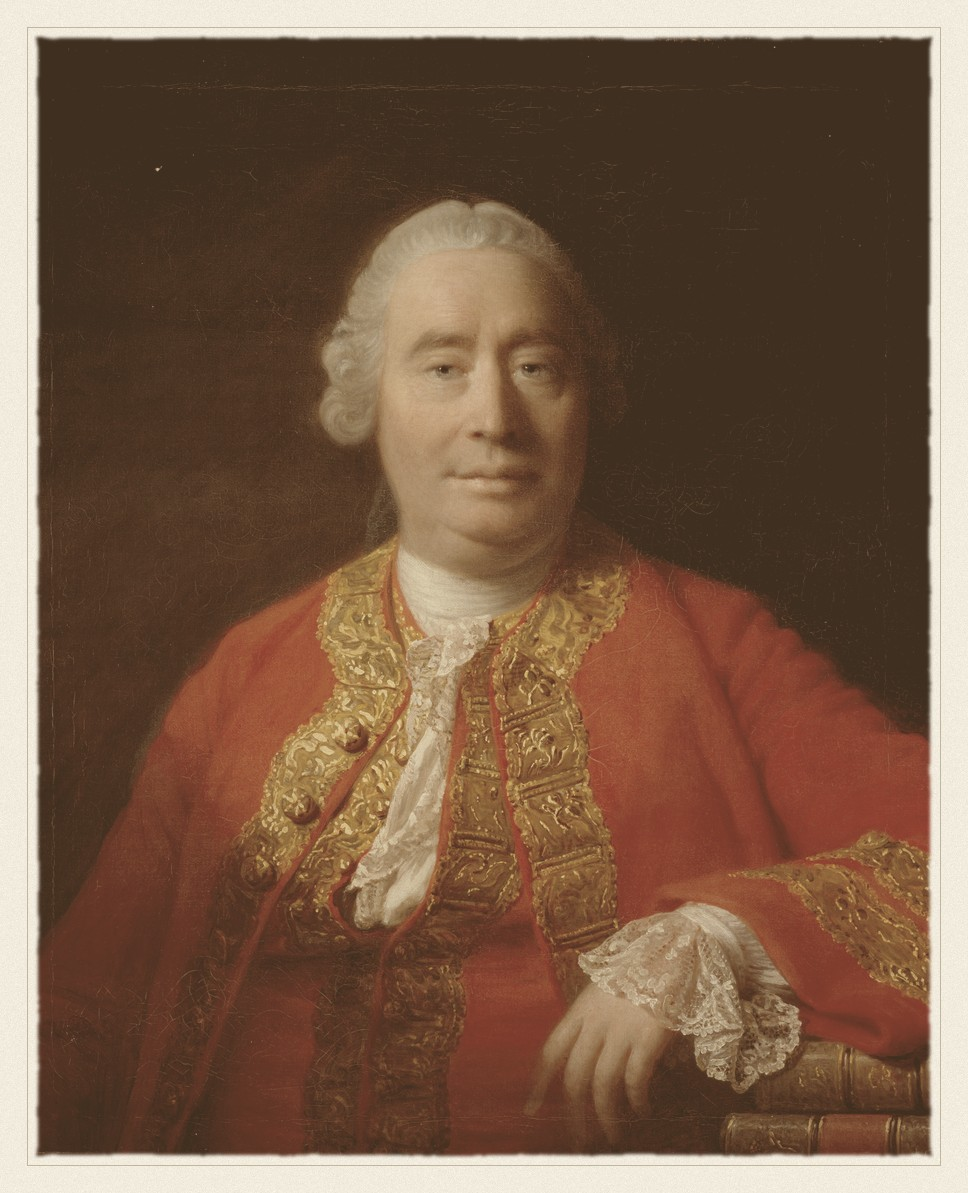
\includegraphics[keepaspectratio]{images/session-10-hume.jpg}}

\textbf{David Hume} · \textbf{1711--1776}

Asked what entitles us to say one thing causes another, and did not find
a satisfying answer. Neither has anyone since.

{Allan Ramsay, 1766. Public domain, via Wikimedia Commons.}

\end{qmibplate}

\begin{qmibarchive}

\textbf{From the archive · Hume, 1739}

David Hume asked what we actually observe when we say one thing causes
another, and answered: contiguity, succession, and constant conjunction.
The billiard ball moves; another moves after it; this has always
happened. What we never observe is the \emph{necessary connection} ---
the thing that would make the second event have to follow.

His second formulation is the one that founded modern causal inference,
though it took two centuries to be taken up. A cause, he wrote, is an
object followed by another, \emph{and where, if the first object had not
been, the second never had existed}. That subordinate clause is a
counterfactual: a statement about a world that did not happen. It cannot
be observed, in principle, for the same reason a road not taken has no
destination.

Hume treated this as a sceptical problem about knowledge. Modern
statistics treats it as a \emph{missing data} problem, which turns out
to be the more productive framing --- because missing data can sometimes
be recovered, under assumptions you can state, defend and occasionally
test.

\end{qmibarchive}

\section{Potential outcomes}\label{potential-outcomes}

The framework that formalises Hume's clause is due to Neyman and, in its
modern form, to Rubin (\citeproc{ref-rubin1974}{Donald B. Rubin 1974}).
For each unit \(i\) define two quantities:

\[
Y_i(1) = \text{the outcome if unit } i \text{ is treated},
\qquad
Y_i(0) = \text{the outcome if it is not}.
\]

Both are properties of the unit, defined whether or not the treatment
happens. The causal effect \emph{for that unit} is the difference

\[
\tau_i \;=\; Y_i(1) - Y_i(0),
\]

and it is exactly what Hume said we cannot observe: whichever treatment
the unit receives, the other potential outcome is missing, permanently
and by construction. This is the \textbf{fundamental problem of causal
inference} (\citeproc{ref-holland1986}{Holland 1986}), and it means that
no individual causal effect is ever identified. What we can hope for is
an \emph{average}.

\begin{qmibdefinition}

{\textbf{ATE}} --- average treatment effect,
\(\operatorname{E}[Y(1) - Y(0)]\) over the whole population. What would
happen if everyone were treated versus no one.

\end{qmibdefinition}

\begin{qmibdefinition}

{\textbf{ATT}} --- average treatment effect on the treated,
\(\operatorname{E}[Y(1) - Y(0) \mid T = 1]\). What the treatment did for
those who actually received it. Usually the policy-relevant quantity,
and usually not equal to the ATE.

\end{qmibdefinition}

Now the arithmetic that explains why naive comparisons fail. What you
can compute from data is the difference in observed means. Add and
subtract the same term:

\[
\underbrace{\operatorname{E}[Y \mid T{=}1] - \operatorname{E}[Y \mid T{=}0]}_{\text{what you can compute}}
=
\underbrace{\operatorname{E}[Y(1) - Y(0) \mid T{=}1]}_{\text{ATT}}
+
\underbrace{\operatorname{E}[Y(0) \mid T{=}1] - \operatorname{E}[Y(0) \mid T{=}0]}_{\text{selection bias}} .
\]

The second term is the difference between the treated and untreated
groups \emph{in the absence of treatment}. If countries that adopt a
policy would have differed from those that did not even without it, the
observed difference is the effect plus that gap, and nothing in the data
separates them.

\section{Randomisation, and what it
buys}\label{randomisation-and-what-it-buys}

Randomised assignment sets the selection term to zero, and it is worth
being precise about why. If treatment is assigned by a coin flip, then
\(T\) is independent of everything about the unit --- including \(Y(0)\)
and \(Y(1)\) --- so
\(\operatorname{E}[Y(0) \mid T{=}1] = \operatorname{E}[Y(0) \mid T{=}0]\)
and the bias term vanishes.

Note what randomisation does \emph{not} do. It does not make the groups
identical; in any finite sample they will differ, sometimes
substantially. It makes them differ \emph{in a way unrelated to the
outcome}, so the difference is noise rather than bias --- and noise is
what standard errors are for. It also balances variables nobody measured
or thought of, which is the property no observational method can
replicate.

When randomisation is unavailable, and in international business it
usually is --- countries are not randomly assigned national strategies
--- the alternative is to assume something strong enough to recover the
same result.

\begin{qmibdefinition}

{\textbf{Conditional independence}} (unconfoundedness, ignorability) ---
given a set of covariates \(X\), treatment is as good as random:
\(\{Y(0), Y(1)\} \perp T \mid X\). Every determinant of both treatment
and outcome is in \(X\). \textbf{This assumption is not testable},
because it concerns the missing potential outcome.

\end{qmibdefinition}

\begin{qmibdefinition}

{\textbf{Overlap}} (common support) --- for every value of \(X\), the
probability of treatment is strictly between 0 and 1. If some countries
would never adopt under any circumstances, there is no comparison to be
made for them, and an estimate that includes them is extrapolating
rather than comparing. Unlike conditional independence, overlap
\textbf{is} checkable.

\end{qmibdefinition}

\section{A treatment with a known
answer}\label{a-treatment-with-a-known-answer}

Everything above is standard and abstract. What follows is not available
in real work: an evaluation where the true effect is known, so each
method can be marked rather than argued about.

The course fixture contains a national AI strategy, adopted by some
countries in 2021, 2022 or 2023 and never by others. The generator that
built it did three things deliberately. It assigned treatment as a
function of two baseline country characteristics --- development and
institutional capacity --- so the data are \emph{confounded by
construction}. It set the true effect at \textbf{+2.4 percentage points}
on AI use. And it kept the infrastructure indicators free of any
treatment effect, so they are legitimate pre-treatment controls, while
the adoption indicators are downstream of treatment and are not.

\phantomsection\label{check-setup}
\begin{Shaded}
\begin{Highlighting}[]
\ImportTok{import}\NormalTok{ sys, warnings}
\NormalTok{sys.path.insert(}\DecValTok{0}\NormalTok{, }\StringTok{"../slides"}\NormalTok{)}\OperatorTok{;}\NormalTok{ sys.path.insert(}\DecValTok{0}\NormalTok{, }\StringTok{".."}\NormalTok{)}
\NormalTok{warnings.filterwarnings(}\StringTok{"ignore"}\NormalTok{)}
\ImportTok{from}\NormalTok{ plotstyle }\ImportTok{import}\NormalTok{ setup, CL}
\NormalTok{plt }\OperatorTok{=}\NormalTok{ setup()}

\ImportTok{import}\NormalTok{ numpy }\ImportTok{as}\NormalTok{ np, pandas }\ImportTok{as}\NormalTok{ pd, statsmodels.api }\ImportTok{as}\NormalTok{ sm, qmib}

\NormalTok{Y, T }\OperatorTok{=} \StringTok{"ai\_use\_any"}\NormalTok{, }\StringTok{"has\_ai\_strategy"}
\NormalTok{PRE }\OperatorTok{=}\NormalTok{ [}\StringTok{"cloud\_use"}\NormalTok{, }\StringTok{"ict\_specialists"}\NormalTok{, }\StringTok{"digital\_intensity"}\NormalTok{]}
\NormalTok{TRUE\_EFFECT }\OperatorTok{=} \FloatTok{2.4}          \CommentTok{\# from scripts/build\_spine/make\_fixtures.py}

\NormalTok{panel }\OperatorTok{=}\NormalTok{ qmib.load(}\StringTok{"angle\_c\_country"}\NormalTok{).dropna(}
\NormalTok{    subset}\OperatorTok{=}\NormalTok{[Y, T, }\StringTok{"ai\_use\_ml"}\NormalTok{] }\OperatorTok{+}\NormalTok{ PRE).copy()}

\BuiltInTok{print}\NormalTok{(}\SpecialStringTok{f"country{-}years: }\SpecialCharTok{\{}\BuiltInTok{len}\NormalTok{(panel)}\SpecialCharTok{\}}\SpecialStringTok{   treated: }\SpecialCharTok{\{}\BuiltInTok{int}\NormalTok{(panel[T].}\BuiltInTok{sum}\NormalTok{())}\SpecialCharTok{\}}\SpecialStringTok{   "}
      \SpecialStringTok{f"years }\SpecialCharTok{\{}\NormalTok{panel}\SpecialCharTok{.}\NormalTok{time}\SpecialCharTok{.}\BuiltInTok{min}\NormalTok{()}\SpecialCharTok{\}}\SpecialStringTok{–}\SpecialCharTok{\{}\NormalTok{panel}\SpecialCharTok{.}\NormalTok{time}\SpecialCharTok{.}\BuiltInTok{max}\NormalTok{()}\SpecialCharTok{\}}\SpecialStringTok{"}\NormalTok{)}
\BuiltInTok{print}\NormalTok{(}\SpecialStringTok{f"}\CharTok{\textbackslash{}n}\SpecialStringTok{adopting countries differ before treatment — standardised differences:"}\NormalTok{)}
\ControlFlowTok{for}\NormalTok{ c }\KeywordTok{in}\NormalTok{ PRE:}
\NormalTok{    a, b }\OperatorTok{=}\NormalTok{ panel.loc[panel[T] }\OperatorTok{==} \DecValTok{1}\NormalTok{, c], panel.loc[panel[T] }\OperatorTok{==} \DecValTok{0}\NormalTok{, c]}
\NormalTok{    smd }\OperatorTok{=}\NormalTok{ (a.mean() }\OperatorTok{{-}}\NormalTok{ b.mean()) }\OperatorTok{/}\NormalTok{ np.sqrt((a.var(ddof}\OperatorTok{=}\DecValTok{1}\NormalTok{) }\OperatorTok{+}\NormalTok{ b.var(ddof}\OperatorTok{=}\DecValTok{1}\NormalTok{)) }\OperatorTok{/} \DecValTok{2}\NormalTok{)}
    \BuiltInTok{print}\NormalTok{(}\SpecialStringTok{f"   }\SpecialCharTok{\{}\NormalTok{c}\SpecialCharTok{:22\}\{}\NormalTok{smd}\SpecialCharTok{:+7.3f\}}\SpecialStringTok{"}\NormalTok{)}
\BuiltInTok{print}\NormalTok{(}\StringTok{"}\CharTok{\textbackslash{}n}\StringTok{A standardised difference near 1 is a large imbalance. These countries"}\NormalTok{)}
\BuiltInTok{print}\NormalTok{(}\StringTok{"were already more digital before any strategy existed — which is exactly"}\NormalTok{)}
\BuiltInTok{print}\NormalTok{(}\StringTok{"the selection term in the decomposition above."}\NormalTok{)}
\end{Highlighting}
\end{Shaded}

\begin{verbatim}
country-years: 91   treated: 49   years 2021–2024

adopting countries differ before treatment — standardised differences:
   cloud_use              +0.972
   ict_specialists        +0.998
   digital_intensity      +1.138

A standardised difference near 1 is a large imbalance. These countries
were already more digital before any strategy existed — which is exactly
the selection term in the decomposition above.
\end{verbatim}

\section{Four estimates, one truth}\label{four-estimates-one-truth}

\phantomsection\label{check-estimators}
\begin{Shaded}
\begin{Highlighting}[]
\KeywordTok{def}\NormalTok{ report(label, estimate, se}\OperatorTok{=}\VariableTok{None}\NormalTok{):}
\NormalTok{    tail }\OperatorTok{=} \SpecialStringTok{f"   (SE }\SpecialCharTok{\{}\NormalTok{se}\SpecialCharTok{:.3f\}}\SpecialStringTok{)"} \ControlFlowTok{if}\NormalTok{ se }\KeywordTok{is} \KeywordTok{not} \VariableTok{None} \ControlFlowTok{else} \StringTok{""}
    \BuiltInTok{print}\NormalTok{(}\SpecialStringTok{f"}\SpecialCharTok{\{}\NormalTok{label}\SpecialCharTok{:38\}\{}\NormalTok{estimate}\SpecialCharTok{:+8.3f\}\{}\NormalTok{estimate }\OperatorTok{{-}}\NormalTok{ TRUE\_EFFECT}\SpecialCharTok{:+10.3f\}\{}\NormalTok{tail}\SpecialCharTok{\}}\SpecialStringTok{"}\NormalTok{)}

\BuiltInTok{print}\NormalTok{(}\SpecialStringTok{f"}\SpecialCharTok{\{}\StringTok{\textquotesingle{}method\textquotesingle{}}\SpecialCharTok{:38\}\{}\StringTok{\textquotesingle{}estimate\textquotesingle{}}\SpecialCharTok{:\textgreater{}8\}\{}\StringTok{\textquotesingle{}bias\textquotesingle{}}\SpecialCharTok{:\textgreater{}10\}}\SpecialStringTok{"}\NormalTok{)}
\NormalTok{report(}\StringTok{"the truth (from the generator)"}\NormalTok{, TRUE\_EFFECT)}

\NormalTok{naive }\OperatorTok{=}\NormalTok{ panel.loc[panel[T] }\OperatorTok{==} \DecValTok{1}\NormalTok{, Y].mean() }\OperatorTok{{-}}\NormalTok{ panel.loc[panel[T] }\OperatorTok{==} \DecValTok{0}\NormalTok{, Y].mean()}
\NormalTok{report(}\StringTok{"naive difference in means"}\NormalTok{, naive)}

\NormalTok{adj }\OperatorTok{=}\NormalTok{ sm.OLS(panel[Y], sm.add\_constant(panel[[T] }\OperatorTok{+}\NormalTok{ PRE])).fit(}
\NormalTok{    cov\_type}\OperatorTok{=}\StringTok{"cluster"}\NormalTok{, cov\_kwds}\OperatorTok{=}\NormalTok{\{}\StringTok{"groups"}\NormalTok{: panel[}\StringTok{"geo"}\NormalTok{]\})}
\NormalTok{report(}\StringTok{"regression on pre{-}treatment controls"}\NormalTok{, adj.params[T], adj.bse[T])}

\CommentTok{\# 1:1 nearest{-}neighbour matching on the estimated propensity score}
\NormalTok{ps }\OperatorTok{=}\NormalTok{ sm.Logit(panel[T], sm.add\_constant(panel[PRE])).fit(disp}\OperatorTok{=}\DecValTok{0}\NormalTok{).predict()}
\NormalTok{panel }\OperatorTok{=}\NormalTok{ panel.assign(ps}\OperatorTok{=}\NormalTok{ps)}
\NormalTok{tr, co }\OperatorTok{=}\NormalTok{ panel[panel[T] }\OperatorTok{==} \DecValTok{1}\NormalTok{], panel[panel[T] }\OperatorTok{==} \DecValTok{0}\NormalTok{]}
\NormalTok{nn }\OperatorTok{=}\NormalTok{ np.}\BuiltInTok{abs}\NormalTok{(tr[}\StringTok{"ps"}\NormalTok{].values[:, }\VariableTok{None}\NormalTok{] }\OperatorTok{{-}}\NormalTok{ co[}\StringTok{"ps"}\NormalTok{].values[}\VariableTok{None}\NormalTok{, :]).argmin(axis}\OperatorTok{=}\DecValTok{1}\NormalTok{)}
\NormalTok{matched }\OperatorTok{=}\NormalTok{ co.iloc[nn]}
\NormalTok{report(}\StringTok{"propensity{-}score matching (ATT)"}\NormalTok{,}
\NormalTok{       (tr[Y].values }\OperatorTok{{-}}\NormalTok{ matched[Y].values).mean())}

\NormalTok{bad }\OperatorTok{=}\NormalTok{ sm.OLS(panel[Y], sm.add\_constant(panel[[T] }\OperatorTok{+}\NormalTok{ PRE }\OperatorTok{+}\NormalTok{ [}\StringTok{"ai\_use\_ml"}\NormalTok{]])).fit(}
\NormalTok{    cov\_type}\OperatorTok{=}\StringTok{"cluster"}\NormalTok{, cov\_kwds}\OperatorTok{=}\NormalTok{\{}\StringTok{"groups"}\NormalTok{: panel[}\StringTok{"geo"}\NormalTok{]\})}
\NormalTok{report(}\StringTok{"+ a post{-}treatment control"}\NormalTok{, bad.params[T], bad.bse[T])}
\end{Highlighting}
\end{Shaded}

\begin{verbatim}
method                                estimate      bias
the truth (from the generator)          +2.400    +0.000
naive difference in means               +6.069    +3.669
regression on pre-treatment controls    +3.101    +0.701   (SE 0.365)
propensity-score matching (ATT)         +2.678    +0.278
+ a post-treatment control              +2.153    -0.247   (SE 0.433)
\end{verbatim}

The naive comparison overstates the effect by more than 150\%. That is
the selection term made visible: adopting countries were already more
digital, and the difference in outcomes is mostly the difference in
countries.

Adjusting for the pre-treatment indicators removes most of it but not
all, leaving about +0.7 percentage points of bias. The reason is worth
stating, because it is the normal situation and not a defect of this
example: the observed indicators are \emph{noisy proxies} for the latent
characteristics that actually drove adoption. Conditioning on a proxy
removes the part of the confounding it captures and leaves the rest.

Matching does best. And the last line is the interesting one.

\section{The control that improves the number and ruins the
estimate}\label{the-control-that-improves-the-number-and-ruins-the-estimate}

Adding a post-treatment variable moved the estimate closer to the truth.
It is still wrong to do it, and understanding why is more valuable than
the number.

\texttt{ai\_use\_ml} is a \emph{consequence} of the strategy, not a
cause of it. Conditioning on it blocks part of the causal path from
treatment to outcome, so the coefficient on treatment no longer measures
the total effect --- it measures whatever is left after the mediated
portion has been removed. That it lands near the truth here is a
coincidence: the downward bias from blocking the path happened to offset
the residual upward bias from imperfect proxies.

\begin{qmibwarn}

\textbf{``Closer to the right answer'' is not the same as ``the right
method.''} In real work the truth is unknown, so the only evidence
available is whether the procedure is justified. A procedure that is
wrong for a reason you can state will be wrong by an unknown amount in
the next dataset, and no diagnostic will announce it.

\end{qmibwarn}

This is the general problem of bad controls. The instinct that adding
covariates is prudent is wrong in two specific cases: a
\textbf{mediator}, which sits on the causal path and whose inclusion
removes part of the effect you are estimating; and a \textbf{collider},
a common consequence of treatment and outcome, whose inclusion
\emph{creates} an association that does not exist
(\citeproc{ref-elwert2014}{Elwert and Winship 2014}). Deciding what
belongs in the regression is a claim about causal structure, not a
statistical choice, and Cinelli, Forney, and Pearl
(\citeproc{ref-cinelli2022}{2022}) is the short guide worth keeping
beside the keyboard.

\section{Balance is the diagnostic, not
fit}\label{balance-is-the-diagnostic-not-fit}

The most important shift in this chapter is what counts as evidence that
the estimate is any good. Chapter 3 judged a model by its residuals. A
matching estimator is judged by whether the groups it compares are
actually comparable.

\begin{Shaded}
\begin{Highlighting}[]
\KeywordTok{def}\NormalTok{ smd(a, b):}
    \ControlFlowTok{return}\NormalTok{ (a.mean() }\OperatorTok{{-}}\NormalTok{ b.mean()) }\OperatorTok{/}\NormalTok{ np.sqrt((a.var(ddof}\OperatorTok{=}\DecValTok{1}\NormalTok{) }\OperatorTok{+}\NormalTok{ b.var(ddof}\OperatorTok{=}\DecValTok{1}\NormalTok{)) }\OperatorTok{/} \DecValTok{2}\NormalTok{)}

\NormalTok{names }\OperatorTok{=}\NormalTok{ PRE }\OperatorTok{+}\NormalTok{ [}\StringTok{"ps"}\NormalTok{]}
\NormalTok{before }\OperatorTok{=}\NormalTok{ [smd(tr[c], co[c]) }\ControlFlowTok{for}\NormalTok{ c }\KeywordTok{in}\NormalTok{ names]}
\NormalTok{after }\OperatorTok{=}\NormalTok{ [smd(tr[c], matched[c]) }\ControlFlowTok{for}\NormalTok{ c }\KeywordTok{in}\NormalTok{ names]}

\NormalTok{fig, ax }\OperatorTok{=}\NormalTok{ plt.subplots(figsize}\OperatorTok{=}\NormalTok{(}\FloatTok{7.0}\NormalTok{, }\FloatTok{3.4}\NormalTok{))}
\NormalTok{yy }\OperatorTok{=}\NormalTok{ np.arange(}\BuiltInTok{len}\NormalTok{(names))}
\NormalTok{ax.axvline(}\DecValTok{0}\NormalTok{, color}\OperatorTok{=}\NormalTok{CL.line, lw}\OperatorTok{=}\DecValTok{1}\NormalTok{)}
\ControlFlowTok{for}\NormalTok{ x }\KeywordTok{in}\NormalTok{ (}\OperatorTok{{-}}\FloatTok{0.1}\NormalTok{, }\FloatTok{0.1}\NormalTok{):}
\NormalTok{    ax.axvline(x, color}\OperatorTok{=}\NormalTok{CL.muted, lw}\OperatorTok{=}\DecValTok{1}\NormalTok{, ls}\OperatorTok{=}\StringTok{"{-}{-}"}\NormalTok{)}
\NormalTok{ax.scatter(before, yy, s}\OperatorTok{=}\DecValTok{58}\NormalTok{, color}\OperatorTok{=}\NormalTok{CL.warn, label}\OperatorTok{=}\StringTok{"before matching"}\NormalTok{, zorder}\OperatorTok{=}\DecValTok{3}\NormalTok{)}
\NormalTok{ax.scatter(after, yy, s}\OperatorTok{=}\DecValTok{58}\NormalTok{, color}\OperatorTok{=}\NormalTok{CL.good, label}\OperatorTok{=}\StringTok{"after matching"}\NormalTok{, zorder}\OperatorTok{=}\DecValTok{3}\NormalTok{)}
\ControlFlowTok{for}\NormalTok{ i, (b\_, a\_) }\KeywordTok{in} \BuiltInTok{enumerate}\NormalTok{(}\BuiltInTok{zip}\NormalTok{(before, after)):}
\NormalTok{    ax.plot([b\_, a\_], [i, i], color}\OperatorTok{=}\NormalTok{CL.muted, lw}\OperatorTok{=}\DecValTok{1}\NormalTok{, alpha}\OperatorTok{=}\FloatTok{0.5}\NormalTok{, zorder}\OperatorTok{=}\DecValTok{2}\NormalTok{)}
\NormalTok{ax.set\_yticks(yy)}\OperatorTok{;}\NormalTok{ ax.set\_yticklabels(names)}
\NormalTok{ax.set\_xlabel(}\StringTok{"standardised mean difference"}\NormalTok{)}
\NormalTok{ax.legend(frameon}\OperatorTok{=}\VariableTok{False}\NormalTok{, fontsize}\OperatorTok{=}\FloatTok{8.5}\NormalTok{, loc}\OperatorTok{=}\StringTok{"lower right"}\NormalTok{)}
\NormalTok{fig.tight\_layout()}

\BuiltInTok{print}\NormalTok{(}\SpecialStringTok{f"}\SpecialCharTok{\{}\StringTok{\textquotesingle{}covariate\textquotesingle{}}\SpecialCharTok{:22\}\{}\StringTok{\textquotesingle{}before\textquotesingle{}}\SpecialCharTok{:\textgreater{}9\}\{}\StringTok{\textquotesingle{}after\textquotesingle{}}\SpecialCharTok{:\textgreater{}9\}}\SpecialStringTok{"}\NormalTok{)}
\ControlFlowTok{for}\NormalTok{ n, b\_, a\_ }\KeywordTok{in} \BuiltInTok{zip}\NormalTok{(names, before, after):}
    \BuiltInTok{print}\NormalTok{(}\SpecialStringTok{f"}\SpecialCharTok{\{}\NormalTok{n}\SpecialCharTok{:22\}\{}\NormalTok{b\_}\SpecialCharTok{:+9.3f\}\{}\NormalTok{a\_}\SpecialCharTok{:+9.3f\}}\SpecialStringTok{"}\NormalTok{)}
\BuiltInTok{print}\NormalTok{(}\SpecialStringTok{f"}\CharTok{\textbackslash{}n}\SpecialStringTok{overlap in the propensity score:"}\NormalTok{)}
\BuiltInTok{print}\NormalTok{(}\SpecialStringTok{f"   treated  }\SpecialCharTok{\{}\NormalTok{tr[}\StringTok{\textquotesingle{}ps\textquotesingle{}}\NormalTok{]}\SpecialCharTok{.}\BuiltInTok{min}\NormalTok{()}\SpecialCharTok{:.3f\}}\SpecialStringTok{ – }\SpecialCharTok{\{}\NormalTok{tr[}\StringTok{\textquotesingle{}ps\textquotesingle{}}\NormalTok{]}\SpecialCharTok{.}\BuiltInTok{max}\NormalTok{()}\SpecialCharTok{:.3f\}}\SpecialStringTok{"}\NormalTok{)}
\BuiltInTok{print}\NormalTok{(}\SpecialStringTok{f"   control  }\SpecialCharTok{\{}\NormalTok{co[}\StringTok{\textquotesingle{}ps\textquotesingle{}}\NormalTok{]}\SpecialCharTok{.}\BuiltInTok{min}\NormalTok{()}\SpecialCharTok{:.3f\}}\SpecialStringTok{ – }\SpecialCharTok{\{}\NormalTok{co[}\StringTok{\textquotesingle{}ps\textquotesingle{}}\NormalTok{]}\SpecialCharTok{.}\BuiltInTok{max}\NormalTok{()}\SpecialCharTok{:.3f\}}\SpecialStringTok{"}\NormalTok{)}
\end{Highlighting}
\end{Shaded}

\begin{verbatim}
covariate                before    after
cloud_use                +0.972   +0.033
ict_specialists          +0.998   -0.061
digital_intensity        +1.138   +0.037
ps                       +1.200   +0.019

overlap in the propensity score:
   treated  0.245 – 0.970
   control  0.051 – 0.931
\end{verbatim}

\begin{figure}[htbp]

\centering{

\pandocbounded{
\includegraphics[keepaspectratio]{session-10_files/figure-pdf/fig-balance-output-2.png}}

}

\caption{\label{fig-balance}Covariate balance before and after matching.
Each point is the standardised difference between treated and control
groups; the dashed lines mark the conventional 0.1 threshold. Before
matching every covariate is imbalanced by around one standard deviation;
after, all lie inside the threshold.}

\end{figure}%

The convention is that a standardised difference below 0.1 is acceptable
balance. Before matching, every covariate is out by around a full
standard deviation; after, all four sit inside the threshold.
\textbf{That is the result to report} --- not the R² of the propensity
model, which is irrelevant, and not its coefficients, which are a means
and not an end.

The overlap figures matter too. The treated propensity scores span a
range the controls also cover, so every treated unit has a plausible
comparison. Had the treated run from 0.9 to 1.0 while controls stopped
at 0.4, there would be no comparable units and the honest response is to
restrict the sample and say the estimate applies only to the region
where comparison was possible.

One caution about the method itself. Propensity-score matching is the
most popular approach here and not the best one: matching on a scalar
score discards information and can \emph{increase} imbalance as the
caliper tightens, a pathology documented at length by King and Nielsen
(\citeproc{ref-king2019}{2019}). Matching directly on the covariates, or
weighting rather than matching, generally does better. The score remains
a good diagnostic for overlap even where it is a poor matching device.

\section{What none of this fixes}\label{what-none-of-this-fixes}

The estimate above came within 0.3 percentage points of the truth. It
would be a mistake to conclude that matching solved the problem, because
the assumption that licensed it was true \emph{by construction} --- the
generator used exactly those covariates to assign treatment, so
conditioning on them is sufficient.

In real work you never know that. Conditional independence is
untestable, and the honest response is to ask how wrong it could be.
Sensitivity analysis asks: how strong would an unobserved confounder
have to be --- how strongly associated with both treatment and outcome
--- to overturn the conclusion? If the answer is ``about as strong as
the covariates already controlled for'', the finding is fragile. If it
is ``stronger than any known determinant'', it is robust. Either way the
reader learns something a point estimate does not tell them.

The deeper limitation is that matching and regression adjustment are the
\emph{same assumption} in different clothing. Both require that
conditioning on observed covariates suffices. Neither creates
identification; they only implement it. When the assumption fails, both
fail, and they fail in the same direction.

Chapter 11 takes the other route: rather than assuming the confounders
are all observed, it uses the structure of \emph{when} treatment arrived
--- the staggered adoption in this very dataset --- to difference the
unobserved ones away.

\section{A short review of the
literature}\label{a-short-review-of-the-literature-8}

\begin{qmiblit}

The potential-outcomes notation is Donald B. Rubin
(\citeproc{ref-rubin1974}{1974}), though the idea traces to Neyman's
1923 work on agricultural experiments. Holland
(\citeproc{ref-holland1986}{1986}) named the fundamental problem and
drew the boundary the discipline still uses --- ``no causation without
manipulation'' --- which remains contested and clarifying.

Rosenbaum and Rubin (\citeproc{ref-rosenbaum1983}{1983}) proved the
result that made observational adjustment tractable: if treatment is
unconfounded given a covariate vector, it is unconfounded given the
scalar propensity score alone, so a many-dimensional matching problem
collapses to one dimension. Imbens (\citeproc{ref-imbens2004}{2004})
surveys the estimators that followed and Stuart
(\citeproc{ref-stuart2010}{2010}) is the practical review, covering
matching, weighting and the diagnostics that should accompany them.

The corrective literature is as important as the constructive one. King
and Nielsen (\citeproc{ref-king2019}{2019}) argues that propensity-score
matching specifically --- as opposed to matching in general --- often
increases imbalance and should be replaced by methods that match on
covariates directly. Elwert and Winship
(\citeproc{ref-elwert2014}{2014}) sets out endogenous selection bias,
the family of errors created by conditioning on colliders, and Cinelli,
Forney, and Pearl (\citeproc{ref-cinelli2022}{2022}) gives the compact
treatment of which controls help and which do damage.

\end{qmiblit}

\section{What to report}\label{what-to-report-8}

\begin{enumerate}
\def\labelenumi{\arabic{enumi}.}
\tightlist
\item
  \textbf{The estimand, named.} ATE or ATT --- they answer different
  questions and matching usually estimates the second.
\item
  \textbf{The identifying assumption, in words.} Which variables are
  claimed to close every path from treatment to outcome, and why that
  list is complete. This is an argument, not a table.
\item
  \textbf{Balance before and after}, for every covariate, with
  standardised differences. Not the propensity model's coefficients or
  its fit.
\item
  \textbf{Overlap}, with the range of the score in both groups, and what
  you did about units outside common support.
\item
  \textbf{The naive estimate alongside the adjusted one.} The distance
  between them is the size of the selection problem, and hiding it hides
  the reason for the analysis.
\item
  \textbf{A sensitivity analysis.} How strong an unobserved confounder
  would need to be to overturn the result.
\item
  \textbf{That every control is pre-treatment}, and that you know it. If
  a covariate is measured after treatment, say why it is not a mediator
  or a collider --- and if you cannot, drop it, even when it improves
  the number.
\end{enumerate}

\bookmarksetup{startatroot}

\chapter{Causal Inference II:
Difference-in-Differences}\label{causal-inference-ii-difference-in-differences}

\section{What would have happened
otherwise}\label{what-would-have-happened-otherwise}

Chapter 10 recovered a causal effect by assuming that the variables
driving treatment were all observed, and then conditioning on them. That
assumption is untestable and, in most settings, false --- countries do
not adopt policies for reasons that are fully captured by three
indicators.

This chapter takes the opposite route. Rather than measuring the
confounders, it uses \emph{timing} to remove them: if a country's
unobserved characteristics are stable over a short window, then
comparing that country to itself before and after differences them away.
The remaining problem --- that things change over time for everyone ---
is handled by a second comparison, against units that did not adopt.

Two differences, hence the name.

\begin{qmibplate}

\pandocbounded{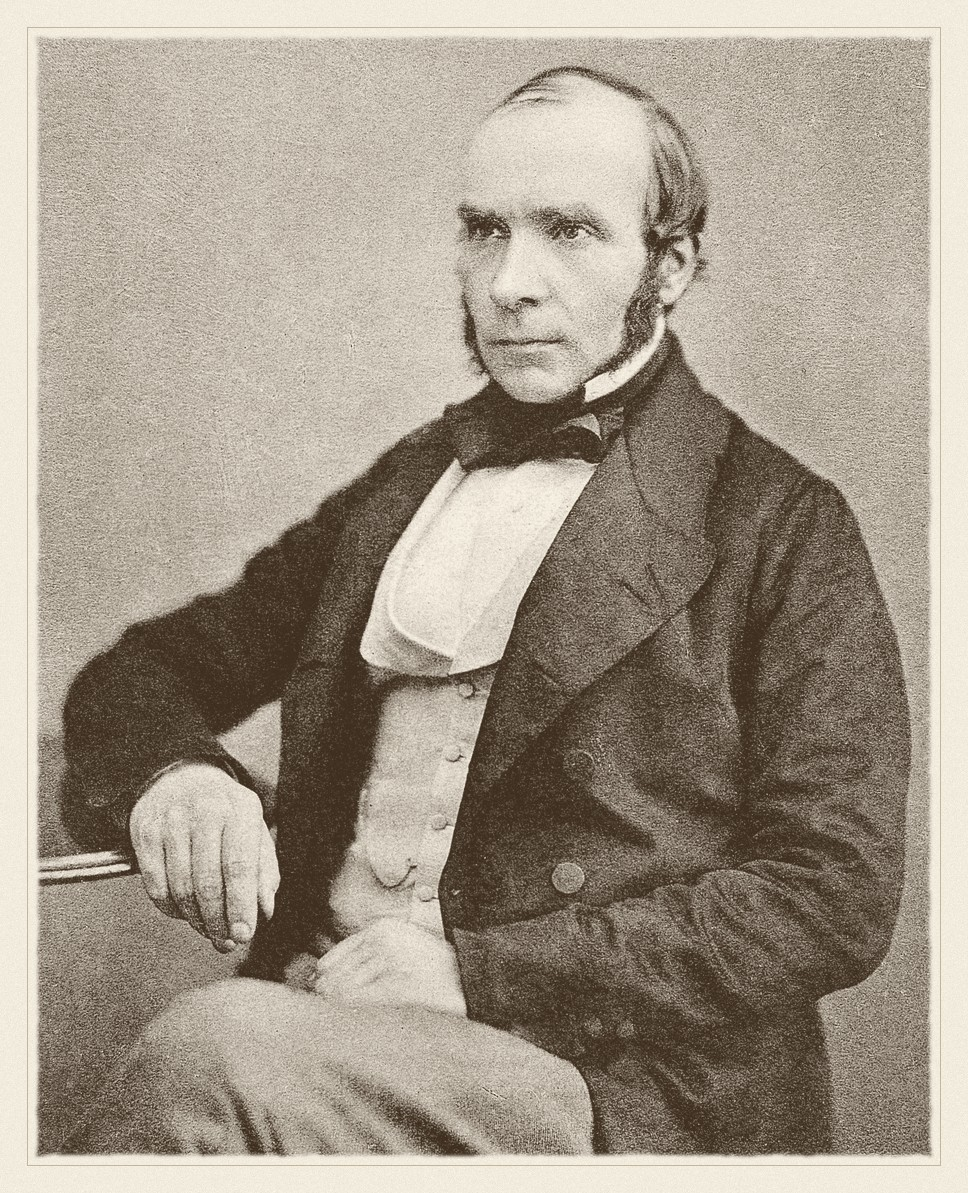
\includegraphics[keepaspectratio]{images/session-11-snow.jpg}}

\textbf{John Snow} · \textbf{1813--1858}

Mapped cholera deaths in 1854 and read a natural experiment off the
water supply --- before the statistics existed to justify it.

{unknown, Autotype 1856, published in 1887. Public domain, via Wikimedia
Commons.}

\end{qmibplate}

\begin{qmibarchive}

\textbf{From the archive · Snow, 1855}

John Snow is remembered for the Broad Street pump, which is the wrong
story. The map of cholera deaths clustered around one pump was
suggestive, but a sceptic could reply that the people near the pump were
poorer, more crowded, and different in a dozen ways from those further
off --- the selection problem of chapter 10, in 1854.

His second study answered that objection, and it is the one that matters
here. Two companies supplied water to overlapping districts of south
London, their pipes running down the same streets so that neighbouring
houses drew from different sources. In 1852 one of them, Lambeth, moved
its intake upstream of the sewage outflows; the other, Southwark and
Vauxhall, did not. Snow could therefore compare cholera mortality in
households that differed in water supply but not, in any systematic way,
in anything else --- and compare the change over time between the two.

He called it ``an experiment on the grandest scale'', and was explicit
that its force came from the \emph{assignment}: no one chose their
supplier, the pipes had been laid years earlier for commercial reasons
unrelated to the disease. That is the argument every
difference-in-differences paper is still making. Snow made it before the
germ theory of disease existed --- he had no mechanism, only a design.

\end{qmibarchive}

\section{The two differences}\label{the-two-differences}

Let \(\bar Y_{g,t}\) be the average outcome for group \(g\) in period
\(t\), with \(g \in \{\text{treated}, \text{control}\}\) and
\(t \in \{\text{pre}, \text{post}\}\). The estimator is

\[
\widehat{\text{DiD}}
=
\underbrace{\big(\bar Y_{\text{tr,post}} - \bar Y_{\text{tr,pre}}\big)}_{\text{change among the treated}}
-
\underbrace{\big(\bar Y_{\text{co,post}} - \bar Y_{\text{co,pre}}\big)}_{\text{change among the controls}} .
\]

The first difference removes everything time-invariant about the treated
group, observed or not --- its wealth, its institutions, its geography.
The second estimates what would have happened anyway, and subtracting it
removes any shock common to both groups.

What licenses the subtraction is a single assumption, and it is worth
stating in its exact form because the loose version is misleading.

\begin{qmibdefinition}

{\textbf{Parallel trends}} --- in the absence of treatment, the average
outcome of the treated group would have followed the same
\emph{trajectory} as the control group. Formally, \[
\operatorname{E}[Y_{\text{tr,post}}(0) - Y_{\text{tr,pre}}(0)]
=
\operatorname{E}[Y_{\text{co,post}}(0) - Y_{\text{co,pre}}(0)] .
\] It is not an assumption that the groups are \emph{similar} --- they
may differ by any amount in level --- only that the gap between them
would have stayed constant.

\end{qmibdefinition}

The assumption concerns \(Y(0)\) for the treated group in the post
period, which is precisely the counterfactual that does not exist.
\textbf{Parallel trends is therefore untestable}, in the same way and
for the same reason as chapter 10's conditional independence. What can
be examined is whether the trends were parallel \emph{before} treatment,
which is evidence about plausibility rather than a test of the
assumption itself.

Note also that parallel trends is not invariant to how the outcome is
measured. If two groups have parallel trends in levels they generally do
not in logs, and vice versa, so the choice of scale is part of the
identifying assumption rather than a presentational detail.

\section{As a regression}\label{as-a-regression}

The two-by-two table is easier to work with as a regression, and the
regression form is one you have already met. With unit and period fixed
effects,

\[
Y_{it} \;=\; \alpha_i + \gamma_t + \delta \, D_{it} + \varepsilon_{it},
\]

where \(D_{it}\) is 1 when unit \(i\) is treated in period \(t\), the
coefficient \(\delta\) \emph{is} the difference-in-differences estimate.
That is chapter 6's two-way fixed effects specification with the
treatment indicator in place of a continuous regressor: the unit effects
absorb the first difference, the period effects the second.

The regression form buys three things --- covariates, more than two
periods and more than two groups, and standard errors. On the last,
chapter 3's finding returns with force: DiD data are panels, residuals
are serially correlated within unit, and treating the country-years as
independent understates the standard error badly. Clustering by unit is
the minimum, and the classic demonstration of what happens otherwise is
Bertrand, Duflo and Mullainathan's, cited in chapter 3.

\section{When treatment arrives at different
times}\label{when-treatment-arrives-at-different-times}

The clean two-by-two case has one treatment date. Real policies arrive
in different years for different units --- which is exactly what the
course fixture contains --- and for two decades the profession simply
put a treatment dummy into a two-way fixed effects regression and read
off the coefficient.

That turns out to be wrong in a way nobody noticed until recently. With
staggered timing, the TWFE estimate is a \emph{weighted average} of all
the two-by-two comparisons available in the data, and some of those
comparisons use already-treated units as controls for later-treated
ones. When effects vary over time --- when the policy's impact grows,
say --- those comparisons subtract a treatment effect rather than a
counterfactual trend, and the implied weights can be \textbf{negative}
(\citeproc{ref-dechaisemartin2020}{Chaisemartin and D'Haultfœuille
2020}; \citeproc{ref-goodmanbacon2021}{Goodman-Bacon 2021}). A weighted
average with negative weights can lie outside the range of the things
being averaged, so the estimate can have the wrong sign while every
underlying effect has the right one.

The remedy is to build the average yourself: estimate each cohort's
effect against clean controls --- units not yet treated, or never
treated --- and aggregate with weights you chose
(\citeproc{ref-callaway2021}{Callaway and Sant'Anna 2021};
\citeproc{ref-sun2021}{Sun and Abraham 2021}).

\section{The data, and what it will and will not
support}\label{the-data-and-what-it-will-and-will-not-support}

\phantomsection\label{check-timing}
\begin{Shaded}
\begin{Highlighting}[]
\ImportTok{import}\NormalTok{ sys, warnings}
\NormalTok{sys.path.insert(}\DecValTok{0}\NormalTok{, }\StringTok{"../slides"}\NormalTok{)}\OperatorTok{;}\NormalTok{ sys.path.insert(}\DecValTok{0}\NormalTok{, }\StringTok{".."}\NormalTok{)}
\NormalTok{warnings.filterwarnings(}\StringTok{"ignore"}\NormalTok{)}
\ImportTok{from}\NormalTok{ plotstyle }\ImportTok{import}\NormalTok{ setup, CL}
\NormalTok{plt }\OperatorTok{=}\NormalTok{ setup()}

\ImportTok{import}\NormalTok{ numpy }\ImportTok{as}\NormalTok{ np, pandas }\ImportTok{as}\NormalTok{ pd, statsmodels.api }\ImportTok{as}\NormalTok{ sm, qmib}

\NormalTok{Y, D }\OperatorTok{=} \StringTok{"ai\_use\_any"}\NormalTok{, }\StringTok{"has\_ai\_strategy"}
\NormalTok{TRUE\_EFFECT }\OperatorTok{=} \FloatTok{2.4}               \CommentTok{\# from scripts/build\_spine/make\_fixtures.py}

\NormalTok{wide }\OperatorTok{=}\NormalTok{ qmib.load(}\StringTok{"angle\_c\_country"}\NormalTok{)}

\CommentTok{\# Adoption year must come from the FULL treatment series, not from the rows where}
\CommentTok{\# the outcome happens to be observed. Two countries adopted in 2022 and have a}
\CommentTok{\# missing 2022 outcome; taking the first year they are *seen* treated would put}
\CommentTok{\# them in the 2023 cohort and silently misdate the policy.}
\NormalTok{adopted }\OperatorTok{=}\NormalTok{ wide[wide[D] }\OperatorTok{==} \DecValTok{1}\NormalTok{].groupby(}\StringTok{"geo"}\NormalTok{)[}\StringTok{"time"}\NormalTok{].}\BuiltInTok{min}\NormalTok{()}

\NormalTok{panel }\OperatorTok{=}\NormalTok{ wide[(wide[}\StringTok{"time"}\NormalTok{] }\OperatorTok{\textgreater{}=} \DecValTok{2021}\NormalTok{) }\OperatorTok{\&}\NormalTok{ wide[Y].notna()].copy()}
\NormalTok{panel[}\StringTok{"cohort"}\NormalTok{] }\OperatorTok{=}\NormalTok{ panel[}\StringTok{"geo"}\NormalTok{].}\BuiltInTok{map}\NormalTok{(adopted).fillna(}\DecValTok{9999}\NormalTok{).astype(}\BuiltInTok{int}\NormalTok{)}

\BuiltInTok{print}\NormalTok{(}\SpecialStringTok{f"country{-}years with the outcome observed: }\SpecialCharTok{\{}\BuiltInTok{len}\NormalTok{(panel)}\SpecialCharTok{\}}\SpecialStringTok{"}\NormalTok{)}
\BuiltInTok{print}\NormalTok{(}\SpecialStringTok{f"the outcome exists only from }\SpecialCharTok{\{}\BuiltInTok{int}\NormalTok{(panel.time.}\BuiltInTok{min}\NormalTok{())}\SpecialCharTok{\}}\SpecialStringTok{ — "}
      \SpecialStringTok{f"the AI module did not exist before it}\CharTok{\textbackslash{}n}\SpecialStringTok{"}\NormalTok{)}
\BuiltInTok{print}\NormalTok{(}\SpecialStringTok{f"}\SpecialCharTok{\{}\StringTok{\textquotesingle{}cohort\textquotesingle{}}\SpecialCharTok{:\textgreater{}10\}\{}\StringTok{\textquotesingle{}countries\textquotesingle{}}\SpecialCharTok{:\textgreater{}11\}}\SpecialStringTok{   pre{-}periods available"}\NormalTok{)}
\ControlFlowTok{for}\NormalTok{ c }\KeywordTok{in} \BuiltInTok{sorted}\NormalTok{(panel[}\StringTok{"cohort"}\NormalTok{].unique()):}
\NormalTok{    n }\OperatorTok{=}\NormalTok{ panel.loc[panel[}\StringTok{"cohort"}\NormalTok{] }\OperatorTok{==}\NormalTok{ c, }\StringTok{"geo"}\NormalTok{].nunique()}
    \ControlFlowTok{if}\NormalTok{ c }\OperatorTok{==} \DecValTok{9999}\NormalTok{:}
        \BuiltInTok{print}\NormalTok{(}\SpecialStringTok{f"}\SpecialCharTok{\{}\StringTok{\textquotesingle{}never\textquotesingle{}}\SpecialCharTok{:\textgreater{}10\}\{}\NormalTok{n}\SpecialCharTok{:\textgreater{}11\}}\SpecialStringTok{   —"}\NormalTok{)}
    \ControlFlowTok{else}\NormalTok{:}
\NormalTok{        pre }\OperatorTok{=}\NormalTok{ [}\BuiltInTok{int}\NormalTok{(t) }\ControlFlowTok{for}\NormalTok{ t }\KeywordTok{in} \BuiltInTok{sorted}\NormalTok{(panel.time.unique()) }\ControlFlowTok{if}\NormalTok{ t }\OperatorTok{\textless{}}\NormalTok{ c]}
\NormalTok{        shown }\OperatorTok{=} \StringTok{", "}\NormalTok{.join(}\BuiltInTok{str}\NormalTok{(t) }\ControlFlowTok{for}\NormalTok{ t }\KeywordTok{in}\NormalTok{ pre) }\ControlFlowTok{if}\NormalTok{ pre }\ControlFlowTok{else} \StringTok{"(none)"}
        \BuiltInTok{print}\NormalTok{(}\SpecialStringTok{f"}\SpecialCharTok{\{}\NormalTok{c}\SpecialCharTok{:\textgreater{}10\}\{}\NormalTok{n}\SpecialCharTok{:\textgreater{}11\}}\SpecialStringTok{   }\SpecialCharTok{\{}\BuiltInTok{len}\NormalTok{(pre)}\SpecialCharTok{\}}\SpecialStringTok{  }\SpecialCharTok{\{}\NormalTok{shown}\SpecialCharTok{\}}\SpecialStringTok{"}\NormalTok{)}
\end{Highlighting}
\end{Shaded}

\begin{verbatim}
country-years with the outcome observed: 112
the outcome exists only from 2021 — the AI module did not exist before it

    cohort  countries   pre-periods available
      2021          8   0  (none)
      2022          9   1  2021
      2023          1   2  2021, 2022
     never         12   —
\end{verbatim}

Three facts from that table decide what is possible, and each is a
constraint a real analyst meets constantly.

\textbf{The 2021 cohort cannot be used at all.} The outcome series
begins in 2021 and those countries adopted in 2021, so there is no
pre-treatment observation. No before, no difference, no
difference-in-differences. Their data are not weak evidence --- they are
no evidence for this design.

\textbf{The 2023 cohort is one country.} An estimate from it is a single
country's trajectory, and its standard error would be a fiction.

There is a trap in even getting this table right. Two countries adopted
in 2022 and have no 2022 outcome recorded, so if the adoption year is
taken from the rows where the outcome is observed --- the obvious way to
write it --- they are assigned to the 2023 cohort and the policy is
misdated by a year. The cohort must be read from the treatment series,
which is complete, rather than from the analysis sample, which is not.

\textbf{The 2022 cohort has exactly one pre-period.} That is enough to
compute the estimator and \emph{not} enough to examine pre-trends, which
needs at least two pre-periods to have a trend to look at.

\section{The estimates}\label{the-estimates}

\phantomsection\label{check-did}
\begin{Shaded}
\begin{Highlighting}[]
\KeywordTok{def}\NormalTok{ twoby(cohort, pre, post):}
    \CommentTok{"""Clean 2x2: one cohort against the never{-}treated, two periods.}

\CommentTok{    Returns NaN when either group is unobserved in either period — a small}
\CommentTok{    cohort can simply be absent from a year, and that is not an estimate of zero.}
\CommentTok{    """}
\NormalTok{    sub }\OperatorTok{=}\NormalTok{ panel[panel[}\StringTok{"cohort"}\NormalTok{].isin([cohort, }\DecValTok{9999}\NormalTok{]) }\OperatorTok{\&}\NormalTok{ panel[}\StringTok{"time"}\NormalTok{].isin([pre, post])]}
\NormalTok{    tr }\OperatorTok{=}\NormalTok{ sub[sub[}\StringTok{"cohort"}\NormalTok{] }\OperatorTok{==}\NormalTok{ cohort].groupby(}\StringTok{"time"}\NormalTok{)[Y].mean()}
\NormalTok{    co }\OperatorTok{=}\NormalTok{ sub[sub[}\StringTok{"cohort"}\NormalTok{] }\OperatorTok{==} \DecValTok{9999}\NormalTok{].groupby(}\StringTok{"time"}\NormalTok{)[Y].mean()}
    \ControlFlowTok{if} \KeywordTok{not}\NormalTok{ \{pre, post\} }\OperatorTok{\textless{}=} \BuiltInTok{set}\NormalTok{(tr.index) }\KeywordTok{or} \KeywordTok{not}\NormalTok{ \{pre, post\} }\OperatorTok{\textless{}=} \BuiltInTok{set}\NormalTok{(co.index):}
        \ControlFlowTok{return} \BuiltInTok{float}\NormalTok{(}\StringTok{"nan"}\NormalTok{)}
    \ControlFlowTok{return}\NormalTok{ (tr[post] }\OperatorTok{{-}}\NormalTok{ tr[pre]) }\OperatorTok{{-}}\NormalTok{ (co[post] }\OperatorTok{{-}}\NormalTok{ co[pre])}

\CommentTok{\# The specification two decades of papers used.}
\NormalTok{design }\OperatorTok{=}\NormalTok{ pd.concat([}
\NormalTok{    panel[[Y, D]].reset\_index(drop}\OperatorTok{=}\VariableTok{True}\NormalTok{),}
\NormalTok{    pd.get\_dummies(panel[}\StringTok{"geo"}\NormalTok{], drop\_first}\OperatorTok{=}\VariableTok{True}\NormalTok{, dtype}\OperatorTok{=}\BuiltInTok{float}\NormalTok{).reset\_index(drop}\OperatorTok{=}\VariableTok{True}\NormalTok{),}
\NormalTok{    pd.get\_dummies(panel[}\StringTok{"time"}\NormalTok{], prefix}\OperatorTok{=}\StringTok{"yr"}\NormalTok{, drop\_first}\OperatorTok{=}\VariableTok{True}\NormalTok{, dtype}\OperatorTok{=}\BuiltInTok{float}\NormalTok{).reset\_index(drop}\OperatorTok{=}\VariableTok{True}\NormalTok{),}
\NormalTok{], axis}\OperatorTok{=}\DecValTok{1}\NormalTok{)}
\NormalTok{twfe }\OperatorTok{=}\NormalTok{ sm.OLS(design[Y], sm.add\_constant(design.drop(columns}\OperatorTok{=}\NormalTok{[Y]))).fit(}
\NormalTok{    cov\_type}\OperatorTok{=}\StringTok{"cluster"}\NormalTok{, cov\_kwds}\OperatorTok{=}\NormalTok{\{}\StringTok{"groups"}\NormalTok{: panel[}\StringTok{"geo"}\NormalTok{].reset\_index(drop}\OperatorTok{=}\VariableTok{True}\NormalTok{)\})}

\BuiltInTok{print}\NormalTok{(}\SpecialStringTok{f"}\SpecialCharTok{\{}\StringTok{\textquotesingle{}estimator\textquotesingle{}}\SpecialCharTok{:44\}\{}\StringTok{\textquotesingle{}estimate\textquotesingle{}}\SpecialCharTok{:\textgreater{}10\}\{}\StringTok{\textquotesingle{}bias\textquotesingle{}}\SpecialCharTok{:\textgreater{}9\}}\SpecialStringTok{"}\NormalTok{)}
\BuiltInTok{print}\NormalTok{(}\SpecialStringTok{f"}\SpecialCharTok{\{}\StringTok{\textquotesingle{}the truth (from the generator)\textquotesingle{}}\SpecialCharTok{:44\}\{}\NormalTok{TRUE\_EFFECT}\SpecialCharTok{:\textgreater{}10.3f\}\{}\FloatTok{0.0}\SpecialCharTok{:\textgreater{}9.3f\}}\SpecialStringTok{"}\NormalTok{)}
\BuiltInTok{print}\NormalTok{(}\SpecialStringTok{f"}\SpecialCharTok{\{}\StringTok{\textquotesingle{}two{-}way fixed effects, all cohorts\textquotesingle{}}\SpecialCharTok{:44\}}\SpecialStringTok{"}
      \SpecialStringTok{f"}\SpecialCharTok{\{}\NormalTok{twfe}\SpecialCharTok{.}\NormalTok{params[D]}\SpecialCharTok{:\textgreater{}10.3f\}\{}\NormalTok{twfe}\SpecialCharTok{.}\NormalTok{params[D] }\OperatorTok{{-}}\NormalTok{ TRUE\_EFFECT}\SpecialCharTok{:\textgreater{}9.3f\}}\SpecialStringTok{"}
      \SpecialStringTok{f"   (SE }\SpecialCharTok{\{}\NormalTok{twfe}\SpecialCharTok{.}\NormalTok{bse[D]}\SpecialCharTok{:.3f\}}\SpecialStringTok{)"}\NormalTok{)}

\BuiltInTok{print}\NormalTok{(}\SpecialStringTok{f"}\CharTok{\textbackslash{}n}\SpecialStringTok{clean 2x2 estimates, cohort against never{-}treated:"}\NormalTok{)}
\NormalTok{clean }\OperatorTok{=}\NormalTok{ []}
\ControlFlowTok{for}\NormalTok{ cohort, pre }\KeywordTok{in}\NormalTok{ ((}\DecValTok{2022}\NormalTok{, }\DecValTok{2021}\NormalTok{), (}\DecValTok{2023}\NormalTok{, }\DecValTok{2022}\NormalTok{)):}
\NormalTok{    n }\OperatorTok{=}\NormalTok{ panel.loc[panel[}\StringTok{"cohort"}\NormalTok{] }\OperatorTok{==}\NormalTok{ cohort, }\StringTok{"geo"}\NormalTok{].nunique()}
    \ControlFlowTok{for}\NormalTok{ post }\KeywordTok{in} \BuiltInTok{range}\NormalTok{(cohort, }\DecValTok{2025}\NormalTok{):}
\NormalTok{        v }\OperatorTok{=}\NormalTok{ twoby(cohort, pre, post)}
\NormalTok{        label }\OperatorTok{=} \SpecialStringTok{f"   cohort }\SpecialCharTok{\{}\NormalTok{cohort}\SpecialCharTok{\}}\SpecialStringTok{ (}\SpecialCharTok{\{}\NormalTok{n}\SpecialCharTok{\}}\SpecialStringTok{ countr}\SpecialCharTok{\{}\StringTok{\textquotesingle{}y\textquotesingle{}} \ControlFlowTok{if}\NormalTok{ n }\OperatorTok{==} \DecValTok{1} \ControlFlowTok{else} \StringTok{\textquotesingle{}ies\textquotesingle{}}\SpecialCharTok{\}}\SpecialStringTok{), }\SpecialCharTok{\{}\NormalTok{pre}\SpecialCharTok{\}}\SpecialStringTok{→}\SpecialCharTok{\{}\NormalTok{post}\SpecialCharTok{\}}\SpecialStringTok{:"}
        \ControlFlowTok{if}\NormalTok{ np.isnan(v):}
            \BuiltInTok{print}\NormalTok{(}\SpecialStringTok{f"}\SpecialCharTok{\{}\NormalTok{label}\SpecialCharTok{\}}\SpecialStringTok{ not estimable (a group is unobserved that year)"}\NormalTok{)}
            \ControlFlowTok{continue}
\NormalTok{        clean.append((cohort, post, v, n))}
        \BuiltInTok{print}\NormalTok{(}\SpecialStringTok{f"}\SpecialCharTok{\{}\NormalTok{label}\SpecialCharTok{\}}\SpecialStringTok{ }\SpecialCharTok{\{}\NormalTok{v}\SpecialCharTok{:+7.3f\}}\SpecialStringTok{   bias }\SpecialCharTok{\{}\NormalTok{v }\OperatorTok{{-}}\NormalTok{ TRUE\_EFFECT}\SpecialCharTok{:+7.3f\}}\SpecialStringTok{"}\NormalTok{)}

\NormalTok{usable }\OperatorTok{=}\NormalTok{ [v }\ControlFlowTok{for}\NormalTok{ c, \_, v, n }\KeywordTok{in}\NormalTok{ clean }\ControlFlowTok{if}\NormalTok{ n }\OperatorTok{\textgreater{}} \DecValTok{1}\NormalTok{]}
\BuiltInTok{print}\NormalTok{(}\SpecialStringTok{f"}\CharTok{\textbackslash{}n}\SpecialStringTok{averaging only the cohort with more than one country: "}
      \SpecialStringTok{f"}\SpecialCharTok{\{}\NormalTok{np}\SpecialCharTok{.}\NormalTok{mean(usable)}\SpecialCharTok{:+.3f\}}\SpecialStringTok{   bias }\SpecialCharTok{\{}\NormalTok{np}\SpecialCharTok{.}\NormalTok{mean(usable) }\OperatorTok{{-}}\NormalTok{ TRUE\_EFFECT}\SpecialCharTok{:+.3f\}}\SpecialStringTok{"}\NormalTok{)}
\end{Highlighting}
\end{Shaded}

\begin{verbatim}
estimator                                     estimate     bias
the truth (from the generator)                   2.400    0.000
two-way fixed effects, all cohorts               2.811    0.411   (SE 0.834)

clean 2x2 estimates, cohort against never-treated:
   cohort 2022 (9 countries), 2021→2022:  +1.701   bias  -0.699
   cohort 2022 (9 countries), 2021→2023:  +2.702   bias  +0.302
   cohort 2022 (9 countries), 2021→2024:  +2.292   bias  -0.108
   cohort 2023 (1 country), 2022→2023:  +1.666   bias  -0.734
   cohort 2023 (1 country), 2022→2024: not estimable (a group is unobserved that year)

averaging only the cohort with more than one country: +2.232   bias -0.168
\end{verbatim}

The two-way fixed effects estimate is close to the truth here, and it
would be dishonest to stage a dramatic failure that the data do not
produce. With four periods and effects that are roughly constant once
treatment begins, the negative-weighting problem is mild. The point
stands anyway: \textbf{the estimate is close for reasons you can only
check by decomposing it}, and a paper reporting the TWFE coefficient
alone offers no way to know whether its weights were benign.

The cohort estimates show what the decomposition looks like. The 2022
cohort --- nine countries with one clean pre-period --- gives +1.70,
+2.70 and +2.29 in successive years, averaging +2.23 against a truth of
+2.40, with the sampling noise you would expect from that many units.
The 2023 cohort is a single country; its one estimable comparison
happens to land at +1.67, and the second is not estimable at all because
that country is absent from the final year. Both are reported rather
than quietly dropped, because a cohort of one is a fact about the design
and hiding it would make the evidence look stronger than it is.

\section{Pre-trends: what this data cannot tell
you}\label{pre-trends-what-this-data-cannot-tell-you}

\begin{Shaded}
\begin{Highlighting}[]
\NormalTok{cohort }\OperatorTok{=} \DecValTok{2022}
\NormalTok{sub }\OperatorTok{=}\NormalTok{ panel[panel[}\StringTok{"cohort"}\NormalTok{].isin([cohort, }\DecValTok{9999}\NormalTok{])].copy()}
\NormalTok{sub[}\StringTok{"treated"}\NormalTok{] }\OperatorTok{=}\NormalTok{ (sub[}\StringTok{"cohort"}\NormalTok{] }\OperatorTok{==}\NormalTok{ cohort).astype(}\BuiltInTok{int}\NormalTok{)}

\NormalTok{tr }\OperatorTok{=}\NormalTok{ sub[sub[}\StringTok{"treated"}\NormalTok{] }\OperatorTok{==} \DecValTok{1}\NormalTok{].groupby(}\StringTok{"time"}\NormalTok{)[Y].mean()}
\NormalTok{co }\OperatorTok{=}\NormalTok{ sub[sub[}\StringTok{"treated"}\NormalTok{] }\OperatorTok{==} \DecValTok{0}\NormalTok{].groupby(}\StringTok{"time"}\NormalTok{)[Y].mean()}
\NormalTok{years }\OperatorTok{=} \BuiltInTok{sorted}\NormalTok{(sub[}\StringTok{"time"}\NormalTok{].unique())}
\NormalTok{eff }\OperatorTok{=}\NormalTok{ [(t }\OperatorTok{{-}}\NormalTok{ cohort, (tr[t] }\OperatorTok{{-}}\NormalTok{ tr[}\DecValTok{2021}\NormalTok{]) }\OperatorTok{{-}}\NormalTok{ (co[t] }\OperatorTok{{-}}\NormalTok{ co[}\DecValTok{2021}\NormalTok{])) }\ControlFlowTok{for}\NormalTok{ t }\KeywordTok{in}\NormalTok{ years]}

\NormalTok{fig, ax }\OperatorTok{=}\NormalTok{ plt.subplots(figsize}\OperatorTok{=}\NormalTok{(}\FloatTok{6.8}\NormalTok{, }\FloatTok{4.0}\NormalTok{))}
\NormalTok{xs }\OperatorTok{=}\NormalTok{ [e }\ControlFlowTok{for}\NormalTok{ e, \_ }\KeywordTok{in}\NormalTok{ eff]}\OperatorTok{;}\NormalTok{ ys }\OperatorTok{=}\NormalTok{ [v }\ControlFlowTok{for}\NormalTok{ \_, v }\KeywordTok{in}\NormalTok{ eff]}
\NormalTok{ax.axhline(}\DecValTok{0}\NormalTok{, color}\OperatorTok{=}\NormalTok{CL.line, lw}\OperatorTok{=}\DecValTok{1}\NormalTok{)}
\NormalTok{ax.axhline(TRUE\_EFFECT, color}\OperatorTok{=}\NormalTok{CL.good, lw}\OperatorTok{=}\FloatTok{1.4}\NormalTok{, ls}\OperatorTok{=}\StringTok{":"}\NormalTok{, label}\OperatorTok{=}\StringTok{"true effect"}\NormalTok{)}
\NormalTok{ax.axvline(}\OperatorTok{{-}}\FloatTok{0.5}\NormalTok{, color}\OperatorTok{=}\NormalTok{CL.muted, lw}\OperatorTok{=}\FloatTok{1.2}\NormalTok{, ls}\OperatorTok{=}\StringTok{"{-}{-}"}\NormalTok{)}
\NormalTok{ax.plot(xs, ys, marker}\OperatorTok{=}\StringTok{"o"}\NormalTok{, ms}\OperatorTok{=}\DecValTok{7}\NormalTok{, lw}\OperatorTok{=}\FloatTok{1.8}\NormalTok{, color}\OperatorTok{=}\NormalTok{CL.accent, zorder}\OperatorTok{=}\DecValTok{3}\NormalTok{)}
\NormalTok{ax.annotate(}\StringTok{"reference period}\CharTok{\textbackslash{}n}\StringTok{(zero by construction)"}\NormalTok{, (}\OperatorTok{{-}}\DecValTok{1}\NormalTok{, }\DecValTok{0}\NormalTok{),}
\NormalTok{            textcoords}\OperatorTok{=}\StringTok{"offset points"}\NormalTok{, xytext}\OperatorTok{=}\NormalTok{(}\DecValTok{6}\NormalTok{, }\DecValTok{26}\NormalTok{), fontsize}\OperatorTok{=}\DecValTok{8}\NormalTok{, color}\OperatorTok{=}\NormalTok{CL.muted)}
\NormalTok{ax.set\_xlabel(}\StringTok{"years since adoption"}\NormalTok{)}\OperatorTok{;}\NormalTok{ ax.set\_ylabel(}\StringTok{"estimated effect (pp)"}\NormalTok{)}
\NormalTok{ax.set\_xticks(xs)}
\NormalTok{ax.legend(frameon}\OperatorTok{=}\VariableTok{False}\NormalTok{, fontsize}\OperatorTok{=}\FloatTok{8.5}\NormalTok{, loc}\OperatorTok{=}\StringTok{"lower right"}\NormalTok{)}
\NormalTok{fig.tight\_layout()}

\BuiltInTok{print}\NormalTok{(}\SpecialStringTok{f"}\SpecialCharTok{\{}\StringTok{\textquotesingle{}event time\textquotesingle{}}\SpecialCharTok{:\textgreater{}12\}\{}\StringTok{\textquotesingle{}estimate\textquotesingle{}}\SpecialCharTok{:\textgreater{}11\}}\SpecialStringTok{"}\NormalTok{)}
\ControlFlowTok{for}\NormalTok{ e, v }\KeywordTok{in}\NormalTok{ eff:}
\NormalTok{    note }\OperatorTok{=} \StringTok{"  reference — not evidence"} \ControlFlowTok{if}\NormalTok{ e }\OperatorTok{==} \OperatorTok{{-}}\DecValTok{1} \ControlFlowTok{else} \StringTok{""}
    \BuiltInTok{print}\NormalTok{(}\SpecialStringTok{f"}\SpecialCharTok{\{}\NormalTok{e}\SpecialCharTok{:\textgreater{}12\}\{}\NormalTok{v}\SpecialCharTok{:\textgreater{}11.3f\}\{}\NormalTok{note}\SpecialCharTok{\}}\SpecialStringTok{"}\NormalTok{)}
\BuiltInTok{print}\NormalTok{(}\SpecialStringTok{f"}\CharTok{\textbackslash{}n}\SpecialStringTok{pre{-}periods available for this cohort: "}
      \SpecialStringTok{f"}\SpecialCharTok{\{}\BuiltInTok{sum}\NormalTok{(}\DecValTok{1} \ControlFlowTok{for}\NormalTok{ e, \_ }\KeywordTok{in}\NormalTok{ eff }\ControlFlowTok{if}\NormalTok{ e }\OperatorTok{\textless{}} \DecValTok{0}\NormalTok{)}\SpecialCharTok{\}}\SpecialStringTok{"}\NormalTok{)}
\end{Highlighting}
\end{Shaded}

\begin{verbatim}
  event time   estimate
          -1      0.000  reference — not evidence
           0      1.701
           1      2.702
           2      2.292

pre-periods available for this cohort: 1
\end{verbatim}

\begin{figure}[htbp]

\centering{

\pandocbounded{
\includegraphics[keepaspectratio]{session-11_files/figure-pdf/fig-event-study-output-2.png}}

}

\caption{\label{fig-event-study}Event study for the 2022 cohort against
the never-treated. Event time 0 is the year of adoption. The point at
\(-1\) is the reference period and is zero by construction, not by
evidence --- with a single pre-period there is no pre-trend to examine.}

\end{figure}%

An event study is the standard way to make parallel trends look
plausible: plot the estimated effect at each period relative to
adoption, and look for a flat line before treatment. Here the
pre-treatment portion consists of a single point, which is the reference
period and therefore exactly zero by arithmetic.

\textbf{A flat pre-trend that contains one mechanically-zero point is
not evidence of anything.} This is not a defect of the analysis; it is a
property of the data, and it means the identifying assumption of this
chapter cannot be examined at all in this dataset. The honest report
says so, states the estimate as conditional on an assumption that could
not be checked, and treats the finding accordingly.

It is worth noticing how much weaker that is than what chapter 10 could
do. There the assumption was also untestable, but the covariates could
at least be shown to be balanced. Here, there is nothing to show.

\section{What difference-in-differences cannot
fix}\label{what-difference-in-differences-cannot-fix}

\textbf{Anything that changes at the same time as treatment.} Fixed
effects remove what is constant; the second difference removes what is
common. A shock hitting only the treated group in the treatment year is
indistinguishable from the treatment, and no amount of data separates
them. Countries that adopt an AI strategy in a given year may be doing
several other things that year.

\textbf{Anticipation.} If units change behaviour before adoption because
they know it is coming, the pre-period is already contaminated and the
``before'' is not a clean baseline. This shows as a non-zero pre-trend,
when there are enough pre-periods to see one.

\textbf{Composition change.} If the units in the panel change ---
countries entering or leaving the sample, or a survey changing who it
asks --- the first difference is comparing different populations rather
than the same one over time.

\textbf{Spillovers.} The control group must be unaffected. If a national
strategy in one country shifts behaviour in its neighbours, the controls
are partially treated and the estimate is attenuated toward zero.

\section{A short review of the
literature}\label{a-short-review-of-the-literature-9}

\begin{qmiblit}

The design is older than its name: Wing, Simon, and Bello-Gomez
(\citeproc{ref-wing2018}{2018}) traces it to Snow's 1855 water study and
sets out the modern practice, including the pre-trend examination and
the sensitivity checks a credible paper is expected to show.

The last decade has been dominated by a single discovery about staggered
adoption. Goodman-Bacon (\citeproc{ref-goodmanbacon2021}{2021})
decomposed the two-way fixed effects estimator into the underlying
two-by-two comparisons and showed that some of them use already-treated
units as controls; Chaisemartin and D'Haultfœuille
(\citeproc{ref-dechaisemartin2020}{2020}) showed that the implied
weights can be negative, so the estimand may lie outside the range of
every underlying effect. Neither paper is a curiosity --- between them
they called into question a large body of published work.

The constructive replacements estimate cohort-specific effects against
clean comparison groups and aggregate them explicitly. Callaway and
Sant'Anna (\citeproc{ref-callaway2021}{2021}) gives the group-time
average treatment effects and the aggregation schemes; Sun and Abraham
(\citeproc{ref-sun2021}{2021}) does the equivalent for event-study
specifications, where the same negative weighting contaminates the
coefficients on individual leads and lags.

On inference, the reference remains Bertrand, Duflo and Mullainathan,
discussed in chapter 3: DiD data are serially correlated panels, and
standard errors that ignore it reject true nulls at many times the
nominal rate.

\end{qmiblit}

\section{What to report}\label{what-to-report-9}

\begin{enumerate}
\def\labelenumi{\arabic{enumi}.}
\tightlist
\item
  \textbf{The adoption structure.} How many units in each cohort, how
  many periods before and after, and which cohorts are unusable. A table
  of this is worth more than a paragraph asserting the design is sound.
\item
  \textbf{The parallel-trends argument}, as an argument. Why should the
  gap have stayed constant? Institutional reasoning, not a citation to
  the assumption.
\item
  \textbf{An event study}, with the reference period marked as such ---
  and if there are too few pre-periods to see a trend, say that instead
  of implying the flat line is evidence.
\item
  \textbf{A staggered-robust estimator alongside TWFE.} If they agree,
  the weights were benign and you have shown it. If they disagree, the
  decomposition is the finding.
\item
  \textbf{Standard errors clustered by unit}, with the number of
  clusters. Below about forty, say what you did about it.
\item
  \textbf{The scale.} Levels or logs is part of the assumption, because
  parallel trends in one is not parallel trends in the other.
\item
  \textbf{What could have moved at the same time.} The most credible DiD
  papers name the confounding events they considered and explain why
  each is implausible --- which is the modern version of Snow pointing
  out that nobody chose their water company.
\end{enumerate}

\bookmarksetup{startatroot}

\chapter{Conclusion}\label{conclusion}

\section{One argument, twelve times}\label{one-argument-twelve-times}

The introduction asked when a number about the past can be used to make
a claim about the future, and said that every method in this book is an
answer to some version of that question, each with conditions attached.
Eleven chapters later the conditions are the thing worth collecting,
because the methods will be looked up again and the conditions will not.

The single sentence the book has been making is this: \textbf{a
quantitative result is an argument, and the arithmetic is only its
smallest part.} What makes a number worth acting on is the case that can
be made for the conditions under which it means what it appears to mean
--- and that case is constructed by the analyst, not computed by the
software.

Five things recurred often enough to be worth naming as the book's
actual content.

\section{The arithmetic never
refuses}\label{the-arithmetic-never-refuses}

Chapter 3 put it first because everything else depends on it. The normal
equations return coefficients for any numbers you feed them. Logistic
regression converges on separated data by running its coefficients to
infinity, and reports a large number rather than an error. Nearest
neighbours predicts confidently outside the range of its training data.
A structural equation model fits the covariance matrix implied by an
entirely wrong causal diagram.

None of these failures announces itself. A misspecified model does not
raise an exception; it returns four decimal places in the same typeface
as a correct one. This is the reason diagnostics exist as a discipline
rather than a formality, and the reason the phrase ``the model says'' is
never a complete sentence.

\section{The same data answer differently depending on what you
ask}\label{the-same-data-answer-differently-depending-on-what-you-ask}

Chapter 6 is the clearest case. One dataset, one pair of variables,
three defensible specifications, and estimates spanning a factor of four
--- 1,111 pooled, 275 with country effects, 1,149 with country and year
effects. Each was correct for the question its identifying variation
could answer, and a reader shown any one alone would draw a different
conclusion.

The same pattern appeared everywhere once the book started looking.
Chapter 2's slope fell 26\% when two controls were added, because
``controlling for'' is literally a residual regression. Chapter 10's
estimate ran from +6.07 to +2.68 depending on whether selection was
addressed. Chapter 7's first component explained 97.5\% of the variance
or 47\%, depending only on whether the columns had been standardised.

The lesson is not that results are arbitrary. It is that \textbf{a
coefficient is meaningless without the specification that produced it},
and reporting one without the other is reporting half a result.

\section{Fit does not identify
structure}\label{fit-does-not-identify-structure}

Chapter 7 showed that a factor solution and its rotation fit identically
to eight decimal places while telling different stories. Chapter 9
showed two structural models with opposite causal arrows returning
identical \(\chi^2\), identical degrees of freedom, identical CFI and
identical AIC. Chapter 3 showed four datasets sharing every summary
statistic and differing completely.

In each case the data were silent between the alternatives, and the
choice was made by the analyst on grounds outside the data. That is not
a defect to be engineered away. It is the permanent condition of
empirical work, and the honest response is to name the alternative you
rejected and say why --- which is a different activity from reporting a
fit index.

\section{Flexibility is a purchase, not a
virtue}\label{flexibility-is-a-purchase-not-a-virtue}

Chapter 5 introduced a deliberately biased estimator and showed it
beating the unbiased one, because unbiasedness is worth nothing if the
variance is large enough. Chapter 8 made the trade explicit and then
measured it: squared bias, variance and irreducible error summing to the
test error at every setting of \(k\), with a minimum somewhere in the
middle.

Then chapter 8 spent its own method's budget and reported the bill.
Nearest neighbours on real data scored an AUC of 0.51 --- a coin flip
--- where logistic regression, the rigid method with the strong
assumption, reached 0.68. The flexibility did not earn its keep, and on
accuracy alone the comparison would have shown all methods identical and
concluded that nothing worked.

\textbf{Complexity has to be justified against a simpler alternative
that was actually fitted.} Not against an imagined one.

\section{Selection is the problem, and it is not a
technicality}\label{selection-is-the-problem-and-it-is-not-a-technicality}

The last two chapters were about the gap between an association and an
effect, and the size of that gap is worth remembering as a number rather
than a warning. In chapter 10 the naive comparison overstated a known
effect of +2.4 percentage points by more than 150\%, because the
countries that adopted the policy were already different. Nothing in the
fit statistics of that naive comparison would have suggested a problem.

That gap is the reason for the whole apparatus of matching, balance
diagnostics, parallel trends and event studies --- none of which removes
the need for an argument about \emph{why} treatment arrived where it
did.

\section{What the book checked, and what it could
not}\label{what-the-book-checked-and-what-it-could-not}

Something unusual was possible here. Because the course data are
fixtures generated from a known structure, several claims could be
\emph{verified} rather than asserted, which is the form of evidence this
book has been arguing for throughout.

\phantomsection\label{check-closing}
\begin{Shaded}
\begin{Highlighting}[]
\ImportTok{import}\NormalTok{ sys, warnings}
\NormalTok{sys.path.insert(}\DecValTok{0}\NormalTok{, }\StringTok{"../slides"}\NormalTok{)}\OperatorTok{;}\NormalTok{ sys.path.insert(}\DecValTok{0}\NormalTok{, }\StringTok{".."}\NormalTok{)}
\NormalTok{warnings.filterwarnings(}\StringTok{"ignore"}\NormalTok{)}
\ImportTok{import}\NormalTok{ numpy }\ImportTok{as}\NormalTok{ np, pandas }\ImportTok{as}\NormalTok{ pd, statsmodels.api }\ImportTok{as}\NormalTok{ sm, qmib}

\NormalTok{core }\OperatorTok{=}\NormalTok{ qmib.load(}\StringTok{"core"}\NormalTok{).dropna(}
\NormalTok{    subset}\OperatorTok{=}\NormalTok{[}\StringTok{"gdp\_pc\_eur"}\NormalTok{, }\StringTok{"productivity\_idx"}\NormalTok{, }\StringTok{"employment\_ths"}\NormalTok{, }\StringTok{"population"}\NormalTok{])}
\NormalTok{y }\OperatorTok{=}\NormalTok{ core[}\StringTok{"gdp\_pc\_eur"}\NormalTok{]}

\CommentTok{\# 1. Pythagoras — chapter 2. The residual is orthogonal to the fit, so the}
\CommentTok{\#    sums of squares add exactly.}
\NormalTok{fit }\OperatorTok{=}\NormalTok{ sm.OLS(y, sm.add\_constant(core[[}\StringTok{"productivity\_idx"}\NormalTok{]])).fit()}
\NormalTok{tss }\OperatorTok{=}\NormalTok{ ((y }\OperatorTok{{-}}\NormalTok{ y.mean()) }\OperatorTok{**} \DecValTok{2}\NormalTok{).}\BuiltInTok{sum}\NormalTok{()}
\NormalTok{ess }\OperatorTok{=}\NormalTok{ ((fit.fittedvalues }\OperatorTok{{-}}\NormalTok{ y.mean()) }\OperatorTok{**} \DecValTok{2}\NormalTok{).}\BuiltInTok{sum}\NormalTok{()}
\NormalTok{rss }\OperatorTok{=}\NormalTok{ (fit.resid }\OperatorTok{**} \DecValTok{2}\NormalTok{).}\BuiltInTok{sum}\NormalTok{()}

\CommentTok{\# 2. Frisch{-}Waugh{-}Lovell — chapter 2. "Controlling for" is residual regression.}
\NormalTok{others }\OperatorTok{=}\NormalTok{ sm.add\_constant(core[[}\StringTok{"employment\_ths"}\NormalTok{, }\StringTok{"population"}\NormalTok{]])}
\NormalTok{multi }\OperatorTok{=}\NormalTok{ sm.OLS(y, sm.add\_constant(}
\NormalTok{    core[[}\StringTok{"productivity\_idx"}\NormalTok{, }\StringTok{"employment\_ths"}\NormalTok{, }\StringTok{"population"}\NormalTok{]])).fit()}
\NormalTok{fwl }\OperatorTok{=}\NormalTok{ sm.OLS(sm.OLS(y, others).fit().resid,}
\NormalTok{             sm.OLS(core[}\StringTok{"productivity\_idx"}\NormalTok{], others).fit().resid).fit()}

\CommentTok{\# 3. Leverage — chapter 3. The hat matrix diagonal sums to the number of}
\CommentTok{\#    parameters, always, for every regression ever fitted.}
\NormalTok{X }\OperatorTok{=}\NormalTok{ sm.add\_constant(core[[}\StringTok{"productivity\_idx"}\NormalTok{]]).to\_numpy()}
\NormalTok{h }\OperatorTok{=}\NormalTok{ np.einsum(}\StringTok{"ij,jk,ik{-}\textgreater{}i"}\NormalTok{, X, np.linalg.inv(X.T }\OperatorTok{@}\NormalTok{ X), X)}

\BuiltInTok{print}\NormalTok{(}\SpecialStringTok{f"}\SpecialCharTok{\{}\StringTok{\textquotesingle{}identity\textquotesingle{}}\SpecialCharTok{:44\}\{}\StringTok{\textquotesingle{}discrepancy\textquotesingle{}}\SpecialCharTok{:\textgreater{}14\}}\SpecialStringTok{"}\NormalTok{)}
\BuiltInTok{print}\NormalTok{(}\SpecialStringTok{f"}\SpecialCharTok{\{}\StringTok{\textquotesingle{}TSS {-} (ESS + RSS)\textquotesingle{}}\SpecialCharTok{:44\}\{}\NormalTok{tss }\OperatorTok{{-}}\NormalTok{ ess }\OperatorTok{{-}}\NormalTok{ rss}\SpecialCharTok{:14.3e\}}\SpecialStringTok{"}\NormalTok{)}
\BuiltInTok{print}\NormalTok{(}\SpecialStringTok{f"}\SpecialCharTok{\{}\StringTok{\textquotesingle{}multiple regression {-} FWL residual slope\textquotesingle{}}\SpecialCharTok{:44\}}\SpecialStringTok{"}
      \SpecialStringTok{f"}\SpecialCharTok{\{}\BuiltInTok{abs}\NormalTok{(multi.params[}\StringTok{\textquotesingle{}productivity\_idx\textquotesingle{}}\NormalTok{] }\OperatorTok{{-}}\NormalTok{ fwl.params.iloc[}\DecValTok{0}\NormalTok{])}\SpecialCharTok{:14.3e\}}\SpecialStringTok{"}\NormalTok{)}
\BuiltInTok{print}\NormalTok{(}\SpecialStringTok{f"}\SpecialCharTok{\{}\StringTok{\textquotesingle{}sum of leverages {-} p\textquotesingle{}}\SpecialCharTok{:44\}\{}\BuiltInTok{abs}\NormalTok{(h.}\BuiltInTok{sum}\NormalTok{() }\OperatorTok{{-}}\NormalTok{ X.shape[}\DecValTok{1}\NormalTok{])}\SpecialCharTok{:14.3e\}}\SpecialStringTok{"}\NormalTok{)}
\BuiltInTok{print}\NormalTok{(}\StringTok{"}\CharTok{\textbackslash{}n}\StringTok{These are not approximations that happened to work on this dataset."}\NormalTok{)}
\BuiltInTok{print}\NormalTok{(}\StringTok{"They are algebraic identities, and they hold for every regression."}\NormalTok{)}
\end{Highlighting}
\end{Shaded}

\begin{verbatim}
identity                                       discrepancy
TSS - (ESS + RSS)                                1.526e-05
multiple regression - FWL residual slope         3.805e-09
sum of leverages - p                             1.465e-14

These are not approximations that happened to work on this dataset.
They are algebraic identities, and they hold for every regression.
\end{verbatim}

Those hold exactly. Other things the book checked did not, and the
failures were more instructive than the successes: the lasso retained
three pure-noise columns out of ten after cross-validated selection;
regression adjustment on proxy covariates left 0.7 percentage points of
bias; a measurement model taken from an exploratory factor solution
failed every fit index; and a post-treatment control moved an estimate
\emph{closer} to the truth while being methodologically wrong.

That last one is the book's most useful result. \textbf{Being closer to
the right answer is not the same as using the right method}, and outside
a textbook you never learn which one you had.

\section{What is not here}\label{what-is-not-here}

A book of twelve chapters leaves out more than it contains, and knowing
the shape of the gap matters when you meet a problem this book did not
prepare you for.

\textbf{Time series proper.} The panels here are short and wide. Long
series bring autocorrelation structure, unit roots, cointegration and
forecasting --- a substantial field that chapter 6's clustering only
gestures at.

\textbf{Bayesian inference.} Everything here is frequentist. The
Bayesian treatment answers a different question --- the probability of a
parameter given the data, rather than of the data given a parameter ---
and is often the more natural framing for the decision problems in this
book's examples.

\textbf{Modern machine learning at scale.} Gradient boosting, random
forests and neural networks are absent. Chapter 8's bias--variance
framework is the right foundation for all of them, and chapter 5's
regularisation is the mechanism they use, but the methods themselves and
their tooling are a course of their own.

\textbf{Text, networks and unstructured data.} The introduction cited
work measuring policy uncertainty from newspaper archives and productive
capability from export composition. Constructing quantities from
unstructured sources is where much of the growth in this field is, and
it is not covered here.

\textbf{Causal machine learning.} Double machine learning, causal
forests and the literature that lets flexible methods estimate treatment
effects sit exactly at the junction of chapters 5, 8 and 10, and are the
natural next thing to read.

\section{What to carry}\label{what-to-carry}

Six habits, which will outlast every technique in this book.

\begin{enumerate}
\def\labelenumi{\arabic{enumi}.}
\tightlist
\item
  \textbf{Look at the data before modelling it.} Nearly every analysis
  that goes wrong went wrong before the model was fitted.
\item
  \textbf{Say the units.} A coefficient without units cannot be checked
  against anything a reader knows, and checking against what you already
  know is the fastest way to catch an implausible result.
\item
  \textbf{Report the uncertainty, and say what kind.} Classical, robust,
  clustered --- they differed by more than a factor of two on one
  coefficient in chapter 6.
\item
  \textbf{Name the assumption that identifies the estimate}, and say
  whether it is testable. Most of the important ones are not, which is
  exactly why they must be argued rather than assumed.
\item
  \textbf{Fit the simpler thing too.} Complexity should have to beat
  something.
\item
  \textbf{Say what the result does not license.} Every chapter here ends
  with that section because it is the part that distinguishes analysis
  from assertion with numbers attached.
\end{enumerate}

And the one that subsumes them: \textbf{a well-argued refusal is a
complete result.} ``This cannot be claimed from these data, and here is
what would be needed'' is often the most valuable output of a serious
analysis, and it is the answer that takes the most expertise to produce.

\section{Where the work goes now}\label{where-the-work-goes-now}

The methods in this book are ordinary. What is not ordinary --- and what
the introduction argued the field is short of --- is the judgement to
know which question a given number can answer, and the discipline to say
so when it cannot. Language models have made the arithmetic and the code
effectively free. They have not made that judgement free, and there is
no sign that they will.

That is the argument for learning to derive a method before using it.
Not because the derivation will be needed at the keyboard, but because
it is what lets you notice that the answer on the screen cannot be
right.

\cleardoublepage
\phantomsection
\addcontentsline{toc}{part}{Appendices}
\appendix

\chapter{Setting up your tools}\label{setting-up-your-tools}

The toolchain for this course is a text editor without telemetry, a
language model that runs on your own laptop, and a version control
system. Every one of them is open source, and none of them requires an
account, a subscription or a network connection to work. That is not
frugality. Each choice teaches something the alternative would obscure,
and the reasons are worth stating before you spend ninety minutes
installing them.

\section{VS Codium, rather than VS
Code}\label{vs-codium-rather-than-vs-code}

Visual Studio Code is developed in the open, under a permissive licence.
The build Microsoft distributes is not the same artefact: the binary
adds telemetry and ships under a proprietary licence, and its extension
marketplace is a Microsoft service with terms of its own. VS Codium is
the identical source, compiled without the telemetry and the branding.

The practical reason for preferring it is that in this course you will
open data you do not own. The teaching data are public, but the habit is
not about these data --- it is about the working file you will one day
open under a non-disclosure agreement or a research ethics protocol. An
editor that reports usage to a third party is a decision you should make
deliberately, once, rather than by default.

The larger reason is that it makes visible something students
consistently underestimate: how much of the commercial software estate
is open source underneath. This is not a marginal phenomenon. The
servers that host almost every service you use run Linux. Every Android
phone runs a Linux kernel. Every browser you are likely to open is built
on Chromium or WebKit, both open source. SQLite --- public domain,
maintained by three people --- is embedded in essentially every phone,
browser and operating system in the world. The scientific stack this
course runs on, Python and NumPy and pandas and scikit-learn and
statsmodels, is open source without exception, and the commercial data
science platforms sold at considerable expense are, in large part,
packaging around exactly those libraries.

The point for a business student is not ideological. It is that the
capability you are buying when you buy a platform is frequently
available directly, that the difference in price is buying convenience
and support rather than capability, and that knowing which is which is a
procurement skill.

\section{Qwen 2.5 Coder, running
locally}\label{qwen-2.5-coder-running-locally}

The model you install is Chinese, developed by Alibaba. It is worth
being direct about that, because the reflex is to treat provenance as
the security question, and here it is not.

What matters is that the weights are open and the model runs on your
machine. An open-weight model downloaded to your laptop and run offline
cannot send your data anywhere; it has no network connection to send it
over. A closed model behind an API, wherever the company is domiciled,
receives everything you type by construction. On the dimension people
actually care about --- does my work leave this room --- local open
weights are the stronger guarantee, and the nationality of the developer
does not enter into it. You can verify this claim rather than trust it:
disconnect from the network and watch the model keep working.

This is also your first encounter with a distinction the course returns
to. Qwen 2.5 Coder is a \emph{vertical} model: specialised for code, and
consequently far better at code, for its size, than a general assistant
many times larger. A 7-billion-parameter model on a laptop is not
competitive with a frontier system at open-ended reasoning. At
completing a pandas idiom it is entirely adequate. Choosing a small
specialised model over a large general one --- and knowing which tasks
admit that trade --- is the applied judgement that separates a sensible
AI deployment from an expensive one, and it is the same judgement that
chapter 5 will make about a deliberately biased estimator.

The standing rule of the course applies to it from the first day: every
deliverable must document at least one instance where you identified a
model output as wrong, unverifiable or misleading, and explain how you
established that. You are never penalised for using the model. You are
penalised for using it uncritically.

\section{git}\label{git}

git is the least glamorous item on the list and the one most likely to
matter to your career.

Its immediate function is to make your work reproducible. This book
takes the position that a result which does not reproduce from a clean
clone is not a result --- and that standard is empty without a
mechanism. git is the mechanism. It records what the analysis was at the
moment the number was produced, so that ``we got 1,111'' becomes a claim
someone can check rather than one they must accept.

Its second function is provenance under disagreement. In group work, the
log answers questions that memory cannot: who changed the specification,
when, and what the estimate was before. That is why the individual
multiplier on group work is gated on the git history rather than on
assertion. It is not surveillance; it is the same reason laboratory
notebooks are dated.

Its third function is that it is how the rest of the field works. The
replication packages you will download are distributed as repositories.
The libraries you rely on develop in public, and their issue trackers
are often the only accurate documentation of a bug you have just hit.
Being able to read a diff, open an issue and submit a fix is a
professional literacy, and the distance between using open source and
contributing to it is one commit.

You will not become fluent in git this term. You need four commands ---
\texttt{clone}, \texttt{add}, \texttt{commit}, \texttt{push} --- and the
understanding that a commit is a checkpoint you can return to. The rest
can wait.

\section{What they have in common}\label{what-they-have-in-common}

Open source, no account required, and everything running on hardware you
control. It means the whole course works with no internet in the room,
that nothing you do is contingent on a vendor's pricing decision, and
that every result in this book can be reproduced by anyone, on a modest
machine, without paying for the privilege.

That last property is not a convenience. It is what makes the work
checkable, and checkability is the only thing that separates
quantitative analysis from assertion with numbers in it.

\section{Doing it}\label{doing-it}

\begin{qmibwarn}

Budget \textbf{60--90 minutes for the first half, before Session 1}, and
\textbf{45 minutes for git, before Session 2}. Installation time is not
class time.

\end{qmibwarn}

\section{Setup checklist --- VS Codium, Python, and a local
LLM}\label{vs-codium-python-and-a-local-model}

\textbf{complete before Session 01 · budget 60--90 minutes}

\begin{quote}
\textbf{The walkthrough is the slide deck},
\texttt{MATH60033A-S01-Pre-Session.pptx} in this folder. Work through
that. This page is the checklist you scan afterwards, plus the
troubleshooting table. If the two ever disagree, the deck is right.
\end{quote}

\begin{center}\rule{0.5\linewidth}{0.5pt}\end{center}

\subsection{Why this stack}\label{why-this-stack}

\begin{longtable}[]{@{}
  >{\raggedright\arraybackslash}p{(\linewidth - 2\tabcolsep) * \real{0.5000}}
  >{\raggedright\arraybackslash}p{(\linewidth - 2\tabcolsep) * \real{0.5000}}@{}}
\toprule\noalign{}
\begin{minipage}[b]{\linewidth}\raggedright
Choice
\end{minipage} & \begin{minipage}[b]{\linewidth}\raggedright
Reason
\end{minipage} \\
\midrule\noalign{}
\endhead
\bottomrule\noalign{}
\endlastfoot
\textbf{VS Codium} rather than VS Code & Same editor, telemetry removed.
Your work involves confidential and licensed data; the tooling should
not exfiltrate it. \\
\textbf{A local LLM} rather than a hosted one & Your data never leave
your machine. You also learn what is achievable \emph{without} a
frontier system --- the realistic institutional constraint. \\
\textbf{Plain Python + git} rather than a notebook platform &
Reproducibility is graded. A commit history is auditable; a notebook's
execution state is not. \\
\end{longtable}

Tooling is a governance decision, and you should be able to defend
yours. That is the first substantive lesson of the course.

\begin{center}\rule{0.5\linewidth}{0.5pt}\end{center}

\subsection{The checklist}\label{the-checklist}

Everything typed goes in the \textbf{VS Codium integrated terminal}
(\texttt{View\ →\ Terminal}, or \texttt{Ctrl+\textasciigrave{}}) ---
never the macOS Terminal app.

\begin{itemize}
\tightlist
\item[$\square$]
  \textbf{VS Codium} installed from \url{https://vscodium.com} and it
  opens
\item[$\square$]
  \textbf{Extensions} installed: Python (\texttt{ms-python.python}),
  Jupyter (\texttt{ms-toolsai.jupyter}), Continue
  (\texttt{Continue.continue})
\item[$\square$]
  \textbf{Course materials} downloaded --- \emph{Code → Download ZIP}
  from \url{https://github.com/warint/quantitative-methods}, unzipped
  \textbf{directly on your Desktop} as \texttt{quantitative-methods},
  and opened with \texttt{File\ →\ Open\ Folder…}
\item[$\square$]
  \textbf{Python 3.11 or 3.12} from
  \url{https://www.python.org/downloads/} --- on Windows, \emph{``Add
  python.exe to PATH''} ticked
\item[$\square$]
  \texttt{python3\ -\/-version} prints 3.11.x or 3.12.x
\item[$\square$]
  \texttt{.venv} created and activated --- your prompt shows
  \texttt{(.venv)}
\item[$\square$]
  \texttt{pip\ install\ -r\ requirements.txt} completed without red text
\item[$\square$]
  \texttt{python\ -c\ "import\ numpy,\ pandas,\ sklearn;\ print(\textquotesingle{}ok\textquotesingle{})"}
  prints \texttt{ok}
\item[$\square$]
  \textbf{Ollama} installed from \url{https://ollama.com/download};
  \texttt{ollama\ -\/-version} works
\item[$\square$]
  A model pulled: \texttt{qwen2.5-coder:3b} (8 GB RAM), \texttt{:7b} (16
  GB), or \texttt{:14b} (32 GB+)
\item[$\square$]
  \texttt{ollama\ pull\ nomic-embed-text} --- needed in Session 09
\item[$\square$]
  \textbf{The wifi test:} turn wifi off, run
  \texttt{ollama\ run\ qwen2.5-coder:7b\ "hello"}. It still answers.
\item[$\square$]
  \textbf{aider} installed and talking to Ollama ---
  \texttt{OLLAMA\_CONTEXT\_LENGTH=8192\ ollama\ serve} in one terminal,
  \texttt{aider\ -\/-model\ ollama\_chat/qwen2.5-coder:7b} in another
\item[$\square$]
  \texttt{verify\_environment.py} shows five passing checks, and you
  have the output to bring
\end{itemize}

Git and GitHub are \textbf{not} part of Session 01. They are set up
before Session 02:
\hyperref[exploratory-data-analysis-and-the-first-model]{\texttt{setup-git-and-github.md}}.

\begin{center}\rule{0.5\linewidth}{0.5pt}\end{center}

\subsection{Connecting Continue to
Ollama}\label{connecting-continue-to-ollama}

Continue's config lives at
\texttt{\textasciitilde{}/.continue/config.yaml}:

\begin{Shaded}
\begin{Highlighting}[]
\FunctionTok{name}\KeywordTok{:}\AttributeTok{ qmib}
\FunctionTok{version}\KeywordTok{:}\AttributeTok{ }\FloatTok{0.0.1}
\FunctionTok{models}\KeywordTok{:}
\AttributeTok{  }\KeywordTok{{-}}\AttributeTok{ }\FunctionTok{name}\KeywordTok{:}\AttributeTok{ Local coder}
\AttributeTok{    }\FunctionTok{provider}\KeywordTok{:}\AttributeTok{ ollama}
\AttributeTok{    }\FunctionTok{model}\KeywordTok{:}\AttributeTok{ qwen2.5{-}coder:7b}
\AttributeTok{    }\FunctionTok{roles}\KeywordTok{:}\AttributeTok{ }\KeywordTok{[}\AttributeTok{chat}\KeywordTok{,}\AttributeTok{ edit}\KeywordTok{,}\AttributeTok{ apply}\KeywordTok{]}
\AttributeTok{  }\KeywordTok{{-}}\AttributeTok{ }\FunctionTok{name}\KeywordTok{:}\AttributeTok{ Local embedder}
\AttributeTok{    }\FunctionTok{provider}\KeywordTok{:}\AttributeTok{ ollama}
\AttributeTok{    }\FunctionTok{model}\KeywordTok{:}\AttributeTok{ nomic{-}embed{-}text}
\AttributeTok{    }\FunctionTok{roles}\KeywordTok{:}\AttributeTok{ }\KeywordTok{[}\AttributeTok{embed}\KeywordTok{]}
\FunctionTok{context}\KeywordTok{:}
\AttributeTok{  }\KeywordTok{{-}}\AttributeTok{ }\FunctionTok{provider}\KeywordTok{:}\AttributeTok{ file}
\AttributeTok{  }\KeywordTok{{-}}\AttributeTok{ }\FunctionTok{provider}\KeywordTok{:}\AttributeTok{ code}
\AttributeTok{  }\KeywordTok{{-}}\AttributeTok{ }\FunctionTok{provider}\KeywordTok{:}\AttributeTok{ diff}
\AttributeTok{  }\KeywordTok{{-}}\AttributeTok{ }\FunctionTok{provider}\KeywordTok{:}\AttributeTok{ terminal}
\end{Highlighting}
\end{Shaded}

Replace the model name with whichever you pulled. Test it: open a
\texttt{.py} file, select a few lines, press \texttt{Ctrl/Cmd+L}.

\begin{center}\rule{0.5\linewidth}{0.5pt}\end{center}

\subsection{Troubleshooting}\label{troubleshooting}

\begin{longtable}[]{@{}
  >{\raggedright\arraybackslash}p{(\linewidth - 4\tabcolsep) * \real{0.3333}}
  >{\raggedright\arraybackslash}p{(\linewidth - 4\tabcolsep) * \real{0.3333}}
  >{\raggedright\arraybackslash}p{(\linewidth - 4\tabcolsep) * \real{0.3333}}@{}}
\toprule\noalign{}
\begin{minipage}[b]{\linewidth}\raggedright
Symptom
\end{minipage} & \begin{minipage}[b]{\linewidth}\raggedright
Likely cause
\end{minipage} & \begin{minipage}[b]{\linewidth}\raggedright
Fix
\end{minipage} \\
\midrule\noalign{}
\endhead
\bottomrule\noalign{}
\endlastfoot
\texttt{ollama:\ command\ not\ found} & Not on PATH yet & Open a new
terminal; on Windows restart VS Codium \\
\texttt{python3:\ command\ not\ found} (Windows) & PATH box not ticked &
Try \texttt{python}; if still missing, re-run the installer \\
Continue answers nothing & Server not running & \texttt{ollama\ serve}
in a separate terminal \\
Model extremely slow & Too large for your RAM & Pull a smaller variant
(\texttt{:3b}) \\
aider ``forgets'' the file you gave it & Ollama's 2k default context &
Start it as \texttt{OLLAMA\_CONTEXT\_LENGTH=8192\ ollama\ serve} \\
\texttt{connection\ refused} from aider & \texttt{ollama\ serve} not
running & Start it, leave that terminal open \\
\texttt{ModuleNotFoundError} inside VS Codium & Wrong interpreter &
\texttt{Ctrl/Cmd+Shift+P} → \emph{Python: Select Interpreter} →
\texttt{.venv} \\
\texttt{pip} fails & Environment not active & Check \texttt{(.venv)} is
in your prompt \\
LaTeX shows as raw \texttt{\$...\$} & Preview extension missing &
Install \emph{Markdown Preview Enhanced}; open with
\texttt{Ctrl/Cmd+K\ V} \\
Apple Silicon: slow inference & Rosetta Python & Install the arm64
build \\
\end{longtable}

\begin{center}\rule{0.5\linewidth}{0.5pt}\end{center}

\subsection{Rendering the mathematics}\label{rendering-the-mathematics}

The lecture notes use LaTeX. GitHub renders \texttt{\$...\$} and
\texttt{\$\$...\$\$} natively. In VS Codium, install
\textbf{Markdown+Math} or \textbf{Markdown Preview Enhanced} and open
the preview with \texttt{Ctrl/Cmd+K\ V}.

\begin{center}\rule{0.5\linewidth}{0.5pt}\end{center}

\subsection{Using the LLM well}\label{using-the-llm-well}

The local model is a \textbf{sparring partner}, not an oracle.

\begin{enumerate}
\def\labelenumi{\arabic{enumi}.}
\tightlist
\item
  \textbf{Ask it to argue against you.} Its most useful output is an
  objection you had not considered.
\item
  \textbf{Verify every factual claim.} It states plausible falsehoods
  with complete confidence, especially about library APIs, statistical
  results and citations.
\item
  \textbf{Record what you checked.} Every practice deliverable requires
  at least one documented instance where you caught the model being
  wrong or unverifiable. This is graded.
\end{enumerate}

You are never penalised for using the model. You are penalised for using
it uncritically.

\begin{center}\rule{0.5\linewidth}{0.5pt}\end{center}

\href{https://github.com/warint/quantitative-methods/blob/main/README.md}{Back
to pre-session} ·
\href{https://github.com/warint/quantitative-methods/blob/main/README.md}{Session
01 overview}

\section{Setup guide --- Git, GitHub, and how you submit
work}\label{git-and-github}

\textbf{complete this before Session 02 · budget 45 minutes}

\begin{quote}
Follows on from the \hyperref[introduction]{Session 01 setup guide}. You
should already have VS Codium, a Python environment, and Ollama serving
a local model.
\end{quote}

Slides:
\href{https://github.com/warint/quantitative-methods/blob/main/slides-github-and-teamwork.qmd}{\texttt{slides-github-and-teamwork.qmd}}

\begin{center}\rule{0.5\linewidth}{0.5pt}\end{center}

\subsection{\texorpdfstring{⚠️ \texttt{XX} is a placeholder --- replace
it}{⚠️ XX is a placeholder --- replace it}}\label{xx-is-a-placeholder-replace-it}

Wherever you see \textbf{\texttt{XX}} in a command on this page, or
anywhere else in the course, it means \textbf{your group's two-digit
number}. Type your own; do not type the letters \texttt{XX}.

\begin{longtable}[]{@{}ll@{}}
\toprule\noalign{}
If you are & you type \\
\midrule\noalign{}
\endhead
\bottomrule\noalign{}
\endlastfoot
Group 1 & \texttt{group-01} \\
Group 7 & \texttt{group-07} \\
Group 10 & \texttt{group-10} \\
\end{longtable}

So a student in \textbf{group 7} running the branch command types:

\begin{Shaded}
\begin{Highlighting}[]
\FunctionTok{git}\NormalTok{ checkout group{-}07}
\end{Highlighting}
\end{Shaded}

not \texttt{git\ checkout\ group-XX}. Same for folder paths:
\texttt{02-practice/submissions/group-07/}.

If you do not know your group number yet, you get it in Session 01. Do
not guess.

\begin{center}\rule{0.5\linewidth}{0.5pt}\end{center}

\subsection{How submission works --- read this
first}\label{how-submission-works-read-this-first}

There is \textbf{one repository for the whole course}, and you already
have a copy of it as a ZIP from Session 01. You are about to replace
that snapshot with a real clone.

\begin{verbatim}
github.com/warint/quantitative-methods        ← the course repository
│
├── main                    ← the instructor's branch. You never push to it.
├── group-01                ← group 01 works here
├── group-02                ← group 02 works here
└── group-XX                ← your group works here
\end{verbatim}

\textbf{Your group has one branch, named \texttt{group-XX}.} Everything
your group produces is committed on that branch and pushed to it. Your
practice deliverables go in the session folder:

\begin{verbatim}
NN-session-name/02-practice/submissions/group-XX/
\end{verbatim}

\textbf{Why one repository and not one per group.} Your commit history
is one of the four records used to check that all three of you did the
work, and \texttt{scripts/assess.py\ contributions} reads it from this
repository. Work pushed somewhere else is invisible to it --- and
invisible work counts as work you did not do.

\textbf{You do not need to create a repository.} You need an account,
and the instructor adds you.

\begin{center}\rule{0.5\linewidth}{0.5pt}\end{center}

\subsection{Step 1 --- Install Git}\label{step-1-install-git}

\textbf{Check first --- you may already have it.} In the VS Codium
terminal:

\begin{Shaded}
\begin{Highlighting}[]
\FunctionTok{git} \AttributeTok{{-}{-}version}
\end{Highlighting}
\end{Shaded}

If that prints a version number, git is installed and you are done with
this step.

\textbf{macOS.} Git ships with Apple's Command Line Tools, so most Macs
already have it. If the command above is not found, macOS will offer to
install the tools itself --- accept --- or run:

\begin{Shaded}
\begin{Highlighting}[]
\ExtensionTok{xcode{-}select} \AttributeTok{{-}{-}install}
\end{Highlighting}
\end{Shaded}

You do \textbf{not} need Homebrew for this course.

\textbf{Windows.} Download from \url{https://git-scm.com/downloads} and
accept every default. Restart VS Codium afterwards so the new
\texttt{PATH} is picked up.

\textbf{Linux.} \texttt{sudo\ apt\ install\ git}, or your distribution's
equivalent.

All commands below go in the \textbf{VS Codium integrated terminal}
(\texttt{View\ →\ Terminal}, or \texttt{Ctrl+\textasciigrave{}}), never
the macOS Terminal app.

\begin{center}\rule{0.5\linewidth}{0.5pt}\end{center}

\subsection{Step 2 --- Your identity}\label{step-2-your-identity}

\begin{Shaded}
\begin{Highlighting}[]
\FunctionTok{git} \AttributeTok{{-}{-}version}
\FunctionTok{git}\NormalTok{ config }\AttributeTok{{-}{-}global}\NormalTok{ user.name  }\StringTok{"Your Full Name"}
\FunctionTok{git}\NormalTok{ config }\AttributeTok{{-}{-}global}\NormalTok{ user.email }\StringTok{"your.name@hec.ca"}
\end{Highlighting}
\end{Shaded}

\begin{quote}
\textbf{⚠️ Use your real name and your university email.} Commits under
\texttt{unknown@localhost}, or under an email not on the roster, cannot
be attributed to you. The contribution report will show you as having
done nothing.
\end{quote}

Check what you set, and \textbf{report both values to the instructor in
Session 02}:

\begin{Shaded}
\begin{Highlighting}[]
\FunctionTok{git}\NormalTok{ config }\AttributeTok{{-}{-}global}\NormalTok{ user.name}
\FunctionTok{git}\NormalTok{ config }\AttributeTok{{-}{-}global}\NormalTok{ user.email}
\end{Highlighting}
\end{Shaded}

\begin{center}\rule{0.5\linewidth}{0.5pt}\end{center}

\subsection{Step 3 --- A GitHub account}\label{step-3-a-github-account}

\begin{enumerate}
\def\labelenumi{\arabic{enumi}.}
\tightlist
\item
  Go to \url{https://github.com} and choose \textbf{Sign up}.
\item
  Use an email you will still have after you graduate.
\item
  Choose a username you would put on a CV.
\item
  Verify the email GitHub sends you.
\item
  Enable \textbf{two-factor authentication} when prompted. GitHub
  requires it.
\end{enumerate}

\textbf{Then send your GitHub username to the instructor.} You cannot
push until you have been added as a collaborator, and that is done by
hand from the list of usernames.

\begin{center}\rule{0.5\linewidth}{0.5pt}\end{center}

\subsection{Step 4 --- Clone the course
repository}\label{step-4-clone-the-course-repository}

This replaces the Session 01 ZIP. Delete the unzipped folder afterwards
so you do not edit the wrong copy.

\begin{Shaded}
\begin{Highlighting}[]
\BuiltInTok{cd}\NormalTok{ \textasciitilde{}/Desktop                         }\CommentTok{\# macOS / Linux}
\FunctionTok{git}\NormalTok{ clone https://github.com/warint/quantitative{-}methods.git quantitative{-}methods}
\BuiltInTok{cd}\NormalTok{ quantitative{-}methods}
\end{Highlighting}
\end{Shaded}

On Windows PowerShell, use
\texttt{Set-Location\ "\$HOME\textbackslash{}Desktop"} for the first
line. Then \texttt{File\ →\ Open\ Folder…} and choose the
\texttt{quantitative-methods} folder on your Desktop.

Rebuild your environment inside the clone:

\begin{Shaded}
\begin{Highlighting}[]
\ExtensionTok{python3} \AttributeTok{{-}m}\NormalTok{ venv .venv}
\BuiltInTok{source}\NormalTok{ .venv/bin/activate          }\CommentTok{\# Windows: .venv\textbackslash{}Scripts\textbackslash{}Activate.ps1}
\ExtensionTok{pip}\NormalTok{ install }\AttributeTok{{-}r}\NormalTok{ requirements.txt}
\end{Highlighting}
\end{Shaded}

\subsubsection{Authenticating}\label{authenticating}

On your first push GitHub rejects your account password and asks for a
token:

\begin{enumerate}
\def\labelenumi{\arabic{enumi}.}
\tightlist
\item
  github.com → avatar → \textbf{Settings}
\item
  \textbf{Developer settings} → \textbf{Personal access tokens} →
  \textbf{Tokens (classic)}
\item
  \textbf{Generate new token}, tick the \textbf{\texttt{repo}} scope,
  set an expiry
\item
  Copy it --- \textbf{it is shown once} --- and paste it when git asks
  for your \emph{password}
\end{enumerate}

\begin{Shaded}
\begin{Highlighting}[]
\FunctionTok{git}\NormalTok{ config }\AttributeTok{{-}{-}global}\NormalTok{ credential.helper store}
\end{Highlighting}
\end{Shaded}

stores it so you are asked once.

\begin{center}\rule{0.5\linewidth}{0.5pt}\end{center}

\subsection{Step 5 --- Your group
branch}\label{step-5-your-group-branch}

\textbf{One person per group} creates it; the others just check it out.

\begin{Shaded}
\begin{Highlighting}[]
\CommentTok{\# the first person, once   — group 7 shown; use your own number}
\FunctionTok{git}\NormalTok{ checkout }\AttributeTok{{-}b}\NormalTok{ group{-}07}
\FunctionTok{git}\NormalTok{ push }\AttributeTok{{-}u}\NormalTok{ origin group{-}07}
\end{Highlighting}
\end{Shaded}

\begin{Shaded}
\begin{Highlighting}[]
\CommentTok{\# everyone else, after that}
\FunctionTok{git}\NormalTok{ fetch origin}
\FunctionTok{git}\NormalTok{ checkout group{-}07}
\end{Highlighting}
\end{Shaded}

\begin{quote}
\textbf{⚠️ Never \texttt{git\ push} while on \texttt{main}.}
\texttt{main} is protected, so the push will be refused rather than
cause damage --- but check where you are before you commit:

\begin{Shaded}
\begin{Highlighting}[]
\FunctionTok{git}\NormalTok{ branch }\AttributeTok{{-}{-}show{-}current}
\end{Highlighting}
\end{Shaded}
\end{quote}

\begin{center}\rule{0.5\linewidth}{0.5pt}\end{center}

\subsection{Step 6 --- The round trip}\label{step-6-the-round-trip}

\begin{Shaded}
\begin{Highlighting}[]
\CommentTok{\# group 7 shown throughout — substitute your own number everywhere}
\FunctionTok{mkdir} \AttributeTok{{-}p}\NormalTok{ 02{-}exploratory{-}data{-}analysis/02{-}practice/submissions/group{-}07}
\BuiltInTok{echo} \StringTok{"\# Group 07 — session 02"} \OperatorTok{\textgreater{}}\NormalTok{ 02{-}exploratory{-}data{-}analysis/02{-}practice/submissions/group{-}07/NOTES.md}

\FunctionTok{git}\NormalTok{ add 02{-}exploratory{-}data{-}analysis/02{-}practice/submissions/group{-}07/}
\FunctionTok{git}\NormalTok{ commit }\AttributeTok{{-}m} \StringTok{"Add group 07 notes for session 02"}
\FunctionTok{git}\NormalTok{ push}
\end{Highlighting}
\end{Shaded}

Refresh the repository page in your browser, switch to your group's
branch, and your file is there.

\textbf{Each of the three of you does this at least once, from your own
machine.} Not one per group.

\begin{center}\rule{0.5\linewidth}{0.5pt}\end{center}

\subsection{If your group of three is already formed --- do a trial run
now}\label{if-your-group-of-three-is-already-formed-do-a-trial-run-now}

Groups are confirmed in Session 04, but if the three of you have already
agreed to work together, you can rehearse the whole cycle before class.
It takes ten minutes and it removes the one thing that reliably eats
practice time: discovering in the room that two of you cannot push.

\textbf{One person, once.} Create the branch and push it:

\begin{Shaded}
\begin{Highlighting}[]
\FunctionTok{git}\NormalTok{ checkout }\AttributeTok{{-}b}\NormalTok{ group{-}07              }\CommentTok{\# your number, not 07}
\FunctionTok{git}\NormalTok{ push }\AttributeTok{{-}u}\NormalTok{ origin group{-}07}
\end{Highlighting}
\end{Shaded}

\textbf{The other two, after that.} Fetch it and switch to it:

\begin{Shaded}
\begin{Highlighting}[]
\FunctionTok{git}\NormalTok{ fetch origin}
\FunctionTok{git}\NormalTok{ checkout group{-}07}
\end{Highlighting}
\end{Shaded}

\textbf{Then each of you, one at a time}, adds a line with your own name
and pushes:

\begin{Shaded}
\begin{Highlighting}[]
\FunctionTok{git}\NormalTok{ pull                              }\CommentTok{\# always pull before you start}
\BuiltInTok{echo} \StringTok{"{-} Ana tested the push, 2 September"} \OperatorTok{\textgreater{}\textgreater{}} \DataTypeTok{\textbackslash{}}
\NormalTok{  02{-}exploratory{-}data{-}analysis/02{-}practice/submissions/group{-}07/NOTES.md}

\FunctionTok{git}\NormalTok{ add 02{-}exploratory{-}data{-}analysis/02{-}practice/submissions/group{-}07/NOTES.md}
\FunctionTok{git}\NormalTok{ commit }\AttributeTok{{-}m} \StringTok{"Ana: trial push"}
\FunctionTok{git}\NormalTok{ push}
\end{Highlighting}
\end{Shaded}

Wait for each person to finish before the next starts. When all three
are done:

\begin{Shaded}
\begin{Highlighting}[]
\FunctionTok{git}\NormalTok{ pull}
\FunctionTok{git}\NormalTok{ log }\AttributeTok{{-}{-}oneline} \AttributeTok{{-}5}
\end{Highlighting}
\end{Shaded}

\begin{quote}
\textbf{You should see three commits, with three different author
names.} That is exactly what the participation record looks like, and
confirming it now is worth more than any amount of reading about git.
\end{quote}

If someone's push is rejected, they almost certainly need to
\texttt{git\ pull} first --- someone else pushed in between. That is
normal, not a fault; see \hyperref[working-together]{Working together}
below.

\begin{center}\rule{0.5\linewidth}{0.5pt}\end{center}

\subsection{Working together}\label{working-together}

\subsubsection{Pull before you start}\label{pull-before-you-start}

\begin{Shaded}
\begin{Highlighting}[]
\FunctionTok{git}\NormalTok{ pull}
\end{Highlighting}
\end{Shaded}

Most conflicts come from someone editing a stale copy for two hours.

\subsubsection{Getting the instructor's
corrections}\label{getting-the-instructors-corrections}

The course material lives on \texttt{main} and gets fixed during the
term. To bring those fixes into your branch:

\begin{Shaded}
\begin{Highlighting}[]
\FunctionTok{git}\NormalTok{ fetch origin}
\FunctionTok{git}\NormalTok{ merge origin/main}
\end{Highlighting}
\end{Shaded}

Do this at the start of each session.

\subsubsection{Reading a conflict}\label{reading-a-conflict}

\begin{verbatim}
<<<<<<< HEAD
alpha = 0.05
=======
alpha = 0.01
>>>>>>> origin/main
\end{verbatim}

Delete the markers, keep the version you agree on, then
\texttt{git\ add} and \texttt{git\ commit}. A conflict is git refusing
to guess which of you was right.

\subsubsection{Commit messages}\label{commit-messages}

\texttt{git\ commit\ -m\ "update"} tells nobody anything. Write for
whoever reads it in six weeks --- usually you:

\begin{verbatim}
Fix leakage: move scaler inside the CV pipeline
\end{verbatim}

\subsubsection{Credit your pair}\label{credit-your-pair}

\begin{Shaded}
\begin{Highlighting}[]
\FunctionTok{git}\NormalTok{ commit }\AttributeTok{{-}m} \StringTok{"Add stability bootstrap}

\StringTok{Co{-}authored{-}by: Partner Name \textless{}partner.name@hec.ca\textgreater{}"}
\end{Highlighting}
\end{Shaded}

The contribution report counts co-authors. One person typing does not
mean one person working.

\subsubsection{aider and your history}\label{aider-and-your-history}

aider commits automatically after each change it applies, and this
course counts commits as evidence of who did the work.

\begin{Shaded}
\begin{Highlighting}[]
\FunctionTok{git}\NormalTok{ log }\AttributeTok{{-}{-}oneline}
\ExtensionTok{aider} \AttributeTok{{-}{-}model}\NormalTok{ ollama\_chat/qwen2.5{-}coder:7b }\AttributeTok{{-}{-}no{-}auto{-}commits}
\end{Highlighting}
\end{Shaded}

What the agent writes is attributed to \textbf{you}. Read the diff
before accepting: you are answerable for every line on your branch.

\begin{center}\rule{0.5\linewidth}{0.5pt}\end{center}

\subsection{Everyone pushes}\label{everyone-pushes}

There are \textbf{no assigned roles}. All three of you work on the
practice together --- and all three commit and push from your own
machine, every week.

\begin{Shaded}
\begin{Highlighting}[]
\FunctionTok{git}\NormalTok{ add }\AttributeTok{{-}A} \KeywordTok{\&\&} \FunctionTok{git}\NormalTok{ commit }\AttributeTok{{-}m} \StringTok{"..."} \KeywordTok{\&\&} \FunctionTok{git}\NormalTok{ push}
\end{Highlighting}
\end{Shaded}

\texttt{python\ scripts/assess.py\ contributions} prints a per-member,
per-week grid built from the history. A week in which you pushed nothing
is visible to everyone, including you.

The presenter for the two-minute report is \textbf{drawn at random} when
your group is called, which is why all three of you must understand the
whole analysis.

\begin{center}\rule{0.5\linewidth}{0.5pt}\end{center}

\subsection{Troubleshooting}\label{troubleshooting-1}

\begin{longtable}[]{@{}
  >{\raggedright\arraybackslash}p{(\linewidth - 2\tabcolsep) * \real{0.5000}}
  >{\raggedright\arraybackslash}p{(\linewidth - 2\tabcolsep) * \real{0.5000}}@{}}
\toprule\noalign{}
\begin{minipage}[b]{\linewidth}\raggedright
Symptom
\end{minipage} & \begin{minipage}[b]{\linewidth}\raggedright
Fix
\end{minipage} \\
\midrule\noalign{}
\endhead
\bottomrule\noalign{}
\endlastfoot
\texttt{git:\ command\ not\ found} & Reopen the terminal; on Windows
restart VS Codium \\
Password rejected on push & Use a personal access token, not your
password \\
\texttt{remote:\ Permission\ denied} & You have not been added as a
collaborator yet --- send your username \\
\texttt{protected\ branch} on push & You are on \texttt{main}. Check out
your group branch \\
\texttt{rejected\ —\ non-fast-forward} & \texttt{git\ pull} first,
resolve, then push \\
Committed under the wrong email & Fix \texttt{git\ config}, tell the
instructor; past commits stay wrong \\
\end{longtable}

\begin{center}\rule{0.5\linewidth}{0.5pt}\end{center}

\subsection{Before Session 02}\label{before-session-02}

\begin{itemize}
\tightlist
\item[$\square$]
  Git installed; \texttt{user.name} and \texttt{user.email} set to your
  real details
\item[$\square$]
  GitHub account with two-factor authentication
\item[$\square$]
  \textbf{GitHub username sent to the instructor}
\item[$\square$]
  Course repository cloned; the Session 01 ZIP folder deleted
\item[$\square$]
  Your \texttt{group-NN} branch checked out --- your own number, not
  \texttt{XX}
\item[$\square$]
  One commit pushed \textbf{by you personally} to your group branch,
  visible on github.com
\item[$\square$]
  Your exact \texttt{user.name} and \texttt{user.email} written down to
  report
\end{itemize}

\begin{center}\rule{0.5\linewidth}{0.5pt}\end{center}

\subsection{For the instructor}\label{for-the-instructor}

Once the usernames are in:

\begin{enumerate}
\def\labelenumi{\arabic{enumi}.}
\tightlist
\item
  \textbf{Settings → Collaborators → Add people} --- add every student
  with \textbf{Write} access.
\item
  \textbf{Settings → Branches → Add branch protection rule} for
  \texttt{main}: require a pull request, and tick \emph{``Do not allow
  bypassing''} off for yourself. Students then cannot push to
  \texttt{main}.
\item
  Group branches need no protection --- a group breaking its own branch
  is recoverable.
\item
  To review a group's work:
\end{enumerate}

\begin{Shaded}
\begin{Highlighting}[]
\FunctionTok{git}\NormalTok{ fetch origin}
\FunctionTok{git}\NormalTok{ checkout group{-}07}
\ExtensionTok{python}\NormalTok{ scripts/assess.py contributions}
\end{Highlighting}
\end{Shaded}

\texttt{contributions} reads the history of whatever is checked out, so
run it after fetching all branches:

\begin{Shaded}
\begin{Highlighting}[]
\FunctionTok{git}\NormalTok{ fetch }\AttributeTok{{-}{-}all}
\ExtensionTok{python}\NormalTok{ scripts/assess.py contributions}
\end{Highlighting}
\end{Shaded}

\begin{center}\rule{0.5\linewidth}{0.5pt}\end{center}

\href{https://github.com/warint/quantitative-methods/blob/main/README.md}{Session
02 overview} · \hyperref[introduction]{Session 01 setup guide}

\chapter{The data API}\label{the-data-api}

Every dataset in this course loads with one call. There is no path to
get right, no download step in the practice, and no dependence on the
room's wifi.

\begin{Shaded}
\begin{Highlighting}[]
\ImportTok{import}\NormalTok{ qmib}

\NormalTok{df }\OperatorTok{=}\NormalTok{ qmib.load(}\StringTok{"core"}\NormalTok{)        }\CommentTok{\# the course spine}
\NormalTok{qmib.catalog()                }\CommentTok{\# everything available}
\end{Highlighting}
\end{Shaded}

\begin{qmibstep}

\texttt{load()} resolves in three steps and stops at the first that
works: a \textbf{parquet cache} in \texttt{data/}, then the
\textbf{committed spine} in \texttt{data/spine/}, then the
\textbf{published copy} on GitHub Pages. The first call downloads; every
call after it reads the cache.

\end{qmibstep}

\begin{qmibstep}

\textbf{Why it matters for the practice.} Run \texttt{qmib.load()} once
at home and the ninety minutes in class work offline. A room of thirty
people downloading the same file at 15:35 is the single most reliable
way to lose the first twenty minutes of a session.

\end{qmibstep}

\section{Outside a clone}\label{outside-a-clone}

In Colab, or anywhere without the repository checked out, point the
module at the published copy:

\begin{Shaded}
\begin{Highlighting}[]
\ImportTok{import}\NormalTok{ qmib}
\NormalTok{qmib.REMOTE }\OperatorTok{=} \StringTok{"https://warint.github.io/quantitative{-}methods/data"}
\NormalTok{df }\OperatorTok{=}\NormalTok{ qmib.load(}\StringTok{"core"}\NormalTok{)}
\end{Highlighting}
\end{Shaded}

\section{What is where}\label{what-is-where}

\begin{itemize}
\tightlist
\item
  Columns, units and traps, per group:
  \href{https://github.com/warint/quantitative-methods/blob/main/data/spine/dictionaries/}{data
  dictionaries}
\item
  Provenance and flags:
  \href{https://github.com/warint/quantitative-methods/blob/main/data/spine/PROVENANCE.md}{\texttt{PROVENANCE.md}}
\item
  The module itself:
  \href{https://github.com/warint/quantitative-methods/blob/main/qmib.py}{\texttt{qmib.py}}
\end{itemize}

\begin{qmibwarn}

Raw data files are git-ignored on purpose. Never commit one ---
\texttt{qmib} fetches and caches instead. The synthetic spine is the
deliberate exception: small, licence-free, and committed so the practice
runs with no network at all.

\end{qmibwarn}

\chapter{Replication packages}\label{replication-packages}

Sessions 02--11 pair one \textbf{academic article} with its
\textbf{Harvard Dataverse replication package}. Before class, read and
annotate the article, download the package, and identify the table cell,
coefficient, or figure named in the pre-session deck. ISLR is optional
background throughout.

During the 90-minute practice, each group:

\begin{enumerate}
\def\labelenumi{\arabic{enumi}.}
\tightlist
\item
  states the article's question, sample, and target result;
\item
  reproduces one published result from the package;
\item
  compares it with the session method or a hard benchmark;
\item
  breaks one assumption or changes one defensible specification; and
\item
  presents one slide: \textbf{article result · our replication · the
  catch}.
\end{enumerate}

Session 01 is the exception: the pre-session installs the workstation
and assigns \emph{Europe 2031}; the practice is a conversation about
evidence, scenario, prediction, and what a local language model actually
does.

\section{Article--Dataverse map}\label{articledataverse-map}

\begin{longtable}[]{@{}
  >{\raggedright\arraybackslash}p{(\linewidth - 6\tabcolsep) * \real{0.2500}}
  >{\raggedright\arraybackslash}p{(\linewidth - 6\tabcolsep) * \real{0.2500}}
  >{\raggedright\arraybackslash}p{(\linewidth - 6\tabcolsep) * \real{0.2500}}
  >{\raggedright\arraybackslash}p{(\linewidth - 6\tabcolsep) * \real{0.2500}}@{}}
\toprule\noalign{}
\begin{minipage}[b]{\linewidth}\raggedright
Session
\end{minipage} & \begin{minipage}[b]{\linewidth}\raggedright
Academic article
\end{minipage} & \begin{minipage}[b]{\linewidth}\raggedright
Harvard Dataverse package
\end{minipage} & \begin{minipage}[b]{\linewidth}\raggedright
Practice target
\end{minipage} \\
\midrule\noalign{}
\endhead
\bottomrule\noalign{}
\endlastfoot
02 · Exploratory data analysis & Fraiberger et al.~(2021), \emph{Media
sentiment and international asset prices} ·
\href{https://doi.org/10.1016/j.jinteco.2021.103526}{article} &
\href{https://doi.org/10.7910/DVN/QNKFJF}{10.7910/DVN/QNKFJF} & Profile
the sentiment index --- centre, spread, shape, thresholds tested ---
then fit the paper's simplest return regression and state the slope in
units. \\
03 · Regression diagnostics & Amsili, van Es \& Schindelbeck (2024),
\emph{Pedotransfer Functions for Field Capacity, Permanent Wilting
Point, and Available Water Capacity} ·
\href{https://doi.org/10.1080/00103624.2024.2336573}{article} &
\href{https://doi.org/10.7910/DVN/U5DAEP}{10.7910/DVN/U5DAEP} &
Reproduce one predictive regression, then diagnose it: residuals versus
fitted, scale--location, leverage and Cook's distance. Which conclusions
survive? \\
04 · Logistic regression & Saganowski et al.~(2019), \emph{Analysis of
group evolution prediction in complex networks} ·
\href{https://doi.org/10.1371/journal.pone.0224194}{article} &
\href{https://doi.org/10.7910/DVN/ONOFS7}{10.7910/DVN/ONOFS7} &
Reproduce one classification result as a logistic model; interpret the
odds ratios in words and test one nested comparison. \\
05 · Regularisation & Frandi et al.~(2016), \emph{Fast and Scalable
Lasso via Stochastic Frank-Wolfe Methods with a Convergence Guarantee} ·
\href{https://doi.org/10.1007/s10994-016-5578-4}{article} &
\href{https://doi.org/10.7910/DVN/QJEUKR}{10.7910/DVN/QJEUKR} &
Reproduce one sparse-model comparison on the selected train/test files;
compare lasso, ridge and elastic net, and report what survives at
\(\lambda_{1se}\). \\
06 · Panel data and interactions & Topalova \& Khandelwal (2011),
\emph{Trade Liberalization and Firm Productivity} ·
\href{https://doi.org/10.1162/REST_a_00095}{article} &
\href{https://doi.org/10.7910/DVN/8WEXYD}{10.7910/DVN/8WEXYD} &
Reproduce one firm-productivity regression; refit it as a panel with
fixed and then random effects, and say which you would report. \\
07 · PCA and factor analysis & Koopman \& Mesters (2017),
\emph{Empirical Bayes Methods for Dynamic Factor Models} ·
\href{https://doi.org/10.1162/REST_a_00614}{article} &
\href{https://doi.org/10.7910/DVN/NKWMQM}{10.7910/DVN/NKWMQM} &
Reproduce one factor figure; rebuild the first components yourself,
defend the number retained, and interpret the loadings. \\
08 · KNN and bias--variance & Amsili, van Es \& Schindelbeck (2025),
\emph{Pedotransfer Functions for Soil Protein Based on Random Forest
Modeling} ·
\href{https://doi.org/10.1080/00103624.2025.2454015}{article} &
\href{https://doi.org/10.7910/DVN/HGBPCW}{10.7910/DVN/HGBPCW} &
Reproduce the full-versus-reduced comparison, then fit KNN against the
paper's random forest. Choose \(k\) by cross-validation and say whether
flexibility earned its keep. \\
09 · Structural equation modelling & Bennani \& Romelli (2024),
\emph{Exploring the informativeness and drivers of tone during committee
meetings} ·
\href{https://doi.org/10.1016/j.jimonfin.2024.103161}{article} &
\href{https://doi.org/10.7910/DVN/TZEN38}{10.7910/DVN/TZEN38} & The
paper builds a measure of an unobservable --- tone --- from observed
indicators. Reproduce one tone result, then specify it as a measurement
model and report the fit indices. \\
10 · Causal inference I & Bodory, Huber \& Lafférs (2022),
\emph{Evaluating (weighted) dynamic treatment effects by double machine
learning} · \href{https://doi.org/10.1093/ectj/utac018}{article} &
\href{https://doi.org/10.7910/DVN/FS0KBA}{10.7910/DVN/FS0KBA} &
Reproduce one treatment-effect estimate; check overlap and balance,
re-estimate by propensity-score matching, and compare with the naive
difference. \\
11 · Causal inference II & Ferman \& Pinto (2019), \emph{Inference in
Differences-in-Differences with Few Treated Groups and
Heteroskedasticity} ·
\href{https://doi.org/10.1162/rest_a_00759}{article} &
\href{https://doi.org/10.7910/DVN/PIAZWN}{10.7910/DVN/PIAZWN} &
Reproduce one inference result; set it up as a difference-in-differences
design, show the parallel-trends evidence, and compare conventional with
design-aware uncertainty. \\
\end{longtable}

\section{Downloading a package}\label{downloading-a-package}

Use the DOI link in the pre-session deck and download once, before
class. Extract the files to:

\begin{Shaded}
\begin{Highlighting}[]
\NormalTok{Desktop/quantitative{-}methods/NN{-}session{-}name/data/replication/}
\end{Highlighting}
\end{Shaded}

Keep the authors' folder structure and README. Large downloads belong in
the git-ignored \texttt{data/} folder, never inside a practice script.
The analysis should run locally after the download.

The Session 05 package is especially large. Download only the selected
train/test files named in the pre-session instructions (about 48 MB),
not the entire deposit.

If command-line download is useful, Dataverse also exposes a dataset
endpoint:

\begin{Shaded}
\begin{Highlighting}[]
\ExtensionTok{curl} \AttributeTok{{-}L} \StringTok{"https://dataverse.harvard.edu/api/access/dataset/:persistentId/?persistentId=doi:10.7910/DVN/8WEXYD"} \DataTypeTok{\textbackslash{}}
  \AttributeTok{{-}o}\NormalTok{ data/topalova.zip}
\FunctionTok{unzip}\NormalTok{ data/topalova.zip }\AttributeTok{{-}d}\NormalTok{ data/topalova/}
\end{Highlighting}
\end{Shaded}

Cite the article and the Dataverse package separately. They are distinct
research contributions with distinct DOIs.

\chapter{Further reading}\label{further-reading}

Optional. Nothing here is required, nothing here is examinable, and the
course is complete without any of it. This is the list for the reader
who finishes a chapter and wants the longer treatment --- or who meets,
in their own work, one of the problems the conclusion admits this book
does not cover.

Where a book is legally free online, that is the link given. Where it is
not, the publisher's page is, so you can find it in a library rather
than guess at an edition.

\section{The two nearest neighbours of this
book}\label{the-two-nearest-neighbours-of-this-book}

\textbf{An Introduction to Statistical Learning} --- James, Witten,
Hastie, Tibshirani.
\href{https://www.statlearning.com/}{statlearning.com} · free PDF

The closest thing to a companion volume. Covers chapters 2 through 8 of
this book at a similar level with more examples and less econometrics,
and its treatment of the bias--variance trade-off and of regularisation
is the standard one. Editions exist for both R and Python. If you read
one book on this list, read this.

\textbf{Data Science for International Business with R} --- Warin.
\href{https://warin.ca/ds4ibr/}{warin.ca/ds4ibr}

The R volume of this course. Exploratory analysis, regression and panel
data, logistic models, unsupervised learning and structural equation
modelling, in the other language of the field. Reading the two side by
side is the fastest way to see which difficulties belong to the method
and which belong to the tooling.

\section{Going deeper on the methods}\label{going-deeper-on-the-methods}

\textbf{The Elements of Statistical Learning} --- Hastie, Tibshirani,
Friedman.
\href{https://hastie.su.domains/ElemStatLearn/}{hastie.su.domains/ElemStatLearn}
· free PDF

The graduate version of ISLR, and the reference for chapters 5, 7 and 8.
Harder, complete, and the place to look when you want the derivation
rather than the result. Its chapter on model assessment is the fuller
treatment of what chapter 8 demonstrates by simulation.

\textbf{Categorical Data Analysis} --- Agresti.
\href{https://doi.org/10.1002/0471249688}{doi.org/10.1002/0471249688}

Chapter 4 in book form: logistic regression, ordinal and multinomial
models, and the exact-inference machinery for the small samples where
the asymptotics this book relies on stop being safe.

\textbf{Econometric Analysis of Panel Data} --- Baltagi.
\href{https://link.springer.com/book/10.1007/978-3-030-53953-5}{link.springer.com}

Chapter 6 at length. Fixed and random effects, the Hausman and Mundlak
formulations, dynamic panels and the Nickell bias, and the estimators
that address it.

\textbf{Python Data Science Handbook} --- VanderPlas.
\href{https://jakevdp.github.io/PythonDataScienceHandbook/}{jakevdp.github.io}
· free online

Not a statistics book. It is the reference for the tools this course
uses --- NumPy, pandas, matplotlib, scikit-learn --- and the right place
to go when the obstacle is the library rather than the method.

\section{Causal inference, where this book
stops}\label{causal-inference-where-this-book-stops}

Chapters 10 and 11 are an introduction to a field with an unusually good
literature, most of it free.

\textbf{Causal Inference: The Mixtape} --- Cunningham.
\href{https://mixtape.scunning.com/}{mixtape.scunning.com} · free online

Potential outcomes, matching, difference-in-differences, regression
discontinuity and instrumental variables, with code and an unusually
direct voice. The natural next book after chapter 11.

\textbf{The Effect} --- Huntington-Klein.
\href{https://theeffectbook.net/}{theeffectbook.net} · free online

Starts further back than the Mixtape and spends longer on what a
research design \emph{is} before reaching estimators. The chapters on
causal diagrams are the clearest short treatment of the
good-and-bad-controls problem chapter 10 raises.

\textbf{Mostly Harmless Econometrics} --- Angrist and Pischke.
\href{https://press.princeton.edu/books/paperback/9780691120355/mostly-harmless-econometrics}{press.princeton.edu}

The book that made design-based inference the standard in applied
economics. Terse, opinionated, and assumes more econometrics than this
course does. \textbf{Mastering 'Metrics} by the same authors
(\href{https://press.princeton.edu/books/paperback/9780691152844/mastering-metrics}{Princeton})
is the gentler version, and a better first read.

\textbf{Causal Inference for Statistics, Social, and Biomedical
Sciences} --- Imbens and Rubin.
\href{https://www.cambridge.org/core/books/causal-inference-for-statistics-social-and-biomedical-sciences/71126BE90C58F1A431FE9B2DD07938AB}{cambridge.org}

The formal treatment of the potential-outcomes framework chapter 10
introduces, by the people who built it. Where to go when you need the
assumptions stated precisely rather than described.

\section{The gaps the conclusion
admits}\label{the-gaps-the-conclusion-admits}

\textbf{Statistical Rethinking} --- McElreath.
\href{https://xcelab.net/rm/}{xcelab.net/rm}

The Bayesian course this book is not. Rebuilds inference from
probability rather than from sampling distributions, and its treatment
of multilevel models is the one to read after chapter 6. Lectures are
free on the author's site.

\textbf{Regression and Other Stories} --- Gelman, Hill and Vehtari.
\href{https://avehtari.github.io/ROS-Examples/}{avehtari.github.io/ROS-Examples}
· free PDF

Sits between this book and McElreath's. Applied, Bayesian by default,
and better than anything else on the list at the part this course keeps
insisting on: what a model does and does not license you to say.

\phantomsection\label{refs}
\begin{CSLReferences}{1}{0}
\bibitem[\citeproctext]{ref-abadie2022}
Abadie, Alberto, Susan Athey, Guido W Imbens, and Jeffrey M Wooldridge.
2022. {``{When} {Should} {You} {Adjust} {Standard} {Errors} for
{Clustering}?''} \emph{{The} {Quarterly} {Journal} of {Economics}} 138
(1): 1--35. \url{https://doi.org/10.1093/qje/qjac038}.

\bibitem[\citeproctext]{ref-akaike1974}
Akaike, H. 1974. {``A New Look at the Statistical Model
Identification.''} \emph{{IEEE} {Transactions} on {Automatic} {Control}}
19 (6): 716--23. \url{https://doi.org/10.1109/TAC.1974.1100705}.

\bibitem[\citeproctext]{ref-albert1984}
Albert, A., and J. A. Anderson. 1984. {``{On} the Existence of Maximum
Likelihood Estimates in Logistic Regression Models.''}
\emph{{Biometrika}} 71 (1): 1--10.
\url{https://doi.org/10.1093/biomet/71.1.1}.

\bibitem[\citeproctext]{ref-anderson2003}
Anderson, James E, and Eric van Wincoop. 2003. {``{Gravity} with
{Gravitas}: A {Solution} to the {Border} {Puzzle}.''} \emph{{American}
{Economic} {Review}} 93 (1): 170--92.
\url{https://doi.org/10.1257/000282803321455214}.

\bibitem[\citeproctext]{ref-angrist2010}
Angrist, Joshua D, and Jörn-Steffen Pischke. 2010. {``{The}
{Credibility} {Revolution} in {Empirical} {Economics}: {How} {Better}
{Research} {Design} Is {Taking} the {Con} Out of {Econometrics}.''}
\emph{{Journal} of {Economic} {Perspectives}} 24 (2): 3--30.
\url{https://doi.org/10.1257/jep.24.2.3}.

\bibitem[\citeproctext]{ref-anscombe1973}
Anscombe, F. J. 1973. {``{Graphs} in {Statistical} {Analysis}.''}
\emph{{The} {American} {Statistician}} 27 (1): 17--21.
\url{https://doi.org/10.1080/00031305.1973.10478966}.

\bibitem[\citeproctext]{ref-anscombe1963}
Anscombe, F. J., and John W. Tukey. 1963. {``{The} {Examination} and
{Analysis} of {Residuals}.''} \emph{{Technometrics}} 5 (2): 141--60.
\url{https://doi.org/10.1080/00401706.1963.10490071}.

\bibitem[\citeproctext]{ref-baker2016}
Baker, Scott R., Nicholas Bloom, and Steven J. Davis. 2016.
{``{Measuring} {Economic} {Policy} {Uncertainty}*.''} \emph{{The}
{Quarterly} {Journal} of {Economics}} 131 (4): 1593--1636.
\url{https://doi.org/10.1093/qje/qjw024}.

\bibitem[\citeproctext]{ref-baldwin2022}
Baldwin, Richard, and Rebecca Freeman. 2022. {``{Risks} and {Global}
{Supply} {Chains}: {What} {We} {Know} and {What} {We} {Need} to
{Know}.''} \emph{{Annual} {Review} of {Economics}} 14 (1): 153--80.
\url{https://doi.org/10.1146/annurev-economics-051420-113737}.

\bibitem[\citeproctext]{ref-belsley1980}
Belsley, David A., Edwin Kuh, and Roy E. Welsch. 1980. {``{Regression}
{Diagnostics}.''} {Wiley}. \url{https://doi.org/10.1002/0471725153}.

\bibitem[\citeproctext]{ref-bentler1990}
Bentler, P. M. 1990. {``{Comparative} Fit Indexes in Structural
Models.''} \emph{{Psychological} {Bulletin}} 107 (2): 238--46.
\url{https://doi.org/10.1037/0033-2909.107.2.238}.

\bibitem[\citeproctext]{ref-berk2013}
Berk, Richard, Lawrence Brown, Andreas Buja, Kai Zhang, and Linda Zhao.
2013. {``{Valid} Post-Selection Inference.''} \emph{{The} {Annals} of
{Statistics}} 41 (2). \url{https://doi.org/10.1214/12-AOS1077}.

\bibitem[\citeproctext]{ref-berkson1944}
Berkson, Joseph. 1944. {``{Application} of the {Logistic} {Function} to
{Bio}-{Assay}.''} \emph{{Journal} of the {American} {Statistical}
{Association}} 39 (227): 357--65.
\url{https://doi.org/10.1080/01621459.1944.10500699}.

\bibitem[\citeproctext]{ref-bertrand2004}
Bertrand, M., E. Duflo, and S. Mullainathan. 2004. {``{How} {Much}
{Should} {We} {Trust} {Differences}-{In}-{Differences} {Estimates}?''}
\emph{{The} {Quarterly} {Journal} of {Economics}} 119 (1): 249--75.
\url{https://doi.org/10.1162/003355304772839588}.

\bibitem[\citeproctext]{ref-beyer1999}
Beyer, Kevin, Jonathan Goldstein, Raghu Ramakrishnan, and Uri Shaft.
1999. {``{When} {Is} {`{Nearest} {Neighbor}'} {Meaningful}?''} In
\emph{{Lecture} {Notes} in {Computer} {Science}}, 217--35. {Springer}
{Berlin} {Heidelberg}. \url{https://doi.org/10.1007/3-540-49257-7_15}.

\bibitem[\citeproctext]{ref-box1953}
Box, G. E. P. 1953. {``{NON}-{NORMALITY} {AND} {TESTS} {ON}
{VARIANCES}.''} \emph{{Biometrika}} 40 (3-4): 318--35.
\url{https://doi.org/10.1093/biomet/40.3-4.318}.

\bibitem[\citeproctext]{ref-box1964}
Box, G. E. P., and D. R. Cox. 1964. {``{An} {Analysis} of
{Transformations}.''} \emph{{Journal} of the {Royal} {Statistical}
{Society} {Series} B: {Statistical} {Methodology}} 26 (2): 211--43.
\url{https://doi.org/10.1111/j.2517-6161.1964.tb00553.x}.

\bibitem[\citeproctext]{ref-box1976}
Box, George E. P. 1976. {``{Science} and {Statistics}.''}
\emph{{Journal} of the {American} {Statistical} {Association}} 71 (356):
791--99. \url{https://doi.org/10.1080/01621459.1976.10480949}.

\bibitem[\citeproctext]{ref-brant1990}
Brant, Rollin. 1990. {``{Assessing} {Proportionality} in the
{Proportional} {Odds} {Model} for {Ordinal} {Logistic} {Regression}.''}
\emph{{Biometrics}} 46 (4): 1171. \url{https://doi.org/10.2307/2532457}.

\bibitem[\citeproctext]{ref-breiman2001}
Breiman, Leo. 2001. {``{Statistical} {Modeling}: {The} {Two} {Cultures}
(with Comments and a Rejoinder by the Author).''} \emph{{Statistical}
{Science}} 16 (3). \url{https://doi.org/10.1214/ss/1009213726}.

\bibitem[\citeproctext]{ref-breusch1979}
Breusch, T. S., and A. R. Pagan. 1979. {``A {Simple} {Test} for
{Heteroscedasticity} and {Random} {Coefficient} {Variation}.''}
\emph{{Econometrica}} 47 (5): 1287.
\url{https://doi.org/10.2307/1911963}.

\bibitem[\citeproctext]{ref-brier1950}
Brier, GLENN W. 1950. {``{VERIFICATION} {OF} {FORECASTS} {EXPRESSED}
{IN} {TERMS} {OF} {PROBABILITY}.''} \emph{{Monthly} {Weather} {Review}}
78 (1): 1--3.
\url{https://doi.org/10.1175/1520-0493(1950)078\%3C0001:VOFEIT\%3E2.0.CO;2}.

\bibitem[\citeproctext]{ref-browne1992}
Browne, Michael W., and Robert Cudeck. 1992. {``{Alternative} {Ways} of
{Assessing} {Model} {Fit}.''} \emph{{Sociological} {Methods} \&
{Research}} 21 (2): 230--58.
\url{https://doi.org/10.1177/0049124192021002005}.

\bibitem[\citeproctext]{ref-burnham2004}
Burnham, Kenneth P., and David R. Anderson. 2004. {``{Multimodel}
{Inference}.''} \emph{{Sociological} {Methods} \& {Research}} 33 (2):
261--304. \url{https://doi.org/10.1177/0049124104268644}.

\bibitem[\citeproctext]{ref-callaway2021}
Callaway, Brantly, and Pedro H. C. Sant'Anna. 2021.
{``{Difference}-in-{Differences} with Multiple Time Periods.''}
\emph{{Journal} of {Econometrics}} 225 (2): 200--230.
\url{https://doi.org/10.1016/j.jeconom.2020.12.001}.

\bibitem[\citeproctext]{ref-cattell1966}
Cattell, Raymond B. 1966. {``{The} {Scree} {Test} {For} {The} {Number}
{Of} {Factors}.''} \emph{{Multivariate} {Behavioral} {Research}} 1 (2):
245--76. \url{https://doi.org/10.1207/s15327906mbr0102_10}.

\bibitem[\citeproctext]{ref-dechaisemartin2020}
Chaisemartin, Clément de, and Xavier D'Haultfœuille. 2020.
{``{Two}-{Way} {Fixed} {Effects} {Estimators} with {Heterogeneous}
{Treatment} {Effects}.''} \emph{{American} {Economic} {Review}} 110 (9):
2964--96. \url{https://doi.org/10.1257/aer.20181169}.

\bibitem[\citeproctext]{ref-cheung2002}
Cheung, Gordon W., and Roger B. Rensvold. 2002. {``{Evaluating}
{Goodness}-of-{Fit} {Indexes} for {Testing} {Measurement}
{Invariance}.''} \emph{{Structural} {Equation} {Modeling}: A
{Multidisciplinary} {Journal}} 9 (2): 233--55.
\url{https://doi.org/10.1207/S15328007SEM0902_5}.

\bibitem[\citeproctext]{ref-cinelli2022}
Cinelli, Carlos, Andrew Forney, and Judea Pearl. 2022. {``A {Crash}
{Course} in {Good} and {Bad} {Controls}.''} \emph{{Sociological}
{Methods} \& {Research}} 53 (3): 1071--1104.
\url{https://doi.org/10.1177/00491241221099552}.

\bibitem[\citeproctext]{ref-cleveland1979}
Cleveland, William S. 1979. {``{Robust} {Locally} {Weighted}
{Regression} and {Smoothing} {Scatterplots}.''} \emph{{Journal} of the
{American} {Statistical} {Association}} 74 (368): 829--36.
\url{https://doi.org/10.1080/01621459.1979.10481038}.

\bibitem[\citeproctext]{ref-cleveland1984}
Cleveland, William S., and Robert McGill. 1984. {``{Graphical}
{Perception}: {Theory}, {Experimentation}, and {Application} to the
{Development} of {Graphical} {Methods}.''} \emph{{Journal} of the
{American} {Statistical} {Association}} 79 (387): 531--54.
\url{https://doi.org/10.1080/01621459.1984.10478080}.

\bibitem[\citeproctext]{ref-cameron2015}
Colin Cameron, A., and Douglas L. Miller. 2015. {``A {Practitioner}'s
{Guide} to {Cluster}-{Robust} {Inference}.''} \emph{{Journal} of {Human}
{Resources}} 50 (2): 317--72.
\url{https://doi.org/10.3368/jhr.50.2.317}.

\bibitem[\citeproctext]{ref-cook1977}
Cook, R. Dennis. 1977. {``{Detection} of {Influential} {Observation} in
{Linear} {Regression}.''} \emph{{Technometrics}} 19 (1): 15--18.
\url{https://doi.org/10.1080/00401706.1977.10489493}.

\bibitem[\citeproctext]{ref-cover1967}
Cover, T., and P. Hart. 1967. {``{Nearest} Neighbor Pattern
Classification.''} \emph{{IEEE} {Transactions} on {Information}
{Theory}} 13 (1): 21--27.
\url{https://doi.org/10.1109/TIT.1967.1053964}.

\bibitem[\citeproctext]{ref-cox1958}
Cox, D. R. 1958. {``{The} {Regression} {Analysis} of {Binary}
{Sequences}.''} \emph{{Journal} of the {Royal} {Statistical} {Society}
{Series} B: {Statistical} {Methodology}} 20 (2): 215--32.
\url{https://doi.org/10.1111/j.2517-6161.1958.tb00292.x}.

\bibitem[\citeproctext]{ref-durbin1950}
Durbin, J., and G. S. Watson. 1950. {``{Testing} for {Serial}
{Correlation} in {Least} {Squares} {Regression}: i.''}
\emph{{Biometrika}} 37 (3/4): 409.
\url{https://doi.org/10.2307/2332391}.

\bibitem[\citeproctext]{ref-efron2004}
Efron, Bradley, Trevor Hastie, Iain Johnstone, and Robert Tibshirani.
2004. {``{Least} Angle Regression.''} \emph{{The} {Annals} of
{Statistics}} 32 (2). \url{https://doi.org/10.1214/009053604000000067}.

\bibitem[\citeproctext]{ref-einav2014}
Einav, Liran, and Jonathan Levin. 2014. {``{Economics} in the Age of Big
Data.''} \emph{{Science}} 346 (6210).
\url{https://doi.org/10.1126/science.1243089}.

\bibitem[\citeproctext]{ref-elwert2014}
Elwert, Felix, and Christopher Winship. 2014. {``{Endogenous}
{Selection} {Bias}: {The} {Problem} of {Conditioning} on a {Collider}
{Variable}.''} \emph{{Annual} {Review} of {Sociology}} 40 (1): 31--53.
\url{https://doi.org/10.1146/annurev-soc-071913-043455}.

\bibitem[\citeproctext]{ref-fabrigar1999}
Fabrigar, Leandre R., Duane T. Wegener, Robert C. MacCallum, and Erin J.
Strahan. 1999. {``{Evaluating} the Use of Exploratory Factor Analysis in
Psychological Research.''} \emph{{Psychological} {Methods}} 4 (3):
272--99. \url{https://doi.org/10.1037/1082-989X.4.3.272}.

\bibitem[\citeproctext]{ref-firth1993}
Firth, DAVID. 1993. {``{Bias} Reduction of Maximum Likelihood
Estimates.''} \emph{{Biometrika}} 80 (1): 27--38.
\url{https://doi.org/10.1093/biomet/80.1.27}.

\bibitem[\citeproctext]{ref-fix1951}
Fix, Evelyn, and J. L. Hodges. 1989. {``{Discriminatory} {Analysis}.
{Nonparametric} {Discrimination}: {Consistency} {Properties}.''}
\emph{{International} {Statistical} {Review} / {Revue} {Internationale}
de {Statistique}} 57 (3): 238. \url{https://doi.org/10.2307/1403797}.

\bibitem[\citeproctext]{ref-frank1993}
Frank, lldiko E., and Jerome H. Friedman. 1993. {``A {Statistical}
{View} of {Some} {Chemometrics} {Regression} {Tools}.''}
\emph{{Technometrics}} 35 (2): 109--35.
\url{https://doi.org/10.1080/00401706.1993.10485033}.

\bibitem[\citeproctext]{ref-freedman1983}
Freedman, David A. 1983. {``A {Note} on {Screening} {Regression}
{Equations}.''} \emph{{The} {American} {Statistician}} 37 (2): 152--55.
\url{https://doi.org/10.1080/00031305.1983.10482729}.

\bibitem[\citeproctext]{ref-frisch1933}
Frisch, Ragnar, and Frederick V. Waugh. 1933. {``{Partial} {Time}
{Regressions} as {Compared} with {Individual} {Trends}.''}
\emph{{Econometrica}} 1 (4): 387. \url{https://doi.org/10.2307/1907330}.

\bibitem[\citeproctext]{ref-galton1886}
Galton, Francis. 1886. {``{Regression} {Towards} {Mediocrity} in
{Hereditary} {Stature}.''} \emph{{The} {Journal} of the
{Anthropological} {Institute} of {Great} {Britain} and {Ireland}} 15:
246. \url{https://doi.org/10.2307/2841583}.

\bibitem[\citeproctext]{ref-gelman2014}
Gelman, Andrew, and Eric Loken. 2014. {``{The} {Statistical} {Crisis} in
{Science}.''} \emph{{American} {Scientist}} 102 (6): 460.
\url{https://doi.org/10.1511/2014.111.460}.

\bibitem[\citeproctext]{ref-geman1992}
Geman, Stuart, Elie Bienenstock, and René Doursat. 1992. {``{Neural}
{Networks} and the {Bias}/{Variance} {Dilemma}.''} \emph{{Neural}
{Computation}} 4 (1): 1--58.
\url{https://doi.org/10.1162/neco.1992.4.1.1}.

\bibitem[\citeproctext]{ref-goodmanbacon2021}
Goodman-Bacon, Andrew. 2021. {``{Difference}-in-Differences with
Variation in Treatment Timing.''} \emph{{Journal} of {Econometrics}} 225
(2): 254--77. \url{https://doi.org/10.1016/j.jeconom.2021.03.014}.

\bibitem[\citeproctext]{ref-hanley1982}
Hanley, J A, and B J McNeil. 1982. {``{The} Meaning and Use of the Area
Under a Receiver Operating Characteristic ({ROC}) Curve.''}
\emph{{Radiology}} 143 (1): 29--36.
\url{https://doi.org/10.1148/radiology.143.1.7063747}.

\bibitem[\citeproctext]{ref-hausman1978}
Hausman, J. A. 1978. {``{Specification} {Tests} in {Econometrics}.''}
\emph{{Econometrica}} 46 (6): 1251.
\url{https://doi.org/10.2307/1913827}.

\bibitem[\citeproctext]{ref-healy2014}
Healy, Kieran, and James Moody. 2014. {``{Data} {Visualization} in
{Sociology}.''} \emph{{Annual} {Review} of {Sociology}} 40 (1): 105--28.
\url{https://doi.org/10.1146/annurev-soc-071312-145551}.

\bibitem[\citeproctext]{ref-hidalgo2009}
Hidalgo, César A., and Ricardo Hausmann. 2009. {``{The} Building Blocks
of Economic Complexity.''} \emph{{Proceedings} of the {National}
{Academy} of {Sciences}} 106 (26): 10570--75.
\url{https://doi.org/10.1073/pnas.0900943106}.

\bibitem[\citeproctext]{ref-hoaglin1978}
Hoaglin, David C., and Roy E. Welsch. 1978. {``{The} {Hat} {Matrix} in
{Regression} and {ANOVA}.''} \emph{{The} {American} {Statistician}} 32
(1): 17--22. \url{https://doi.org/10.1080/00031305.1978.10479237}.

\bibitem[\citeproctext]{ref-hoerl1970}
Hoerl, Arthur E., and Robert W. Kennard. 1970. {``{Ridge} {Regression}:
{Biased} {Estimation} for {Nonorthogonal} {Problems}.''}
\emph{{Technometrics}} 12 (1): 55--67.
\url{https://doi.org/10.1080/00401706.1970.10488634}.

\bibitem[\citeproctext]{ref-holland1986}
Holland, Paul W. 1986. {``{Statistics} and {Causal} {Inference}.''}
\emph{{Journal} of the {American} {Statistical} {Association}} 81 (396):
945--60. \url{https://doi.org/10.1080/01621459.1986.10478354}.

\bibitem[\citeproctext]{ref-horn1965}
Horn, John L. 1965. {``A {Rationale} and {Test} for the {Number} of
{Factors} in {Factor} {Analysis}.''} \emph{{Psychometrika}} 30 (2):
179--85. \url{https://doi.org/10.1007/BF02289447}.

\bibitem[\citeproctext]{ref-hotelling1933}
Hotelling, H. 1933. {``{Analysis} of a Complex of Statistical Variables
into Principal Components.''} \emph{{Journal} of {Educational}
{Psychology}} 24 (6): 417--41. \url{https://doi.org/10.1037/h0071325}.

\bibitem[\citeproctext]{ref-hu1999}
Hu, Li‐tze, and Peter M. Bentler. 1999. {``{Cutoff} Criteria for Fit
Indexes in Covariance Structure Analysis: {Conventional} Criteria Versus
New Alternatives.''} \emph{{Structural} {Equation} {Modeling}: A
{Multidisciplinary} {Journal}} 6 (1): 1--55.
\url{https://doi.org/10.1080/10705519909540118}.

\bibitem[\citeproctext]{ref-imbens2004}
Imbens, Guido W. 2004. {``{Nonparametric} {Estimation} of {Average}
{Treatment} {Effects} {Under} {Exogeneity}: A {Review}.''}
\emph{{Review} of {Economics} and {Statistics}} 86 (1): 4--29.
\url{https://doi.org/10.1162/003465304323023651}.

\bibitem[\citeproctext]{ref-joreskog1971}
Jöreskog, K. G. 1971. {``{Statistical} {Analysis} of {Sets} of
{Congeneric} {Tests}.''} \emph{{Psychometrika}} 36 (2): 109--33.
\url{https://doi.org/10.1007/BF02291393}.

\bibitem[\citeproctext]{ref-kaiser1958}
Kaiser, Henry F. 1958. {``{The} {Varimax} {Criterion} for {Analytic}
{Rotation} in {Factor} {Analysis}.''} \emph{{Psychometrika}} 23 (3):
187--200. \url{https://doi.org/10.1007/BF02289233}.

\bibitem[\citeproctext]{ref-king2019}
King, Gary, and Richard Nielsen. 2019. {``{Why} {Propensity} {Scores}
{Should} {Not} {Be} {Used} for {Matching}.''} \emph{{Political}
{Analysis}} 27 (4): 435--54. \url{https://doi.org/10.1017/pan.2019.11}.

\bibitem[\citeproctext]{ref-lockhart2014}
Lockhart, Richard, Jonathan Taylor, Ryan J. Tibshirani, and Robert
Tibshirani. 2014. {``A Significance Test for the Lasso.''} \emph{{The}
{Annals} of {Statistics}} 42 (2).
\url{https://doi.org/10.1214/13-AOS1175}.

\bibitem[\citeproctext]{ref-long2000}
Long, J. Scott, and Laurie H. Ervin. 2000. {``{Using}
{Heteroscedasticity} {Consistent} {Standard} {Errors} in the {Linear}
{Regression} {Model}.''} \emph{{The} {American} {Statistician}} 54 (3):
217--24. \url{https://doi.org/10.1080/00031305.2000.10474549}.

\bibitem[\citeproctext]{ref-lovell1963}
Lovell, Michael C. 1963. {``{Seasonal} {Adjustment} of {Economic} {Time}
{Series} and {Multiple} {Regression} {Analysis}.''} \emph{{Journal} of
the {American} {Statistical} {Association}} 58 (304): 993--1010.
\url{https://doi.org/10.1080/01621459.1963.10480682}.

\bibitem[\citeproctext]{ref-maccallum2000}
MacCallum, Robert C., and James T. Austin. 2000. {``{Applications} of
{Structural} {Equation} {Modeling} in {Psychological} {Research}.''}
\emph{{Annual} {Review} of {Psychology}} 51 (1): 201--26.
\url{https://doi.org/10.1146/annurev.psych.51.1.201}.

\bibitem[\citeproctext]{ref-mackinnon1985}
MacKinnon, James G, and Halbert White. 1985. {``{Some}
Heteroskedasticity-Consistent Covariance Matrix Estimators with Improved
Finite Sample Properties.''} \emph{{Journal} of {Econometrics}} 29 (3):
305--25. \url{https://doi.org/10.1016/0304-4076(85)90158-7}.

\bibitem[\citeproctext]{ref-matejka2017}
Matejka, Justin, and George Fitzmaurice. 2017. {``{Same} {Stats},
{Different} {Graphs}.''} In \emph{{Proceedings} of the 2017 {CHI}
{Conference} on {Human} {Factors} in {Computing} {Systems}}, 1290--94.
{ACM}. \url{https://doi.org/10.1145/3025453.3025912}.

\bibitem[\citeproctext]{ref-meinshausen2010}
Meinshausen, Nicolai, and Peter Bühlmann. 2010. {``{Stability}
{Selection}.''} \emph{{Journal} of the {Royal} {Statistical} {Society}
{Series} B: {Statistical} {Methodology}} 72 (4): 417--73.
\url{https://doi.org/10.1111/j.1467-9868.2010.00740.x}.

\bibitem[\citeproctext]{ref-melitz2003}
Melitz, Marc J. 2003. {``{The} {Impact} of {Trade} on {Intra}-{Industry}
{Reallocations} and {Aggregate} {Industry} {Productivity}.''}
\emph{{Econometrica}} 71 (6): 1695--725.
\url{https://doi.org/10.1111/1468-0262.00467}.

\bibitem[\citeproctext]{ref-mood2009}
Mood, C. 2009. {``{Logistic} {Regression}: {Why} {We} {Cannot} {Do}
{What} {We} {Think} {We} {Can} {Do}, and {What} {We} {Can} {Do} {About}
{It}.''} \emph{{European} {Sociological} {Review}} 26 (1): 67--82.
\url{https://doi.org/10.1093/esr/jcp006}.

\bibitem[\citeproctext]{ref-moulton1990}
Moulton, Brent R. 1990. {``{An} {Illustration} of a {Pitfall} in
{Estimating} the {Effects} of {Aggregate} {Variables} on {Micro}
{Units}.''} \emph{{The} {Review} of {Economics} and {Statistics}} 72
(2): 334. \url{https://doi.org/10.2307/2109724}.

\bibitem[\citeproctext]{ref-mundlak1978}
Mundlak, Yair. 1978. {``{On} the {Pooling} of {Time} {Series} and
{Cross} {Section} {Data}.''} \emph{{Econometrica}} 46 (1): 69.
\url{https://doi.org/10.2307/1913646}.

\bibitem[\citeproctext]{ref-nickell1981}
Nickell, Stephen. 1981. {``{Biases} in {Dynamic} {Models} with {Fixed}
{Effects}.''} \emph{{Econometrica}} 49 (6): 1417.
\url{https://doi.org/10.2307/1911408}.

\bibitem[\citeproctext]{ref-pearson1901}
Pearson, Karl. 1901. {``{LIII}. \textless I\textgreater{}{On} Lines and
Planes of Closest Fit to Systems of Points in
Space\textless/i\textgreater{}.''} \emph{{The} {London}, {Edinburgh},
and {Dublin} {Philosophical} {Magazine} and {Journal} of {Science}} 2
(11): 559--72. \url{https://doi.org/10.1080/14786440109462720}.

\bibitem[\citeproctext]{ref-ramsey1969}
Ramsey, J. B. 1969. {``{Tests} for {Specification} {Errors} in
{Classical} {Linear} {Least}-{Squares} {Regression} {Analysis}.''}
\emph{{Journal} of the {Royal} {Statistical} {Society} {Series} B:
{Statistical} {Methodology}} 31 (2): 350--71.
\url{https://doi.org/10.1111/j.2517-6161.1969.tb00796.x}.

\bibitem[\citeproctext]{ref-rosenbaum1983}
Rosenbaum, PAUL R., and DONALD B. Rubin. 1983. {``{The} Central Role of
the Propensity Score in Observational Studies for Causal Effects.''}
\emph{{Biometrika}} 70 (1): 41--55.
\url{https://doi.org/10.1093/biomet/70.1.41}.

\bibitem[\citeproctext]{ref-rosseel2012}
Rosseel, Yves. 2012.
{``\textless B\textgreater lavaan\textless/b\textgreater{} : {An}
\textless i\textgreater r\textless/i\textgreater{} {Package} for
{Structural} {Equation} {Modeling}.''} \emph{{Journal} of {Statistical}
{Software}} 48 (2). \url{https://doi.org/10.18637/jss.v048.i02}.

\bibitem[\citeproctext]{ref-rubin1974}
Rubin, Donald B. 1974. {``{Estimating} Causal Effects of Treatments in
Randomized and Nonrandomized Studies.''} \emph{{Journal} of
{Educational} {Psychology}} 66 (5): 688--701.
\url{https://doi.org/10.1037/h0037350}.

\bibitem[\citeproctext]{ref-rubin1976}
Rubin, DONALD B. 1976. {``{Inference} and Missing Data.''}
\emph{{Biometrika}} 63 (3): 581--92.
\url{https://doi.org/10.1093/biomet/63.3.581}.

\bibitem[\citeproctext]{ref-schenker2001}
Schenker, Nathaniel, and Jane F Gentleman. 2001. {``{On} {Judging} the
{Significance} of {Differences} by {Examining} the {Overlap} {Between}
{Confidence} {Intervals}.''} \emph{{The} {American} {Statistician}} 55
(3): 182--86. \url{https://doi.org/10.1198/000313001317097960}.

\bibitem[\citeproctext]{ref-schwarz1978}
Schwarz, Gideon. 1978. {``{Estimating} the {Dimension} of a {Model}.''}
\emph{{The} {Annals} of {Statistics}} 6 (2).
\url{https://doi.org/10.1214/aos/1176344136}.

\bibitem[\citeproctext]{ref-shapiro1965}
Shapiro, S. S., and M. B. Wilk. 1965. {``{An} Analysis of Variance Test
for Normality (Complete Samples).''} \emph{{Biometrika}} 52 (3-4):
591--611. \url{https://doi.org/10.1093/biomet/52.3-4.591}.

\bibitem[\citeproctext]{ref-simonsohn2020}
Simonsohn, Uri, Joseph P. Simmons, and Leif D. Nelson. 2020.
{``{Specification} Curve Analysis.''} \emph{{Nature} {Human}
{Behaviour}} 4 (11): 1208--14.
\url{https://doi.org/10.1038/s41562-020-0912-z}.

\bibitem[\citeproctext]{ref-simpson1951}
Simpson, E. H. 1951. {``{The} {Interpretation} of {Interaction} in
{Contingency} {Tables}.''} \emph{{Journal} of the {Royal} {Statistical}
{Society} {Series} B: {Statistical} {Methodology}} 13 (2): 238--41.
\url{https://doi.org/10.1111/j.2517-6161.1951.tb00088.x}.

\bibitem[\citeproctext]{ref-spearman1904}
Spearman, C. 1904. {``"{General} {Intelligence}," {Objectively}
{Determined} and {Measured}.''} \emph{{The} {American} {Journal} of
{Psychology}} 15 (2): 201. \url{https://doi.org/10.2307/1412107}.

\bibitem[\citeproctext]{ref-stone1977}
Stone, Charles J. 1977. {``{Consistent} {Nonparametric} {Regression}.''}
\emph{{The} {Annals} of {Statistics}} 5 (4).
\url{https://doi.org/10.1214/aos/1176343886}.

\bibitem[\citeproctext]{ref-stone1974}
Stone, M. 1974. {``{Cross}-{Validatory} {Choice} and {Assessment} of
{Statistical} {Predictions}.''} \emph{{Journal} of the {Royal}
{Statistical} {Society} {Series} B: {Statistical} {Methodology}} 36 (2):
111--33. \url{https://doi.org/10.1111/j.2517-6161.1974.tb00994.x}.

\bibitem[\citeproctext]{ref-stuart2010}
Stuart, Elizabeth A. 2010. {``{Matching} {Methods} for {Causal}
{Inference}: A {Review} and a {Look} {Forward}.''} \emph{{Statistical}
{Science}} 25 (1). \url{https://doi.org/10.1214/09-STS313}.

\bibitem[\citeproctext]{ref-sun2021}
Sun, Liyang, and Sarah Abraham. 2021. {``{Estimating} Dynamic Treatment
Effects in Event Studies with Heterogeneous Treatment Effects.''}
\emph{{Journal} of {Econometrics}} 225 (2): 175--99.
\url{https://doi.org/10.1016/j.jeconom.2020.09.006}.

\bibitem[\citeproctext]{ref-tibshirani1996}
Tibshirani, Robert. 1996. {``{Regression} {Shrinkage} and {Selection}
{Via} the {Lasso}.''} \emph{{Journal} of the {Royal} {Statistical}
{Society} {Series} B: {Statistical} {Methodology}} 58 (1): 267--88.
\url{https://doi.org/10.1111/j.2517-6161.1996.tb02080.x}.

\bibitem[\citeproctext]{ref-tukey1962}
Tukey, John W. 1962. {``{The} {Future} of {Data} {Analysis}.''}
\emph{{The} {Annals} of {Mathematical} {Statistics}} 33 (1): 1--67.
\url{https://doi.org/10.1214/aoms/1177704711}.

\bibitem[\citeproctext]{ref-varian2014}
Varian, Hal R. 2014. {``{Big} {Data}: {New} {Tricks} for
{Econometrics}.''} \emph{{Journal} of {Economic} {Perspectives}} 28 (2):
3--28. \url{https://doi.org/10.1257/jep.28.2.3}.

\bibitem[\citeproctext]{ref-warin-supplychains}
Warin, Thierry. 2022. {``{Supply} Chains Under Pressure: {How} Can Data
Science Help?''} {CIRANO}. \url{https://doi.org/10.54932/njyx4623}.

\bibitem[\citeproctext]{ref-warin-economiedonnees}
---------. 2023. {``{Vers} Une Économie de Données : Réflexions Pour
Hausser La Productivité de l'économie Québécoise à l'heure de La
Révolution Des Données.''} {CIRANO}.
\url{https://doi.org/10.54932/csxq4709}.

\bibitem[\citeproctext]{ref-warin-statcan}
---------. 2024. {``{Access} {Statistics} {Canada}'s {Open} {Economic}
{Data} for {Statistics} and {Data} {Science} {Courses}.''}
\emph{{Technology} {Innovations} in {Statistics} {Education}} 15 (1).
\url{https://doi.org/10.5070/t5.1868}.

\bibitem[\citeproctext]{ref-warin-gravity}
---------. 2025a. {``{Gravity} {Models} Versus {Comparative}
{Advantage}: {It} Is Not Enough for Trade to Be Free; Trade Should Also
Be Fit.''} {CIRANO}. \url{https://doi.org/10.54932/xqay2333}.

\bibitem[\citeproctext]{ref-warin-evolution}
---------. 2025b. {``{Historical} and {Contemporary} {Evolution} of
{International} {Trade}: {From} {Mercantilism} to the {Platform}
{Economy}.''} {CIRANO}. \url{https://doi.org/10.54932/iqen6866}.

\bibitem[\citeproctext]{ref-warin-notefficient}
---------. 2025c. {``{Not} {Efficient}, {Not} {Optimal}: {The} {Biases}
{That} {Built} {Global} {Trade} and the {Data} {Tools} {That} {Could}
{Fix} {It}.''} {CIRANO}. \url{https://doi.org/10.54932/zihs7852}.

\bibitem[\citeproctext]{ref-warin-firms}
---------. 2026a. {``{Countries} {Do} {Not} {Trade}, {Firms} {Do}.''}
{WORLD} {SCIENTIFIC} ({EUROPE}). \url{https://doi.org/10.1142/q0619}.

\bibitem[\citeproctext]{ref-warin-middlepowers}
---------. 2026b. {``{Middle} Powers in the Platform Economy: {Digital}
Sovereignty After the Data Pivot.''} \emph{{Data} \& {Policy}} 8.
\url{https://doi.org/10.1017/dap.2026.10085}.

\bibitem[\citeproctext]{ref-white1980}
White, Halbert. 1980. {``A {Heteroskedasticity}-{Consistent}
{Covariance} {Matrix} {Estimator} and a {Direct} {Test} for
{Heteroskedasticity}.''} \emph{{Econometrica}} 48 (4): 817.
\url{https://doi.org/10.2307/1912934}.

\bibitem[\citeproctext]{ref-wing2018}
Wing, Coady, Kosali Simon, and Ricardo A. Bello-Gomez. 2018.
{``{Designing} {Difference} in {Difference} {Studies}: {Best}
{Practices} for {Public} {Health} {Policy} {Research}.''} \emph{{Annual}
{Review} of {Public} {Health}} 39 (1): 453--69.
\url{https://doi.org/10.1146/annurev-publhealth-040617-013507}.

\bibitem[\citeproctext]{ref-wright1934}
Wright, Sewall. 1934. {``{The} {Method} of {Path} {Coefficients}.''}
\emph{{The} {Annals} of {Mathematical} {Statistics}} 5 (3): 161--215.
\url{https://doi.org/10.1214/aoms/1177732676}.

\bibitem[\citeproctext]{ref-yule1903}
Yule, G. UNDY. 1903. {``{NOTES} {ON} {THE} {THEORY} {OF} {ASSOCIATION}
{OF} {ATTRIBUTES} {IN} {STATISTICS}.''} \emph{{Biometrika}} 2 (2):
121--34. \url{https://doi.org/10.1093/biomet/2.2.121}.

\bibitem[\citeproctext]{ref-zou2005}
Zou, Hui, and Trevor Hastie. 2005. {``{Regularization} and {Variable}
{Selection} {Via} the {Elastic} {Net}.''} \emph{{Journal} of the {Royal}
{Statistical} {Society} {Series} B: {Statistical} {Methodology}} 67 (2):
301--20. \url{https://doi.org/10.1111/j.1467-9868.2005.00503.x}.

\end{CSLReferences}


\backmatter


\end{document}
